\documentclass[11pt,a4paper]{report}
\usepackage{fontspec}
\setmainfont{Arial}
\usepackage[dvipsnames]{xcolor}     %cambia el color de los caracteres
\usepackage{caption}    %centrado de epígrafes
\usepackage[fleqn]{amsmath}
%\usepackage[font=small,labelfont=bf]{caption}
\usepackage[font={small,it}]{caption}   %configuracion de epígrafes
\usepackage{subcaption}
\usepackage{float}      %for management of tables
\usepackage{geometry}   %for setting the margins
 \geometry{
 a4paper,
 left=25mm,
 top=25mm,
 right=25mm,
 bottom=25mm
 }      % Márgenes
%%Estilo de numeración de páginas
\usepackage{lastpage}
\usepackage{fancyhdr}
\usepackage{emptypage}
\usepackage{hyperref}

\usepackage{lscape} %página apaisada

\usepackage{setspace}   %Allows double spacing with the \doublespacing command
%% Para rellenar con texto sin sentido...
\usepackage{lipsum}     %Dummy text 
\usepackage{blindtext}
%\usepackage[left]{lineno}
%\linenumbers        %line numbering
\usepackage{threeparttable} % to use table notes
%%%%%%%%%%%%%%%%%%%%%%%%%%%%%%%%%%%%%%%%%%%%%%%%%%%%%% Numeración de párrafos y subpárrafos
\usepackage{chngcntr}
\usepackage{enumitem}

\newlist{paragraphlist}{enumerate}{1}


\setlist[paragraphlist,1]{leftmargin=*,label={\bfseries \arabic*}}

\counterwithin{paragraphlisti}{subsubsection}
\setcounter{secnumdepth}{4}
%%%%%%%%%%%%%%%%%%%%%%%%%%%%%%%%%%%%%%%%%%%%%%%%%%%%%%%%%%%%
%Para customizar tablas
\usepackage{color}
\usepackage{colortbl}
\usepackage{tabularx}
\newlength{\Oldarrayrulewidth}
% Cline redefining to add line thickness
\newcommand{\Cline}[2]{%
  \noalign{\global\setlength{\Oldarrayrulewidth}{\arrayrulewidth}}%
  \noalign{\global\setlength{\arrayrulewidth}{#1}}\cline{#2}%
  \noalign{\global\setlength{\arrayrulewidth}{\Oldarrayrulewidth}}
}

%Color de celdas en tablas
\definecolor{intnull}{RGB}{213,229,255}
\definecolor{inteins}{RGB}{128,179,255}
\definecolor{intzwei}{RGB}{42,127,255}
\definecolor{intdrei}{RGB}{0,85,212}
\definecolor{intvier}{RGB}{0,51,128}
\definecolor{intfunf}{RGB}{0,34,85}

%\usepackage[latin1]{inputenc}
%\usepackage[compress]{cite}
%For tables
\usepackage{multirow}
%\usepackage[table,xcdraw]{xcolor}
% If you use beamer only pass "xcolor=table" option, i.e. \documentclass[xcolor=table]{beamer}
%\usepackage[normalem]{ulem}
%\useunder{\uline}{\ul}{}
%\usepackage{cite}
\usepackage[maxbibnames=99, sorting=none, citestyle=numeric-comp ]{biblatex} %Imports biblatex package, none uses order of appearance, nyt is for name, year and title
\addbibresource{references.bib} %Import the bibliography file
\bibliography{references} % Entries are in the refs.bib file

%\DefineBibliographyStrings{english}{andothers={}} %it removes "et al" from the references
%\usepackage{cite} % uncompatible with bilatex
\usepackage{amsmath,amssymb,amsfonts}
\usepackage{algorithmic}
\usepackage{graphicx}
\graphicspath{Imagenes/}
\usepackage{textcomp}
%\usepackage[utf8]{inputenc}
\usepackage{textgreek}
\renewcommand{\baselinestretch}{1.3} 
\usepackage{authblk}
\usepackage{multicol}   %Para texto en varias columnas
\setlength{\columnsep}{1cm}
\usepackage{multirow}   %fusionar celdas en una columna

\usepackage{jupynotex}  %Para meter notebooks de jupyter en el apéndice

% Para que el t�tulo referencias aparezca en espa�ol puede usar la siguiente sentencia
\renewcommand{\bibname}{Referencias}
\renewcommand{\chaptername}{Capítulo}
\renewcommand*\contentsname{Índice}
\renewcommand*\appendixname{Apéndice}
\renewcommand\tablename{Tabla}
\renewcommand\figurename{Figura}
% correct bad hyphenation here
\usepackage[spanish]{babel}
\usepackage{csquotes}
\hyphenation{ge-ne-ral-men-te ae-ro-na-ve op-tical te-rres-tre}
%\usepackage[none]{hyphenat}     %sin separación de sílabas




\title{	 
        \LARGE{\textbf{TÍTULO}}\\ %Arial 16 pt, Bold
        \vskip 60pt
        \textbf{Por Ing. Christian BERNHARDT}\\ %Arial 16 pt, Bold
        \vskip 60pt
        \large{Tesis presentada a la Facultad de Ciencias Exactas, Químicas y Naturales de la Universidad Nacional de Misiones para optar al grado académico de}\\ %Arial 14 pt
        \textbf{DOCTOR EN CIENCIAS APLICADAS}\\ %Times N Roman 14 pt, Bold
        %\vskip 60pt    
       

        %{\large{Universidad Nacional de Misiones} }\\
        %{
\includegraphics{Imagenes/logodca.png} }\\
}

%\author{Christian Bernhardt}
%\date{Día, Mes, Año}

%%%%%%%%%%%%%%%%%%%%%%%%%%%%%%%%%%%%%%%%%%%%%%%%%%%%%%%%%%%%%%%%%%%%%%%%%%%%%%%%%%%%%%%%%%%%%%%%%%%%%%%%%%%%%%%%%%%%%%
\begin{document}
%---------------------------------------------------------------------------------------------------------------------
\maketitle          %Carátula
\onehalfspacing     %interlineado uno y medio
% First title page
\begin{titlepage}
  \centering
   {Posadas, República Argentina}\\ %Arial 14 pt
    \LARGE{\textbf{202.}} %Arial 20 pt, Bold
  \vskip 60pt  
  \large {\textbf{Director}}\\
  \large {Dr. Javier E. Kolodziej}
  \par  
  \large {\textbf{Co-Director}}\\
  \large {Dr. Mario R. Rosenberger}
  \par
  \vskip 3em
  \large {\textbf{TRIBUNAL EXAMINADOR} (Resolución Consejo Directivo Nº...)}\\ \par
  \vskip 1.5em
  \begin{multicols}{2}
Dr. Fulano FULANEZ, \\
Dr. Mengano MENGANEZ, \\
Dr. Algún MENGUECHE, \\

Universidad Nacional de ...\\
Universidad Nacional de ...\\
Universidad Nacional de ...\\
\end{multicols}

  \vskip 1.5em
  %\today
  \large {\textbf{DEFENSA ORAL Y PÚBLICA} (Disposición Nº...)}\\ \par
  Posadas, \date{Día, Mes, Año}
\end{titlepage}

% Second title page
\begin{titlepage}
  \centering
  \vskip 60pt
  \large {\textbf{TÍTULO TESIS}}\\ %Arial 14 pt
    \LARGE{\textbf{Christian BERNHARDT}} %Arial 20 pt, Bold
  \vskip 60pt  
  \large {\textbf{Lugar de desarrollo del trabajo de tesis}}\\
  \large {Instituto de Materiales de Misiones (IMAM)}
  \par  
  \large {\textbf{COMISIÓN DE SUPERVISIÓN} (Resolución Consejo Directivo Nº 00342018)}\\
  \vskip 1.5em
  \begin{multicols}{2}
Dr. Marcelo Julio MARINELLI  \\

Dr. Héctor Rolando ANOCIBAR  \\

Dr. Guilherme HOLSBACH COSTA \\
\columnbreak
Universidad Nacional de Misiones\\
Universidad Nacional de Misiones\\
Universidade de Caxias Do Sul\\
\end{multicols}

  \vskip 1.5em
  
  %\today
  \large {\textbf{CARRERA DE DOCTORADO EN CIENCIAS APLICADAS}}\\
  Carrera Acreditada con Categoría "A", por Resolución de la Comisión Nacional de Evaluación y Acreditación Universitaria (CONEAU) Nº RESFC-2021-503-APN-CONEAU\#ME
\\ \par

  \vskip 3em
  \large %Author A, Author B \par
  %\vskip 1.5em
  %\today
\end{titlepage}
%---------------------------------------------------------------------------------------------------------------------
%\frontmatter
\pagenumbering{roman}
\pagestyle{fancy}
\fancyhf{} % clear existing header/footer entries
% Place Page X of Y on the right-hand
% side of the footer
\fancyfoot[R]{\thepage \hspace{1pt} / \pageref{LastPage}}

\chapter*{Dedicación}
A quien corresponda...
\chapter*{Declaración}
Declaro que...
\chapter*{Agradecimientos}
Gracias... totales
\tableofcontents{Índice}
%Listado de Abreviaturas (en caso de que lo considere conveniente)
\chapter*{Resumen}  %Resumen 
Resumen en castellano
%\begin{keywords}    %Palabras Claves en Español (tres a seis palabras claves separadas por comas. La primera letra de cada palabra clave debe empezar con mayúscula)
Aerial image, Illumination Invariant Shadow Ratio, Image processing, Remote sensing
%\end{keywords}
\chapter*{Abstract} %Abstract
Abstract en inglés
%\mainmatter

%---------------------------------------------------------------------------------------------------------------------

\chapter{Introducción}  
\pagenumbering{arabic}
    % Deberá contener el planteo del problema a resolver, los objetivos generales y específicos y una breve explicación de lo que versará la Tesis.

Los bosques nativos presentes en la Tierra brindan una serie de servicios ecosistémicos que benefician a la humanidad, como la captación y filtración de agua, la generación de oxígeno y asimilación de diversos contaminantes, la protección de la biodiversidad, retención de suelo, refugio de fauna silvestre, belleza escénica, entre otros \cite{lin_optimization_2023}. Así, tomar acciones tendientes a su preservación puede ser visto como una cuestión moral, ética, altruista, pero sobre todo, de supervivencia.

Al mismo tiempo, está ampliamente probado el efecto que produce la liberación de carbono en el cambio climático global \cite{noauthor_pdf_nodate, kabir_climate_2023}. En ese contexto, la deforestación y la degradación forestal ocupan el segundo lugar en actividades que contribuyen con la emisión de gases de efecto invernadero, superados solamente por la utilización de combustibles fósiles \cite{chiriaco_deforestation_2024}. Es decir, un bosque que se degrada, no solamente deja de absorber dióxido de carbono del aire, sino que también aporta fuertemente a su liberación.

Afortunadamente, en muchas partes del mundo están proliferando las reservas de bosques nativos. De forma específica, en la provincia de Misiones, Argentina, más de un tercio del territorio se encuentra protegido por algún tipo de legislación nacional, provincial o municipal \cite{noauthor_revista_nodate}. También abundan las reservas privadas interesadas en aportar a la preservación global y que al mismo tiempo proporcionan un rédito económico impulsado por variadas actividades turísticas. Todas estas acciones a favor de la preservación demandan, como toda actividad consciente, conocer cuan bien se está haciendo el trabajo y en ese sentido, disponer de herramientas para el monitoreo y control de bosques nativos se ha vuelto una necesidad mundial.

Ya en 2.007, el Panel Internacional por el Cambio Climático (\textit{International Panel on Climate Change} - IPCC) recomendó el uso de una combinación de datos de observación terrestre (\textit{Earth observation} - EO) e inventarios en campo para estimar el área forestal, el stock de carbono y posibles cambios.  Unos años más tarde, la Convención Marco de las Naciones Unidas sobre el Cambio Climático (\textit{United Nations Framework Convention on Climate Change} - UNFCCC) adoptó un mecanismo que provee incentivos financieros para la reducción de emisiones, llamado REDD+ \cite{pistorius_red_2012}. Para implementarlos, los países son apremiados a establecer un sistema nacional de medición, reporte y verificación (\textit{measurement, reporting and verification} - MRV). Uno de los últimos avances en materia de monitoreo forestal es la misión de la Agencia Espacial Europea llamada Biomass, que tiene entre sus objetivos proveer información de soporte para UNFCCC y REDD++, y será puesta en servicio en el año 2.026.

Cabe resaltar que Argentina completó todos los requisitos para poder participar del mecanismo de financiación REDD+, según lo establecido por la CMNUCC en el Acuerdo de Cancún. En los informes técnicos se señala un abordaje de análisis realizado por especialistas, basados en imágenes satelitales. Argentina cuenta también con un Sistema Integrado de Información Ambiental (https://ciam.ambiente.gob.ar/) dependiente hoy en día de la Subsecretaría de Ambiente, donde se publica la situación de bosques nativos con una periodicidad de actualización anual.

En cuanto a la información de interés en el área forestal, varía desde finos cambios a nivel estructural, en altura y dosel, sutiles disrupciones en los servicios ecosistémicos, a grandes pérdidas de biomasa. Estos pueden ocurrir en variadas escalas espaciales y temporales. La floresta degradada puede asumir una cobertura de dosel similar a una floresta intacta, pero tiene menos biomasa, en algunos casos reducida hasta un 75\% \cite{change_report_2006}. Diferentes tipos de floresta responderán de manera diferente a los cambios, con tasas de recuperación variables, dependientes de la localización, tipo, intensidad y extensión de la degradación. Por ello, una sola estrategia de monitoreo no puede ser apropiada a una aplicación a gran escala. En su lugar, un procedimiento específico, adecuado a cada ecosistema es requerido \cite{mitchell_current_2017}. Además. deberían ser considerados aspectos culturales y económicos de cada región. Así, con ese sentido, esta tesis tiene como principal objetivo aportar en diversos aspectos al desarrollo de un sistema de monitoreo de la Selva Paranaense, con presencia preponderante en la provincia de Misiones.

En la actualidad, cualquier sistema de monitoreo forestal, sea con fines económicos o de preservación, cuenta con dos etapas críticas: la adquisición de imágenes aéreas y la interpretación de dichas imágenes. En esta tesis, se pretende contribuir en estas dos partes, indicando tecnologías y procedimientos que mejor se adecuen a la realidad regional, enmarcada por la escasez de recursos económicos pero motivada por la preservación de la biodiversidad. Así, en cada capítulo que compone esta tesis, se presenta un doble abordaje, considerando por un lado plataformas y  procedimientos de adquisición de imágenes, y por otro, metodologías de procesamiento automatizado de las mismas.

\chapter{Marco Teórico}
    %                                                                                          \color{cyan} %color de texto con 70-80 % o más de avance
\section{Sensado remoto, plataformas (Bloque 1)}
\subsection{Fotointerpretación}
En el marco de la teledetección, la fotointerpretación consiste en el análisis de imágenes, generalmente aéreas sobre un terreno, para extraer información, identificar objetos, clasificar, etc. Se parte de una captura de fotogramas, mediante alguna plataforma que puede ser una aeronave tripulada o no, o un satélite. Durante un tiempo la fotointerptretación era llevada a cabo de manera manual, valiéndose el fotointerpretador de una imagen impresa y herramientas como estereoscopio, reglas, marcadores. Con la mayor accesibilidad y disponibilidad de herramientas digitales, se vuelve más atractivo el uso de métodos que automaticen la tarea.

En el caso de las imágenes aéreas es muy probable que sean necesarias varias imágenes para cubrir la zona de interés. Si se pretende construir un ortomosaico con esas imágenes, es necesario garantizar al momento de realizar las capturas un mínimo nivel de solapamiento entre capturas consecutivas (60\%) y entre aquellas que pertenecen a líneas de vuelo adyacentes (25\%). Los satélites son básicamente cámaras que orbitan alrededor del planeta que capturan imágenes de manera regular, continua, las cuales se  almacenan temporalmente en el satélite y son descargadas a estaciones de enlace para luego ser comercializadas. De modo que a requerimiento, las imágenes suelen estar disponibles. diferente es el caso de las imágenes aéreas, para las cuales se define un vuelo específico- Eso conlleva otros tiempos, ya que implica programar y preparar el vuelo, eventualmente trasladar la aeronave si es tripulada desde el aeródromo del cual despega y al cual regresa para aterrizar, y la duración misma del procedimiento de captura. Entre las variables que intervienen en la duración del vuelo en la fase de captura de imágenes se puede mencionar la de la extensión del área de interés, la velocidad de desplazamiento, la altura de vuelo. Esto también tendrá incidencia en la resolución espacial de las imágenes y en el espacio de almacenamiento requerido. Finalmente en el costo total del procedimiento, en el caso de aeronaves tripuladas incidirá el tiempo que lleve desde la puesta en marcha del motor hasta su apagado, ya que todo eso se contempla como hora de vuelo.
Los sensores, esto es, las cámaras que son llevadas como carga útil por las diferentes plataformas, están definidos por sus características. La distancia focal es un atributo de cada cámara. El factor de escala está dado por la altura de vuelo sobre el terreno, que puede variar incluso durante el vuelo, y por la distancia focal de la cámara, que es fija. 
\begin{figure}
    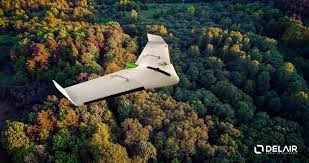
\includegraphics[width=\textwidth]{Imagenes/dron.jpg}
     \hfill
     \caption{Acá puede ir o no una imagen ilustrativa; revisar que esté referenciada correctamente}
    \label{dron}
\end{figure}

\subsection{Plataformas para el sensado remoto}
En este apartado se analizarán las principales características de las opciones de plataformas para el sensado remoto. El análisis se limitará a la opción de uso de sensores de espectro visible.
Los sensores remotos que serán tratados en el presente trabajo son del tipo pasivo, es decir, están compuestos por detectores que registran las ondas de luz solar reflejadas en el terreno. Particularmente nos interesan los que cubren el espectro visible. Básicamente constituyen una cámara fotográfica, que se compone de un arreglo de lentes y espejos que refractan y reflejan la luz, proyectándola sobre un sensor fotosensible, generalmente es un rectángulo conformado como un arreglo de detectores, cada uno de ellos representa a un pixel de la imagen. Según las características de estos sensores y la configuración de lentes, la distancia al objetivo, la resolución espacial queda determinada. 
\subsubsection{Imaginería satelital}
Se entiende por satélite artificial a todo dispositivo fabricado por el humano que es puesto en órbita alrededor del planeta Tierra con diversos propósitos que abarcan desde el establecimiento de comunicaciones hasta la observación terrestre por medio del sensado remoto. Éste último es el que reviste interés para el presente trabajo. Los satélites para sensado remoto van generalmente equipados con sensores multiespectrales, con múltiples bandas. La operación de los satélites es de manera continua desde que son puestos en órbita hasta el fin de su vida útil, varios años después. El lanzamiento y puesta en órbita requiere de infraestructura adecuada a tal fin, de las cuales hay muy pocas en el mundo, concentradas en no más de una decena de países. Los datos recopilados por los satélites son transmitidos a estaciones terrenas ubicadas en distintos puntos del planeta, y el acceso a las imágenes de alta resolución suele ser restringido a una contraprestación monetaria. No obstante suele haber acceso gratuito a imágenes con menor resolución. Las imágenes satelitales se definen por sus características de resolución, que son cuatro: resolución espacial, espectral, temporal y radiométrica.

Según la base de datos de la Unión de Científicos Conscientes \cite{noauthor_satellite_nodate}, actualizada el primero de mayo de 2.022, existen alrededor de 5.500 satélites orbitando la Tierra, de los cuales 1.156 (es decir un 21\%)tienen por finalidad la observación terrestre. Son utilizados varios tipos de sensores considerando el rango de frecuencias o la longitud de onda para cuya adquisición han sido diseñados. Se destacan los de luz visible, infrarrojo cercano (near infrared - NIR), infrarrojo térmico (thermal infrared - TIR), pancromático e infrarrojo de onda corta (shortwave infrared - SWIR). También existe un considerable despliegue de radares de apertura sintética (synthetic aperture radar - SAR) en diferentes bandas. De los satélites de observación terrestre, aproximadamente un 40\% son con sensores ópticos, es decir, capturan imágenes en el espectro visible.
Hay muchas y muy diversas fuentes de imágenes satelitales, tanto en forma gratuita como pagas. Entre las opciones pagas, imágenes multiespectracles con una resolución espacial de 50 cm se consiguen por montos entre 10 dólares por km\textsuperscript{2} hasta 29 dólares por km\textsuperscript{2} según sean actualizadas o de archivo (más de 90 días)\cite{noauthor_satellite_2020}. Debe tenerse en cuenta el tamaño mínimo del área a ser adquirida, en caso de las imágenes de archivo son 25 km\textsuperscript{2} (2500 ha) y las actualizadas son de 100 km\textsuperscript{2} (10000 ha).
\begin{table}[H]
    \centering
    \caption{Características de sensores satelitales. Fuente \cite{noauthor_3_nodate}}
    \begin{tabular}{c p{20mm} p{15mm} p{15mm} p{25mm} p{20mm}p{20mm} p{20mm}|}
        \hline
        \hline
        \textbf{Sensor} & \textbf{Tamaño de imagen} & \multicolumn{4}{c}{\textbf{Resolución}} & \textbf{Aplicación principal} \\
        %\hline
        & & \textbf{Espacial} & \textbf{Temporal} & \textbf{Radiométrica} & \textbf{Espectral}  &\\
        \hline \hline
        Meteosat & Toda la esfera & 	2500 m 	& 0.5 h 	& 256 ND 	& 1Vis 1IR 1 IT & Meteorología\\
        \hline
        NOAA AVHRR & 2700 x 2700 km	& 1100 m 	 	& 12 h 	& 1024 ND 	& 2Vis 1IR 1IT & Observación atmosférica\\
        \hline
        Landsat TM 	& 185 x 185 km & 30 m 	 	& 16 d 	& 256 ND 	& 3Vis 3IR 1IT & Observación terrestre\\
        \hline
        SPOT HRV & 60 x 60 km	& 20 m 	 	& 20 d	& 256 ND 	& 2Vis 1IR & Observación terrestre\\
        \hline
        SPOT Vegetation & 2200 x 200 km	& 1150 m 	 	& 1 d	& 1024 ND 	& 2Vis 2IR & Monitoreo agrícola\\
        \hline
        MODIS & 2330 x 2330 km	& 250 - 100 m 	 km 	& 1 d	& 1024 ND 	& 36 bandas & Observación terrestre\\
        \hline
        IKONOS & 100 x 100 km	& 4 m 	 	& 3 d 	& 2048 ND 	& 3Vis 1IR & Observación terrestre\\
        \hline
        Albedo & 35 x 7 km & 0,4 m  & 1 d & S/D & 3Vis 1IR & Observación terrestre\\
        \hline
         Worldview & 13 x 13 km &   & 1 d & 2048 & 29 bandas & Observación terrestre\\
        \hline
         Sentinel & 13 x 13 km &  10 m & 1 d & S/D & 13 bandas & Observación terrestre\\
        \hline
        \hline
    \end{tabular}

\label{Satelites}
\end{table}
\subsubsection{Aeronaves convencionales tripuladas}
Aquí se agrupan las aeronaves de determinado porte, cuya operación debe hacerse con tripulación, requiriendo que sea personal capacitado y con licencia para operarlos. En esta categoría se incluyen los aviones de ala fija, como los de ala rotatoria (helicópteros) así como aerostatos. Su operación requiere de una planificación de vuelo que debe ser reportada al área de espacio de vuelo controlado, además de necesitar una base de despegue y aterrizaje. El marco regulatorio de estas operaciones son las Regulaciones Argentinas de la Aviación Civil (RAAC), Parte 91 \cite{noauthor_infoleg_nodate-1}.
\paragraph{Cámaras fotográficas}
Algunos tipos de cámaras utilizadas a bordo de aeronaves tripuladas para realizar relevamientos fotogramétricos:
Vexcel UltraCam Eagle

%Se podría añadir como figura un mapa con las regiones de información de vuelo (FIR), con las zonas de control, aeródromos habilitados, por ejemplo, etc.
\subsubsection{Aeronaves no tripuladas}
Generalmente conocidos como VANT, los vehículos aéreos no tripulados (VANT) son cada vez más asequibles por el público general. Disponibles en amplia variedad de modelos, constituyen una formidable herramienta para llevar a cabo tareas de relevamiento aéreo. El abanico de posibilidades se ve ampliado por la prescindencia de una pista de despegue o aterrizaje de dimensiones grandes. El marco legal regulatorio para la actividad con VANT es la resolución ANAC 885 \cite{noauthor_infoleg_nodate}.
Existe una amplia variedad de tipos de VANT, que pueden ser de múltiples rotores o de ala fija. El propósito del presente trabajo no es exhaustivo en este aspecto, pero a los efectos de describir las características principales, se lo hará con algunos de ellos.
\paragraph{Multirrotor}
Los VANT tipo multirrotor poseen cuatro o más hélices para proporcionar al vehículo la sustentación y la propulsión en tres ejes de desplazamiento. Esta característica es la que le confiere mayor maniobrabilidad, especialmente en espacios reducidos. La energía para propulsarse es eléctrica, proveniente de baterías. Son los más difundidos comercialmente.
\subparagraph{DJI Mini 2}
Un dron comercial asequible es el Mini 2 del fabricante DJI \cite{noauthor_dji_nodate-1}. Está equipado con una cámara con sensor 1/2.3” CMOS, de 12 millones de píxeles efectivos. La lente de la cámara posee un ángulo de visión de 83º y un formato equivalente a 35 mm de longitud focal de 24 mm, una apertura de f/2.8 y un rango focal de 1 m hasta infinito. En cuanto a las velocidades, el dron tiene tres modos de funcionamiento, modo Sport, modo Normal y modo Cine. En Sport se desplaza hasta 16 m/s, en modo normal 10 m/s y en modo cine 6 m/s.
\subparagraph{DJI Mavic 3M}
Este es un dron profesional \cite{noauthor_dji_nodate}. Cuenta con una cámara RGB de 4/3 CMOS, con 20 millones de píxeles efectivos. La lente es de un campo de visión de 84º, con una longitud focal equivalente de 24 mm. La apertura es de f/2.8 a f/11, y foco de 1 m al infinito. En modo normal puede desplazarse hasta 15 m/s
\paragraph{Ala fija}
Este tipo de VANT poseen un ala fija que le brinda sustentación, por lo que pueden incluso planear aunque falle la planta motriz de la aeronave. Sus características de funcionamiento permiten vuelos más extensos, cubriendo mayores áreas. Existen VANT de ala fija alimentados eléctricamente con baterías o con motores de combustión interna. Se los encuentra esencialmente en aplicaciones de agricultura de precisión y en el campo militar. 
\subparagraph{Asesor/9}
Es un VANT de ala fija de casi 2 m de envergadura \cite{noauthor_drone_nodate}. Puede desplazarse a 17 m/s y tiene una autonomía de dos horas de vuelo. Va equipado con una cámara multiespectral MicaSense Altum-PT \cite{noauthor_altum-pt_2023} cuyo sensor es de 12,4 millones de píxeles, que le confieren una resolución de 5,28 cm/pixel volando a 120 m sobre el terreno.

Sensor
12.4 MP sensor pancromático
Cinco bandas espectrales de 3.2 MP
Resolución
Multiespectral (pan-sharpened): 1.24cm/pixel a 60m; 2.49cm/pixel a 120m

RGB12.4 MP (obturador global, alineado con todas las bandas)
Sensor térmicoFLIR LWIR infrarrojo térmico 7.5-13.5um calibrado radiométricamente
RESOLUCIÓN5.28 cm cm / pixel (por banda MS), 33.5 cm / pixel (banda térmica), 2.49 cm / pixel (pancro) a 120 m AGL
VELOCIDAD DE CAPTURAHasta 3 capturas por segundo DNG sin procesar
INTERFACES3 GPIO: señal de disparo, salida de la parte superior del cuadro, salida de 1 PPS, botón host. Puerto USB 2.0 para WiFi, ethernet 10/100/1000, serial, y almacenamiento CFexpress
CAMPO DE VISIÓN50° HFOV x 38° VFOV (MS) / 44° HFOV x 38° VFOV (PAN)
\color{black}
\section{Procesamiento de imágenes (Bloque 2)}

\subsection{Concepto de imagen, espacios de color, entidad matricial)}
Conceptualmente la imagen es una representación de un objeto que puede o no existir realmente. Las características que distinguen y hacen a la particularidad de cada imagen es la forma en que sus elementos que la componen están ordenados y poseen sus características. En las imágenes digitales esos elementos que componen a una imagen se denominan píxeles, y desde el punto de vista algebraico, una imagen es representada como una matriz de ancho N y alto M determinados. A su vez cada píxel está caracterizado por composición de bandas o canales. Si la imagen es de color, en espectro visible, existen tres canales o bandas correspondientes al rojo (correspondiente al rango de 645-700 nm), verde (correspondiente al rango de 500-550 nm) y azul (470 nm). La combinación de las características de cada canal o banda constituirá el color con el que se percibe el píxel. De modo que si, con un ancho de palabra de ocho bits, cada banda se resuelve en $2^8=256$ (0-255) distintos niveles, cada píxel puede adoptar hasta más de 16 millones de colores.
En esta tesis nos enfocaremos en la imagen como representación de una porción de la superficie terrestre.\\
El proceso de obtención de imágenes tiene como punto de partida la captura, que consiste esencialmente en un recorte dimensional e instantáneo que es fijado en una plataforma, antiguamente una solución química, actualmente en forma electrónica, lo que permite su almacenamiento y procesamiento de manera digital. La imagen se genera por la interacción de energía en forma de onda electromagnética con la materia. La fuente de radiación electromagnética puede provenir del mismo objeto estudiado o puede ser de origen externo. De cualquier forma, la imagen del objeto estudiado se constituye a partir de la radiación electromagnética recibida, la cual puede ser por la propia radiación del objeto o por el reflejo de otra fuente de radiación. Los sensores fotográficos pueden ser pasivos o activos, según la capacidad de emitir radiación que es reflejada por el objeto y detectada por el sensor (activos, como es el caso de sensores SAR. LIDAR, etc.). Los sensores de las cámaras fotográficas están dispuestos en un arreglo matricial, de ese modo las imágenes pueden ser representadas por la entidad matemática matriz, constituida por píxeles. Las imágenes pueden ser monocromáticas o multiespectrales. En el primer caso la matriz es bidimensional, con ancho N y alto M. En el caso multiespectral será un arreglo multidimensional, el caso más general es el que se compone de tres bandas de color en el espectro visible, rojo, verde y azul, también conocido con el acrónimo RGB del idioma inglés. Bajo esa forma de representación, las imágenes pueden ser procesadas y sometidas a análisis mediante algoritmos computacionales. En general, previo al análisis de imágenes se suele aplicar un preprocesamiento que involucra algún tipo de filtrado, o algún ajuste de parámetros de la imagen, como el contraste o ecualizado de bandas. También suele realizarse alguna conversión entre diferentes espacios de color, según los requerimientos.\\
La imagen en tanto entidad algebraica computacional, es decir matriz, porta consigo información que puede ser procesada y analizada. Los métodos de análisis y procesamiento son muy variados y dependen del tipo de imagen y de información que se busca extraer. Con frecuencia son de utilidad los histogramas de las imágenes, los cuales consisten en ordenar los niveles de intensidad por canal o banda y graficar la cantidad de píxeles por cada nivel. También desde el aspecto morfológico es posible efectuar el análisis de imágenes estudiando cada pixel y sus alrededores, escudriñando la estructura de la imagen. De ese tipo de análisis surge la identificación de formas, de texturas.\\
Con otro tipo de enfoques es posible analizar las imágenes en elementos más sutiles o complejos, como puede ser la presencia de sombras. Previamente se puede suponer que los píxeles que corresponden a sombras son más oscuros que los otros, es decir, el valor de la intensidad del pixel es menor, pero en la realidad esto no es así, por lo que es necesario usar otras metodologías, como por ejemplo el método de invariante de color.
\subsection{Sombras en dosel selvático}
La presencia de sombras en las imágenes aéreas del dosel selvático puede ser de ayuda en el análisis de la estructura del dosel selvático, al aportar información sobre la eventual existencia de ejemplares de capa emergente. Asimismo puede ser un signo descriptivo de la estructura de la porción de selva estudiada, evidenciando claros, huecos en la selva que denoten algún tipo de acción extractiva, o la presencia de especies de flora exótica amenazantes.
\subsection{Filtrado homomórfico }
\subsubsection{C1-Lógica difusa y procesamiento homomórfico (sombras)}
Según el modelo Stockham \cite{stockham_image_1972} una imagen puede descomponerse en dos partes, una la denominada iluminación y la otra componente es la reflexión. Llevadas al plano de frecuencias, se confirma el hecho de que la componente de iluminación tiene una variación más lenta, es decir, se corresponde con las frecuencias bajas. De modo similar, la componente de reflexión se corresponde con frecuencias altas \cite{oppenheim_nonlinear_1968}. Entendiendo esto, es factible implementar un filtrado en la imagen para realzar las sombras, separando la componente de iluminación de la de reflexión. Esta técnica fue utilizada en la remoción de sombras en imágenes de piezas de manufactura \cite{yang_research_2012} y en la detección automática de sombras en objetos oscuros \cite{etemadnia_automatic_2003}. En el presente trabajo, la aplicación a la detección de especies arbóreas es novedosa. 
\subsection{Procesamiento morfológico (Wagner)}
Una réplica del trabajo de \cite{ferreira_tree_2019}
Partiendo de una imagen en escala de grises, se realizó una secuencia de pasos en los que se implementan diferentes filtros para identificar cada una de las copas, de un modo que finalmente se obtuvo una imagen binarizada con la cual se pudo obtener un conteo de las copas. El primer paso consistió en hacer una clara identificación de los bordes y del área de copas. Luego se aplicó un algoritmo de Rolling Ball \cite{sternberg_biomedical_1983} que produce un suavizado en los niveles de grises dentro de las copas. En una siguiente etapa, distinguiendo copas grandes de pequeñas, se identificaban huecos en las copas grandes, para posteriormente rellenarlos con un valor promedio. Una vez rellenos todos los huecos y uniformadas todas las copas, se procede a segmentarlas, obteniéndose una imagen binarizada, con cada copa de árbol aislada e identificada en su posición.
El tratamiento automático de clasificación de especies arbóreas a partir de imágenes requiere de un conjunto de habilidades informáticas que van desde la manipulación el tratamiento de
las imágenes hasta el entrenamiento de modelos de aprendizaje automático. Para obtener una
aceptable clasificación de copas es necesario realizar procesamiento a la imagen
aprovechando las características de textura y contraste que ésta exhibe. Los algoritmos
matemáticos desarrollados en este trabajo posibilitan una adecuada segmentación de las
copas individuales del dosel y capa emergente de la Selva Atlántica, lo que consecuentemente
habilita en otro nivel la clasificación por especies. Para obtener el segmentado se toma como
punto de partida la imagen aérea en escala de grises, ya que se enfoca en los diferentes
contrastes y texturas existentes entre el área de copas y el espacio entre ellas. Corresponde
hacer una primer etapa de identificación gruesa entre copas y bordes, luego se homogeneiza el
interior de las copas para eliminar huecos. La imagen es tratada matemáticamente como una
matriz donde cada elemento es un píxel, cuyo valor se relaciona con la intensidad
correspondiente al espacio de color HSI. Esta matriz es pasible de manipulación matemática,
de modo que permite aplicársele filtros varios, algoritmos de procesamiento morfológicos, que
permiten resaltar estructuras internas de la imagen, facilitando esto la segmentación de copas.
Se aplica un criterio de distinción de tamaño de copas grandes y chicas, partiendo desde la
resolución espacial de la imagen, definiendo aquellas grandes como las que superan el radio
de tres píxeles. Diferentes algoritmos se aplican de forma secuenciada, procesando sobre los
resultados de cada paso anterior. De modo que intervienen algoritmos de homogeneización
como el filtro RollingBall, el filtrado top-bottom-hat basado en operadores morfológicos de apertura y clausura. En cada etapa se definen parámetros que se ajustan según las condiciones
de la imagen, algunos de los cuales se obtienen por medio de herramientas de estadística
(promedio, percentiles, etc.). Estos son tenidos en cuenta para definir umbrales de decisión. A
los fines de visualizar el comportamiento de los algoritmos y la influencia de estos parámetros,
se condujo una evaluación tipo “gridsearch” en la que se definió un rango para cada parámetro
y se expuso el resultado correspondiente. Esta pasantía se desarrolla en linea con los objetivos
propuestos en el plan de trabajo de la tesis doctoral relacionada con la detección automática
de especies de árboles nativos en la selva atlántica. 
%\color{cyan} %color de texto con 70-80 % o más de avance
\subsection{Invariante de color (paper turco)}
%\color{cyan}
\subsection{C2-Índice invariante de color (sombras)}
Un método que dio resultados interesantes en la detección de sombras es el que implementaba el cálculo del índice invariante de color (IIC). Probando con distintos valores de umbral, se observó que el que producía resultados más satisfactorios era el que correspondía al 85º percentil de la distribución de los valores de IIC.
El punto de partida del método es la adquisición de imágenes aéreas. No hay requerimientos especiales, excepto que se den las condiciones para proyección de sombras. Se tomaron imágenes de un área representativa de la selva nativa en la provincia de Misiones, las cuales fueron capturadas desde un VANT que sobrevoló las áreas de interés. A los efectos de obtener imágenes con presencia de sombras, se estableció un adecuado rango temporal de captura de imágenes, en este caso de 3 a 4 pm. Las imágenes fueron adquiridas en el invierno meridional, en el mes de agosto, cuando la proyección de sombras es mayor debido a la posición relativa del sol. Se utilizó un dron Mini 2, del fabricante DJI, equipado con una cámara de 12 megapíxeles. La altura de vuelo sobre el terreno fue de 50 metros. la resolución espacial de las imágenes son de 3 cm/píxel.
\subsubsection{Introducción IIC}
La conservación de áreas naturales forestales tiene cada vez mayor relevancia a nivel mundial debido a que los bosques nativos tienen un rol probado en la mitigación del cambio climático. En ese sentido se han propuestos numerosas acciones usando diversas herramientas para ayudar a conservar los bosques. Entre dichas herramientas el relevamiento y monitoreo de bosques mediante imágenes aéreas es un campo promisorio. En particular el monitoreo de la Selva Atlántica es un tópico que ha recibido mucha atención en las últimas décadas, desgraciadamente porque se ha convertido en uno de los ecosistemas más amenazados en el mundo. Siendo originalmente de una extensión de 1.290.692,46 km$^2$ durante los últimos siglos, que abarcaba parte de Brasil, Argentina y Paraguay, hoy la Selva Atlántica está reducida a casi 162.000 km$^2$, lo que representa sólo un 12,4 \% de la extensión original \cite{de_lima_erosion_2020}, y se ubica principalmente en la Provincia de Misiones en Argentina. A pesar de de este escenario adverso, la diversidad de especies que habitan en la Selva Atlántica es aún una de las más grandes del mundo \cite{lima_how_2015}. Sin embargo algunas especies de fauna y flora están en un estado de conservación crítico, como por ejemplo algunas especies de árboles cuya copa sobresale del dosel, situándose en lo que se conoce como capa emergente, a treinta metros o más respecto del suelo \cite{noauthor_rainforest_2015}, por lo que sería recomendable conocer la cantidad y geolocalización de este tipo de árboles. También sería de interés determinar la distribución y localización de algunas especies como bambú y lianas, que podrían ser indicadores de niveles de preservación \cite{bedrij_selective_2022}. En este contexto el monitoreo forestal representa un rol crítico en la evaluación de la eficacia de estrategias de restauración, identificando acciones correctivas, comparando resultados entre proyectos y aprendiendo de proyectos pasados para determinar futuros lineamientos en restauración \cite{viani_protocol_2017}
El nivel de preservación de la Selva Atlántica ha sido evaluado con varios métodos. El más difundido es la exploración in situ, restringido a áreas pequeñas, con posibilidad de ser extrapolados los resultados a áreas más grandes con el correspondiente error de estimación. En esta forma tradicional, el monitoreo forestal es una tarea ardua y demandante de tiempo, por lo que al transcurrir el tiempo entre revisitas, las condiciones ambientales podrían haber cambiado de modo considerable. Además el desplazamiento dentro de la selva resulta difícil y puede generar disturbios en la flora y en la fauna locales. Todo esto puede evitarse con el monitoreo forestal por medio de análisis de imágenes aéreas o satelitales. Éstas últimas representan una fuente interesante de datos, principalmente debido al inmenso área que puede cubrir una simple escena (cientos de kilómetros cuadrados) con múltiples bandas espectrales, especialmente más allá del espectro visible. Sin embargo tienen usualmente una relativamente baja resolución espacial y baja disponibilidad. En el mejor de los casos la resolución espacial de estas imágenes está en el orden de 30 cm por pixel \cite{poli_radiometric_2014}, siendo su adquisición onerosa, que puede ser de varios miles de dólares por cada escena \cite{noauthor_geocento_2022}. La obtención de estas imágenes está condicionada a la disponibilidad en el tiempo, ya que en algunos casos la frecuencia de revisita de determinados sitios puede ser de varios días \cite{li_global_2017}.
A pesar de estas desventajas, varios trabajos han relevado especies arbóreas y recolectado datos forestales usando imágenes satelitales con alta resolución espacial y espectral \cite{gomes_detection_nodate,cross_classification_2019,abd_latif_determination_2012,ferreira_tree_2019,radoux_quantitative_2007}. Por otro lado, otros trabajos han monitoreado bosques usando otras herramientas como los vehículos aéreos no tripulados (VANT) \cite{albuquerque_remotely_2020,albuquerque_forest_2021,qin_individual_2022,machida_modeling_2022}, en la detección de flores \cite{campbell_simple_2018} o incorporando sensores LiDAR \cite{terryn_quantifying_2022,brede_non-destructive_2022}. La combinación de imágenes aéreas o satelitales de alta resolución espacial con herramientas computacionales facilita la implementación del mapeo del estado de salud forestal \cite{prost_discrimination_2008} o el conteo automático de árboles \cite{putra_automatic_2023}. Las imágenes aéreas obtenidas con VANT poseen algunas ventajas sobre las satelitales, entre las que se encuentra su relativo bajo costo, su muy alta resolución espacial y su baja altitud de sobrevuelo, lo cual permite evitar interferencias de nubes \cite{alexander_locating_2018,ahmad_aerial_2010,zhang_seeing_2016,ahmad_digital_2013,colomina_unmanned_2014,eisenbeiss_mini_nodate}. No obstante, la combinación de la posibilidad de captura de imágenes de grandes extensiones de selva con una adecuada resolución espacial para luego procesar esas imágenes con métodos y tecnologías que ofrecen resultados aceptables sin excesivas demandas computacionales y requerimientos tecnológicos no es tan sencilla de implementar. La clave para alcanzar esa meta es trabajar con un atributo de la imagen que puede ser extraído con algoritmos eficientes. En este estudio asumimos que puede explorarse la información contenida en regiones sombreadas de imágenes aéreas de regiones forestales mediante algoritmos computacionales de bajo costo.
Las sombras se producen por oclusión por parte de un objeto de forma total o parcial de la luz directa emanada de la fuente \cite{hu_revisiting_2021}. En la bibliografía se considera que las sombras en imágenes de sensado remoto pueden ser originados por tres causas: material natural o urbano (árboles o edificios), características topográficas (colinas o montañas) y nubes \cite{shahtahmassebi_review_2013}. La presencia de sombras en imágenes de sensado remoto es objeto de muchas consideraciones. En algunos casos las sombras pueden ser una fuente de información útil, proveyendo por ejemplo una perspectiva en tres dimensiones de una escena capturada, mientras que en otros casos la presencia de sombras dificulta la recolección de datos detallados. Hay por lo tanto numerosos trabajos sobre el procesamiento de imágenes con sombras \cite{shahtahmassebi_review_2013,mostafa_review_2017,freitas_automatic_2017,chang_c_evaluation_2016}. Algunos trabajos están basados en el modelo de Stockham \cite{stockham_image_1972}, implementando el filtrado homomórfico para la remoción de sombras \cite{yang_shadow_2007} o para la detección de sombras en imágenes aéreas de selvas \cite{bernhardt_deteccion_2017}. Para la detección de sombras puede utilizarse como base la invariancia de color \cite{gevers_content-based_1999,geusebroek_color_2001}. En el presente trabajo nos enfocamos en el procedimiento de detección de sombras partiendo de tres hipótesis, la primera de las cuales es que las sombras que son causadas por depresiones en el dosel selvático y por la presencia de especímenes de capa emergente pueden ser detectadas de manera automática en las imágenes aéreas. La segunda hipótesis es que se puede utilizar índices invariantes de color para obtener una clasificación de píxeles de la imagen según corresponda a una región sombreada o no. Y la tercera hipótesis es que ciertas características presentes en el histograma de la imagen permiten automatizar la determinación de el umbral para binarizar la imagen en sendas regiones, sombreadas y no sombreadas.
En resumen, la propuesta del presente estudio es un método de detección automática de sombras en imágenes aéreas de selvas, basado en el cálculo del índice invariante de color \cite{sirmacek_damaged_2009} que se obtiene al combinar dos de los tres canales RGB de la imagen. Además la metodología propuesta demuestra la utilidad del percentil en la frecuencia de distribución del índice invariante de color para la obtención del umbral de binarización, lo cual permite la automatización de la segmentación de sombras en la imagen de un modo relativamente simple. El objetivo principal de este trabajo es obtener un método fiable para detección de sombras usando las fácilmente obtenidas y ampliamente difundidas imágenes RGB, con base en métodos computacionales poco demandante en cuanto a recursos.
Los detalles de la metodología propuesta se desarrollan en la sección \ref{Metodología}. La validación es descripta en \ref{Validacion}, y los resultados se muestran en \ref{Resultados}. Finalmente las conclusiones son discutidas en \ref{Conclusiones}

\color{black}


\chapter{Metodología}
    \section{Sensado remoto, plataformas (¿?) (Bloque 1)}

\section{Procesamiento de imágenes (Bloque 2)}

\subsection{Filtrado homomórfico (CRICTE 2017)}
\subsection{Procesamiento morfológico (Pasantía)}
\subsection{Invariante de color (paper RSASE)}
\subsection{Machine learning (¿?)}




Las Tesis  en el marco de la Carrera del Doctorado en Ciencias Aplicadas (DCA) deberán ser escritas en idioma Español, utilizando letra tipo Arial, tamaño 11 puntos, y formato de hojas tipo A4, numeradas en el margen inferior derecho, con interlineado 1,5; sin separación automática de sílabas al fin de línea y con los cuatro márgenes de 2,5 cm.

El contenido de las Tesis deberá incluir los siguientes ítems y en el siguiente orden:\newline
●	Carátula (con el formato solicitado por el DCA que se adjunta al presente Anexo)\newline
●	Agradecimientos\newline
●	Índice\newline
●	Listado de Abreviaturas (en caso de que lo considere conveniente)\newline
●	Resumen en Español\newline
●	Palabras Claves en Español (tres a seis palabras claves separadas por comas. La primera letra de cada palabra clave debe empezar con mayúscula)\newline
●	Resumen en Inglés (Abstract)\newline
●	Palabras Claves en Inglés (tres a seis palabras claves separadas por comas. La primera letra de cada palabra clave debe empezar con mayúscula)\newline
●	Capítulo 1: Introducción (deberá contener el planteo del problema a resolver, los objetivos generales y específicos y una breve explicación de lo que versará la Tesis)\newline
●	Capítulo 2: Marco Teórico\newline
●	Capítulo 3: Metodología\newline
●	Capítulo 4: Resultados y Discusión (O bien, se podrá presentar en dos Capítulos separados: Capítulo 4: Resultados y Capítulo 5: Discusión)\newline
●	Capítulo 5: Conclusiones (Deben presentarse en párrafos cortos y concretos. No deben hacer referencia a trabajos futuros ni a hipótesis no incluidas en el trabajo).\newline
●	Recomendaciones para Trabajos Futuros\newline
●	Producción Científica (surgida del trabajo de Tesis)\newline
✔	Publicaciones en Revistas y Capítulos de Libros\newline
✔	Presentaciones a Congresos\newline
●	Proyecto/s de Investigación dentro del/los cual/es se desarrolló la Tesis (si hubiera/n)\newline
●	Beca/s y Subsidio/s con los que se financió la Tesis (si hubieran)\newline
●	Apéndices o Anexos (se reservan para detallar técnicas originales utilizadas o análisis teóricos que impedirían seguir fluidamente el trabajo si se incluyeran en el texto). Las tablas y figuras de los apéndices o anexos deben comenzar otra numeración diferente a la de los capítulos.\newline

Aclaraciones

⮚	El listado de Referencias bibliográficas se podrá incorporar al final de cada capítulo, ó todas juntas al final de la Tesis, las mismas serán listadas en el orden en que aparecen citadas en el texto. \newline
Formato de las Referencias\newline
Estilo de las Referencias\newline
En el texto de la Tesis: indique las referencias por número (s) entre corchetes en línea con el texto. Cuando se menciona a los autores, siempre se deben proporcionar los números de referencia.
Ejemplo: '..... como se demostró [3,6]. Barnaby y Jones [8] obtuvieron un resultado diferente ... '
Lista de Referencias\newline
Numere las referencias (números entre corchetes) en la lista en el orden en que aparecen en el texto, como se indica a continuación:
\paragraph{Referencia a una publicación de revista}
[1] J. van der Geer, J.A.J. Hanraads, R.A. Lupton, The art of writing a scientific article, J. Sci. Commun. 163 (2010) 51–59.https://doi.org/10.1016/j.Sc.2010.00372.
\paragraph{Referencia a una publicación de revista con un número de artículo}
[2] J. van der Geer, J.A.J. Hanraads, R.A. Lupton, 2018. The art of writing a scientific article.Heliyon. 19, e00205.https://doi.org/10.1016/j.heliyon.2018.e00205.
\paragraph{Referencia a un libro}
[3] W. Strunk Jr., E.B. White, The Elements of Style, fourth ed., Longman, New York, 2000.
\paragraph{Referencia a un capítulo en un libro editado}
[4] G.R. Mettam, L.B. Adams, How to prepare an electronic version of your article, in: B.S. Jones, R.Z. Smith (Eds.), Introduction to the Electronic Age, E-Publishing Inc., New York, 2009, pp. 281–304.
\paragraph{Referencia a un sitio} web
[5] Cancer Research UK, Cancer statistics reports for the UK. http://www.cancerresearchuk.org/ aboutcancer/statistics/cancerstatsreport/, 2003 (accessed 13 March 2003).
\paragraph{Referencia a un conjunto de datos: [conjunto de datos]}
[6] M. Oguro, S. Imahiro, S. Saito, T. Nakashizuka, Mortality data for Japanese oak wilt disease and surrounding forest compositions, Mendeley Data, v1, 2015. https://doi.org/10.17632/ xwj98nb39r.1
⮚	Las figuras (gráficos, cuadros, fotografías, otros) deberán numerarse correlativamente en el orden de aparición en el texto y deberán incluir un breve título explicativo en la parte inferior de la figura. Las imágenes y fotografías se designarán como figuras.\newline
%%%%%%%%%%%%%%%%%%%%%%%%%%%%%%%%%%%%%%% FIGURA %%%%%%%%%%%%%%%%%%%%%%%%%%%%%%%%%%%%%%%%%%%%%%%%%%%%%%%%%
%\begin{figure}[ht!]
%    \centering
%    \captionsetup{justification=centering}
%    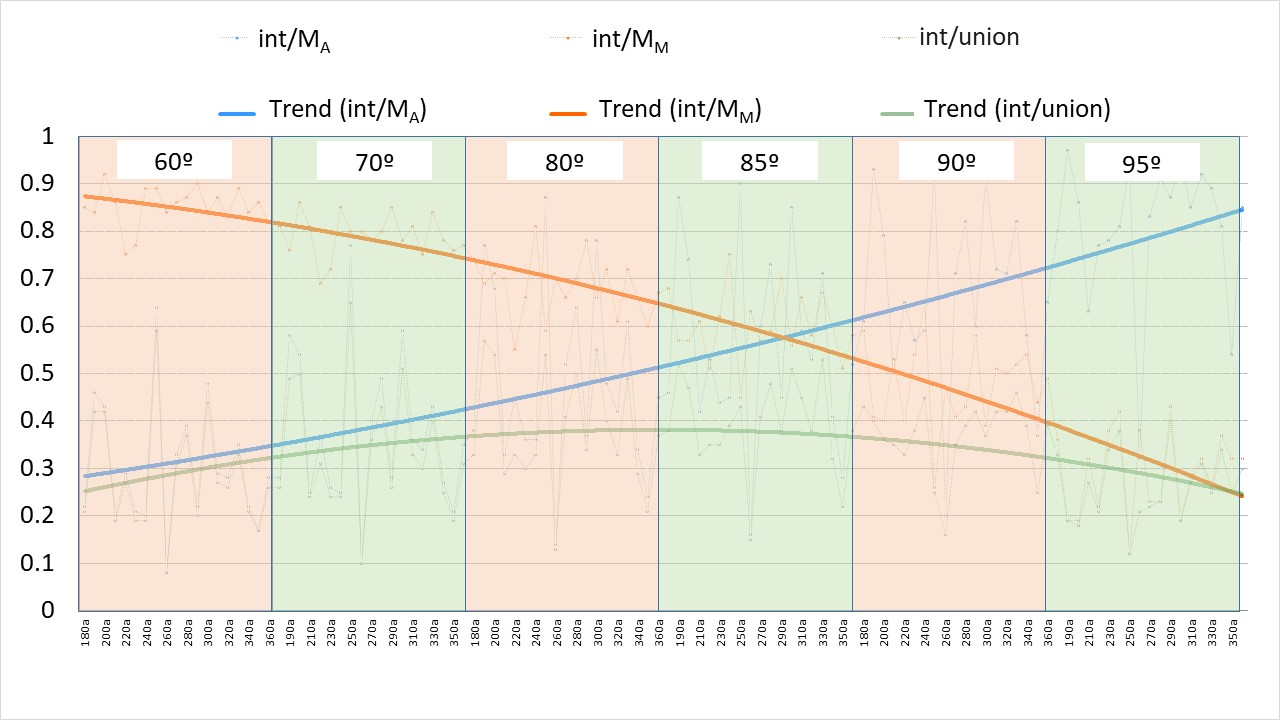
\includegraphics[width=8cm]{grafico.jpg}
%    \caption{Quality Index as a function of the percentile, for the different forest image used. QI\textsubscript{1} in orange, QI\textsubscript{2} in blue and QI\textsubscript{3} in green. The invariant color index used is ψ\textsubscript{BR}}	
 %   \label{qi}
%\end{figure}
%%%%%%%%%%%%%%%%%%%%%%%%%%%%%%%%%%%%%%%%%%%%%%%%%%%%%%%%%%%%%%%%%%%%%%%%%%%%%%%%%%%%%%%%%%%%%%%%%%%%%%%%%
⮚	Las tablas deberán numerarse correlativamente según su orden de aparición en el texto y en forma independiente de las figuras. Deberán incluir un título explicativo en su parte superior. De ser necesario se agregarán al pie notas explicativas para detallar abreviaturas, signos, medidas, otros, de tal manera que el lector pueda comprender su contenido sin recurrir al texto.
%%%%%%%%%%%%%%%%%%%%%%%%%%%%%%%%%%%%%%%%% TABLA %%%%%%%%%%%%%%%%%%%%%%%%%%%%%%%%%%%%%%%%%%%%%%%%%%%%%%%%%
\begin{table}[H]
    \centering
    \caption{Evaluation of the superposition of both masks. the manual and the automatic. carried on by the group of experts}
    \begin{tabular}{|c|c|c|c|c|c|c|c|}
       \hline
        COLOR INVARIANT INDEX & \multicolumn{6}{ |c|}{\textpsi \textsubscript{BR}}\\%\multicolumn{6}{ }{ |c|} \\
        \hline
        PERCENTILE & 60 & 70 & 80 & 85 & 90 & 95\\
        \hline
        GOOD & 0.0 & 0.0 & 4.5 & 15.8 & 20.5 & 0.0\\
        \hline
        REGULAR & 0.0 & 4.5 & 27.3 & 21.1 & 54.5 & 57.9\\
        \hline
        BAD & 100.0 & 95.5 & 68.2 & 63.2 & 25.0 & 42.1\\
        \hline
        COLOR INVARIANT INDEX & \multicolumn{6}{ |c|}{\textpsi \textsubscript{BG}}\\
        \hline
        PERCENTILE & 60 & 70 & 80 & 85 & 90 & 95\\
        \hline
        GOOD & 0.0 & 0.0 & 0.0 & 5.3 & 5.3 & 5.3\\
        \hline
        REGULAR & 0.0 & 5.3 & 10.5 & 15.8 & 42.1 & 21.1\\
        \hline
        BAD & 100.0 & 94.7 & 89.5 & 78.9 & 52.6 & 73.7\\
        \hline
        COLOR INVARIANT INDEX & \multicolumn{6}{|c|}{ \textpsi \textsubscript{GR}}\\
        \hline
        PERCENTILE & 60 & 70 & 80 & 85 & 90 & 95\\
        \hline
        GOOD & 0.0 & 0.0 & 0.0 & 0.0 & 0.0 & 0.0\\
        \hline
        REGULAR & 0.0 & 0.0 & 0.0 & 0.0 & 15.8 & 15.8\\
        \hline
        BAD & 100.0 & 100.0 & 100.0 & 100.0 & 84.2 & 84.2\\
        \hline
    \end{tabular}
    \\
    \raggedleft
    \label{tablita}
\end{table}
%%%%%%%%%%%%%%%%%%%%%%%%%%%%%%%%%%%%%%%%%%%%%%%%%%%%%%%%%%%%%%%%%%%%%%%%%%%%%%%%%%%%%%%%%%%%%%%%%%%%%%%%%
⮚	Las fórmulas y expresiones matemáticas deberán ser escritas dejando dos espacios sobre, debajo y entre cada una de ellas.
%%%%%%%%%%%%%%%%%%%%%%%%%%%%%%%%%%%%%% ECUACIÓN %%%%%%%%%%%%%%%%%%%%%%%%%%%%%%%%%%%%%%%%%%%%%%%%%%%%%%%%%
\begin{equation}
	\psi=\frac{4}{\pi} arctan\left(\frac{B\textsubscript{1}-B\textsubscript{2}}{B\textsubscript{1}+B\textsubscript{2}}\right),\label{eq1}
\end{equation}
%%%%%%%%%%%%%%%%%%%%%%%%%%%%%%%%%%%%%%%%%%%%%%%%%%%%%%%%%%%%%%%%%%%%%%%%%%%%%%%%%%%%%%%%%%%%%%%%%%%%%%%%%
Las fórmulas se ajustarán al margen izquierdo y serán numeradas correlativamente y entre paréntesis sobre el margen derecho. Debe quedar definido el significado y las unidades utilizadas en cada término de las expresiones.

⮚	Unidades: debe utilizarse el sistema internacional de unidades (SI).

\chapter{Resultados y Discusión}    
    %Se podrá presentar en dos Capítulos separados: Capítulo 4: Resultados y Capítulo 5: Discusión

%HIPÓTESIS: la linealidad se mantiene o no con la escala
\color{black} 
\section {Bloque/Núcleo 1-A1-Propuesta de relevamiento por imágenes RGB de las reservas de la provincia de Misiones}
%Comenzaría por una descripción territorial de las reservas, proponiendo una clasificación, que puede ser por público o privada, ubicación, superficie, etc. Luego vendría una propuesta de las opciones: satelital, aérea tripulada y aérea no tripulada, restringiendonos a imágenes RGB. Acompaña a cada opción un análisis técnico económico. Finalmente, concluir con cuál sería la mejor opción dependiendo del tipo de reserva y la resolución pretendida. Brindar una herramienta de toma de decisión para quien desee hacer un relevamiento de reservas en la provincia de Misiones.
%El propósito de esta sección es realizar un análisis comparativo del relevamiento entre distintas áreas de reservas forestales. Se consideran casos extremos en extensión grande como es la reserva Biósfera Yaboty, de más de 250 mil hectáreas, y por otro lado se analizan algunas reservas públicas o privadas de alrededor de pocas hectáreas de extensión. El objetivo es obtener herramientas que faciliten la toma de decisiones sobre la estrategia adecuada para el relevamiento y monitoreo forestal, tanto en el ámbito público como el privado, en la provincia de Misiones. Los parámetros que son considerados para el análisis son el tiempo que implica la captura de imágenes, la necesidad de recursos para almacenamiento, requerimientos económicos y restricciones legales y reglamentarias.
Con base en todos los cálculos, es posible establecer una comparación entre las distintas opciones de plataforma de sensado remoto, según el área relevada.
%% No olvidar mencionar que, por simplicidad en los cálculos se considera cada área como si fuera un cuadrado 
%%
En la tabla \ref{Tabla_borrador} se sumarizan los resultados, donde se puede observar de forma clara que para el caso de superficies relevadas de pocas hectáreas, el costo de obtención de las imágenes es significativamente inferior al de las imágenes satelitales. Esto se debe fundamentalmente a que la adquisición de imágenes satelitales requiere de una superficie mínima, 25 kilómetros cuadrados si las imágenes son de archivo (> 90 días)\cite{noauthor_satellite_2020}. Ya para el caso de superficies mayores como la reserva Yaboty, el costo total de captura de imágenes equipara e incluso supera al de imágenes satelitales. No solo termina siendo más oneroso el relevamiento fotográfico aéreo con VANT en grandes superficies, ya que adicionalmente se debe tener en cuenta la limitación de autonomía de esos vehículos, que generalmente no superan la media hora \cite{}, o la hora de autonomía en algunos casos \cite{}. Esto indudablemente afecta al flujo de trabajo por la necesaria reposición de baterías, a la vez que deben establecerse numerosas bases operativas en la medida en que se va avanzando con el relevamiento del terreno. Otra limitación que se suma a los VANT es el alcance que tiene el mando de control. Los VANT comerciales más difundidos suelen tener alcances de hasta 10 km \cite{} por lo que esto debe ser tenido en cuenta en la extensión del área a relevar. Por otro lado en el caso de las aeronaves tripuladas puede resultar muy inconvenientes en términos de erogación de dinero cuando se trata de pequeñas extensiones cuyo sobrevuelo de relevamiento no sobrepasa la hora de duración, ya que hay que sumar a toda la operatoria el traslado de la aeronave desde y hacia el aeródromo de base. Resulta evidente que será mayor la incidencia en el costo final la parte que corresponde al traslado en sí, si la superficie a ser relevada es de pocas hectáreas. En la provincia de Misiones existen en un radio menor a cincuenta kilómetros a las tres reservas analizadas algunos aeródromos o pistas que pueden usarse como base.
\begin{figure}
    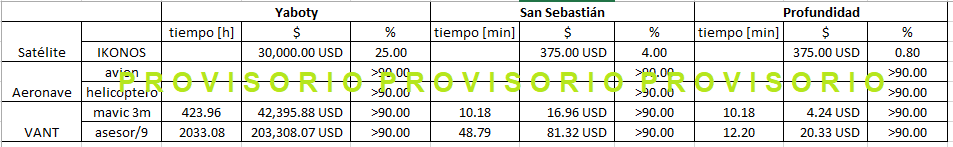
\includegraphics[width=\textwidth]{Imagenes/Tabla comparativa borrador.png}
     \hfill
     \caption{Tabla borrador}
        \label{Tabla_borrador}
\end{figure}
\subsubsection{Cálculo presupuestario}
Partiendo de las características del terreno a relevar (su extensión) y de la plataforma usada para la captura (dron con cámara/sensor) es posible acotar un marco presupuestario para llevar a cabo la tarea. Con los datos recabados puede afirmarse que para un relevamiento aéreo de un área pequeña de veinte hectáreas, es conveniente un VANT, ya que el costo total no excedería los 10 dólares, mientras que en un avión tripulado el costo total sería por lo menos diez veces, y una imagen satelital tendría un costo de 375 dólares. En el caso de un área un poco más grande, de cien hectáreas, el costo total con VANT sigue siendo más bajo que con las otras plataformas, con menos de 50 dólares. Finalmente para el caso de un área mucho más grande, de varios miles de hectáreas como la reserva Yaboty, se torna más conveniente el avión tripulado con alrededor de 20 mil dólares estadounidenses, un poco más que la mitad de lo que cuesta la imagen satelital, y muy por debajo del costo del VANT, que supera holgadamente el millón de dólares.
%%%%%%%%%%%%%%%%%%%%%%%%%%%%%%%%%%%%%%%%% TABLA %%%%%%%%%%%%%%%%%%%%%%%%%%%%%%%%%%%%%%%%%%%%%%%%%%%%%%%%%
% Please add the following required packages to your document preamble:
% \usepackage{multirow}
% \usepackage[table,xcdraw]{xcolor}
% If you use beamer only pass "xcolor=table" option, i.e. \documentclass[xcolor=table]{beamer}
% \usepackage[normalem]{ulem}
% \useunder{\uline}{\ul}{}
% Please add the following required packages to your document preamble:
% \usepackage{multirow}
% \usepackage[table,xcdraw]{xcolor}
% If you use beamer only pass "xcolor=table" option, i.e. \documentclass[xcolor=table]{beamer}
% \usepackage[normalem]{ulem}
% \useunder{\uline}{\ul}{}
% Please add the following required packages to your document preamble:
% \usepackage{multirow}
% \usepackage[table,xcdraw]{xcolor}
% If you use beamer only pass "xcolor=table" option, i.e. \documentclass[xcolor=table]{beamer}
% \usepackage[normalem]{ulem}
% \useunder{\uline}{\ul}{}
% Please add the following required packages to your document preamble:
% \usepackage{multirow}
% \usepackage[table,xcdraw]{xcolor}
% If you use beamer only pass "xcolor=table" option, i.e. \documentclass[xcolor=table]{beamer}
% \usepackage[normalem]{ulem}
% \useunder{\uline}{\ul}{}
% Please add the following required packages to your document preamble:
% \usepackage{booktabs}
% \usepackage{graphicx}
% Please add the following required packages to your document preamble:
% \usepackage{booktabs}
% \usepackage{graphicx}
% Please add the following required packages to your document preamble:
% \usepackage{booktabs}
% \usepackage{multirow}
% \usepackage{graphicx}
% Please add the following required packages to your document preamble:
% \usepackage{multirow}
% \usepackage{graphicx}
% Please add the following required packages to your document preamble:
% \usepackage{multirow}
% \usepackage{graphicx}
% \usepackage[table,xcdraw]{xcolor}
% If you use beamer only pass "xcolor=table" option, i.e. \documentclass[xcolor=table]{beamer}
\begin{landscape}
\begin{table}[]

    \caption{Comparación de los tiempos y costos para cada plataforma}
    \label{tab:tabla}
   
    \begin{tabular}{cc|ccc|ccc|ccc|c|}
    \cline{3-12}
    \multicolumn{2}{c|}{} &
      \multicolumn{3}{c|}{\cellcolor[HTML]{68CBD0}\textbf{Yaboty}} &
      \multicolumn{3}{c|}{\cellcolor[HTML]{68CBD0}\textbf{San   Sebastián}} &
      \multicolumn{3}{c|}{\cellcolor[HTML]{68CBD0}\textbf{Profundidad}} &
       \\ \cline{3-11}
    \multicolumn{2}{c|}{\multirow{-2}{*}{}} &
      \multicolumn{1}{c|}{\cellcolor[HTML]{68CBD0}\textit{Tiempo {[}h{]}}} &
      \multicolumn{1}{c|}{\cellcolor[HTML]{68CBD0}\textit{\$}} &
      \cellcolor[HTML]{68CBD0}\textit{\%} &
      \multicolumn{1}{c|}{\cellcolor[HTML]{68CBD0}\textit{Tiempo {[}min{]}}} &
      \multicolumn{1}{c|}{\cellcolor[HTML]{68CBD0}\textit{\$}} &
      \cellcolor[HTML]{68CBD0}\textit{\%} &
      \multicolumn{1}{c|}{\cellcolor[HTML]{68CBD0}\textit{Tiempo {[}min{]}}} &
      \multicolumn{1}{c|}{\cellcolor[HTML]{68CBD0}\textit{\$}} &
      \cellcolor[HTML]{68CBD0}\textit{\%} &
      \multirow{-2}{*}{\textbf{Resolución espacial {[}cm/pixel{]}}} \\ \hline
    \multicolumn{1}{|c|}{\cellcolor[HTML]{9698ED}} &
      \cellcolor[HTML]{9698ED}Pleiades &
      \multicolumn{1}{c|}{} &
      \multicolumn{1}{c|}{37,500.00 USD} &
       &
      \multicolumn{1}{c|}{} &
      \multicolumn{1}{c|}{375.00 USD} &
       &
      \multicolumn{1}{c|}{} &
      \multicolumn{1}{c|}{375.00 USD} &
       &
       \\ \cline{2-12} 
    \multicolumn{1}{|c|}{\cellcolor[HTML]{9698ED}} &
      \cellcolor[HTML]{9698ED}Satellogic &
      \multicolumn{1}{c|}{} &
      \multicolumn{1}{c|}{37,500.00 USD} &
       &
      \multicolumn{1}{c|}{} &
      \multicolumn{1}{c|}{375.00 USD} &
       &
      \multicolumn{1}{c|}{} &
      \multicolumn{1}{c|}{375.00 USD} &
       &
       \\ \cline{2-12} 
    \multicolumn{1}{|c|}{\multirow{-3}{*}{\cellcolor[HTML]{9698ED}\textbf{Satélite}}} &
      \cellcolor[HTML]{9698ED}IKONOS &
      \multicolumn{1}{c|}{} &
      \multicolumn{1}{c|}{37,500.00 USD} &
      ? &
      \multicolumn{1}{c|}{} &
      \multicolumn{1}{c|}{375.00 USD} &
      4.00 &
      \multicolumn{1}{c|}{} &
      \multicolumn{1}{c|}{375.00 USD} &
      0.80 &
      96.35 \\ \hline
    \multicolumn{1}{|c|}{\cellcolor[HTML]{9698ED}} &
      \cellcolor[HTML]{9698ED}Ala fija &
      \multicolumn{1}{c|}{69.13} &
      \multicolumn{1}{c|}{6,912.77 USD} &
      \textgreater{}90.00 &
      \multicolumn{1}{c|}{2.24} &
      \multicolumn{1}{c|}{3.74 USD} &
      \textgreater{}90.00 &
      \multicolumn{1}{c|}{0.42} &
      \multicolumn{1}{c|}{0.70 USD} &
      \textgreater{}90.00 &
      10.21 \\ \cline{2-12} 
    \multicolumn{1}{|c|}{\multirow{-2}{*}{\cellcolor[HTML]{9698ED}\textbf{Aeronave}}} &
      \cellcolor[HTML]{9698ED}Ala rotativa &
      \multicolumn{1}{c|}{} &
      \multicolumn{1}{c|}{} &
      \textgreater{}90.00 &
      \multicolumn{1}{c|}{} &
      \multicolumn{1}{c|}{} &
      \textgreater{}90.00 &
      \multicolumn{1}{c|}{} &
      \multicolumn{1}{c|}{} &
      \textgreater{}90.00 &
       \\ \hline
    \multicolumn{1}{|c|}{\cellcolor[HTML]{9698ED}} &
      \cellcolor[HTML]{9698ED}mavic 3m &
      \multicolumn{1}{c|}{8645.64} &
      \multicolumn{1}{c|}{ 1,685,899.92  USD} &
      \textgreater{}90.00 &
      \multicolumn{1}{c|}{5.12} &
      \multicolumn{1}{c|}{8.53 USD} &
      \textgreater{}90.00 &
      \multicolumn{1}{c|}{1.22} &
      \multicolumn{1}{c|}{2.04 USD} &
      \textgreater{}90.00 &
      10.23 \\ \cline{2-12} 
    \multicolumn{1}{|c|}{\cellcolor[HTML]{9698ED}} &
      \cellcolor[HTML]{9698ED}asesor/9 &
      \multicolumn{1}{c|}{21666.57} &
      \multicolumn{1}{c|}{ 4,224,981.67 USD } &
      \textgreater{}90.00 &
      \multicolumn{1}{c|}{10.38} &
      \multicolumn{1}{c|}{17.30 USD} &
      \textgreater{}90.00 &
      \multicolumn{1}{c|}{2.19} &
      \multicolumn{1}{c|}{3.66 USD} &
      \textgreater{}90.00 &
      5.34 \\ \cline{2-12} 
    \multicolumn{1}{|c|}{\multirow{-3}{*}{\cellcolor[HTML]{9698ED}\textbf{VANT}}} &
      \cellcolor[HTML]{9698ED}mini 2 &
      \multicolumn{1}{c|}{18854.06} &
      \multicolumn{1}{c|}{ 3,676,541.38 USD } &
      \textgreater{}90.01 &
      \multicolumn{1}{c|}{9.34} &
      \multicolumn{1}{c|}{15.57 USD} &
      \textgreater{}90.01 &
      \multicolumn{1}{c|}{2.25} &
      \multicolumn{1}{c|}{3.75 USD} &
      \textgreater{}90.01 &
      3.47 \\ \hline
    \end{tabular}%

\end{table}
\end{landscape}
%%%%%%%%%%%%%%%%%%%%%%%%%%%%%%%%%%%%%%%%%%%%%%%%%%%%%%%%%%%%%%%%%%%%%%%%%%%%%%%%%%%%%%%%%%%%%%%%%%%%%%%%%



\section{ Propuesta de Herramientas de Bajo Costo (Económico y Computacional) para el relevamiento del bosque atlántico}
%\subsection{RESULTADOS Relación de iluminación natural con histogramas de color}
%Con el objeto de evaluar la correspondiente afectación en el histograma de las imágenes capturadas respecto a las condiciones de iluminación natural, se hicieron varias capturas en distintos horarios durante varios días desde una posición fija a un determinado objeto (un árbol de palta) y se midió la iluminancia usando un luxómetro.
\color{cyan} %color de texto con 70-80 % o más de avance
\subsection{RESULTADOS Replicación del paper de Wagner}
Con base en el trabajo realizado por \cite{hubert_wagner_individual_2018}, se llevó a cabo un análisis de desempeño del algoritmo de procesamiento morfológico de imágenes mediante la técnica de "Gridsearch", evaluando diferentes valores de parámetros. En la figura \ref{Rollingball} se muestran los resultados del análisis para diferentes tamaños de ventana en  píxeles. En la figura \ref{segundaoscuros} se visualizan los resultados para distintos valores de percentil en la etapa de segunda selección de objetos oscuros. En la figura \ref{pequenoshuecos} se observan los resultados del procesamiento para hallar pequeños huecos en grandes copas, usando distintos valores de percentil. 

\begin{figure}
    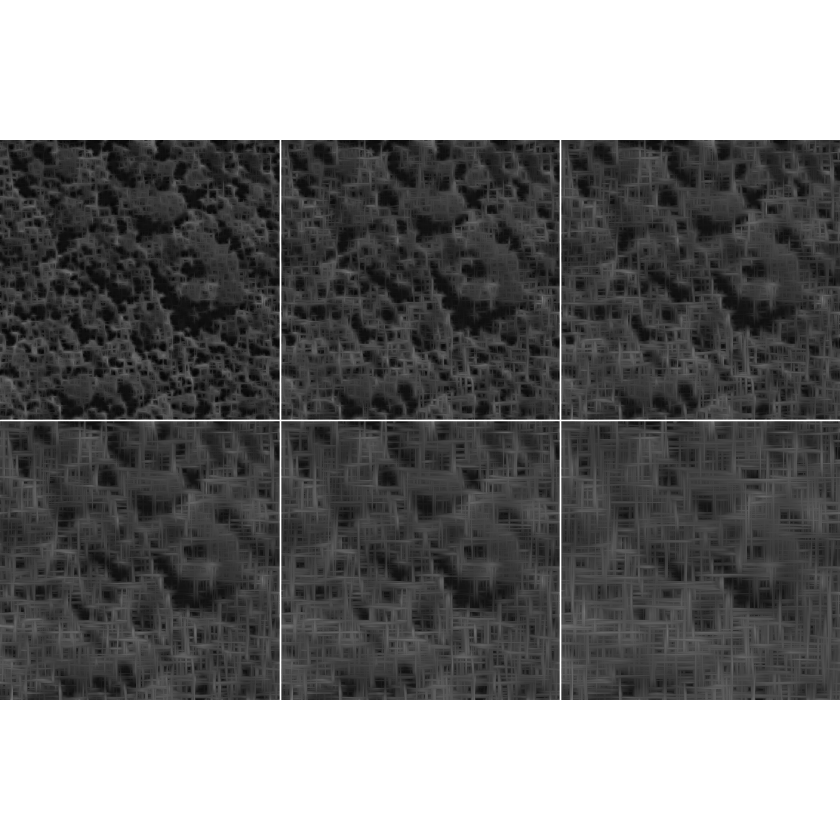
\includegraphics[width=\textwidth]{Imagenes/Resultados script morfologico/GS04.png}
     \hfill
     \caption{Resultado de Rollingball para tamaños de ventana de 6,9,12,15,18 y 24 píxeles}
    \label{Rollingball}
\end{figure}

\begin{figure}
    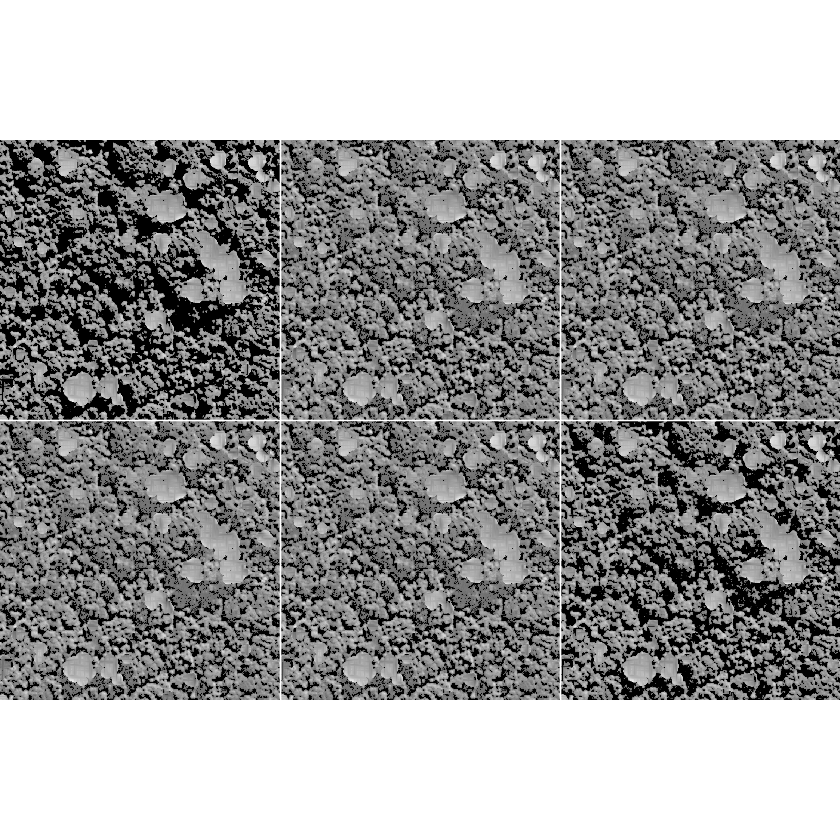
\includegraphics[width=\textwidth]{Imagenes/Resultados script morfologico/GS06.png}
     \hfill
     \caption{Resultado de la segunda selección de objetos oscuros con distintos valores de percentil, 99, 0,1, 1, 10, 50 y 90 }
    \label{segundaoscuros}
\end{figure}

\begin{figure}
    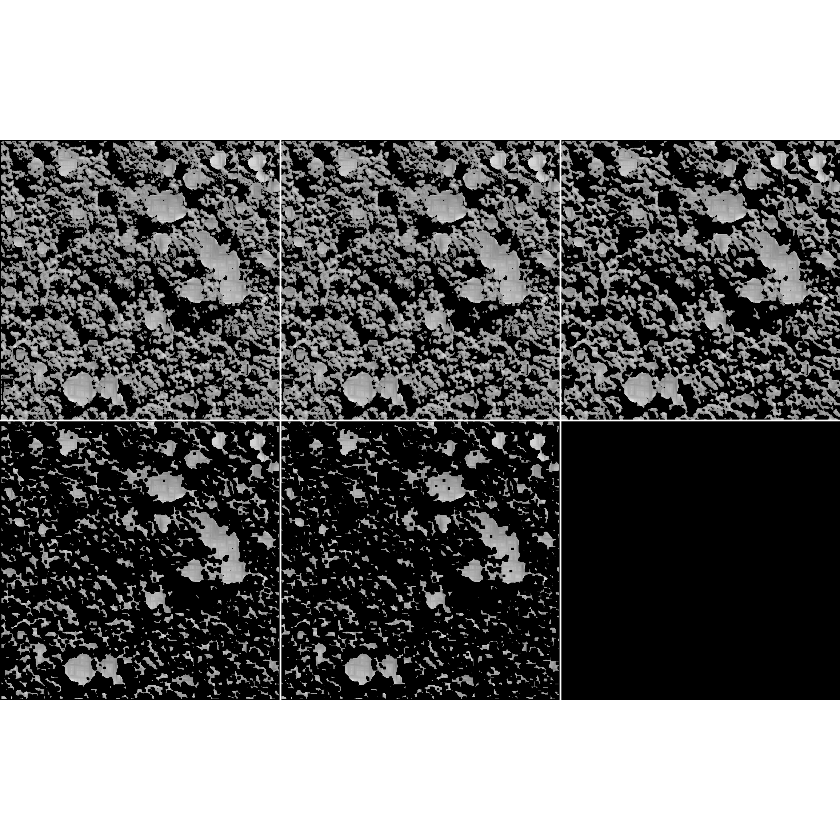
\includegraphics[width=\textwidth]{Imagenes/Resultados script morfologico/GS07.png}
     \hfill
     \caption{Resultado de la búsqueda de pequeños huecos con distintos valores de percentil, 10, 30, 50, 75, 80 y 90 }
    \label{pequenoshuecos}
\end{figure}

\begin{figure}
    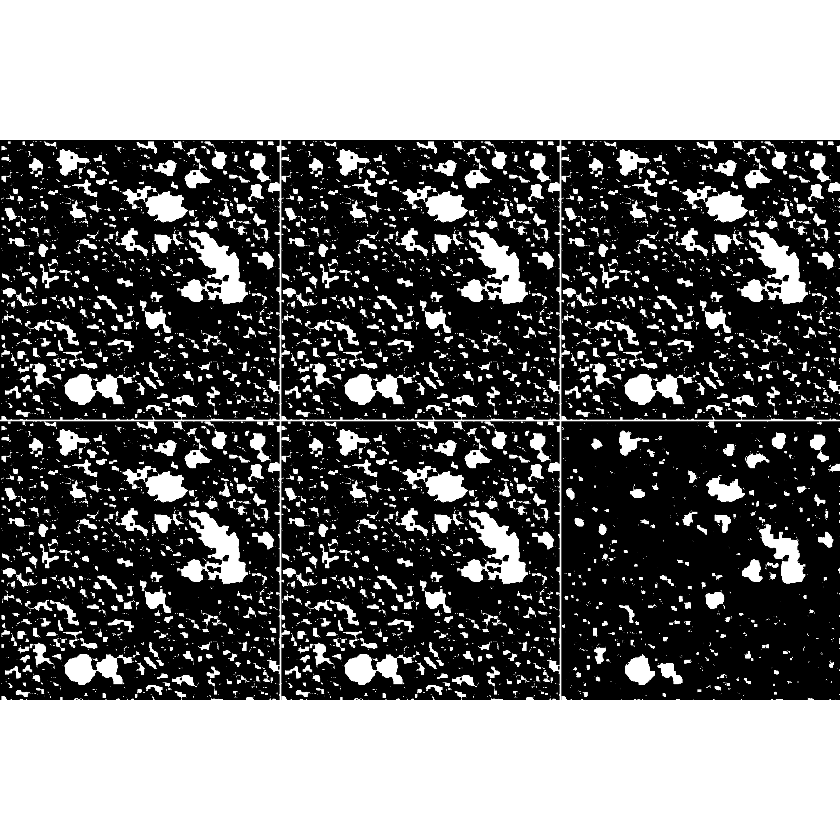
\includegraphics[width=\textwidth]{Imagenes/Resultados script morfologico/GS09.png}
     \hfill
     \caption{Resultado del filtrado con topbottom y binarizado con distintos valores de percentil, 0,1, 1, 10, 20, 50 y 90 }
    \label{topbottom}
\end{figure}
\subsubsection{Evaluación de la influencia de diferentes parámetros en los algoritmos (¿discusión?)}
Se evaluó el desempeño de los algoritmos modificando en un determinado rango el valor de distintos parámetros en cada etapa del procesamiento, para observar en qué modo se ven afectados los resultados. Se procedió a lo que se denomina “Gridsearch”,
estableciendo valores de parámetros en grillas y los correspondientes resultados del procesamiento de las imágenes. En este procedimiento se evidencia la importancia y la vinculación que tienen los parámetros en las diferentes etapas con la resolución espacial de la imagen con la que se trabaja. En tanto en la última etapa se observó que el umbral
que se definió para separar (y por lo tanto binarizar la imagen) las copas segmentadas, en el artículo de referencia sugiere utilizar el umbral del 0,1º percentil, pero al hacer la prueba de Gridsearch con diferentes valores hasta el 90º percentil, resultaba notable que excepto el correspondiente al percentil 90º los demás resultados no eran visiblemente
diferentes.

\color{cyan} %color de texto con 70-80 % o más de avance
\subsection{RESULTADOS HOMOMÓRFICO}
Los resultados de las pruebas se exponen en la Tabla \ref{homomorfico}. Allí se visualiza para distintas imágenes la cantidad de sombras detectadas, y se comparan los resultados de conteo automático con distintos tamaños de ventana, con el método de búsqueda de forma manual. Nótese el cambio de signo para el error medio entre los tamaños de ventana de 25 y de 20 píxeles, indicando que la selección de un tamaño de ventana menor resultará en una mayor 
cantidad de sombras detectadas que la que se obtiene por conteo manual. En cambio un tamaño de ventana mayor podría obviar varias sombras que serían tenidas en cuenta para el conteo manual. De acuerdo con la resolución de las imágenes de prueba, el tamaño de ventana cuadrada de 20 píxeles por lado se correspondería con un área de 100 metros cuadrados.
% Please add the following required packages to your document preamble:
% \usepackage{multirow}
\begin{table}[]
    \centering
    \begin{threeparttable}[b]
        
        \caption{Número de regiones sombreadas obtenidas por conteo manual y por el algoritmo automático de procesamiento homomórfico, como función del tamaño de ventana de exploración}
        % Please add the following required packages to your document preamble:
        \label{tab:resultados_homomorfico}
        \begin{tabular}{ccccccc}
        \hline
        \hline
                  & \textbf{Conteo}  & \multicolumn{5}{c}{\textbf{Tamaño de ventana [píxeles]}}   \\
            \textbf{Imagen}& \textbf{manual}  & \textbf{10 x 10}     & \textbf{15 x 15}     & \textbf{20 x 20 }   & \textbf{25 x 25}    & \textbf{30 x 30 }   \\ \hline
            \textbf{Par1d}  & 5  & 7      & 4      & 1     & 0     & 0     \\
            \textbf{Par2d}  & 2  & 7      & 4      & 1     & 0     & 0     \\
            \textbf{PNI1}   & 14 & 84     & 49     & 31    & 16    & 10    \\
            \textbf{PNI2}   & 14 & 48     & 35     & 20    & 14    & 7     \\
            \textbf{PNI3}   & 32 & 110    & 73     & 48    & 29    & 9     \\
            \textbf{PNI3d}  & 22 & 56     & 42     & 21    & 7     & 0     \\
            \textbf{PS1}    & 6  & 24     & 11     & 5     & 2     & 2     \\ 
            \textbf{YB1}    & 10 & 10     & 5      & 3     & 1     & 1     \\
            \textbf{YB2}    & 9  & 14     & 8      & 4     & 0     & 0     \\
            \textbf{ST1}    & 18 & 40     & 25     & 16    & 7     & 6     \\
            \textbf{ST2}    & 9  & 42     & 30     & 18    & 9     & 7     \\ \hline
            $e_{m}$\tnote{*}    & -  & -27,36 & -13,18 & -2,45 & 5,09  & 9,00  \\ 
            $\sigma^2_{e}$ \tnote{**}   & -  & 637,32  & 216,51 & 62,98 & 25,54 & 49,27 \\
           $\sigma_{e}$ \tnote{***}   & -  & 25,25  & 14,71  & 7,94  & 5,05  & 7,02  \\ \hline \hline
        \end{tabular}
        \begin{tablenotes}
        \tiny{
                \item [*]Error medio.
                \item [**]Varianza.
                \item [***] Desvío estándar.
                }
        \end{tablenotes}
  \end{threeparttable}
\end{table}
       

A los efectos de demostrar el grado de certeza del algoritmo, se comparó con la detección manual, variando el tamaño de la ventana de enmascaramiento. Se comprobó que eligiendo un tamaño de ventana de enmascaramiento igual a 20 por 20 píxeles se obtenía un acercamiento al criterio de selección manual.
En el proceso de binarización, se definió como umbral que correspondía a un valor de intensidad por encima del cual se trataba de sombras. En este caso el valor de intensidad fue de 0,75 en valores de intensidad de píxeles normalizados.
Para la selección de sombras binarizadas se recorrió la matriz de la imagen con una ventana de inspección que abarcaba 25 píxeles por lado, de modo que se evalúa un conjunto de 625 píxeles. Se estableció un umbral de 0,45 para clasificar las sombras, de modo que los recintos de píxeles blancos que superaban ese umbral eran catalogados como sombras de árboles grandes.
A los efectos de mostrar el funcionamiento del método de búsqueda y conteo de sombras, se exponen las figuras \ref{sombratorogris}, \ref{mascaraST} y \ref{seleccionadaST} en las que se visualizan la imagen satelital en escala de grises de una porción de la reserva privada Sombra de Toro, ubicada en el norte de la provincia de Misiones, la imagen binarizada luego del filtrado homomórfico y las sombras seleccionadas, respectivamente.

\begin{figure}
    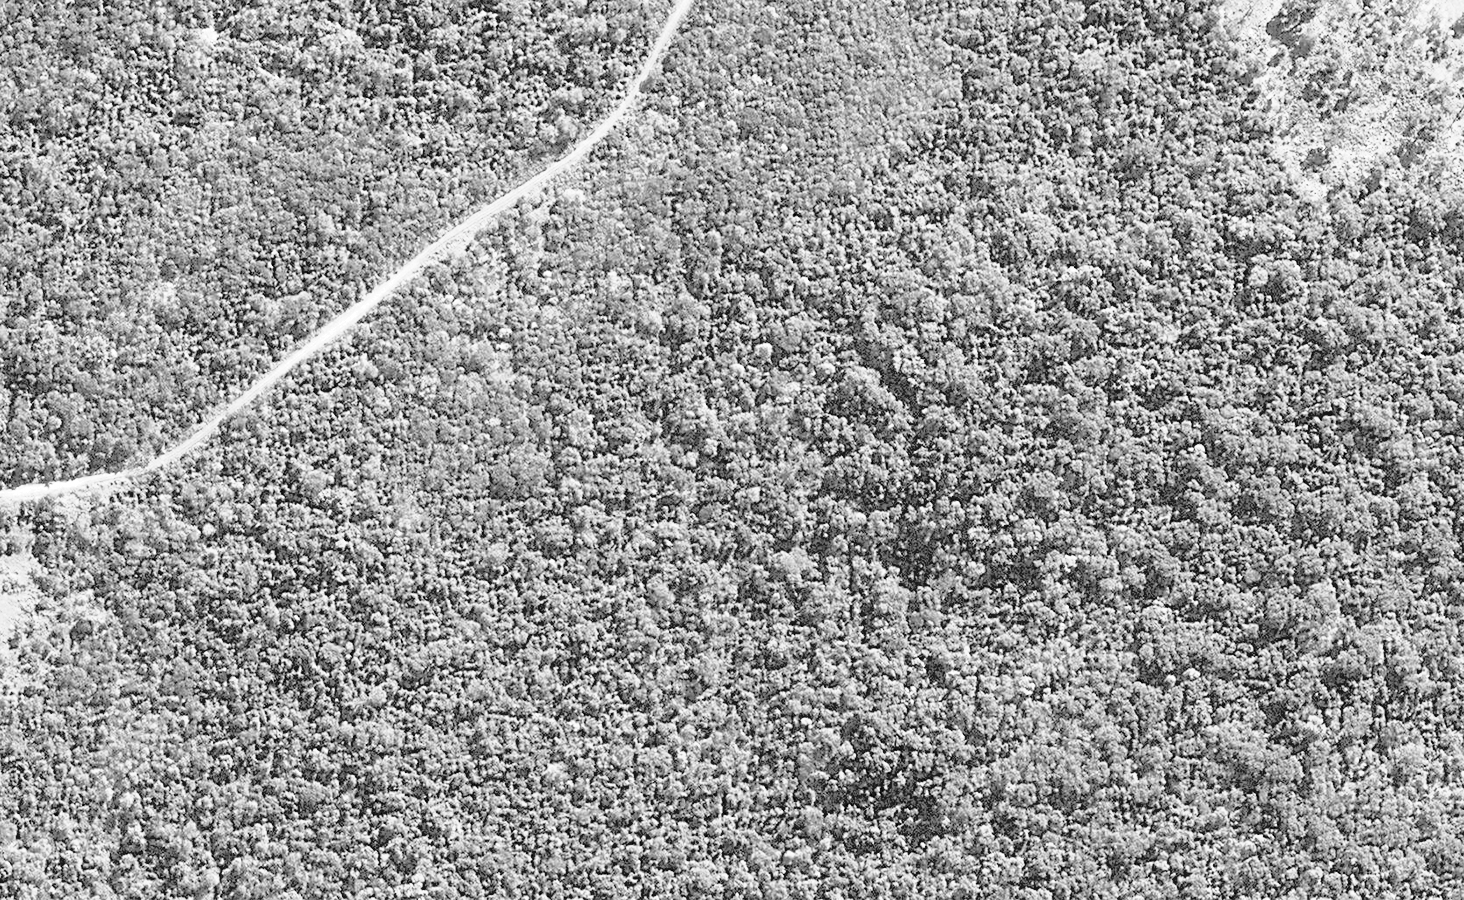
\includegraphics[width=\textwidth]{Imagenes/Homomorfico/ST2.jpg}
     \hfill
     \caption{Imagen aérea (satelital) de reserva privada Sombra de Toro, en escala de grises}
    \label{sombratorogris}
\end{figure}

\begin{figure}
    
\includegraphics[width=\textwidth]{Imagenes/Homomorfico/ST2_bin.jpg}
     \hfill
     \caption{Máscara binaria}
    \label{mascaraST}
\end{figure}

\begin{figure}
    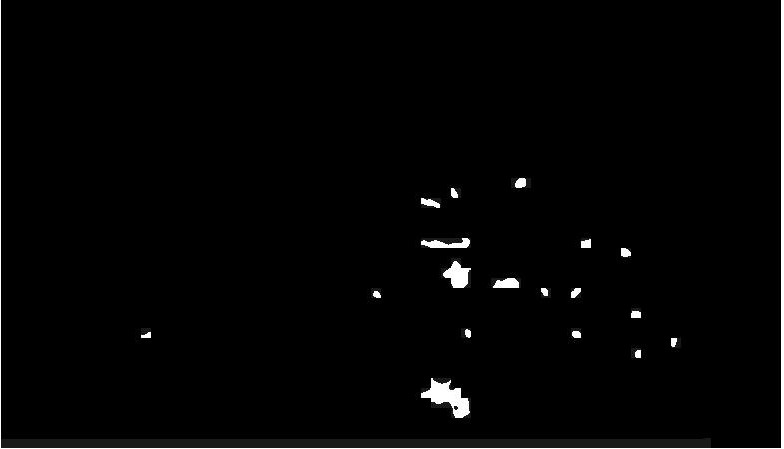
\includegraphics[width=\textwidth]{Imagenes/Homomorfico/ST2_masked.jpg}
     \hfill
     \caption{Sombras seleccionadas}
    \label{seleccionadaST}
\end{figure}

\color{cyan} %color de texto con 70-80 % o más de avance
\subsection{RESULTADOS IIC} \label{Resultados}
Un total de diecinueve imágenes aéreas de selva fueron consideradas para realizar el análisis. Dos de ellas representativas de los diferentes escenarios que fueron cubiertos, se muestran en las figuras \ref{calle} y \ref{tupido}. La figura \ref{calle} muestra una imagen en la que unas pocas copas de árboles se distribuyen por el área capturada, mientras que en la \ref{tupido} el dosel cubre prácticamente toda el área. La delineación manual de las sombras fue realizada como se describe en el apartado de \ref{Metodología}
Dos ejemplos de máscaras manuales se muestran en figuras \ref{contorno1} y \ref{contorno2}, con trazo rojo bordeando las regiones sombreadas. La figura \ref{superposicion} muestra el solapamiento de la máscara manual (en rojo) con la automática (en azul). En la figura \ref{p60} el valor de umbral para la máscara binaria se toma del 60º percentil de la distribución de frecuencias, mientras que en la figura \ref{p85} el valor de umbral es tomado del 85º percentil.

\begin{figure}
    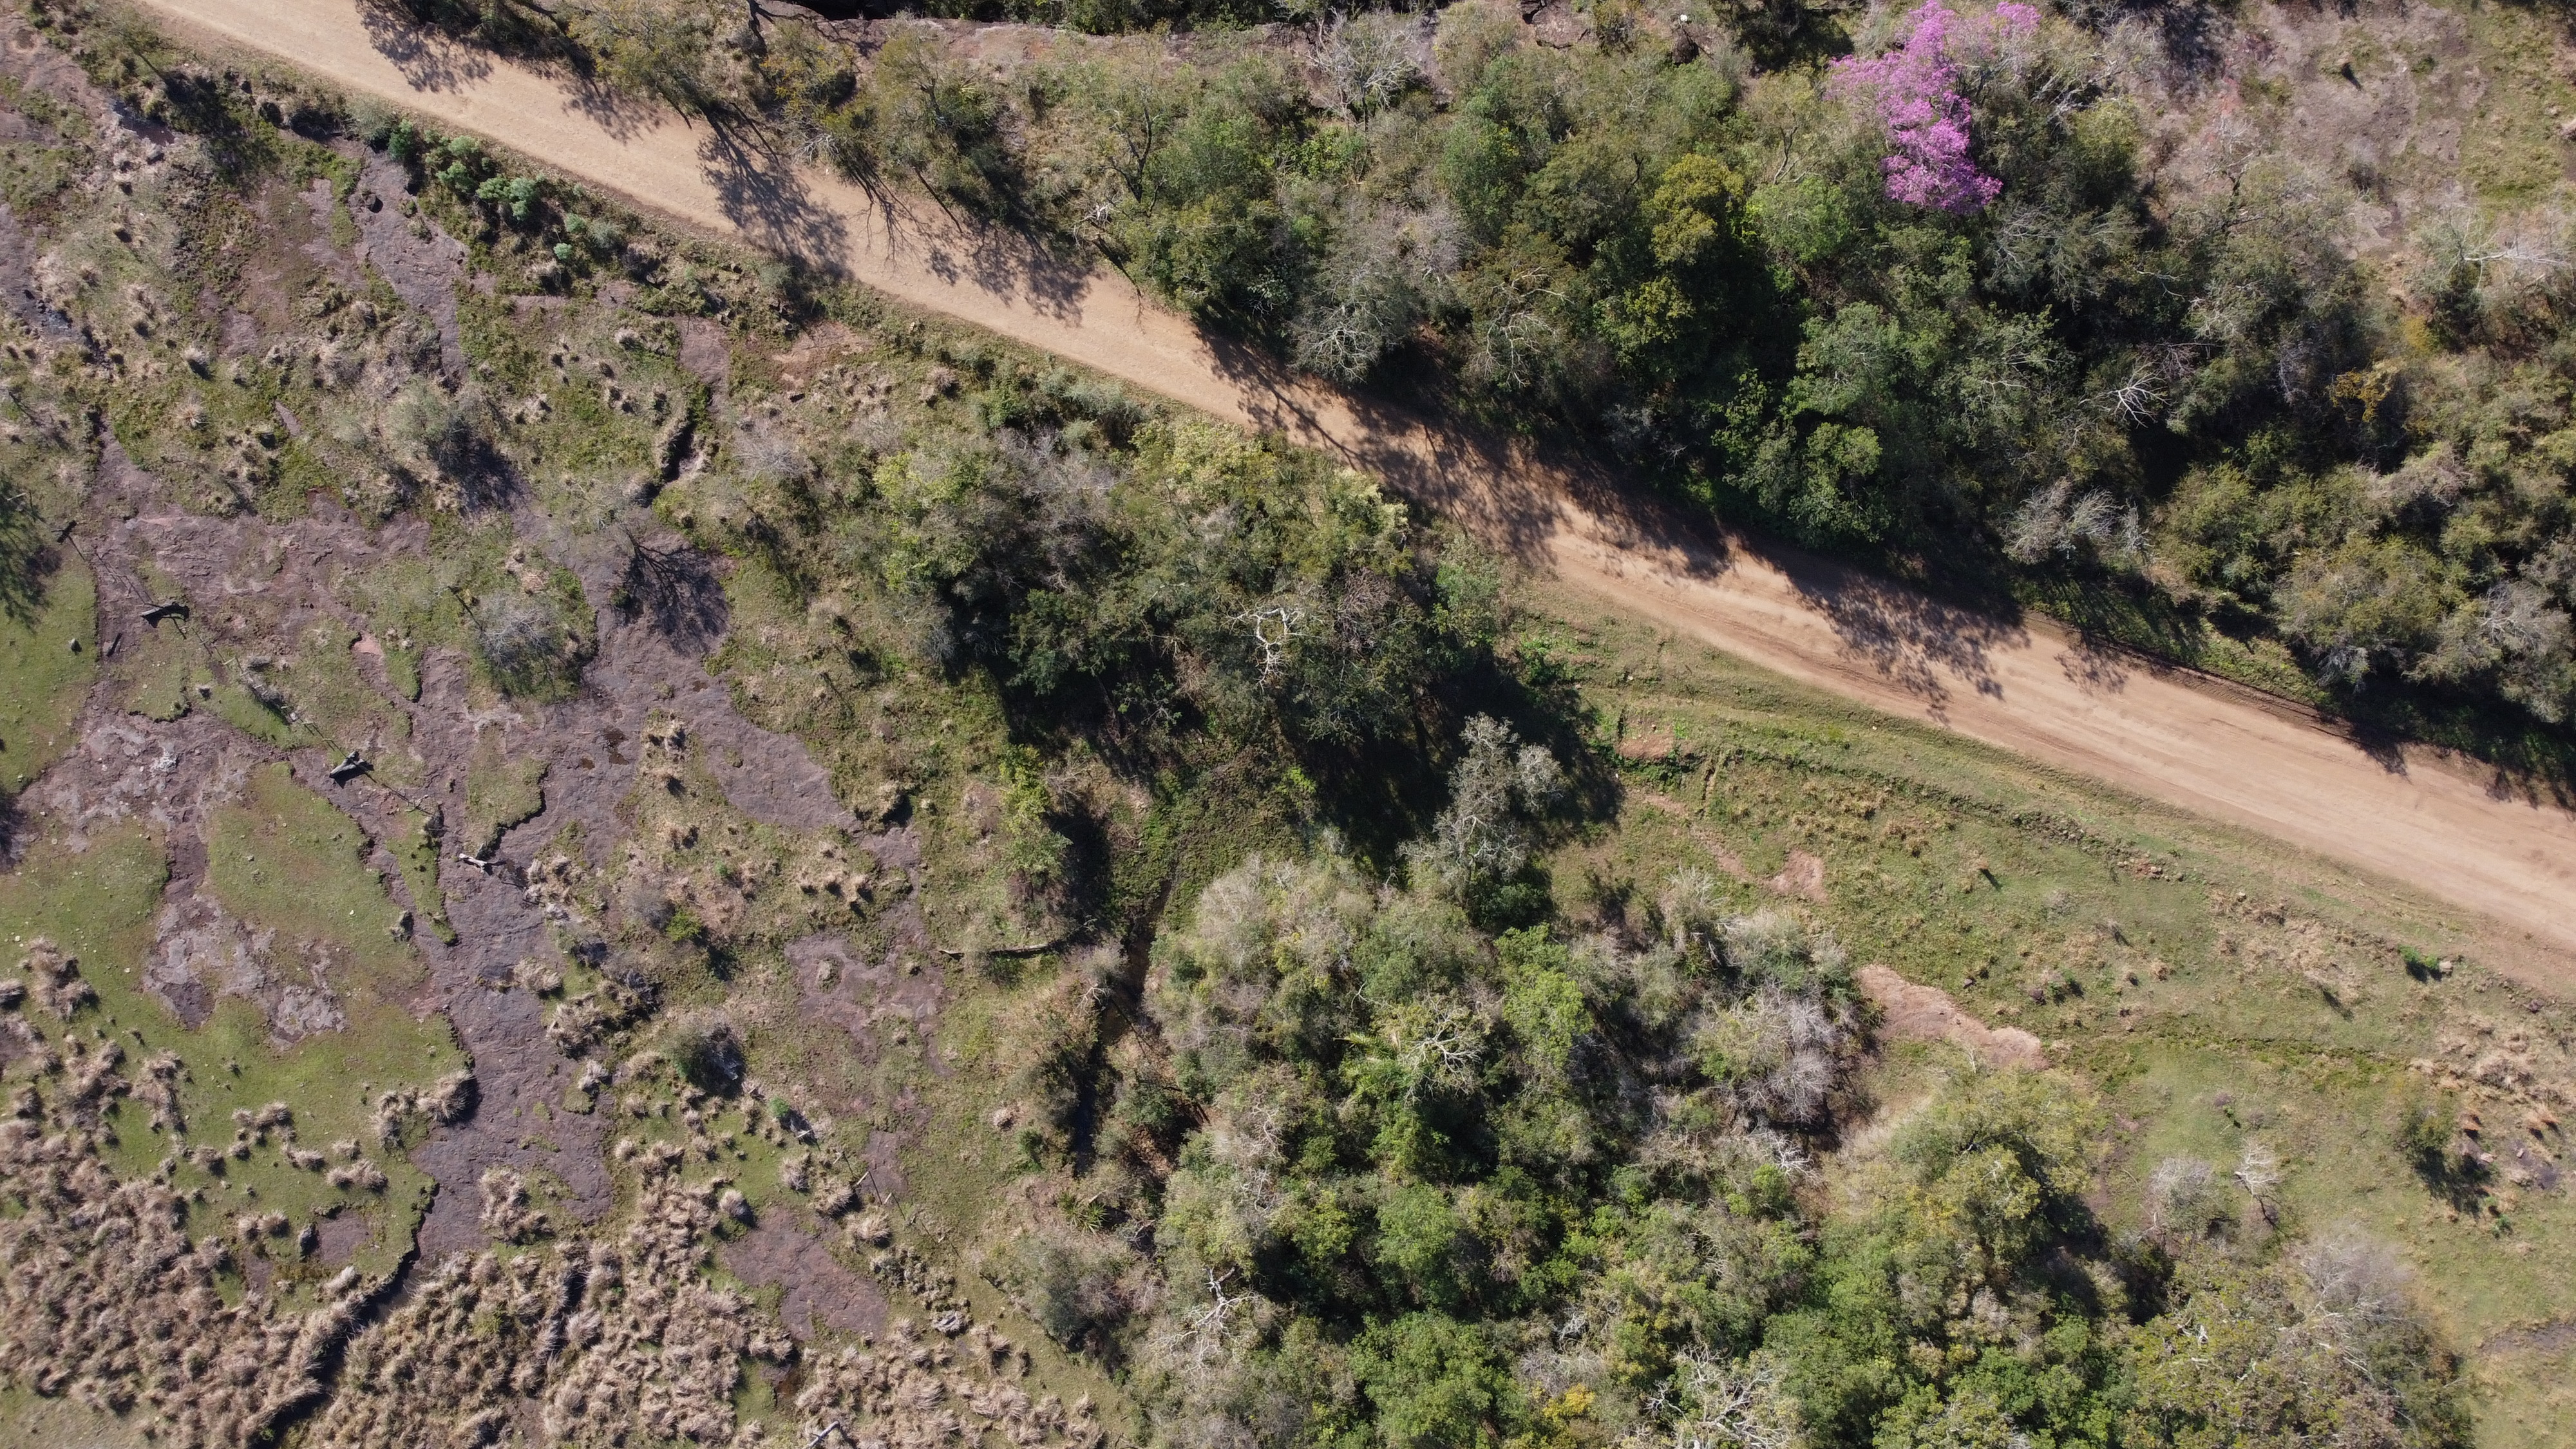
\includegraphics[width=\textwidth]{Imagenes/street.jpg}
     \hfill
     \caption{Escena capturada con pocos árboles}
    \label{calle}
\end{figure}

\begin{figure}
    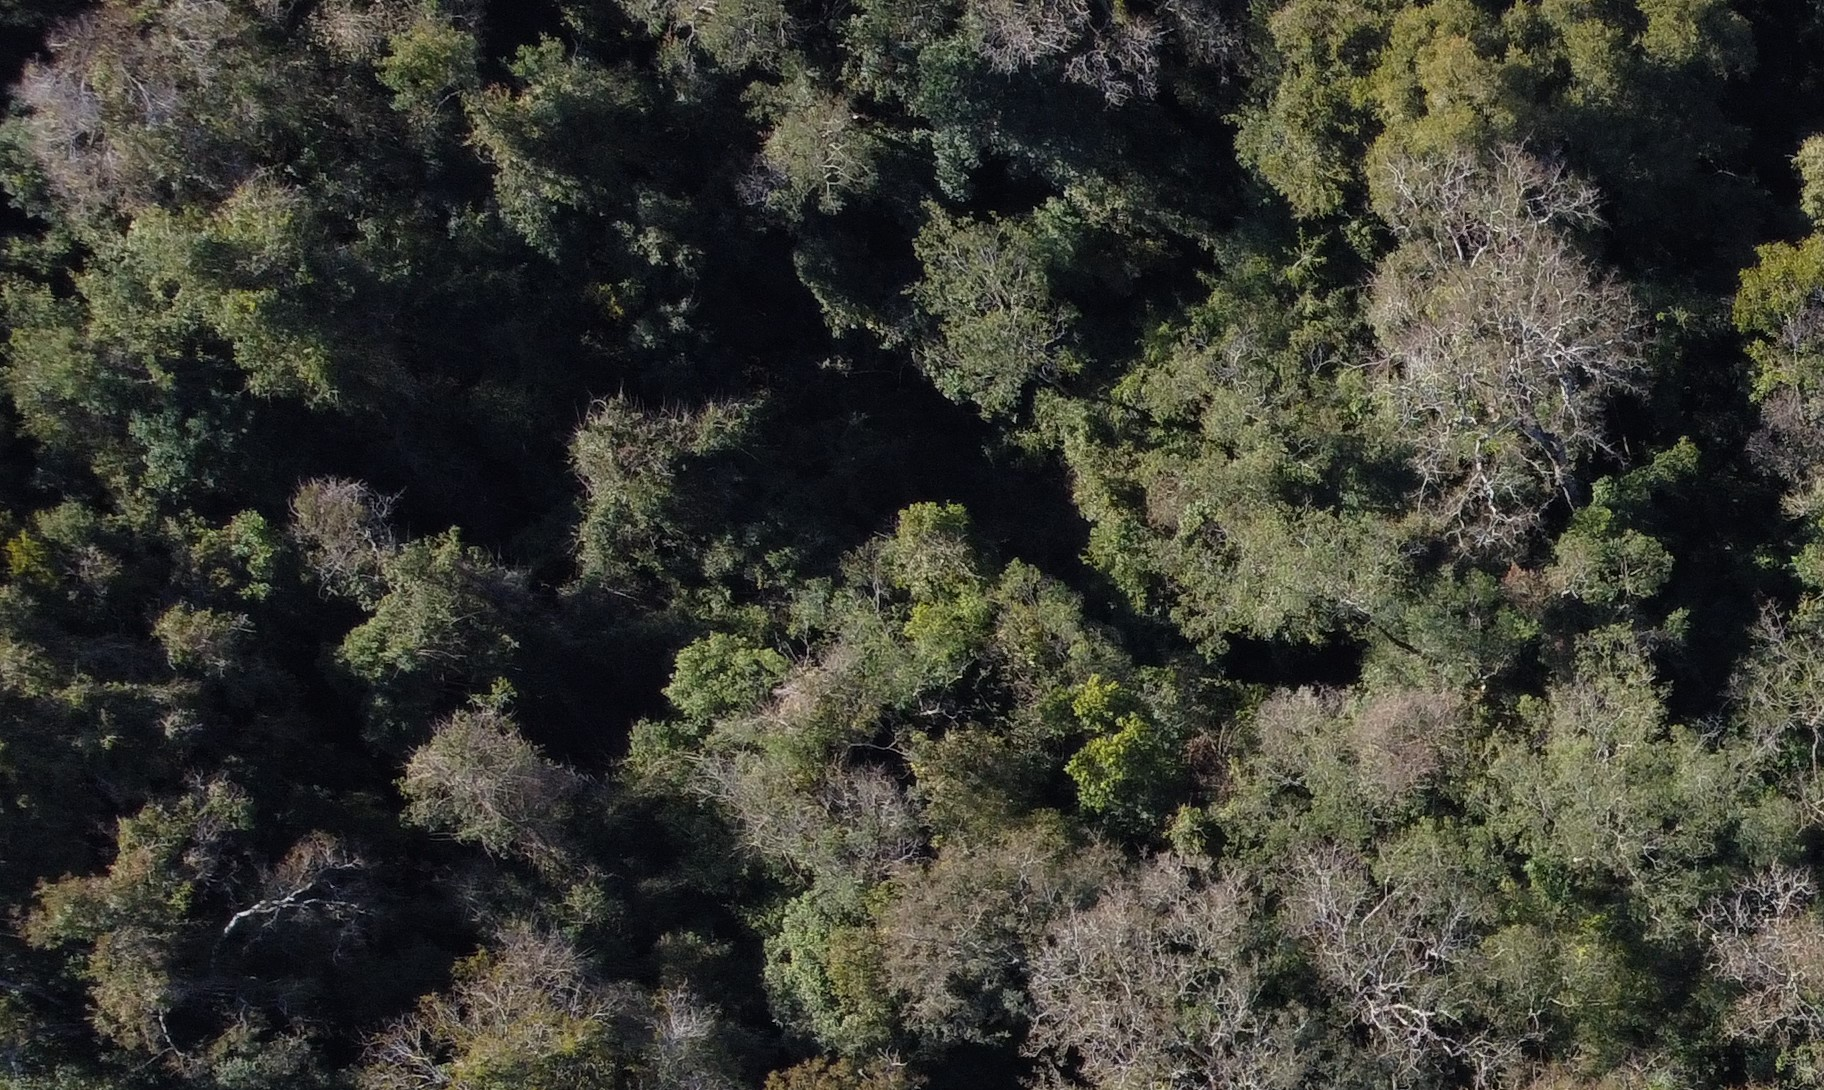
\includegraphics[width=\textwidth]{Imagenes/dense canopy.jpg}
     \hfill
     \caption{Escena capturada con dosel tupido}
    \label{tupido}
\end{figure}


\begin{figure}
    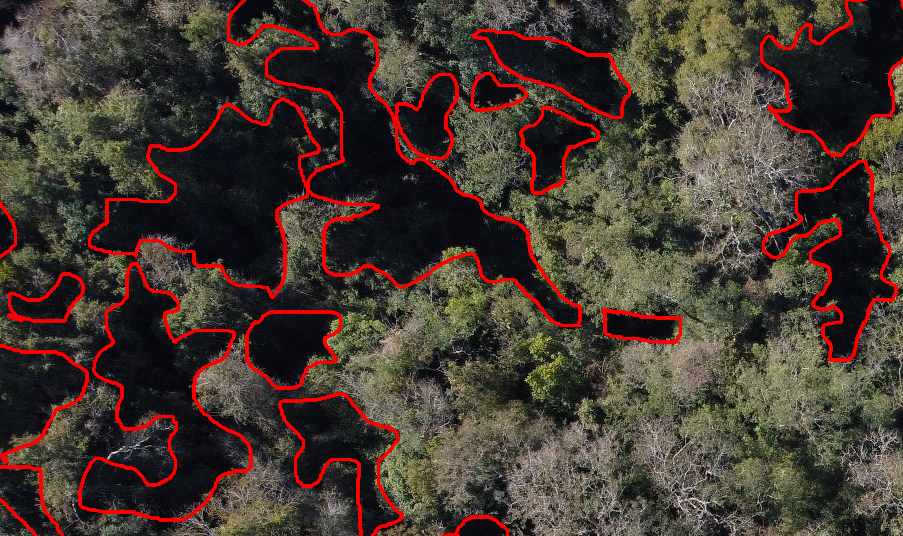
\includegraphics[width=\textwidth]{Imagenes/contours.png}
     \hfill
     \caption{Contornos de sombras en dosel tupido}
    \label{contorno1}
\end{figure}

\begin{figure}
    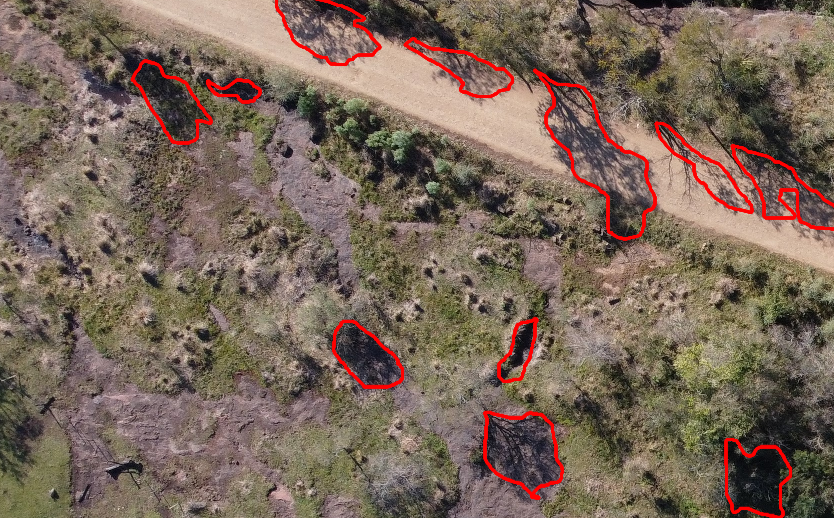
\includegraphics[width=\textwidth]{Imagenes/contours2.png}
     \hfill
     \caption{Contorno de sombras en imagen con pocos árboles}
    \label{contorno2}
\end{figure}

\begin{figure}
     \centering
     \begin{subfigure}[b]{0.5\textwidth}
         \centering
         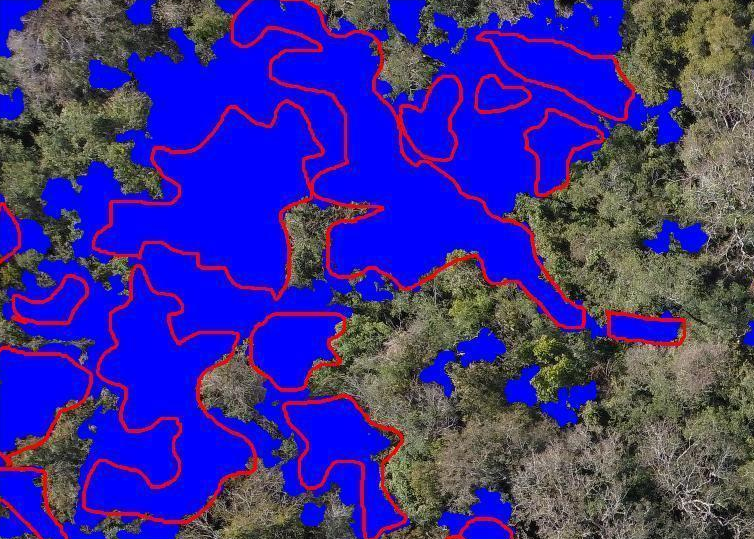
\includegraphics[width=\textwidth]{Imagenes/superposition of masks.png}
         \caption{Percentil 60º}
         \label{p60}
     \end{subfigure}
     \hfill
     
     \begin{subfigure}[b]{0.5\textwidth}
         \centering
         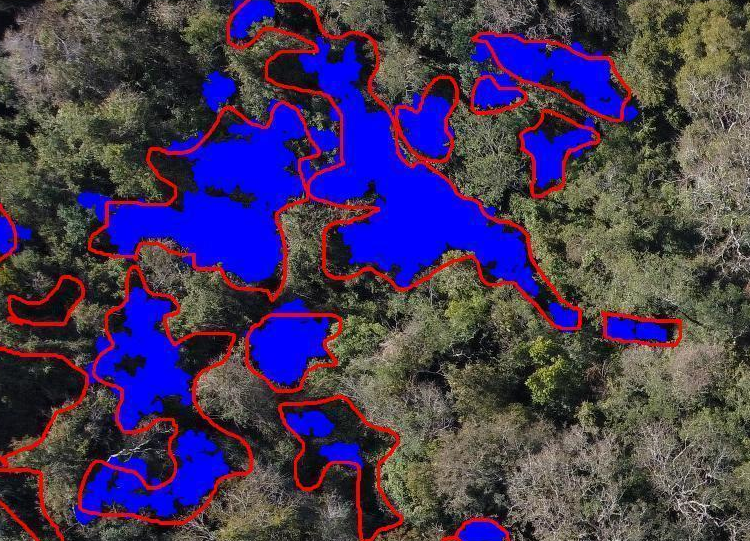
\includegraphics[width=\textwidth]{Imagenes/superposition of masks 2.png}
         \caption{Percentil 85º}
         \label{p85}
     \end{subfigure}
        \caption{Superposición de máscaras atuomática y manual}
        \label{superposicion}
\end{figure}

\begin{figure}
    \centering
  \begin{subfigure}[b]{0.3\textwidth}
    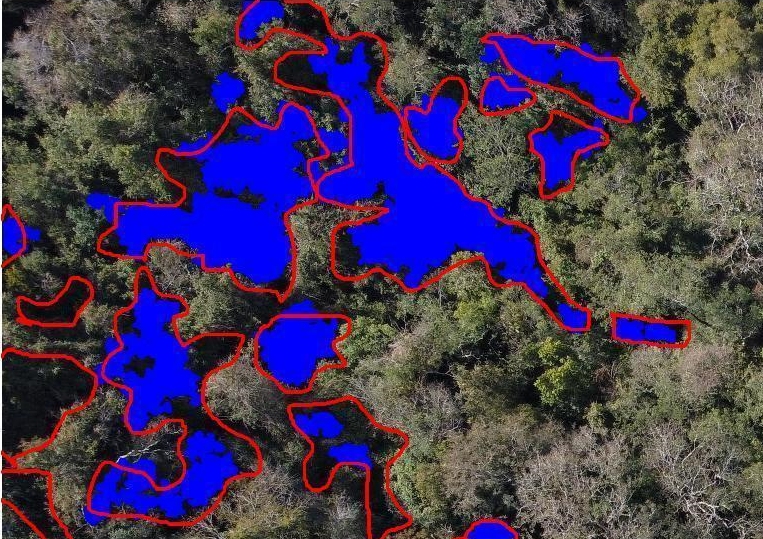
\includegraphics[width=\textwidth]{Imagenes/blue minus red 85.png}
     \hfill
     \caption{\textpsi\textsubscript{BR}}
    \label{azulrojo}
 \end{subfigure}

 \begin{subfigure}[b]{0.3\textwidth}
    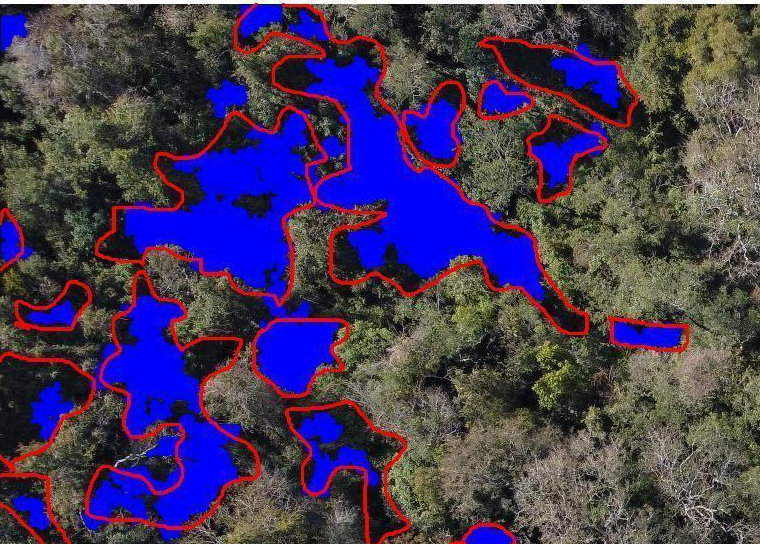
\includegraphics[width=\textwidth]{Imagenes/blue minus green 85.png}
     \hfill
     \caption{\textpsi\textsubscript{BG}}
    \label{azulverde}
 \end{subfigure}

 \begin{subfigure}[b]{0.3\textwidth}
    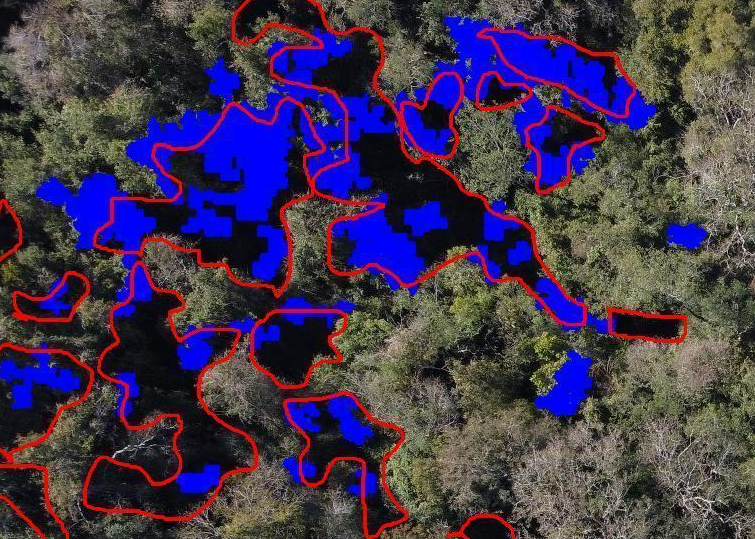
\includegraphics[width=\textwidth]{Imagenes/green minus red 85.png}
     \hfill
     \caption{\textpsi\textsubscript{GR}}
    \label{verderojo}
 \end{subfigure}
 \caption{Superposición de máscaras atuomática y manual}
        \label{p85BRBGGR}
\end{figure}

\paragraph{Influencia del valor de percentil y del índice invariante de color}

La figura \ref{azulrojo}, \ref{azulverde} y \ref{verderojo} muestra para la misma escena, diferentes máscaras automáticas obtenidas con diferentes configuraciones de la ecuación \ref{invariante de color}, usando tres diferentes combinaciones de canales de dos colores. La figura \ref{azulrojo} corresponde a la máscara obtenida usando la diferencia entre el canal azul menos el canal rojo $\Psi_{BR}$, la figura \ref{azulverde} usando la diferencia entre el canal azul menos el canal verde $\Psi_{BG}$ y la figura \ref{verderojo} usando la diferencia entre el canal verde menos el canal rojo $\Psi_{GR}$. En todos los casos el valor de umbral fue tomado del 85º percentil de la distribución de frecuencia. El análisis de las figuras \ref{azulrojo} a \ref{verderojo} muestra que, aplicando la ecuación \ref{eq1} usando ya sea la combinación de canales azul con verde $\Psi_{BG}$ o azul con rojo $\Psi_{BR}$  las máscaras automáticas resultantes para un mismo valor de percentil son de área mayor que las que corresponden al índice calculado con la diferencia entre canal verde y rojo $\Psi_{GR}$, lo que resulta en valores de QI más altos para $\Psi_{BR}$ y $\Psi_{BG}$ que para $\Psi_{GR}$. La comparación entre las distintas influencias del valor de percentil puede observarse en la figura \ref{curvas_QI}, donde resulta evidente que $QI_1$ es el más alto en el percentil bajo 60º y $QI_2$ es el más alto para el percentil alto 95º. Por otro lado el índice $QI_3$ se asemeja a una curva convexa, con valores similares a $QI_1$ para el percentil 60º y similares a $QI_2$ para el percentil 95º, cuyo valor máximo en la curva corresponde al 85º percentil. Un comportamiento similar se observa para los otros índices invariantes de color $\Psi_{BG}$ y $\Psi_{GR}$. La similitud entre QI1 y QI2 en el percentil más bajo se debe al hecho de que la máscara automática selecciona un área de sombra que resulta preponderante en la operación de unión binaria en el denominador de la ecuación \ref{qi3} en el caso de $QI_3$.
Por otro lado, el índice $QI_3$ se aproxima a $QI_1$ cuando la máscara automática selecciona un área pequeña de sombra, por lo tanto la selección manual de sombra resulta dominante en la operación de unión de máscaras en el denominador de la ecuación \ref{qi3}.
Al maximizar la intersección, se asegura la coincidencia entre las máscaras manual y automática, pero podría excederse en la máscara automática. Luego, al minimizar la unión, se puede controlar el tamaño pleno de la máscara automática. Un punto óptimo es el caso en el que el índice $QI_3$ alcanza el máximo valor. A pesar de la dispersión de los datos (ver figura \ref{curvas_QI}), se puede analizar los valores medios de los índices de calidad QI para los tres casos considerados (ver figuras \ref{psiBR}, \ref{psiBG}, \ref{psiGR}). Se observa que el valor que corresponde al 85º percentil de la distribución de frecuencia del índice invariante de color es el óptimo, ya que corresponde a un máximo del índice $QI_3$.
En el análisis e la figura \ref{}, se observan grandes similitudes, donde se grafican las relaciones entre los tres índices de calidad propuestos y un índice adicional definido como la diferencia entre el valor máximo y el mínimo entre los tres índices en función del valor de percentil usado para calcular el umbral de la máscara binaria automática. En los tres casos se detecta un valor mínimo para la curva que corresponde al índice adicional, es decir el rango (max - min), y este valor mínimo corresponde al percentil 85º. Además para los casos que usan sendas combinaciones en la ecuación \ref{eq1} resta de canal azul menos rojo y azul menos verde, la curva del índice $QI_3$ alcanza un valor máximo en el que corresponde al 85º percentil, mientras que este punto máximo no se hace evidente para el caso de de la combinación verde menos rojo. Por lo tanto de los cuatro índices que fueron analizados, el más conveniente es el $QI_3$, que exhibe un valor óptimo de percentil más preciso por medio del mínimo en la curva, y en los tres casos de combinaciones de canales es coincidente.

\paragraph{Influencia del filtro de mediana en la detección automática de sombras}

La figura \ref{}, \ref{} y \ref{} muestra cómo los índices que son obtenidos por las ecuaciones \ref{qi5} a \ref{qi7} son afectados por la implementación del filtro de mediana a cada imagen. En el caso del filtro de 3 x 3 píxeles, que tiene menor incidencia en los índices, los índices de calidad tienen valores mayores al 85\% para todas las imágenes. El peor desempeño lo tiene el filtro de 12 x 12, cuyo resultado comparado con la máscara automática obtenida sin filtro arrojaba una coincidencia de poco más que el 70\%.

\paragraph{Evaluación humana de máscaras automáticas de sombra}

En este trabajo los resultados del algoritmo se comparan con la selección manual llevada a cabo por expertos. Partiendo de que no hay una base de certeza absoluta (los expertos son personas humanas y por lo tanto proclives a errores de omisión o comisión), existe una limitación en el índice de calidad que se basa en este aspecto. El criterio para la selección manual de parte de los expertos depende de su particular percepción de la imagen, variando según el contexto. Por otro lado el algoritmo se basa en el cálculo de un índice y la definición de un valor umbral, obtenido de una serie de experimentos con imágenes de un determinado tipo. En otros contextos con otro tipo de imágenes el valor de umbral no sería el mismo, incluso la combinación de bandas usadas en la ecuación \ref{invariante de color} para obtener el índice sería diferente.
Luego de generar un conjunto de máscaras correspondientes a cada uno de los seis percentiles usando los tres índices invariantes de color de las ecuaciones \ref{psibr} a \ref{psigr} para las 19 imágenes seleccionadas, las 342 máscaras resultantes fueron comparadas con las obtenidas manualmente. Superponiendo ambas, la máscara automática y la manual sobre la imagen original, se evaluó la calidad de las similitudes mutuas, asignando un calificativo en tres niveles, "bueno", "regular" y "malo". Los resultados se muestran en la tabla \ref{tablita} y en la figura \ref{}. Tal como se puede apreciar, para los tres índices invariantes de color se puede observar un mínimo en el nivel "malo" alrededor del percentil 90º. Para los niveles "regular" y "bueno", sin embargo, el mínimo no es tan claro, lo cual puede ser atribuido a cierta subjetividad de los observadores expertos.

%%%%%%%%%%%%%%%%%%%%%%%%%%%%%%%%%%%%%%%%% TABLA %%%%%%%%%%%%%%%%%%%%%%%%%%%%%%%%%%%%%%%%%%%%%%%%%%%%%%%%%
\begin{table}[H]
    \centering
    \caption{Evaluation of the superposition of both masks. the manual and the automatic. carried on by the group of experts}
    \begin{tabular}{|c|c|c|c|c|c|c|c|}
       \hline
        COLOR INVARIANT INDEX & \multicolumn{6}{ |c|}{\textpsi \textsubscript{BR}}\\%\multicolumn{6}{ }{ |c|} \\
        \hline
        PERCENTILE & 60 & 70 & 80 & 85 & 90 & 95\\
        \hline
        GOOD & 0.0 & 0.0 & 4.5 & 15.8 & 20.5 & 0.0\\
        \hline
        REGULAR & 0.0 & 4.5 & 27.3 & 21.1 & 54.5 & 57.9\\
        \hline
        BAD & 100.0 & 95.5 & 68.2 & 63.2 & 25.0 & 42.1\\
        \hline
        COLOR INVARIANT INDEX & \multicolumn{6}{ |c|}{\textpsi \textsubscript{BG}}\\
        \hline
        PERCENTILE & 60 & 70 & 80 & 85 & 90 & 95\\
        \hline
        GOOD & 0.0 & 0.0 & 0.0 & 5.3 & 5.3 & 5.3\\
        \hline
        REGULAR & 0.0 & 5.3 & 10.5 & 15.8 & 42.1 & 21.1\\
        \hline
        BAD & 100.0 & 94.7 & 89.5 & 78.9 & 52.6 & 73.7\\
        \hline
        COLOR INVARIANT INDEX & \multicolumn{6}{|c|}{ \textpsi \textsubscript{GR}}\\
        \hline
        PERCENTILE & 60 & 70 & 80 & 85 & 90 & 95\\
        \hline
        GOOD & 0.0 & 0.0 & 0.0 & 0.0 & 0.0 & 0.0\\
        \hline
        REGULAR & 0.0 & 0.0 & 0.0 & 0.0 & 15.8 & 15.8\\
        \hline
        BAD & 100.0 & 100.0 & 100.0 & 100.0 & 84.2 & 84.2\\
        \hline
    \end{tabular}
    \\
    \raggedleft
    \label{tablita}
\end{table}
%%%%%%%%%%%%%%%%%%%%%%%%%%%%%%%%%%%%%%%%%%%%%%%%%%%%%%%%%%%%%%%%%%%%%%%%%%%%%%%%%%%%%%%%%%%%%%%%%%%%%%%%%


\begin{figure}
         \centering
         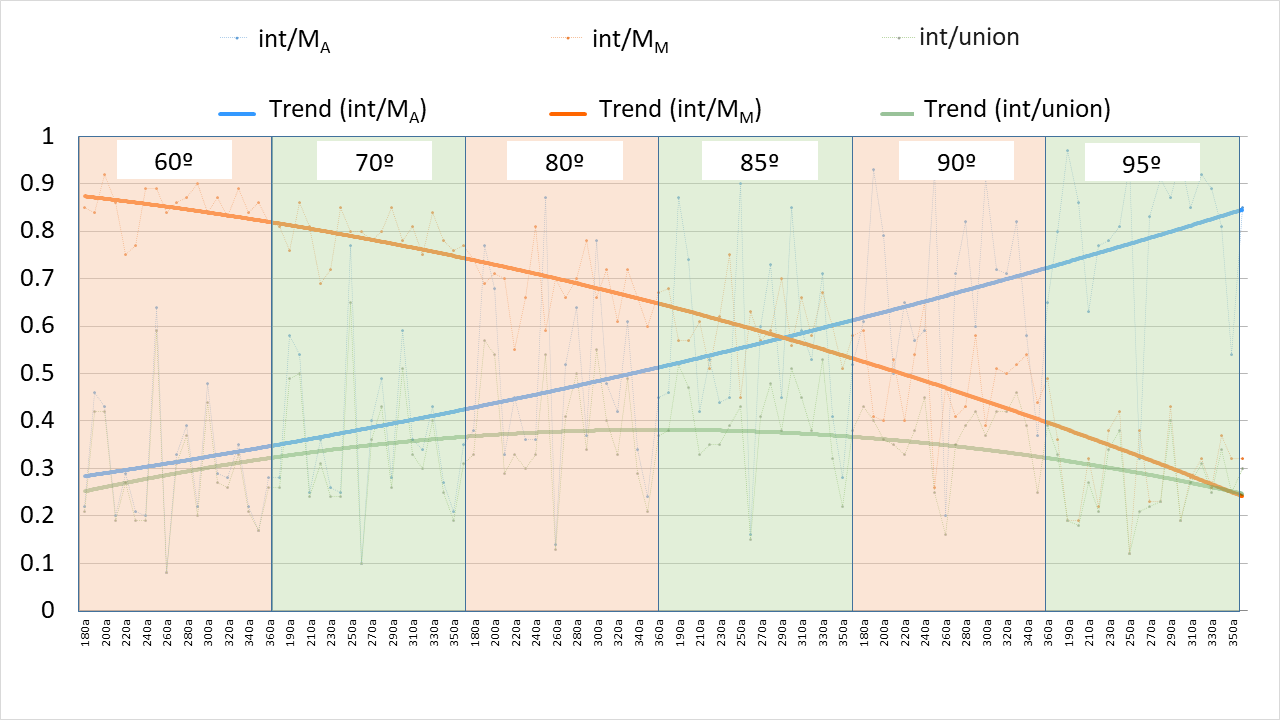
\includegraphics[width=\textwidth]{Imagenes/grafico.png}
         \hfill
         \caption{Curvas índice de calidad}
        \label{curvas_QI}
\end{figure}

%%%%%%%%%%%%%%%%%%%%%%%%%%%%%%%%%%%%%%%%%%%%%%
\begin{figure}
     \centering
     \begin{subfigure}[b]{0.3\textwidth}
         \centering
         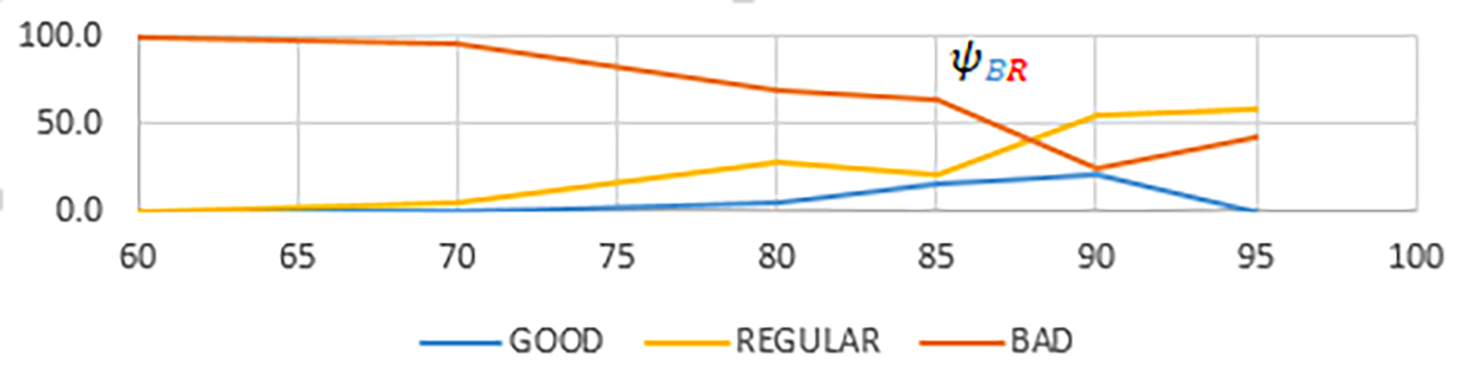
\includegraphics[width=\textwidth]{Imagenes/psiBR.png}
         \caption{\textpsi \textsubscript{BR}}
         \label{psiBR}
     \end{subfigure}
     \hfill
     \begin{subfigure}[b]{0.3\textwidth}
         \centering
         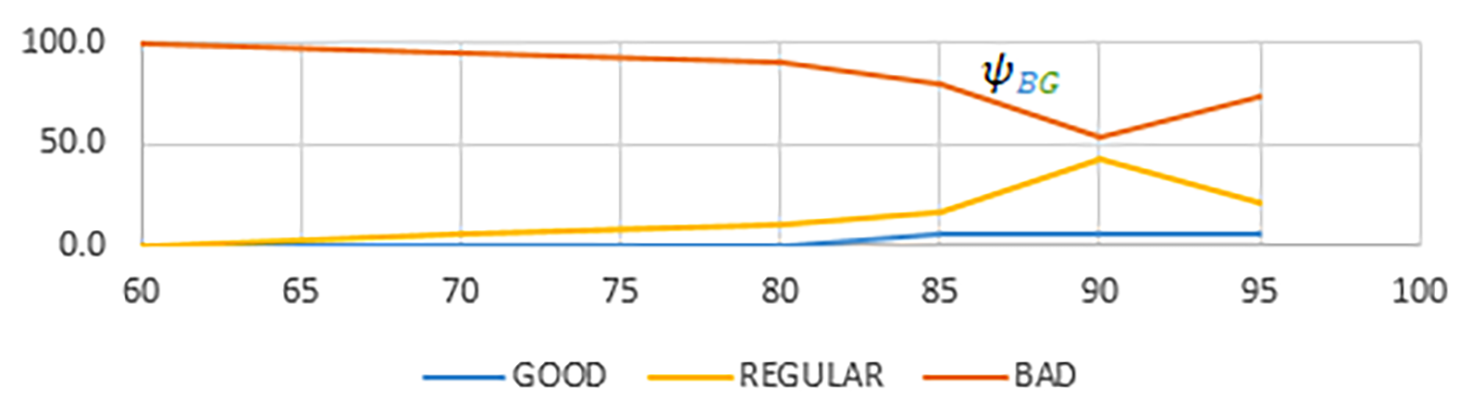
\includegraphics[width=\textwidth]{Imagenes/psiBG.png}
         \caption{\textpsi \textsubscript{BG}}
         \label{psiBG}
     \end{subfigure}
     \hfill
     \begin{subfigure}[b]{0.3\textwidth}
         \centering
         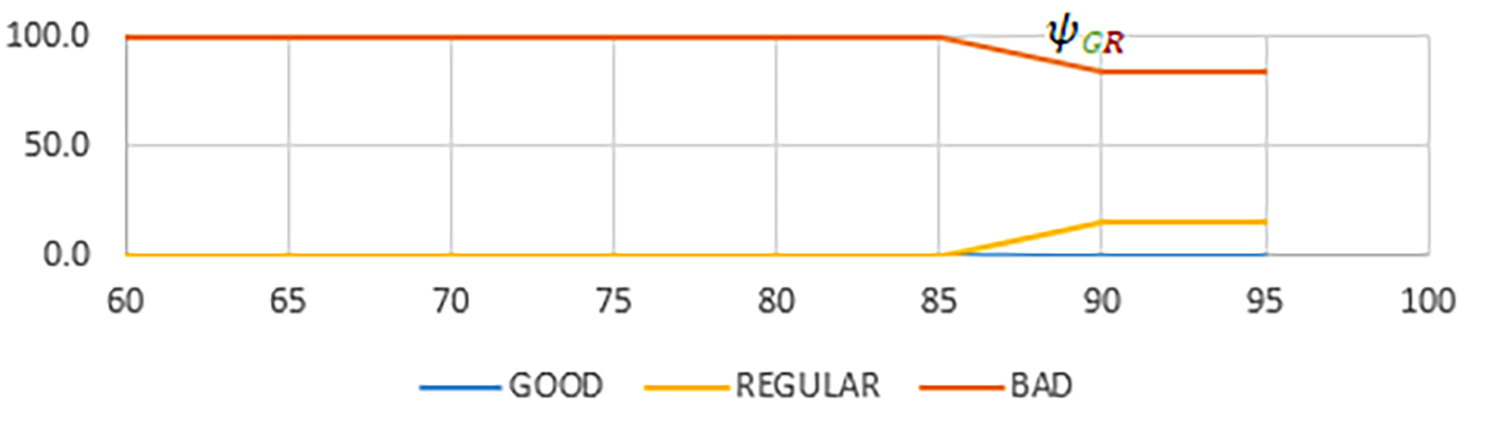
\includegraphics[width=\textwidth]{Imagenes/psiGR.png}
         \caption{\textpsi \textsubscript{GR}}
         \label{psiGR}
     \end{subfigure}
        \caption{Qualification of overlapping of both, manual and automatic masks by human experts}
        \label{humanscoring}
\end{figure}
\subsubsection{Validación IIC} \label{Validacion}
Superponiendo a una imagen las dos máscaras, una obtenida en forma manual y otra en forma automática, tres expertos realizaron un análisis, calificando el grado de ajuste entre ambas máscaras como "bueno", "regular" o "malo". Este procedimiento fue aplicado a cada una de las 19 imágenes analizadas, de modo que se obtuvieron 19 máscaras automáticas por medio del algoritmo para ser comparadas con las respectivas máscaras obtenidas en forma manual. Las superposiciones calificadas como "buenas" o "regulares" son usadas para seleccionar la mejor máscara automática. Un procedimiento similar se siguió para evaluar el filtrado de la imagen.

\color{black} 
\subsection{C3-Filtros de texturas (probados con fantomas)}
Mediante el filtrado por textura puede implementarse una segmentación o clasificación en imágenes. Se hicieron varias pruebas con imágenes simuladas (cuadrados y rombos)
\subsection{C4-Mapas autoorganizados (clasificación no supervisada)}
\subsection{C5-IIC: Análisis de efecto de bandas utilizadas (sombras)}
Informe 1
Se realizaron pruebas del algoritmo sobre distintas imágenes que contienen sombra para ver su desempeño en la selección automática de sombras. Para todos los casos se aplicó para definir el umbral de binarización el correspondiente al percentil 85 de la distribución de frecuencias del índice invariante de color calculado por la ecuación \ref{invariante de color 1}:
 %%%%%%%%%%%%%%%%%%%%%%%%%%%%%%%%%%%%%% ECUACIÓN %%%%%%%%%%%%%%%%%%%%%%%%%%%%%%%%%%%%%%%%%%%%%%%%%%%%%%%%%
\\
\begin{equation}
	\psi=\frac{4}{\pi} arctan\left(\frac{B\textsubscript{1}-B\textsubscript{2}}{B\textsubscript{1}+B\textsubscript{2}}\right),\label{invariante de color 1}
\end{equation}
\\
%%%%%%%%%%%%%%%%%%%%%%%%%%%%%%%%%%%%%%%%%%%%%%%%%%%%%%%%%%%%%%%%%%%%%%%%%%%%%%%%%%%%%%%%%%%%%%%%%%%%%%%%%
La imagen de la izquierda se procesó con la combinación de las bandas azul y verde, la de la derecha con la combinación azul y rojo.
Se observa que hay mucha similitud en las áreas marcadas, no obstante los diferentes valores de binarización, obtenidos por criterio del 85to percentil de la distribución de frecuencias de los valores de índice invariante de color hallados para cada combinación de bandas.
\\
\\
Informe 2
Aplicando el algoritmo sobre una imagen seleccionada que contiene sombras, usando la ecuación \ref{invariante de color 2} en la combinación de bandas verde y roja y sin utilizar el criterio de percentil para definir el umbral de binarización:
%%%%%%%%%%%%%%%%%%%%%%%%%%%%%%%%%%%%%% ECUACIÓN %%%%%%%%%%%%%%%%%%%%%%%%%%%%%%%%%%%%%%%%%%%%%%%%%%%%%%%%%
\\
\begin{equation}
	\psi=\frac{4}{\pi} arctan\left(\frac{B\textsubscript{1}-B\textsubscript{2}}{B\textsubscript{1}+B\textsubscript{2}}\right),\label{invariante de color2}
\end{equation}
\\
%%%%%%%%%%%%%%%%%%%%%%%%%%%%%%%%%%%%%%%%%%%%%%%%%%%%%%%%%%%%%%%%%%%%%%%%%%%%%%%%%%%%%%%%%%%%%%%%%%%%%%%%%
Observando la imagen con la máscara superpuesta en color azul se nota una marcación altamente coincidente con la que corresponde al área sombreada. Además, mediante el gráfico de histograma de frecuencias del índice invariante de color es posible advertir el valle entre dos picos situado en torno al valor 0,2 el cual fue usado como umbral de binarización.
\\
\\
Informe 3

Tal como surge de la ecuación 1, las posibilidades de combinar dos entre tres bandas de color resultan en seis diferentes índices invariantes de color para una imagen dada. Lo que resulta notorio es que a priori no se sabe cuál de esas seis resulta la más adecuada para constituir la máscara de selección automática de sombras. 


\chapter{Conclusiones}      
    Deben presentarse en párrafos cortos y concretos. No deben hacer referencia a trabajos futuros ni a hipótesis no incluidas en el trabajo

\subsubsection{CONCLUSIONES homomórfico}
Los resultados de las pruebas indican que para el conteo de sombras deben considerarse varios factores. En principio la baja calidad de las imágenes utilizadas para las pruebas era evidente, y necesariamente debería hacerse un preprocesamiento de las imágenes, como ser ajustes y ecualizaciones de las componentes de color, para mejorar el contraste. Otra limitación para el uso de ésta técnica para el conteo de ejemplares de A. polyneuron es que debe reforzarse la contundencia de la afirmación de que esas sombras seleccionadas son efectivamente de dicha especie. Al no disponer de los datos asociados a las imágenes como ser fecha y hora exacta de la captura, se hacía difícil discernir si las sombras correspondían a árboles altos, o las sombras eran más intensas por el horario en el que fueron capturadas las imágenes (por ejemplo, en el crepúsculo) Hay que mencionar también las diferencias que hubo entre la detección de sombras por parte del algoritmo y la detección manual. Para el caso de la búsqueda automática con tamaño de ventana de 20 píxeles hubo casos de detección de falsos positivos, es decir, detectaba sombras donde el ojo humano no lo hacía, y también omitía seleccionar sombras que a simple vista serían consideradas como sombras de interés. Cabe añadir que la limitación de facto para el algoritmo es que realiza la selección de sombras con base en la observación de la componente intensidad del modelo HSI. Al ojo humano le resulta más fácil distinguir sombras en imágenes a color.

\subsubsection{Conclusiones IIC} \label{Conclusiones}

El procedimiento propuesto usando el índice invariante de color se puede aplicar para la detección de sombras en imágenes aéreas de áreas selváticas, usando recursos computacionales relativamente simples. Los resultados mostraron que el 85º percentil de la distribución de frecuencia del índice invariante de color obtenido por medio de la ecuación \ref{eq1} y la diferencia entre canales como el numerador, son parámetros aceptables para calcular el valor de umbral para la binarización y desde ahí obtener la máscara que corresponde a las áreas sombreadas.
En ambos casos, en que los numeradores son la diferencia entre azul y verde y azul y rojo, se presentaron los resultados mejores. Se encontró un método de comparación que permite evaluar el desempeño del algoritmo, en el que el índice de calidad QI se definió como el cociente entre la intersección resultante entre ambas máscaras, manual y automática, sobr ela unión resultante de ambas. De esta manera, si el índice se aproxima al valor 1 implica un mayor nivel de coincidencia entre ambas máscaras. Los resultados del algoritmo se comparan con la selección manual llevada a cabo por expertos, como puede apreciarse de las máscaras superpuestas sobre las imágenes. Si bien este método tiene algunas limitaciones, se puede aplicar sobre imágenes RGB, las que tienen algunos condicionantes en el momento de captura, y condiciones meteorológicas, como la presencia de nubes. Para asegurar la visibilidad de sombras en la imagen, la captura de las mismas debe hacerse en una franja horaria de 8 a.m. a 11 a.m. y de 2 p.m. a 5 p.m., dependiendo de la época del año y de la latitud. Otra limitación es la captura de imágenes con un cielo cubierto, ya que las sombras se presentan muy tenues. No obstanteeste método es una opción aceptable para automatizar la tarea de segmentación ed sombras en imágenes aéreas.

\appendix
\chapter{Algoritmo de procesamiento homomórfico}
%%Recomendaciones para Trabajos Futuros
%●	Producción Científica (surgida del trabajo de Tesis)
%✔	Publicaciones en Revistas y Capítulos de Libros
%✔	Presentaciones a Congresos
%●	Proyecto/s de Investigación dentro del/los cual/es se desarrolló la Tesis (si hubiera/n)
%●	Beca/s y Subsidio/s con los que se financió la Tesis (si hubieran)
%●	Apéndices o Anexos (se reservan para detallar técnicas originales utilizadas o análisis teóricos que impedirían seguir fluidamente el trabajo si se incluyeran en el texto). Las tablas y figuras de los apéndices o anexos deben comenzar otra numeración diferente a la de los capítulos.

\section{Algoritmo morfológico} \label{script R}
%\documentclass[11pt]{article}

    \usepackage[breakable]{tcolorbox}
    \usepackage{parskip} % Stop auto-indenting (to mimic markdown behaviour)
    
    \usepackage{iftex}
    \ifPDFTeX
    	\usepackage[T1]{fontenc}
    	\usepackage{mathpazo}
    \else
    	\usepackage{fontspec}
    \fi

    % Basic figure setup, for now with no caption control since it's done
    % automatically by Pandoc (which extracts ![](path) syntax from Markdown).
    \usepackage{graphicx}
    % Maintain compatibility with old templates. Remove in nbconvert 6.0
    \let\Oldincludegraphics\includegraphics
    % Ensure that by default, figures have no caption (until we provide a
    % proper Figure object with a Caption API and a way to capture that
    % in the conversion process - todo).
    \usepackage{caption}
    \DeclareCaptionFormat{nocaption}{}
    \captionsetup{format=nocaption,aboveskip=0pt,belowskip=0pt}

    \usepackage[Export]{adjustbox} % Used to constrain images to a maximum size
    \adjustboxset{max size={0.9\linewidth}{0.9\paperheight}}
    \usepackage{float}
    \floatplacement{figure}{H} % forces figures to be placed at the correct location
    \usepackage{xcolor} % Allow colors to be defined
    \usepackage{enumerate} % Needed for markdown enumerations to work
    \usepackage{geometry} % Used to adjust the document margins
    \usepackage{amsmath} % Equations
    \usepackage{amssymb} % Equations
    \usepackage{textcomp} % defines textquotesingle
    % Hack from http://tex.stackexchange.com/a/47451/13684:
    \AtBeginDocument{%
        \def\PYZsq{\textquotesingle}% Upright quotes in Pygmentized code
    }
    \usepackage{upquote} % Upright quotes for verbatim code
    \usepackage{eurosym} % defines \euro
    \usepackage[mathletters]{ucs} % Extended unicode (utf-8) support
    \usepackage{fancyvrb} % verbatim replacement that allows latex
    \usepackage{grffile} % extends the file name processing of package graphics 
                         % to support a larger range
    \makeatletter % fix for grffile with XeLaTeX
    \def\Gread@@xetex#1{%
      \IfFileExists{"\Gin@base".bb}%
      {\Gread@eps{\Gin@base.bb}}%
      {\Gread@@xetex@aux#1}%
    }
    \makeatother

    % The hyperref package gives us a pdf with properly built
    % internal navigation ('pdf bookmarks' for the table of contents,
    % internal cross-reference links, web links for URLs, etc.)
    \usepackage{hyperref}
    % The default LaTeX title has an obnoxious amount of whitespace. By default,
    % titling removes some of it. It also provides customization options.
    \usepackage{titling}
    \usepackage{longtable} % longtable support required by pandoc >1.10
    \usepackage{booktabs}  % table support for pandoc > 1.12.2
    \usepackage[inline]{enumitem} % IRkernel/repr support (it uses the enumerate* environment)
    \usepackage[normalem]{ulem} % ulem is needed to support strikethroughs (\sout)
                                % normalem makes italics be italics, not underlines
    \usepackage{mathrsfs}
    

    
    % Colors for the hyperref package
    \definecolor{urlcolor}{rgb}{0,.145,.698}
    \definecolor{linkcolor}{rgb}{.71,0.21,0.01}
    \definecolor{citecolor}{rgb}{.12,.54,.11}

    % ANSI colors
    \definecolor{ansi-black}{HTML}{3E424D}
    \definecolor{ansi-black-intense}{HTML}{282C36}
    \definecolor{ansi-red}{HTML}{E75C58}
    \definecolor{ansi-red-intense}{HTML}{B22B31}
    \definecolor{ansi-green}{HTML}{00A250}
    \definecolor{ansi-green-intense}{HTML}{007427}
    \definecolor{ansi-yellow}{HTML}{DDB62B}
    \definecolor{ansi-yellow-intense}{HTML}{B27D12}
    \definecolor{ansi-blue}{HTML}{208FFB}
    \definecolor{ansi-blue-intense}{HTML}{0065CA}
    \definecolor{ansi-magenta}{HTML}{D160C4}
    \definecolor{ansi-magenta-intense}{HTML}{A03196}
    \definecolor{ansi-cyan}{HTML}{60C6C8}
    \definecolor{ansi-cyan-intense}{HTML}{258F8F}
    \definecolor{ansi-white}{HTML}{C5C1B4}
    \definecolor{ansi-white-intense}{HTML}{A1A6B2}
    \definecolor{ansi-default-inverse-fg}{HTML}{FFFFFF}
    \definecolor{ansi-default-inverse-bg}{HTML}{000000}

    % commands and environments needed by pandoc snippets
    % extracted from the output of `pandoc -s`
    \providecommand{\tightlist}{%
      \setlength{\itemsep}{0pt}\setlength{\parskip}{0pt}}
    \DefineVerbatimEnvironment{Highlighting}{Verbatim}{commandchars=\\\{\}}
    % Add ',fontsize=\small' for more characters per line
    \newenvironment{Shaded}{}{}
    \newcommand{\KeywordTok}[1]{\textcolor[rgb]{0.00,0.44,0.13}{\textbf{{#1}}}}
    \newcommand{\DataTypeTok}[1]{\textcolor[rgb]{0.56,0.13,0.00}{{#1}}}
    \newcommand{\DecValTok}[1]{\textcolor[rgb]{0.25,0.63,0.44}{{#1}}}
    \newcommand{\BaseNTok}[1]{\textcolor[rgb]{0.25,0.63,0.44}{{#1}}}
    \newcommand{\FloatTok}[1]{\textcolor[rgb]{0.25,0.63,0.44}{{#1}}}
    \newcommand{\CharTok}[1]{\textcolor[rgb]{0.25,0.44,0.63}{{#1}}}
    \newcommand{\StringTok}[1]{\textcolor[rgb]{0.25,0.44,0.63}{{#1}}}
    \newcommand{\CommentTok}[1]{\textcolor[rgb]{0.38,0.63,0.69}{\textit{{#1}}}}
    \newcommand{\OtherTok}[1]{\textcolor[rgb]{0.00,0.44,0.13}{{#1}}}
    \newcommand{\AlertTok}[1]{\textcolor[rgb]{1.00,0.00,0.00}{\textbf{{#1}}}}
    \newcommand{\FunctionTok}[1]{\textcolor[rgb]{0.02,0.16,0.49}{{#1}}}
    \newcommand{\RegionMarkerTok}[1]{{#1}}
    \newcommand{\ErrorTok}[1]{\textcolor[rgb]{1.00,0.00,0.00}{\textbf{{#1}}}}
    \newcommand{\NormalTok}[1]{{#1}}
    
    % Additional commands for more recent versions of Pandoc
    \newcommand{\ConstantTok}[1]{\textcolor[rgb]{0.53,0.00,0.00}{{#1}}}
    \newcommand{\SpecialCharTok}[1]{\textcolor[rgb]{0.25,0.44,0.63}{{#1}}}
    \newcommand{\VerbatimStringTok}[1]{\textcolor[rgb]{0.25,0.44,0.63}{{#1}}}
    \newcommand{\SpecialStringTok}[1]{\textcolor[rgb]{0.73,0.40,0.53}{{#1}}}
    \newcommand{\ImportTok}[1]{{#1}}
    \newcommand{\DocumentationTok}[1]{\textcolor[rgb]{0.73,0.13,0.13}{\textit{{#1}}}}
    \newcommand{\AnnotationTok}[1]{\textcolor[rgb]{0.38,0.63,0.69}{\textbf{\textit{{#1}}}}}
    \newcommand{\CommentVarTok}[1]{\textcolor[rgb]{0.38,0.63,0.69}{\textbf{\textit{{#1}}}}}
    \newcommand{\VariableTok}[1]{\textcolor[rgb]{0.10,0.09,0.49}{{#1}}}
    \newcommand{\ControlFlowTok}[1]{\textcolor[rgb]{0.00,0.44,0.13}{\textbf{{#1}}}}
    \newcommand{\OperatorTok}[1]{\textcolor[rgb]{0.40,0.40,0.40}{{#1}}}
    \newcommand{\BuiltInTok}[1]{{#1}}
    \newcommand{\ExtensionTok}[1]{{#1}}
    \newcommand{\PreprocessorTok}[1]{\textcolor[rgb]{0.74,0.48,0.00}{{#1}}}
    \newcommand{\AttributeTok}[1]{\textcolor[rgb]{0.49,0.56,0.16}{{#1}}}
    \newcommand{\InformationTok}[1]{\textcolor[rgb]{0.38,0.63,0.69}{\textbf{\textit{{#1}}}}}
    \newcommand{\WarningTok}[1]{\textcolor[rgb]{0.38,0.63,0.69}{\textbf{\textit{{#1}}}}}
    
    
    % Define a nice break command that doesn't care if a line doesn't already
    % exist.
    \def\br{\hspace*{\fill} \\* }
    % Math Jax compatibility definitions
    \def\gt{>}
    \def\lt{<}
    \let\Oldtex\TeX
    \let\Oldlatex\LaTeX
    \renewcommand{\TeX}{\textrm{\Oldtex}}
    \renewcommand{\LaTeX}{\textrm{\Oldlatex}}
    % Document parameters
    % Document title
    \title{steps(10)}
    
    
    
    
    
% Pygments definitions
\makeatletter
\def\PY@reset{\let\PY@it=\relax \let\PY@bf=\relax%
    \let\PY@ul=\relax \let\PY@tc=\relax%
    \let\PY@bc=\relax \let\PY@ff=\relax}
\def\PY@tok#1{\csname PY@tok@#1\endcsname}
\def\PY@toks#1+{\ifx\relax#1\empty\else%
    \PY@tok{#1}\expandafter\PY@toks\fi}
\def\PY@do#1{\PY@bc{\PY@tc{\PY@ul{%
    \PY@it{\PY@bf{\PY@ff{#1}}}}}}}
\def\PY#1#2{\PY@reset\PY@toks#1+\relax+\PY@do{#2}}

\expandafter\def\csname PY@tok@w\endcsname{\def\PY@tc##1{\textcolor[rgb]{0.73,0.73,0.73}{##1}}}
\expandafter\def\csname PY@tok@c\endcsname{\let\PY@it=\textit\def\PY@tc##1{\textcolor[rgb]{0.25,0.50,0.50}{##1}}}
\expandafter\def\csname PY@tok@cp\endcsname{\def\PY@tc##1{\textcolor[rgb]{0.74,0.48,0.00}{##1}}}
\expandafter\def\csname PY@tok@k\endcsname{\let\PY@bf=\textbf\def\PY@tc##1{\textcolor[rgb]{0.00,0.50,0.00}{##1}}}
\expandafter\def\csname PY@tok@kp\endcsname{\def\PY@tc##1{\textcolor[rgb]{0.00,0.50,0.00}{##1}}}
\expandafter\def\csname PY@tok@kt\endcsname{\def\PY@tc##1{\textcolor[rgb]{0.69,0.00,0.25}{##1}}}
\expandafter\def\csname PY@tok@o\endcsname{\def\PY@tc##1{\textcolor[rgb]{0.40,0.40,0.40}{##1}}}
\expandafter\def\csname PY@tok@ow\endcsname{\let\PY@bf=\textbf\def\PY@tc##1{\textcolor[rgb]{0.67,0.13,1.00}{##1}}}
\expandafter\def\csname PY@tok@nb\endcsname{\def\PY@tc##1{\textcolor[rgb]{0.00,0.50,0.00}{##1}}}
\expandafter\def\csname PY@tok@nf\endcsname{\def\PY@tc##1{\textcolor[rgb]{0.00,0.00,1.00}{##1}}}
\expandafter\def\csname PY@tok@nc\endcsname{\let\PY@bf=\textbf\def\PY@tc##1{\textcolor[rgb]{0.00,0.00,1.00}{##1}}}
\expandafter\def\csname PY@tok@nn\endcsname{\let\PY@bf=\textbf\def\PY@tc##1{\textcolor[rgb]{0.00,0.00,1.00}{##1}}}
\expandafter\def\csname PY@tok@ne\endcsname{\let\PY@bf=\textbf\def\PY@tc##1{\textcolor[rgb]{0.82,0.25,0.23}{##1}}}
\expandafter\def\csname PY@tok@nv\endcsname{\def\PY@tc##1{\textcolor[rgb]{0.10,0.09,0.49}{##1}}}
\expandafter\def\csname PY@tok@no\endcsname{\def\PY@tc##1{\textcolor[rgb]{0.53,0.00,0.00}{##1}}}
\expandafter\def\csname PY@tok@nl\endcsname{\def\PY@tc##1{\textcolor[rgb]{0.63,0.63,0.00}{##1}}}
\expandafter\def\csname PY@tok@ni\endcsname{\let\PY@bf=\textbf\def\PY@tc##1{\textcolor[rgb]{0.60,0.60,0.60}{##1}}}
\expandafter\def\csname PY@tok@na\endcsname{\def\PY@tc##1{\textcolor[rgb]{0.49,0.56,0.16}{##1}}}
\expandafter\def\csname PY@tok@nt\endcsname{\let\PY@bf=\textbf\def\PY@tc##1{\textcolor[rgb]{0.00,0.50,0.00}{##1}}}
\expandafter\def\csname PY@tok@nd\endcsname{\def\PY@tc##1{\textcolor[rgb]{0.67,0.13,1.00}{##1}}}
\expandafter\def\csname PY@tok@s\endcsname{\def\PY@tc##1{\textcolor[rgb]{0.73,0.13,0.13}{##1}}}
\expandafter\def\csname PY@tok@sd\endcsname{\let\PY@it=\textit\def\PY@tc##1{\textcolor[rgb]{0.73,0.13,0.13}{##1}}}
\expandafter\def\csname PY@tok@si\endcsname{\let\PY@bf=\textbf\def\PY@tc##1{\textcolor[rgb]{0.73,0.40,0.53}{##1}}}
\expandafter\def\csname PY@tok@se\endcsname{\let\PY@bf=\textbf\def\PY@tc##1{\textcolor[rgb]{0.73,0.40,0.13}{##1}}}
\expandafter\def\csname PY@tok@sr\endcsname{\def\PY@tc##1{\textcolor[rgb]{0.73,0.40,0.53}{##1}}}
\expandafter\def\csname PY@tok@ss\endcsname{\def\PY@tc##1{\textcolor[rgb]{0.10,0.09,0.49}{##1}}}
\expandafter\def\csname PY@tok@sx\endcsname{\def\PY@tc##1{\textcolor[rgb]{0.00,0.50,0.00}{##1}}}
\expandafter\def\csname PY@tok@m\endcsname{\def\PY@tc##1{\textcolor[rgb]{0.40,0.40,0.40}{##1}}}
\expandafter\def\csname PY@tok@gh\endcsname{\let\PY@bf=\textbf\def\PY@tc##1{\textcolor[rgb]{0.00,0.00,0.50}{##1}}}
\expandafter\def\csname PY@tok@gu\endcsname{\let\PY@bf=\textbf\def\PY@tc##1{\textcolor[rgb]{0.50,0.00,0.50}{##1}}}
\expandafter\def\csname PY@tok@gd\endcsname{\def\PY@tc##1{\textcolor[rgb]{0.63,0.00,0.00}{##1}}}
\expandafter\def\csname PY@tok@gi\endcsname{\def\PY@tc##1{\textcolor[rgb]{0.00,0.63,0.00}{##1}}}
\expandafter\def\csname PY@tok@gr\endcsname{\def\PY@tc##1{\textcolor[rgb]{1.00,0.00,0.00}{##1}}}
\expandafter\def\csname PY@tok@ge\endcsname{\let\PY@it=\textit}
\expandafter\def\csname PY@tok@gs\endcsname{\let\PY@bf=\textbf}
\expandafter\def\csname PY@tok@gp\endcsname{\let\PY@bf=\textbf\def\PY@tc##1{\textcolor[rgb]{0.00,0.00,0.50}{##1}}}
\expandafter\def\csname PY@tok@go\endcsname{\def\PY@tc##1{\textcolor[rgb]{0.53,0.53,0.53}{##1}}}
\expandafter\def\csname PY@tok@gt\endcsname{\def\PY@tc##1{\textcolor[rgb]{0.00,0.27,0.87}{##1}}}
\expandafter\def\csname PY@tok@err\endcsname{\def\PY@bc##1{\setlength{\fboxsep}{0pt}\fcolorbox[rgb]{1.00,0.00,0.00}{1,1,1}{\strut ##1}}}
\expandafter\def\csname PY@tok@kc\endcsname{\let\PY@bf=\textbf\def\PY@tc##1{\textcolor[rgb]{0.00,0.50,0.00}{##1}}}
\expandafter\def\csname PY@tok@kd\endcsname{\let\PY@bf=\textbf\def\PY@tc##1{\textcolor[rgb]{0.00,0.50,0.00}{##1}}}
\expandafter\def\csname PY@tok@kn\endcsname{\let\PY@bf=\textbf\def\PY@tc##1{\textcolor[rgb]{0.00,0.50,0.00}{##1}}}
\expandafter\def\csname PY@tok@kr\endcsname{\let\PY@bf=\textbf\def\PY@tc##1{\textcolor[rgb]{0.00,0.50,0.00}{##1}}}
\expandafter\def\csname PY@tok@bp\endcsname{\def\PY@tc##1{\textcolor[rgb]{0.00,0.50,0.00}{##1}}}
\expandafter\def\csname PY@tok@fm\endcsname{\def\PY@tc##1{\textcolor[rgb]{0.00,0.00,1.00}{##1}}}
\expandafter\def\csname PY@tok@vc\endcsname{\def\PY@tc##1{\textcolor[rgb]{0.10,0.09,0.49}{##1}}}
\expandafter\def\csname PY@tok@vg\endcsname{\def\PY@tc##1{\textcolor[rgb]{0.10,0.09,0.49}{##1}}}
\expandafter\def\csname PY@tok@vi\endcsname{\def\PY@tc##1{\textcolor[rgb]{0.10,0.09,0.49}{##1}}}
\expandafter\def\csname PY@tok@vm\endcsname{\def\PY@tc##1{\textcolor[rgb]{0.10,0.09,0.49}{##1}}}
\expandafter\def\csname PY@tok@sa\endcsname{\def\PY@tc##1{\textcolor[rgb]{0.73,0.13,0.13}{##1}}}
\expandafter\def\csname PY@tok@sb\endcsname{\def\PY@tc##1{\textcolor[rgb]{0.73,0.13,0.13}{##1}}}
\expandafter\def\csname PY@tok@sc\endcsname{\def\PY@tc##1{\textcolor[rgb]{0.73,0.13,0.13}{##1}}}
\expandafter\def\csname PY@tok@dl\endcsname{\def\PY@tc##1{\textcolor[rgb]{0.73,0.13,0.13}{##1}}}
\expandafter\def\csname PY@tok@s2\endcsname{\def\PY@tc##1{\textcolor[rgb]{0.73,0.13,0.13}{##1}}}
\expandafter\def\csname PY@tok@sh\endcsname{\def\PY@tc##1{\textcolor[rgb]{0.73,0.13,0.13}{##1}}}
\expandafter\def\csname PY@tok@s1\endcsname{\def\PY@tc##1{\textcolor[rgb]{0.73,0.13,0.13}{##1}}}
\expandafter\def\csname PY@tok@mb\endcsname{\def\PY@tc##1{\textcolor[rgb]{0.40,0.40,0.40}{##1}}}
\expandafter\def\csname PY@tok@mf\endcsname{\def\PY@tc##1{\textcolor[rgb]{0.40,0.40,0.40}{##1}}}
\expandafter\def\csname PY@tok@mh\endcsname{\def\PY@tc##1{\textcolor[rgb]{0.40,0.40,0.40}{##1}}}
\expandafter\def\csname PY@tok@mi\endcsname{\def\PY@tc##1{\textcolor[rgb]{0.40,0.40,0.40}{##1}}}
\expandafter\def\csname PY@tok@il\endcsname{\def\PY@tc##1{\textcolor[rgb]{0.40,0.40,0.40}{##1}}}
\expandafter\def\csname PY@tok@mo\endcsname{\def\PY@tc##1{\textcolor[rgb]{0.40,0.40,0.40}{##1}}}
\expandafter\def\csname PY@tok@ch\endcsname{\let\PY@it=\textit\def\PY@tc##1{\textcolor[rgb]{0.25,0.50,0.50}{##1}}}
\expandafter\def\csname PY@tok@cm\endcsname{\let\PY@it=\textit\def\PY@tc##1{\textcolor[rgb]{0.25,0.50,0.50}{##1}}}
\expandafter\def\csname PY@tok@cpf\endcsname{\let\PY@it=\textit\def\PY@tc##1{\textcolor[rgb]{0.25,0.50,0.50}{##1}}}
\expandafter\def\csname PY@tok@c1\endcsname{\let\PY@it=\textit\def\PY@tc##1{\textcolor[rgb]{0.25,0.50,0.50}{##1}}}
\expandafter\def\csname PY@tok@cs\endcsname{\let\PY@it=\textit\def\PY@tc##1{\textcolor[rgb]{0.25,0.50,0.50}{##1}}}

\def\PYZbs{\char`\\}
\def\PYZus{\char`\_}
\def\PYZob{\char`\{}
\def\PYZcb{\char`\}}
\def\PYZca{\char`\^}
\def\PYZam{\char`\&}
\def\PYZlt{\char`\<}
\def\PYZgt{\char`\>}
\def\PYZsh{\char`\#}
\def\PYZpc{\char`\%}
\def\PYZdl{\char`\$}
\def\PYZhy{\char`\-}
\def\PYZsq{\char`\'}
\def\PYZdq{\char`\"}
\def\PYZti{\char`\~}
% for compatibility with earlier versions
\def\PYZat{@}
\def\PYZlb{[}
\def\PYZrb{]}
\makeatother


    % For linebreaks inside Verbatim environment from package fancyvrb. 
    \makeatletter
        \newbox\Wrappedcontinuationbox 
        \newbox\Wrappedvisiblespacebox 
        \newcommand*\Wrappedvisiblespace {\textcolor{red}{\textvisiblespace}} 
        \newcommand*\Wrappedcontinuationsymbol {\textcolor{red}{\llap{\tiny$\m@th\hookrightarrow$}}} 
        \newcommand*\Wrappedcontinuationindent {3ex } 
        \newcommand*\Wrappedafterbreak {\kern\Wrappedcontinuationindent\copy\Wrappedcontinuationbox} 
        % Take advantage of the already applied Pygments mark-up to insert 
        % potential linebreaks for TeX processing. 
        %        {, <, #, %, $, ' and ": go to next line. 
        %        _, }, ^, &, >, - and ~: stay at end of broken line. 
        % Use of \textquotesingle for straight quote. 
        \newcommand*\Wrappedbreaksatspecials {% 
            \def\PYGZus{\discretionary{\char`\_}{\Wrappedafterbreak}{\char`\_}}% 
            \def\PYGZob{\discretionary{}{\Wrappedafterbreak\char`\{}{\char`\{}}% 
            \def\PYGZcb{\discretionary{\char`\}}{\Wrappedafterbreak}{\char`\}}}% 
            \def\PYGZca{\discretionary{\char`\^}{\Wrappedafterbreak}{\char`\^}}% 
            \def\PYGZam{\discretionary{\char`\&}{\Wrappedafterbreak}{\char`\&}}% 
            \def\PYGZlt{\discretionary{}{\Wrappedafterbreak\char`\<}{\char`\<}}% 
            \def\PYGZgt{\discretionary{\char`\>}{\Wrappedafterbreak}{\char`\>}}% 
            \def\PYGZsh{\discretionary{}{\Wrappedafterbreak\char`\#}{\char`\#}}% 
            \def\PYGZpc{\discretionary{}{\Wrappedafterbreak\char`\%}{\char`\%}}% 
            \def\PYGZdl{\discretionary{}{\Wrappedafterbreak\char`\$}{\char`\$}}% 
            \def\PYGZhy{\discretionary{\char`\-}{\Wrappedafterbreak}{\char`\-}}% 
            \def\PYGZsq{\discretionary{}{\Wrappedafterbreak\textquotesingle}{\textquotesingle}}% 
            \def\PYGZdq{\discretionary{}{\Wrappedafterbreak\char`\"}{\char`\"}}% 
            \def\PYGZti{\discretionary{\char`\~}{\Wrappedafterbreak}{\char`\~}}% 
        } 
        % Some characters . , ; ? ! / are not pygmentized. 
        % This macro makes them "active" and they will insert potential linebreaks 
        \newcommand*\Wrappedbreaksatpunct {% 
            \lccode`\~`\.\lowercase{\def~}{\discretionary{\hbox{\char`\.}}{\Wrappedafterbreak}{\hbox{\char`\.}}}% 
            \lccode`\~`\,\lowercase{\def~}{\discretionary{\hbox{\char`\,}}{\Wrappedafterbreak}{\hbox{\char`\,}}}% 
            \lccode`\~`\;\lowercase{\def~}{\discretionary{\hbox{\char`\;}}{\Wrappedafterbreak}{\hbox{\char`\;}}}% 
            \lccode`\~`\:\lowercase{\def~}{\discretionary{\hbox{\char`\:}}{\Wrappedafterbreak}{\hbox{\char`\:}}}% 
            \lccode`\~`\?\lowercase{\def~}{\discretionary{\hbox{\char`\?}}{\Wrappedafterbreak}{\hbox{\char`\?}}}% 
            \lccode`\~`\!\lowercase{\def~}{\discretionary{\hbox{\char`\!}}{\Wrappedafterbreak}{\hbox{\char`\!}}}% 
            \lccode`\~`\/\lowercase{\def~}{\discretionary{\hbox{\char`\/}}{\Wrappedafterbreak}{\hbox{\char`\/}}}% 
            \catcode`\.\active
            \catcode`\,\active 
            \catcode`\;\active
            \catcode`\:\active
            \catcode`\?\active
            \catcode`\!\active
            \catcode`\/\active 
            \lccode`\~`\~ 	
        }
    \makeatother

    \let\OriginalVerbatim=\Verbatim
    \makeatletter
    \renewcommand{\Verbatim}[1][1]{%
        %\parskip\z@skip
        \sbox\Wrappedcontinuationbox {\Wrappedcontinuationsymbol}%
        \sbox\Wrappedvisiblespacebox {\FV@SetupFont\Wrappedvisiblespace}%
        \def\FancyVerbFormatLine ##1{\hsize\linewidth
            \vtop{\raggedright\hyphenpenalty\z@\exhyphenpenalty\z@
                \doublehyphendemerits\z@\finalhyphendemerits\z@
                \strut ##1\strut}%
        }%
        % If the linebreak is at a space, the latter will be displayed as visible
        % space at end of first line, and a continuation symbol starts next line.
        % Stretch/shrink are however usually zero for typewriter font.
        \def\FV@Space {%
            \nobreak\hskip\z@ plus\fontdimen3\font minus\fontdimen4\font
            \discretionary{\copy\Wrappedvisiblespacebox}{\Wrappedafterbreak}
            {\kern\fontdimen2\font}%
        }%
        
        % Allow breaks at special characters using \PYG... macros.
        \Wrappedbreaksatspecials
        % Breaks at punctuation characters . , ; ? ! and / need catcode=\active 	
        \OriginalVerbatim[#1,codes*=\Wrappedbreaksatpunct]%
    }
    \makeatother

    % Exact colors from NB
    \definecolor{incolor}{HTML}{303F9F}
    \definecolor{outcolor}{HTML}{D84315}
    \definecolor{cellborder}{HTML}{CFCFCF}
    \definecolor{cellbackground}{HTML}{F7F7F7}
    
    % prompt
    \makeatletter
    \newcommand{\boxspacing}{\kern\kvtcb@left@rule\kern\kvtcb@boxsep}
    \makeatother
    \newcommand{\prompt}[4]{
        \ttfamily\llap{{\color{#2}[#3]:\hspace{3pt}#4}}\vspace{-\baselineskip}
    }
    

    
    % Prevent overflowing lines due to hard-to-break entities
    \sloppy 
    % Setup hyperref package
    \hypersetup{
      breaklinks=true,  % so long urls are correctly broken across lines
      colorlinks=true,
      urlcolor=urlcolor,
      linkcolor=linkcolor,
      citecolor=citecolor,
      }
    % Slightly bigger margins than the latex defaults
    
    \geometry{verbose,tmargin=1in,bmargin=1in,lmargin=1in,rmargin=1in}
    
    

\begin{document}
    
    \maketitle
    
    

    
    \hypertarget{aplicaciuxf3n-de-algoritmo-rollingball}{%
\section{Aplicación de algoritmo
RollingBall}\label{aplicaciuxf3n-de-algoritmo-rollingball}}

En este script se pretende replicar la experiencia con el algoritmo
rollingball del paquete {[}baseline{]} de R.

    Inicialmente se deben tener instalados los paquetes necesarios para el
procesamiento de las imágenes.

Este paso puede \textbf{omitirse} si ya se encuentra instalado.

    \begin{tcolorbox}[breakable, size=fbox, boxrule=1pt, pad at break*=1mm,colback=cellbackground, colframe=cellborder]
\prompt{In}{incolor}{2}{\boxspacing}
\begin{Verbatim}[commandchars=\\\{\}]
\PY{n+nf}{install.packages}\PY{p}{(}\PY{l+s}{\PYZdq{}}\PY{l+s}{ggplot2\PYZdq{}}\PY{p}{)}
\PY{n+nf}{install.packages}\PY{p}{(}\PY{l+s}{\PYZdq{}}\PY{l+s}{imager\PYZdq{}}\PY{p}{)}
\PY{n+nf}{install.packages}\PY{p}{(}\PY{l+s}{\PYZdq{}}\PY{l+s}{mixtools\PYZdq{}}\PY{p}{)}
\PY{n+nf}{install.packages}\PY{p}{(}\PY{l+s}{\PYZdq{}}\PY{l+s}{baseline\PYZdq{}}\PY{p}{)}
\PY{n+nf}{install.packages}\PY{p}{(}\PY{l+s}{\PYZdq{}}\PY{l+s}{Matrix\PYZdq{}}\PY{p}{)}
\end{Verbatim}
\end{tcolorbox}

    \begin{Verbatim}[commandchars=\\\{\}]
Installing package into 'C:/Users/christian/Documents/R/win-library/3.6'
(as 'lib' is unspecified)
also installing the dependency 'scales'

    \end{Verbatim}

    \begin{Verbatim}[commandchars=\\\{\}]
package 'scales' successfully unpacked and MD5 sums checked
package 'ggplot2' successfully unpacked and MD5 sums checked

The downloaded binary packages are in
        C:\textbackslash{}Users\textbackslash{}christian\textbackslash{}AppData\textbackslash{}Local\textbackslash{}Temp\textbackslash{}RtmpaY1B5e\textbackslash{}downloaded\_packages
    \end{Verbatim}

    \begin{Verbatim}[commandchars=\\\{\}]
Installing package into 'C:/Users/christian/Documents/R/win-library/3.6'
(as 'lib' is unspecified)
    \end{Verbatim}

    \begin{Verbatim}[commandchars=\\\{\}]
package 'imager' successfully unpacked and MD5 sums checked
    \end{Verbatim}

    \begin{Verbatim}[commandchars=\\\{\}]
Warning message:
"cannot remove prior installation of package 'imager'"Warning message in
file.copy(savedcopy, lib, recursive = TRUE):
"problema al copiar C:\textbackslash{}Users\textbackslash{}christian\textbackslash{}Documents\textbackslash{}R\textbackslash{}win-
library\textbackslash{}3.6\textbackslash{}00LOCK\textbackslash{}imager\textbackslash{}libs\textbackslash{}x64\textbackslash{}imager.dll  a
C:\textbackslash{}Users\textbackslash{}christian\textbackslash{}Documents\textbackslash{}R\textbackslash{}win-library\textbackslash{}3.6\textbackslash{}imager\textbackslash{}libs\textbackslash{}x64\textbackslash{}imager.dll:
Permission denied"Warning message:
"restored 'imager'"
    \end{Verbatim}

    \begin{Verbatim}[commandchars=\\\{\}]

The downloaded binary packages are in
        C:\textbackslash{}Users\textbackslash{}christian\textbackslash{}AppData\textbackslash{}Local\textbackslash{}Temp\textbackslash{}RtmpaY1B5e\textbackslash{}downloaded\_packages
    \end{Verbatim}

    \begin{Verbatim}[commandchars=\\\{\}]
Installing package into 'C:/Users/christian/Documents/R/win-library/3.6'
(as 'lib' is unspecified)
also installing the dependency 'survival'

    \end{Verbatim}

    \begin{Verbatim}[commandchars=\\\{\}]
package 'survival' successfully unpacked and MD5 sums checked
package 'mixtools' successfully unpacked and MD5 sums checked
    \end{Verbatim}

    \begin{Verbatim}[commandchars=\\\{\}]
Warning message:
"cannot remove prior installation of package 'mixtools'"Warning message in
file.copy(savedcopy, lib, recursive = TRUE):
"problema al copiar C:\textbackslash{}Users\textbackslash{}christian\textbackslash{}Documents\textbackslash{}R\textbackslash{}win-
library\textbackslash{}3.6\textbackslash{}00LOCK\textbackslash{}mixtools\textbackslash{}libs\textbackslash{}x64\textbackslash{}mixtools.dll  a
C:\textbackslash{}Users\textbackslash{}christian\textbackslash{}Documents\textbackslash{}R\textbackslash{}win-library\textbackslash{}3.6\textbackslash{}mixtools\textbackslash{}libs\textbackslash{}x64\textbackslash{}mixtools.dll:
Permission denied"Warning message:
"restored 'mixtools'"
    \end{Verbatim}

    \begin{Verbatim}[commandchars=\\\{\}]

The downloaded binary packages are in
        C:\textbackslash{}Users\textbackslash{}christian\textbackslash{}AppData\textbackslash{}Local\textbackslash{}Temp\textbackslash{}RtmpaY1B5e\textbackslash{}downloaded\_packages
    \end{Verbatim}

    \begin{Verbatim}[commandchars=\\\{\}]
Installing package into 'C:/Users/christian/Documents/R/win-library/3.6'
(as 'lib' is unspecified)
    \end{Verbatim}

    \begin{Verbatim}[commandchars=\\\{\}]
package 'baseline' successfully unpacked and MD5 sums checked

The downloaded binary packages are in
        C:\textbackslash{}Users\textbackslash{}christian\textbackslash{}AppData\textbackslash{}Local\textbackslash{}Temp\textbackslash{}RtmpaY1B5e\textbackslash{}downloaded\_packages
    \end{Verbatim}

    \begin{Verbatim}[commandchars=\\\{\}]
Installing package into 'C:/Users/christian/Documents/R/win-library/3.6'
(as 'lib' is unspecified)
    \end{Verbatim}

    \begin{Verbatim}[commandchars=\\\{\}]
package 'Matrix' successfully unpacked and MD5 sums checked
    \end{Verbatim}

    \begin{Verbatim}[commandchars=\\\{\}]
Warning message:
"cannot remove prior installation of package 'Matrix'"Warning message in
file.copy(savedcopy, lib, recursive = TRUE):
"problema al copiar C:\textbackslash{}Users\textbackslash{}christian\textbackslash{}Documents\textbackslash{}R\textbackslash{}win-
library\textbackslash{}3.6\textbackslash{}00LOCK\textbackslash{}Matrix\textbackslash{}libs\textbackslash{}x64\textbackslash{}Matrix.dll  a
C:\textbackslash{}Users\textbackslash{}christian\textbackslash{}Documents\textbackslash{}R\textbackslash{}win-library\textbackslash{}3.6\textbackslash{}Matrix\textbackslash{}libs\textbackslash{}x64\textbackslash{}Matrix.dll:
Permission denied"Warning message:
"restored 'Matrix'"
    \end{Verbatim}

    \begin{Verbatim}[commandchars=\\\{\}]

The downloaded binary packages are in
        C:\textbackslash{}Users\textbackslash{}christian\textbackslash{}AppData\textbackslash{}Local\textbackslash{}Temp\textbackslash{}RtmpaY1B5e\textbackslash{}downloaded\_packages
    \end{Verbatim}

    \begin{tcolorbox}[breakable, size=fbox, boxrule=1pt, pad at break*=1mm,colback=cellbackground, colframe=cellborder]
\prompt{In}{incolor}{3}{\boxspacing}
\begin{Verbatim}[commandchars=\\\{\}]
\PY{n+nf}{install.packages}\PY{p}{(}\PY{l+s}{\PYZdq{}}\PY{l+s}{rgdal\PYZdq{}}\PY{p}{)}
\PY{n+nf}{install.packages}\PY{p}{(}\PY{l+s}{\PYZdq{}}\PY{l+s}{plotly\PYZdq{}}\PY{p}{)}
\PY{n+nf}{install.packages}\PY{p}{(}\PY{l+s}{\PYZdq{}}\PY{l+s}{EcoGenetics\PYZdq{}}\PY{p}{)}
\end{Verbatim}
\end{tcolorbox}

    \begin{Verbatim}[commandchars=\\\{\}]
Installing package into 'C:/Users/christian/Documents/R/win-library/3.6'
(as 'lib' is unspecified)
also installing the dependency 'sp'

    \end{Verbatim}

    \begin{Verbatim}[commandchars=\\\{\}]
package 'sp' successfully unpacked and MD5 sums checked
package 'rgdal' successfully unpacked and MD5 sums checked

The downloaded binary packages are in
        C:\textbackslash{}Users\textbackslash{}christian\textbackslash{}AppData\textbackslash{}Local\textbackslash{}Temp\textbackslash{}RtmpaY1B5e\textbackslash{}downloaded\_packages
    \end{Verbatim}

    \begin{Verbatim}[commandchars=\\\{\}]
Installing package into 'C:/Users/christian/Documents/R/win-library/3.6'
(as 'lib' is unspecified)
also installing the dependencies 'tidyr', 'data.table'

    \end{Verbatim}

    \begin{Verbatim}[commandchars=\\\{\}]
package 'tidyr' successfully unpacked and MD5 sums checked
package 'data.table' successfully unpacked and MD5 sums checked
package 'plotly' successfully unpacked and MD5 sums checked

The downloaded binary packages are in
        C:\textbackslash{}Users\textbackslash{}christian\textbackslash{}AppData\textbackslash{}Local\textbackslash{}Temp\textbackslash{}RtmpaY1B5e\textbackslash{}downloaded\_packages
    \end{Verbatim}

    \begin{Verbatim}[commandchars=\\\{\}]
Installing package into 'C:/Users/christian/Documents/R/win-library/3.6'
(as 'lib' is unspecified)
    \end{Verbatim}

    \begin{Verbatim}[commandchars=\\\{\}]
package 'EcoGenetics' successfully unpacked and MD5 sums checked

The downloaded binary packages are in
        C:\textbackslash{}Users\textbackslash{}christian\textbackslash{}AppData\textbackslash{}Local\textbackslash{}Temp\textbackslash{}RtmpaY1B5e\textbackslash{}downloaded\_packages
    \end{Verbatim}

    Incorporamos las dependencias necesarias

    \begin{tcolorbox}[breakable, size=fbox, boxrule=1pt, pad at break*=1mm,colback=cellbackground, colframe=cellborder]
\prompt{In}{incolor}{1}{\boxspacing}
\begin{Verbatim}[commandchars=\\\{\}]
\PY{n+nf}{library}\PY{p}{(}\PY{n}{mixtools}\PY{p}{)}
\PY{n+nf}{library}\PY{p}{(}\PY{n}{baseline}\PY{p}{)}
\PY{n+nf}{library}\PY{p}{(}\PY{n}{ggplot2}\PY{p}{)}
\PY{n+nf}{library}\PY{p}{(}\PY{n}{imager}\PY{p}{)}
\PY{n+nf}{library}\PY{p}{(}\PY{n}{Matrix}\PY{p}{)}
\end{Verbatim}
\end{tcolorbox}

    \begin{Verbatim}[commandchars=\\\{\}]
Warning message:
"package 'mixtools' was built under R version 3.6.3"mixtools package, version
1.2.0, Released 2020-02-05
This package is based upon work supported by the National Science Foundation
under Grant No. SES-0518772.

Warning message:
"package 'baseline' was built under R version 3.6.3"
Attaching package: 'baseline'

The following object is masked from 'package:stats':

    getCall

Warning message:
"package 'ggplot2' was built under R version 3.6.2"Warning message:
"package 'imager' was built under R version 3.6.3"Loading required package:
magrittr

Attaching package: 'imager'

The following object is masked from 'package:magrittr':

    add

The following object is masked from 'package:mixtools':

    depth

The following objects are masked from 'package:stats':

    convolve, spectrum

The following object is masked from 'package:graphics':

    frame

The following object is masked from 'package:base':

    save.image

Warning message:
"package 'Matrix' was built under R version 3.6.3"
    \end{Verbatim}

    \begin{tcolorbox}[breakable, size=fbox, boxrule=1pt, pad at break*=1mm,colback=cellbackground, colframe=cellborder]
\prompt{In}{incolor}{2}{\boxspacing}
\begin{Verbatim}[commandchars=\\\{\}]
\PY{n+nf}{library}\PY{p}{(}\PY{n}{EcoGenetics}\PY{p}{)}
\end{Verbatim}
\end{tcolorbox}

    \begin{Verbatim}[commandchars=\\\{\}]

        Error: package or namespace load failed for 'EcoGenetics':
     .onLoad failed in loadNamespace() for 'vctrs', details:
      call: env\_bind\_impl(.env, list3({\ldots}), "env\_bind()", bind = TRUE)
      error: objeto 'rlang\_env\_bind\_list' no encontrado
    Traceback:
    

        1. library(EcoGenetics)

        2. tryCatch(\{
     .     attr(package, "LibPath") <- which.lib.loc
     .     ns <- loadNamespace(package, lib.loc)
     .     env <- attachNamespace(ns, pos = pos, deps, exclude, include.only)
     . \}, error = function(e) \{
     .     P <- if (!is.null(cc <- conditionCall(e))) 
     .         paste(" in", deparse(cc)[1L])
     .     else ""
     .     msg <- gettextf("package or namespace load failed for \%s\%s:\textbackslash{}n \%s", 
     .         sQuote(package), P, conditionMessage(e))
     .     if (logical.return) 
     .         message(paste("Error:", msg), domain = NA)
     .     else stop(msg, call. = FALSE, domain = NA)
     . \})

        3. tryCatchList(expr, classes, parentenv, handlers)

        4. tryCatchOne(expr, names, parentenv, handlers[[1L]])

        5. value[[3L]](cond)

        6. stop(msg, call. = FALSE, domain = NA)

    \end{Verbatim}

    El primer paso consiste en cargar la imagen en una variable. La
representación de la imagen está en el espacio de color RGB.

    \begin{tcolorbox}[breakable, size=fbox, boxrule=1pt, pad at break*=1mm,colback=cellbackground, colframe=cellborder]
\prompt{In}{incolor}{3}{\boxspacing}
\begin{Verbatim}[commandchars=\\\{\}]
\PY{c+c1}{\PYZsh{}Load and plot the RGB file}
\PY{c+c1}{\PYZsh{}data.file \PYZlt{}\PYZhy{} \PYZsq{}/mnt/usb\PYZhy{}WD\PYZus{}Elements\PYZus{}25A2\PYZus{}575852314531383859503438\PYZhy{}0:0\PYZhy{}part1/CHB/PASANTIA/imagenes\PYZus{}forestal/data/DJI\PYZus{}0805.jpg\PYZsq{}}
\PY{n}{data.file} \PY{o}{\PYZlt{}\PYZhy{}} \PY{l+s}{\PYZsq{}}\PY{l+s}{../imagenes\PYZus{}forestal/data/original\PYZus{}referencia.jpg\PYZsq{}}
\PY{n}{im} \PY{o}{\PYZlt{}\PYZhy{}} \PY{n+nf}{load.image}\PY{p}{(}\PY{n}{data.file}\PY{p}{)}
\end{Verbatim}
\end{tcolorbox}

    A los efectos de procesar la porción central de la imagen y reducir así
los efectos de distorsión de perspectiva por desvío de la línea vertical
nadir-cenit, además de proporcionar una reducción del tamaño de la
imagen, se realiza un recorte de la imagen en 300 x 300 píxeles. Una vez
que la imagen se encuentra cargada en la variable, es posible imprimir
el gráfico con la función plot

    \begin{tcolorbox}[breakable, size=fbox, boxrule=1pt, pad at break*=1mm,colback=cellbackground, colframe=cellborder]
\prompt{In}{incolor}{4}{\boxspacing}
\begin{Verbatim}[commandchars=\\\{\}]
\PY{c+c1}{\PYZsh{}im\PYZlt{}\PYZhy{}im[200:500,200:500,]}
\PY{n+nf}{plot}\PY{p}{(}\PY{n}{im}\PY{p}{)}
\end{Verbatim}
\end{tcolorbox}

    \begin{center}
    \adjustimage{max size={0.9\linewidth}{0.9\paperheight}}{output_10_0.png}
    \end{center}
    { \hspace*{\fill} \\}
    
    La imagen con la que se trabaja fue obtenida por medio de un dron que
sobrevolaba la \href{https://sib.gob.ar/area/MISIONES*YB*YABOTY}{reserva
biósfera Yaboty}, a una altitud aproximada de 600 metros. La resolución
de la imagen original es de 12 Mpixels (4000 x 3000), pero fue reducida
a una resolución de 1000 x 750 pixels para aliviar la carga de
procesamiento.

    Teniendo en cuenta los datos del vuelo, de la
\href{https://www.dji.com/phantom-4/info}{cámara} y del terreno, podemos
hallar que la resolución espacial de la fotografía aérea es de 0,5 metro
por pixel, aproximadamente (esto teniendo en cuenta que la imagen
original fue reducida en su resolución original de 4000 x 3000 pixeles a
1000 x 750 pixeles)

    \begin{tcolorbox}[breakable, size=fbox, boxrule=1pt, pad at break*=1mm,colback=cellbackground, colframe=cellborder]
\prompt{In}{incolor}{5}{\boxspacing}
\begin{Verbatim}[commandchars=\\\{\}]
\PY{c+c1}{\PYZsh{}data.file \PYZlt{}\PYZhy{} \PYZsq{}../Captura.png\PYZsq{}}
\PY{c+c1}{\PYZsh{}recorte \PYZlt{}\PYZhy{} load.image(data.file)}
\PY{c+c1}{\PYZsh{}plot(recorte)}
\end{Verbatim}
\end{tcolorbox}

    \begin{tcolorbox}[breakable, size=fbox, boxrule=1pt, pad at break*=1mm,colback=cellbackground, colframe=cellborder]
\prompt{In}{incolor}{6}{\boxspacing}
\begin{Verbatim}[commandchars=\\\{\}]
\PY{c+c1}{\PYZsh{}data.file \PYZlt{}\PYZhy{} \PYZsq{}../copa\PYZus{}referencia.png\PYZsq{}}
\PY{c+c1}{\PYZsh{}recorte \PYZlt{}\PYZhy{} load.image(data.file)}
\PY{c+c1}{\PYZsh{}plot(recorte)}
\end{Verbatim}
\end{tcolorbox}

    Una observación en la imagen del recorte de la copa permite estimar el
tamaño que abarca la copa en 80 píxeles. Este dato será usado en los
parámetros de los filtro implementados.

    Para procesar la imagen, debe ser convertida al espacio de color
\href{https://es.wikipedia.org/wiki/Modelo_de_color_HSL}{HSL}, del cual
se tomará la componente \textbf{L} de luminosidad.

    \begin{tcolorbox}[breakable, size=fbox, boxrule=1pt, pad at break*=1mm,colback=cellbackground, colframe=cellborder]
\prompt{In}{incolor}{7}{\boxspacing}
\begin{Verbatim}[commandchars=\\\{\}]
\PY{c+c1}{\PYZsh{}GPerforms the conversion of the image from RGB to HSL colorspace}
\PY{n}{im\PYZus{}hsl} \PY{o}{\PYZlt{}\PYZhy{}} \PY{n+nf}{RGBtoHSL}\PY{p}{(}\PY{n}{im}\PY{p}{)}
\end{Verbatim}
\end{tcolorbox}

    \begin{tcolorbox}[breakable, size=fbox, boxrule=1pt, pad at break*=1mm,colback=cellbackground, colframe=cellborder]
\prompt{In}{incolor}{8}{\boxspacing}
\begin{Verbatim}[commandchars=\\\{\}]
\PY{n+nf}{plot}\PY{p}{(}\PY{n}{im\PYZus{}hsl}\PY{p}{)}
\end{Verbatim}
\end{tcolorbox}

    \begin{center}
    \adjustimage{max size={0.9\linewidth}{0.9\paperheight}}{output_18_0.png}
    \end{center}
    { \hspace*{\fill} \\}
    
    El aspecto de la imagen visualizada en su componente L del espacio HSL
es de escala de grises\ldots{}

    \begin{tcolorbox}[breakable, size=fbox, boxrule=1pt, pad at break*=1mm,colback=cellbackground, colframe=cellborder]
\prompt{In}{incolor}{9}{\boxspacing}
\begin{Verbatim}[commandchars=\\\{\}]
\PY{c+c1}{\PYZsh{}prints the image L channel from the HSL colorspace. index 3 is L}
\PY{n+nf}{plot}\PY{p}{(}\PY{n+nf}{channel}\PY{p}{(}\PY{n}{im\PYZus{}hsl}\PY{p}{,} \PY{l+m}{3}\PY{p}{)}\PY{p}{)}
\end{Verbatim}
\end{tcolorbox}

    \begin{center}
    \adjustimage{max size={0.9\linewidth}{0.9\paperheight}}{output_20_0.png}
    \end{center}
    { \hspace*{\fill} \\}
    
    Se extrae la componente L de la imagen HSL y se la almacena en una
variable

    \begin{tcolorbox}[breakable, size=fbox, boxrule=1pt, pad at break*=1mm,colback=cellbackground, colframe=cellborder]
\prompt{In}{incolor}{10}{\boxspacing}
\begin{Verbatim}[commandchars=\\\{\}]
\PY{c+c1}{\PYZsh{}Extracts the L component from HSL colorspace image}
\PY{c+c1}{\PYZsh{}im\PYZus{}L \PYZlt{}\PYZhy{} im\PYZus{}hsl[200:500,200:500,3]}
\PY{n}{im\PYZus{}L} \PY{o}{\PYZlt{}\PYZhy{}} \PY{n}{im\PYZus{}hsl}\PY{n}{[}\PY{p}{,}\PY{p}{,}\PY{l+m}{3}\PY{n}{]}
\end{Verbatim}
\end{tcolorbox}

    \begin{tcolorbox}[breakable, size=fbox, boxrule=1pt, pad at break*=1mm,colback=cellbackground, colframe=cellborder]
\prompt{In}{incolor}{ }{\boxspacing}
\begin{Verbatim}[commandchars=\\\{\}]

\end{Verbatim}
\end{tcolorbox}

    \hypertarget{estimaciuxf3n-de-paruxe1metros-de-distribuciuxf3n-bimodal}{%
\section{Estimación de parámetros de distribución
bimodal}\label{estimaciuxf3n-de-paruxe1metros-de-distribuciuxf3n-bimodal}}

    La función normalmixEM() devuelve una estimación de parámetros de la
distribución de los datos de la componente L de la imagen,
considerándola como una distribución normal bimodal\ldots{}

    \begin{tcolorbox}[breakable, size=fbox, boxrule=1pt, pad at break*=1mm,colback=cellbackground, colframe=cellborder]
\prompt{In}{incolor}{11}{\boxspacing}
\begin{Verbatim}[commandchars=\\\{\}]
\PY{c+c1}{\PYZsh{}Estimation of bimodal distribution parameters}
\PY{n}{param} \PY{o}{\PYZlt{}\PYZhy{}} \PY{n+nf}{normalmixEM}\PY{p}{(}\PY{n+nf}{as.vector}\PY{p}{(}\PY{n}{im\PYZus{}L}\PY{p}{)}\PY{p}{)}
\PY{n}{param}\PY{o}{\PYZdl{}}\PY{n}{mu}
\end{Verbatim}
\end{tcolorbox}

    \begin{Verbatim}[commandchars=\\\{\}]
number of iterations= 85
    \end{Verbatim}

    \begin{enumerate*}
\item 0.428272211609674
\item 0.562703451765472
\end{enumerate*}


    
    Desplegamos un histograma de los datos del canal L

    \begin{tcolorbox}[breakable, size=fbox, boxrule=1pt, pad at break*=1mm,colback=cellbackground, colframe=cellborder]
\prompt{In}{incolor}{12}{\boxspacing}
\begin{Verbatim}[commandchars=\\\{\}]
\PY{n+nf}{hist}\PY{p}{(}\PY{n}{im\PYZus{}L}\PY{p}{)}
\end{Verbatim}
\end{tcolorbox}

    \begin{center}
    \adjustimage{max size={0.9\linewidth}{0.9\paperheight}}{output_28_0.png}
    \end{center}
    { \hspace*{\fill} \\}
    
    \hypertarget{algoritmo-rolling-ball}{%
\section{Algoritmo Rolling ball}\label{algoritmo-rolling-ball}}

    Se aplica la función baseline() con el método rollingBall y se grafica
el resultado. Los parámetros wm y ws corresponden al ancho de ventana
local de minimización y maximización y de suavizado respectivamente.

    \begin{tcolorbox}[breakable, size=fbox, boxrule=1pt, pad at break*=1mm,colback=cellbackground, colframe=cellborder]
\prompt{In}{incolor}{13}{\boxspacing}
\begin{Verbatim}[commandchars=\\\{\}]
\PY{c+c1}{\PYZsh{}Rolling ball algorithm}

\PY{c+c1}{\PYZsh{}bc.rollingBall \PYZlt{}\PYZhy{} baseline(im\PYZus{}L, wm=80, ws=80, method=\PYZsq{}rollingBall\PYZsq{})}
\PY{c+c1}{\PYZsh{}\PYZsh{} Not run: }
\PY{c+c1}{\PYZsh{}plot(bc.rollingBall)}
\end{Verbatim}
\end{tcolorbox}

    Para visualizar el efecto del filtro aplicado mediante el algoritmo
RollingBall convertimos los datos corregidos al formato cimg mediante la
función as.cimg() y graficamos.

    \begin{tcolorbox}[breakable, size=fbox, boxrule=1pt, pad at break*=1mm,colback=cellbackground, colframe=cellborder]
\prompt{In}{incolor}{14}{\boxspacing}
\begin{Verbatim}[commandchars=\\\{\}]
\PY{c+c1}{\PYZsh{}corregido \PYZlt{}\PYZhy{} as.cimg(bc.rollingBall@corrected)}
\PY{c+c1}{\PYZsh{}plot(corregido)}
\end{Verbatim}
\end{tcolorbox}

    \hypertarget{operaciones-matemuxe1ticas-morfoluxf3gicas}{%
\section{Operaciones matemáticas
morfológicas}\label{operaciones-matemuxe1ticas-morfoluxf3gicas}}

    Se utilizan los operadores matemáticos morfológicos de transformaciones
top hat y bottom hat, para mejorarse el contraste, basándose en un
elemento estructural.

    \textbf{Top hat}: es la imagen original en grises menos el resultado de
la apertura (\emph{erosión} secundada por \emph{dilación})

\textbf{Bottom hat}: es la imagen resultante de la cerradura
(\emph{dilación} secundada por \emph{erosión}) menos la image original
en grises Combinando ambos se obtiene el mejoramiento del contraste
sumando a la imagen original el resultado de la transformación top hat y
restando el resultado de la transformación bottom hat:
\emph{If=I+Ith-Ibh}

    \begin{tcolorbox}[breakable, size=fbox, boxrule=1pt, pad at break*=1mm,colback=cellbackground, colframe=cellborder]
\prompt{In}{incolor}{15}{\boxspacing}
\begin{Verbatim}[commandchars=\\\{\}]
\PY{c+c1}{\PYZsh{}Top hat y bottom hat}
\PY{c+c1}{\PYZsh{}mask \PYZlt{}\PYZhy{} imfill(78,78,val=1)}
\PY{c+c1}{\PYZsh{}top\PYZus{}hat \PYZlt{}\PYZhy{} as.cimg(im\PYZus{}L) \PYZhy{} mopening(as.cimg(im\PYZus{}L),mask)}
\PY{c+c1}{\PYZsh{}bottom\PYZus{}hat \PYZlt{}\PYZhy{}  mclosing(as.cimg(im\PYZus{}L),mask) \PYZhy{} as.cimg(im\PYZus{}L)}
\PY{c+c1}{\PYZsh{}im\PYZus{}filt \PYZlt{}\PYZhy{} as.cimg(im\PYZus{}L) + top\PYZus{}hat \PYZhy{} bottom\PYZus{}hat}
\PY{c+c1}{\PYZsh{}plot(im\PYZus{}filt)}
\end{Verbatim}
\end{tcolorbox}

    \hypertarget{primer-identificaciuxf3n-de-objetos-oscuros}{%
\section{3. Primer identificación de objetos
oscuros}\label{primer-identificaciuxf3n-de-objetos-oscuros}}

\textbf{ENTRADA}: escala de grises (canal L)

\textbf{SALIDA}: sombras interarbóreas intensificadas

Se lleva a cabo una primera identificación de objetos oscuros,
definiéndolos como los que tienen un valor por debajo de la media en la
distribución de grises en brechas (hallada mediante el algoritmo
normalmixEM), y a éstos se los iguala a cero.

    \begin{tcolorbox}[breakable, size=fbox, boxrule=1pt, pad at break*=1mm,colback=cellbackground, colframe=cellborder]
\prompt{In}{incolor}{16}{\boxspacing}
\begin{Verbatim}[commandchars=\\\{\}]
\PY{n}{TI\PYZus{}abs} \PY{o}{\PYZlt{}\PYZhy{}} \PY{n+nf}{proc.time}\PY{p}{(}\PY{p}{)}
\PY{n}{entrada3} \PY{o}{\PYZlt{}\PYZhy{}} \PY{n}{im\PYZus{}L}
\PY{c+c1}{\PYZsh{}values of image that are lower than mean are set to 0}
\PY{n}{salida3} \PY{o}{\PYZlt{}\PYZhy{}} \PY{p}{(}\PY{n}{entrada3}\PY{o}{\PYZgt{}}\PY{n}{param}\PY{o}{\PYZdl{}}\PY{n}{mu}\PY{n}{[1}\PY{n}{]}\PY{p}{)}\PY{o}{*}\PY{n}{entrada3}
\PY{n+nf}{plot}\PY{p}{(}\PY{n+nf}{as.cimg}\PY{p}{(}\PY{n}{salida3}\PY{p}{)}\PY{p}{)}
\PY{n+nf}{hist}\PY{p}{(}\PY{n}{entrada3}\PY{p}{)}
\PY{n+nf}{hist}\PY{p}{(}\PY{n}{salida3}\PY{p}{)}
\end{Verbatim}
\end{tcolorbox}

    \begin{center}
    \adjustimage{max size={0.9\linewidth}{0.9\paperheight}}{output_39_0.png}
    \end{center}
    { \hspace*{\fill} \\}
    
    \begin{center}
    \adjustimage{max size={0.9\linewidth}{0.9\paperheight}}{output_39_1.png}
    \end{center}
    { \hspace*{\fill} \\}
    
    \begin{center}
    \adjustimage{max size={0.9\linewidth}{0.9\paperheight}}{output_39_2.png}
    \end{center}
    { \hspace*{\fill} \\}
    
    \hypertarget{relleno-de-sombras-en-grandes-copas-de-uxe1rboles}{%
\section{4. Relleno de sombras en grandes copas de
árboles}\label{relleno-de-sombras-en-grandes-copas-de-uxe1rboles}}

\textbf{ENTRADA}: escala de grises (canal L)

\textbf{SALIDA}: imagen filtrada

La imagen en escala de grises (canal L) se invierte y se le suma el
máximo valor de la escala de grises. Esto es comparable con una imagen
negativa. Se computan dos imágenes baseline mediante un filtro
RollingBall con un radio de tres píxeles. Las imágenes obtenidas se
vuelven a invertir, y los valores máximos de la escala de grises se
usaron para obtener la imagen final suavizada.

    \begin{tcolorbox}[breakable, size=fbox, boxrule=1pt, pad at break*=1mm,colback=cellbackground, colframe=cellborder]
\prompt{In}{incolor}{17}{\boxspacing}
\begin{Verbatim}[commandchars=\\\{\}]
\PY{n}{entrada4} \PY{o}{\PYZlt{}\PYZhy{}} \PY{n}{im\PYZus{}L}
\PY{c+c1}{\PYZsh{}inversion of grayscale image and addition of maximum grayscale value}
\PY{n}{im\PYZus{}L\PYZus{}inv} \PY{o}{\PYZlt{}\PYZhy{}} \PY{n}{entrada4}\PY{o}{*}\PY{p}{(}\PY{l+m}{\PYZhy{}1}\PY{p}{)}\PY{o}{+}\PY{n+nf}{max}\PY{p}{(}\PY{n}{entrada4}\PY{p}{)}
\PY{c+c1}{\PYZsh{}both baselines bline1 and bline2 are computed considering one input as inverted image and the other input as transposed inverted image}
\PY{n}{bline1} \PY{o}{\PYZlt{}\PYZhy{}} \PY{n+nf}{baseline}\PY{p}{(}\PY{n+nf}{t}\PY{p}{(}\PY{n}{im\PYZus{}L\PYZus{}inv}\PY{p}{)}\PY{p}{,}\PY{n}{wm}\PY{o}{=}\PY{l+m}{12}\PY{p}{,} \PY{n}{ws}\PY{o}{=}\PY{l+m}{12}\PY{p}{,} \PY{n}{method}\PY{o}{=}\PY{l+s}{\PYZsq{}}\PY{l+s}{rollingBall\PYZsq{}}\PY{p}{)}
\PY{n}{bline2} \PY{o}{\PYZlt{}\PYZhy{}} \PY{n+nf}{baseline}\PY{p}{(}\PY{n}{im\PYZus{}L\PYZus{}inv}\PY{p}{,}\PY{n}{wm}\PY{o}{=}\PY{l+m}{12}\PY{p}{,} \PY{n}{ws}\PY{o}{=}\PY{l+m}{12}\PY{p}{,} \PY{n}{method}\PY{o}{=}\PY{l+s}{\PYZsq{}}\PY{l+s}{rollingBall\PYZsq{}}\PY{p}{)}
\PY{c+c1}{\PYZsh{}smooth image}
\PY{n}{im\PYZus{}smooth} \PY{o}{\PYZlt{}\PYZhy{}} \PY{n+nf}{pmax}\PY{p}{(}\PY{n+nf}{t}\PY{p}{(}\PY{n}{bline1}\PY{o}{@}\PY{n}{baseline}\PY{p}{)}\PY{o}{*}\PY{p}{(}\PY{l+m}{\PYZhy{}1}\PY{p}{)}\PY{p}{,}\PY{p}{(}\PY{n}{bline2}\PY{o}{@}\PY{n}{baseline}\PY{p}{)}\PY{o}{*}\PY{p}{(}\PY{l+m}{\PYZhy{}1}\PY{p}{)}\PY{p}{)}
\PY{n+nf}{plot}\PY{p}{(}\PY{n+nf}{as.cimg}\PY{p}{(}\PY{n}{im\PYZus{}smooth}\PY{p}{)}\PY{p}{)}
\PY{n}{salida4} \PY{o}{\PYZlt{}\PYZhy{}} \PY{n}{im\PYZus{}smooth}
\PY{n+nf}{hist}\PY{p}{(}\PY{n}{entrada4}\PY{p}{)}
\PY{n+nf}{hist}\PY{p}{(}\PY{n}{salida4}\PY{p}{)}
\end{Verbatim}
\end{tcolorbox}

    \begin{center}
    \adjustimage{max size={0.9\linewidth}{0.9\paperheight}}{output_41_0.png}
    \end{center}
    { \hspace*{\fill} \\}
    
    \begin{center}
    \adjustimage{max size={0.9\linewidth}{0.9\paperheight}}{output_41_1.png}
    \end{center}
    { \hspace*{\fill} \\}
    
    \begin{center}
    \adjustimage{max size={0.9\linewidth}{0.9\paperheight}}{output_41_2.png}
    \end{center}
    { \hspace*{\fill} \\}
    
    \hypertarget{identificar-y-rellenar-huecos-en-grandes-copas-de-uxe1rboles}{%
\section{5. Identificar y rellenar huecos en grandes copas de
árboles}\label{identificar-y-rellenar-huecos-en-grandes-copas-de-uxe1rboles}}

\textbf{ENTRADA}:

\textbf{SALIDA}:

Se identifican las copas con un diámetro mayor a 15 píxeles, que
corresponde a 7,5 metros, mediante una transformación top hat. Para ello
se utiliza un elemento estructurante circular con un diámetro de 15
píxeles. El resultado de esto es una máscara binaria que contiene
solamente las copas de diámetro mayor a 15 píxeles. Los huecos son
rellenados entonces con los valores de escala de grises obtenidos
anteriormente.

    \begin{tcolorbox}[breakable, size=fbox, boxrule=1pt, pad at break*=1mm,colback=cellbackground, colframe=cellborder]
\prompt{In}{incolor}{18}{\boxspacing}
\begin{Verbatim}[commandchars=\\\{\}]
\PY{n}{entrada5} \PY{o}{\PYZlt{}\PYZhy{}} \PY{n}{salida3}
\PY{c+c1}{\PYZsh{}Top hat}
\PY{c+c1}{\PYZsh{}Structuring element consists in a circular shape of determined radius}
\PY{n}{radio} \PY{o}{\PYZlt{}\PYZhy{}} \PY{l+m}{14} \PY{c+c1}{\PYZsh{}radius of 7 pixels, corresponding to crown diameter; con 14 se da un mejor resultado usando la imagen original de referencia}
\PY{n}{mask} \PY{o}{\PYZlt{}\PYZhy{}} \PY{n+nf}{px.circle}\PY{p}{(}\PY{n}{radio}\PY{p}{)}

\PY{n}{abertura} \PY{o}{\PYZlt{}\PYZhy{}} \PY{n+nf}{mopening}\PY{p}{(}\PY{n+nf}{as.cimg}\PY{p}{(}\PY{n}{entrada5}\PY{p}{)}\PY{p}{,}\PY{n}{mask}\PY{p}{,}\PY{n}{real\PYZus{}mode} \PY{o}{=} \PY{k+kc}{FALSE}\PY{p}{)}
\PY{n}{t\PYZus{}hat} \PY{o}{\PYZlt{}\PYZhy{}} \PY{n+nf}{as.cimg}\PY{p}{(}\PY{n}{entrada5}\PY{p}{)} \PY{o}{\PYZhy{}} \PY{n}{abertura}
\PY{n}{abertura} \PY{o}{\PYZlt{}\PYZhy{}} \PY{n}{abertura}\PY{o}{\PYZgt{}}\PY{l+m}{0}
\PY{n+nf}{plot}\PY{p}{(}\PY{n+nf}{as.cimg}\PY{p}{(}\PY{n}{abertura}\PY{p}{)}\PY{p}{)}
\PY{n}{maskara} \PY{o}{\PYZlt{}\PYZhy{}} \PY{n}{abertura}\PY{n}{[}\PY{p}{,}\PY{p}{,}\PY{l+m}{1}\PY{p}{,}\PY{l+m}{1}\PY{n}{]}
\PY{n}{salida5} \PY{o}{\PYZlt{}\PYZhy{}} \PY{p}{(}\PY{n}{maskara}\PY{o}{*}\PY{n}{salida4}\PY{p}{)}\PY{o}{*}\PY{p}{(}\PY{l+m}{\PYZhy{}2}\PY{p}{)}

\PY{n+nf}{plot}\PY{p}{(}\PY{n+nf}{as.cimg}\PY{p}{(}\PY{n}{salida5}\PY{p}{)}\PY{p}{)}
\PY{n}{salida5} \PY{o}{\PYZlt{}\PYZhy{}} \PY{p}{(}\PY{p}{(}\PY{o}{!}\PY{n}{maskara}\PY{o}{\PYZam{}}\PY{n}{entrada5}\PY{p}{)}\PY{o}{*}\PY{n}{entrada5}\PY{o}{+}\PY{n}{salida5}\PY{p}{)}
\PY{n+nf}{plot}\PY{p}{(}\PY{n+nf}{as.cimg}\PY{p}{(}\PY{n}{salida5}\PY{p}{)}\PY{p}{)}
\PY{n+nf}{hist}\PY{p}{(}\PY{n}{entrada5}\PY{p}{)}
\PY{n+nf}{hist}\PY{p}{(}\PY{n}{salida5}\PY{p}{)}
\end{Verbatim}
\end{tcolorbox}

    \begin{center}
    \adjustimage{max size={0.9\linewidth}{0.9\paperheight}}{output_43_0.png}
    \end{center}
    { \hspace*{\fill} \\}
    
    \begin{center}
    \adjustimage{max size={0.9\linewidth}{0.9\paperheight}}{output_43_1.png}
    \end{center}
    { \hspace*{\fill} \\}
    
    \begin{center}
    \adjustimage{max size={0.9\linewidth}{0.9\paperheight}}{output_43_2.png}
    \end{center}
    { \hspace*{\fill} \\}
    
    \begin{center}
    \adjustimage{max size={0.9\linewidth}{0.9\paperheight}}{output_43_3.png}
    \end{center}
    { \hspace*{\fill} \\}
    
    \begin{center}
    \adjustimage{max size={0.9\linewidth}{0.9\paperheight}}{output_43_4.png}
    \end{center}
    { \hspace*{\fill} \\}
    
    \hypertarget{segunda-identificaciuxf3n-de-objetos-oscuros}{%
\section{6. Segunda identificación de objetos
oscuros¶}\label{segunda-identificaciuxf3n-de-objetos-oscuros}}

\textbf{ENTRADA}: salida de la etapa 5

\textbf{SALIDA}: imagen de copas sin sombra interna

Bajo la asunción de que la mayoría de los píxeles sombreados de las
copas fueron removidos, se lleva a cabo una identificación final de
píxeles oscuros, los cuales son definidos como los píxeles de escala de
grises que son menores al 99° percentil en la distribuciones en huecos,
y se los iguala a cero.

    \begin{tcolorbox}[breakable, size=fbox, boxrule=1pt, pad at break*=1mm,colback=cellbackground, colframe=cellborder]
\prompt{In}{incolor}{19}{\boxspacing}
\begin{Verbatim}[commandchars=\\\{\}]
\PY{n}{entrada6} \PY{o}{\PYZlt{}\PYZhy{}} \PY{n}{salida5}
\PY{c+c1}{\PYZsh{}a normal distribution (n\PYZus{}gaps) is generated, using the parameters that were found with normalmixEM (eg. the media and standard deviation)}
\PY{n}{n\PYZus{}gaps} \PY{o}{\PYZlt{}\PYZhy{}} \PY{n+nf}{rnorm}\PY{p}{(}\PY{n+nf}{length}\PY{p}{(}\PY{n}{entrada6}\PY{p}{)}\PY{p}{,} \PY{n}{mean} \PY{o}{=} \PY{n}{param}\PY{o}{\PYZdl{}}\PY{n}{mu}\PY{n}{[1}\PY{n}{]}\PY{p}{,} \PY{n}{sd} \PY{o}{=} \PY{n}{param}\PY{o}{\PYZdl{}}\PY{n}{sigma}\PY{n}{[1}\PY{n}{]}\PY{p}{)}
\PY{n}{noventaynueve} \PY{o}{\PYZlt{}\PYZhy{}} \PY{n+nf}{quantile}\PY{p}{(}\PY{n}{n\PYZus{}gaps}\PY{p}{,}\PY{l+m}{.99}\PY{p}{)}
\PY{n}{salida6} \PY{o}{\PYZlt{}\PYZhy{}} \PY{p}{(}\PY{o}{!}\PY{p}{(}\PY{n}{entrada6}\PY{n}{[}\PY{p}{,}\PY{n}{]}\PY{o}{\PYZlt{}}\PY{n}{noventaynueve}\PY{p}{)}\PY{p}{)}\PY{o}{*}\PY{n}{entrada6}
\PY{n+nf}{plot}\PY{p}{(}\PY{n+nf}{as.cimg}\PY{p}{(}\PY{n}{salida6}\PY{p}{)}\PY{p}{)}
\PY{n}{noventaynueve}
\PY{n+nf}{hist}\PY{p}{(}\PY{n}{entrada6}\PY{p}{)}
\PY{n+nf}{hist}\PY{p}{(}\PY{n}{salida6}\PY{p}{)}
\end{Verbatim}
\end{tcolorbox}

    \textbf{99\textbackslash{}\%:} 0.491233922282426

    
    \begin{center}
    \adjustimage{max size={0.9\linewidth}{0.9\paperheight}}{output_45_1.png}
    \end{center}
    { \hspace*{\fill} \\}
    
    \begin{center}
    \adjustimage{max size={0.9\linewidth}{0.9\paperheight}}{output_45_2.png}
    \end{center}
    { \hspace*{\fill} \\}
    
    \begin{center}
    \adjustimage{max size={0.9\linewidth}{0.9\paperheight}}{output_45_3.png}
    \end{center}
    { \hspace*{\fill} \\}
    
    \begin{tcolorbox}[breakable, size=fbox, boxrule=1pt, pad at break*=1mm,colback=cellbackground, colframe=cellborder]
\prompt{In}{incolor}{ }{\boxspacing}
\begin{Verbatim}[commandchars=\\\{\}]

\end{Verbatim}
\end{tcolorbox}

    \hypertarget{hallar-pequeuxf1os-huecos-en-grandes-copas}{%
\section{7. Hallar pequeños huecos en grandes
copas¶}\label{hallar-pequeuxf1os-huecos-en-grandes-copas}}

\textbf{ENTRADA}: escala de grises (im\_L)

\textbf{SALIDA}: imagen binaria

Las copas grandes poseen píxeles sueltos de sombra que deben ser
rellenados para luego calcular la distancia de los píxeles al borde (o
sea los píxeles oscuros). Mediante una ventana de 7 x 7 píxeles se
calcula la ocurrencia de valores distintos de cero entorno a cada píxel,
los cuales poseen una distribución bimodal. Los huecos en las copas se
definen como aquellos que están por encima del 75° percentil. Al final
de esta etapa se identifican tres clases de píxel: los de sombra entre
árboles, los no sombreados en las copas y los aislados de sombras en las
copas. Con estas tres clases se compone una máscara binaria con 0 para
píxeles fuera de copas y 1 para los interiores de copas.

    \begin{tcolorbox}[breakable, size=fbox, boxrule=1pt, pad at break*=1mm,colback=cellbackground, colframe=cellborder]
\prompt{In}{incolor}{20}{\boxspacing}
\begin{Verbatim}[commandchars=\\\{\}]
\PY{n}{entrada7} \PY{o}{\PYZlt{}\PYZhy{}} \PY{n}{salida6}
\PY{n}{ti} \PY{o}{\PYZlt{}\PYZhy{}} \PY{n+nf}{proc.time}\PY{p}{(}\PY{p}{)}
\PY{n}{mat\PYZus{}riz}\PY{o}{\PYZlt{}\PYZhy{}}\PY{n+nf}{cbind}\PY{p}{(}\PY{l+m}{0}\PY{p}{,}\PY{l+m}{0}\PY{p}{,}\PY{l+m}{0}\PY{p}{,}\PY{n}{entrada7}\PY{p}{,}\PY{l+m}{0}\PY{p}{,}\PY{l+m}{0}\PY{p}{,}\PY{l+m}{0}\PY{p}{)} \PY{c+c1}{\PYZsh{}se rellenan tres columnas con ceros por izquierda y por derecha}
\PY{n}{mat\PYZus{}riz}\PY{o}{\PYZlt{}\PYZhy{}}\PY{n+nf}{rbind}\PY{p}{(}\PY{l+m}{0}\PY{p}{,}\PY{l+m}{0}\PY{p}{,}\PY{l+m}{0}\PY{p}{,}\PY{n}{mat\PYZus{}riz}\PY{p}{,}\PY{l+m}{0}\PY{p}{,}\PY{l+m}{0}\PY{p}{,}\PY{l+m}{0}\PY{p}{)} \PY{c+c1}{\PYZsh{}se rellenan tres filas con ceros por arriba y por abajo}
\PY{n}{MNZ} \PY{o}{\PYZlt{}\PYZhy{}} \PY{n}{entrada7}\PY{o}{*}\PY{l+m}{0} \PY{c+c1}{\PYZsh{}MNZ es una matriz de la misma dimensión que mat\PYZus{}riz completa con ceros}

\PY{n+nf}{for }\PY{p}{(}\PY{n}{i} \PY{n}{in} \PY{l+m}{3}\PY{o}{:}\PY{n+nf}{dim}\PY{p}{(}\PY{n}{entrada7}\PY{p}{)}\PY{n}{[1}\PY{n}{]}\PY{l+m}{+2}\PY{p}{)} \PY{p}{\PYZob{}} \PY{c+c1}{\PYZsh{}i es el índice que recorre las columnas}
   \PY{n+nf}{for }\PY{p}{(}\PY{n}{j} \PY{n}{in} \PY{l+m}{3}\PY{o}{:}\PY{n+nf}{dim}\PY{p}{(}\PY{n}{entrada7}\PY{p}{)}\PY{n}{[2}\PY{n}{]}\PY{l+m}{+2}\PY{p}{)} \PY{p}{\PYZob{}} \PY{c+c1}{\PYZsh{}j es el índice que recorre las filas}
       \PY{n}{a} \PY{o}{\PYZlt{}\PYZhy{}} \PY{n}{i}\PY{l+m}{\PYZhy{}2}
       \PY{n}{b} \PY{o}{\PYZlt{}\PYZhy{}} \PY{n}{i}\PY{l+m}{+4}
       \PY{n}{c} \PY{o}{\PYZlt{}\PYZhy{}} \PY{n}{j}\PY{l+m}{\PYZhy{}2}
       \PY{n}{d} \PY{o}{\PYZlt{}\PYZhy{}} \PY{n}{j}\PY{l+m}{+4}
       \PY{n}{ventana} \PY{o}{\PYZlt{}\PYZhy{}} \PY{n}{mat\PYZus{}riz}\PY{n}{[a}\PY{o}{:}\PY{n}{b}\PY{p}{,}\PY{n}{c}\PY{o}{:}\PY{n}{d}\PY{n}{]}
       \PY{n}{MNZ}\PY{n}{[i}\PY{l+m}{\PYZhy{}2}\PY{p}{,}\PY{n}{j}\PY{l+m}{\PYZhy{}2}\PY{n}{]} \PY{o}{\PYZlt{}\PYZhy{}} \PY{n+nf}{nnzero}\PY{p}{(}\PY{n}{ventana}\PY{p}{)}
   \PY{p}{\PYZcb{}}
   
 \PY{p}{\PYZcb{}}
\PY{p}{(}\PY{n}{delta} \PY{o}{\PYZlt{}\PYZhy{}} \PY{n+nf}{proc.time}\PY{p}{(}\PY{p}{)}\PY{o}{\PYZhy{}}\PY{n}{ti}\PY{p}{)}
\end{Verbatim}
\end{tcolorbox}

    
    \begin{verbatim}
   user  system elapsed 
   9.13    0.05    9.25 
    \end{verbatim}

    
    En el artículo de referencia se toma un valor de cuantil del 75\%; se ha
probado con un valor que se acerca al 94\% percentil, ya que ahí el
resultado es una matriz nula (todo negro)

    \begin{tcolorbox}[breakable, size=fbox, boxrule=1pt, pad at break*=1mm,colback=cellbackground, colframe=cellborder]
\prompt{In}{incolor}{21}{\boxspacing}
\begin{Verbatim}[commandchars=\\\{\}]
\PY{p}{(}\PY{n}{setentaycinco} \PY{o}{\PYZlt{}\PYZhy{}} \PY{n+nf}{quantile}\PY{p}{(}\PY{n}{entrada7}\PY{p}{,}\PY{l+m}{.75}\PY{p}{)}\PY{p}{)}
\PY{n+nf}{hist}\PY{p}{(}\PY{n}{MNZ}\PY{p}{)}
\PY{n+nf}{hist}\PY{p}{(}\PY{n}{entrada7}\PY{p}{)}
\PY{n}{huecos\PYZus{}copas} \PY{o}{\PYZlt{}\PYZhy{}} \PY{p}{(}\PY{n}{MNZ}\PY{o}{\PYZgt{}}\PY{n}{setentaycinco}\PY{p}{)}\PY{o}{*}\PY{n}{entrada7}
\PY{n}{salida7} \PY{o}{\PYZlt{}\PYZhy{}} \PY{n}{huecos\PYZus{}copas}
\PY{n+nf}{hist}\PY{p}{(}\PY{n}{salida7}\PY{p}{)}
\PY{n+nf}{plot}\PY{p}{(}\PY{n+nf}{as.cimg}\PY{p}{(}\PY{n}{huecos\PYZus{}copas}\PY{p}{)}\PY{p}{)}
\PY{n+nf}{plot}\PY{p}{(}\PY{n+nf}{as.cimg}\PY{p}{(}\PY{n}{MNZ}\PY{o}{\PYZgt{}}\PY{n}{setentaycinco}\PY{p}{)}\PY{p}{)}
\PY{n+nf}{plot}\PY{p}{(}\PY{n+nf}{as.cimg}\PY{p}{(}\PY{n}{MNZ}\PY{p}{)}\PY{p}{)}

\PY{n+nf}{proc.time}\PY{p}{(}\PY{p}{)}\PY{o}{\PYZhy{}}\PY{n}{TI\PYZus{}abs}
\end{Verbatim}
\end{tcolorbox}

    \textbf{75\textbackslash{}\%:} 0.607843137254902

    
    \begin{center}
    \adjustimage{max size={0.9\linewidth}{0.9\paperheight}}{output_50_1.png}
    \end{center}
    { \hspace*{\fill} \\}
    
    \begin{center}
    \adjustimage{max size={0.9\linewidth}{0.9\paperheight}}{output_50_2.png}
    \end{center}
    { \hspace*{\fill} \\}
    
    \begin{center}
    \adjustimage{max size={0.9\linewidth}{0.9\paperheight}}{output_50_3.png}
    \end{center}
    { \hspace*{\fill} \\}
    
    \begin{center}
    \adjustimage{max size={0.9\linewidth}{0.9\paperheight}}{output_50_4.png}
    \end{center}
    { \hspace*{\fill} \\}
    
    \begin{center}
    \adjustimage{max size={0.9\linewidth}{0.9\paperheight}}{output_50_5.png}
    \end{center}
    { \hspace*{\fill} \\}
    
    
    \begin{verbatim}
   user  system elapsed 
  23.87    0.86   21.69 
    \end{verbatim}

    
    \begin{center}
    \adjustimage{max size={0.9\linewidth}{0.9\paperheight}}{output_50_7.png}
    \end{center}
    { \hspace*{\fill} \\}
    
    \hypertarget{homogenizaciuxf3n-de-valores-de-escala-de-grises-en-grandes-copas}{%
\section{8. Homogenización de valores de escala de grises en grandes
copas}\label{homogenizaciuxf3n-de-valores-de-escala-de-grises-en-grandes-copas}}

\textbf{ENTRADA}: escala de grises (canal L)

\textbf{SALIDA}: imagen binaria

Para homogenizar los valores en grises en grandes copas, se calcula la
distancia mínima entre valores distinto de cero y el valor de cero de la
máscara precedente. Todos los píxeles con distancia mayor a 7 se
identifican como grandes árboles, y se rellenan con el valor de la media
de los cuatro valores mayores dentro de una ventana de 7 x 7 píxeles.

    \begin{tcolorbox}[breakable, size=fbox, boxrule=1pt, pad at break*=1mm,colback=cellbackground, colframe=cellborder]
\prompt{In}{incolor}{ }{\boxspacing}
\begin{Verbatim}[commandchars=\\\{\}]

\end{Verbatim}
\end{tcolorbox}

    \hypertarget{extracciuxf3n-de-copas-antes-de-la-segmentaciuxf3n}{%
\section{9. Extracción de copas antes de la
segmentación}\label{extracciuxf3n-de-copas-antes-de-la-segmentaciuxf3n}}

\textbf{ENTRADA}: escala de grises (canal L)

\textbf{SALIDA}: imagen binaria

Las copas con diámetro mayor a 3 metros se extraen mediante un filtro
top bottom hat con elemento estructural cuadrado de 6 x 6 píxeles. A
partir de esa imagen transformada, se aplica un umbral mayor a 0,001°
percentil del filtro.

    \hypertarget{delineaciuxf3n-de-copas-individuales}{%
\section{10. Delineación de copas
individuales}\label{delineaciuxf3n-de-copas-individuales}}

\textbf{ENTRADA}: escala de grises (canal L)

\textbf{SALIDA}: imagen binaria

Se calcula la distancia entre valores cero y distinto de cero, es decir
la distancia del píxel en la copa al borde. Procesando de manera
separada por copas o grupos de copas, calculando las distancias de
píxeles a los bordes. Luego se calcula el máximo local en una ventana
cuadrada de la máxima distancia al borde del segmento. Para cada máximo
local se genera una imagen mediante la dilatación entorno a su locación,
con un tamaño que duplique el diámetro.

    \hypertarget{conclusiones}{%
\section{Conclusiones}\label{conclusiones}}

    


    % Add a bibliography block to the postdoc
    
    
    
\end{document}

%After that, you can include a whole Jupyter Notebook in your file just specifying it's file name:

%\jupynotex{morfologico.ipynb}
%If you do not want to include it completely, you can optionally specify which cells:

%\jupynotex[5-10]{morfologico.ipynb}
%The cells specification can be numbers separated by comma, or ranges using dashes (defaulting to first and last if any side is not included).
Preprocesamiento y eliminación de áreas sin sombra
En este script se pretende replicar la experiencia con el algoritmo rollingball del paquete
[baseline] de R.
Inicialmente se deben tener instalados los paquetes necesarios para el procesamiento de las imágenes.
Este paso puede omitirse si ya se encuentra instalado.
install.packages("ggplot2")\\
install.packages("imager")\\
install.packages("mixtools")\\
install.packages("baseline")\\
install.packages("Matrix")\\
install.packages("rgdal")\\
install.packages("plotly")\\
install.packages("EcoGenetics")\\
install.packages("BiocManager")BiocManager::install("EBImage")\\
Bioconductor version 3.8 (BiocManager 1.30.10), R 3.5.2 (2018-12-20)\\
Incorporamos las dependencias necesarias\\
library(mixtools)\\
library(baseline)\\
library(ggplot2)\\
library(imager)\\
library(Matrix)\\
library(imager)\\
library("EBImage")\\
El primer paso consiste en cargar la imagen en una variable. La representación de la
imagen está en el espacio de color RGB.\\
\#Load and plot the RGB file\\
$data.file <- '../imagenes_forestal/data/original_referencia.jpg'\\
im <- load.image(data.file)\\
plot(im)\\$

La imagen con la que se trabaja es un recorte de la imagen del artículo de referencia. Al
no disponer de la versión en color RGB se utiliza  una versión en escala de grises.
La resolución espacial de la fotografía aérea es de 0,5 metro por pixel,
aproximadamente.
data.file <- '../Captura.png'
recorte <- load.image(data.file)
plot(recorte)
data.file <- '../copa_referencia.png'
recorte <- load.image(data.file)
plot(recorte)$
Una observación en la imagen del recorte de la copa permite estimar el tamaño que
abarca la copa en 80 píxeles. Este dato será usado en los parámetros de los filtro
implementados.
Para procesar la imagen, debe ser convertida al espacio de color  HSL, del cual se
tomará la componente L de luminosidad.
$#GPerforms the conversion of the image from RGB to HSL colorspace
im_hsl <- RGBtoHSL(im)
plot(im_hsl)$
El aspecto de la imagen visualizada en su componente L del espacio HSL es de escala
de grises...
$#prints the image L channel from the HSL colorspace. index 3 is L
#plot(channel(im_hsl, 3))$

Se extrae la componente L de la imagen HSL y se la almacena en una variable
#Extracts the L component from HSL colorspace image
#im_L <- im_hsl[200:500,200:500,3]
im_L <- im_hsl[,,3]
2.1.2 Estimación de parámetros de distribución bimodal
La función normalmixEM() devuelve una estimación de parámetros de la distribución
de los datos de la componente L de la imagen, considerándola como una distribución
normal bimodal...
#Estimation of bimodal distribution parameters
param <- normalmixEM(as.vector(im_L))
param$munumber of iterations= 114 
0.181090432632824
0.560582899151307
Desplegamos un histograma de los datos del canal L
hist(im_L)
Algoritmo Rolling ball
Se aplica la función baseline() con el método rollingBall y se grafica el resultado. Los
parámetros wm y ws corresponden al ancho de ventana local de minimización y
maximización y de suavizado respectivamente.
#Rolling ball algorithm
#bc.rollingBall <- baseline(im_L, wm=80, ws=80, method='rollingBall')
## Not run: 
#plot(bc.rollingBall)
Para visualizar el efecto del filtro aplicado mediante el algoritmo RollingBall
convertimos los datos corregidos al formato cimg mediante la función as.cimg() y
graficamos.
#corregido <- as.cimg(bc.rollingBall@corrected)
#plot(corregido)Operaciones matemáticas morfológicas
Se utilizan los operadores matemáticos morfológicos de transformaciones top hat y
bottom hat, para mejorar el contraste, basándose en un elemento estructural.
Top hat: es la imagen original en grises menos el resultado de la apertura (erosión
secundada por dilación)
Bottom hat: es la imagen resultante de la cerradura (dilación secundada por erosión)
menos la imagen original en grises Combinando ambos se obtiene el mejoramiento del
contraste sumando a la imagen original el resultado de la transformación top hat y
restando el resultado de la transformación bottom hat: If=I+Ith-Ibh
#Top hat y bottom hat
#mask <- imfill(78,78,val=1)
#top_hat <- as.cimg(im_L) - mopening(as.cimg(im_L),mask)
#bottom_hat <-  mclosing(as.cimg(im_L),mask) - as.cimg(im_L)
#im_filt <- as.cimg(im_L) + top_hat - bottom_hat
#plot(im_filt)
2.1.3 Primer identificación de objetos oscuros
ENTRADA: escala de grises (canal L)
SALIDA: sombras interarbóreas intensificadas
Se lleva a cabo una primera identificación de objetos oscuros, definiéndolos como los
que tienen un valor por debajo de la media en la distribución de grises en brechas
(hallada mediante el algoritmo normalmixEM), y a éstos se los iguala a cero.
entrada3 <- im_L
#values of image that are lower than mean are set to 0
salida3 <- (entrada3>param$mu[1])*entrada3
display(salida3)
hist(entrada3)
hist(salida3)2.1.4 Relleno de sombras en grandes copas de árboles
ENTRADA: escala de grises (canal L)
SALIDA: imagen filtrada
La imagen en escala de grises (canal L) se invierte y se le suma el máximo valor de la
escala de grises. Esto es comparable con una imagen negativa. Se computan dos
imágenes baseline mediante un filtro RollingBall con un radio de tres píxeles. Las
imágenes obtenidas se vuelven a invertir, y los valores máximos de la escala de grises se
usaron para obtener la imagen final suavizada.
entrada4 <- im_L
#inversion of grayscale image and addition of maximum grayscale value
im_L_inv <- entrada4*(-1)+max(entrada4)
#both baselines bline1 and bline2 are computed considering one input as inverted image
and the other input as transposed inverted image
bline1 <- baseline(t(im_L_inv),wm=12, ws=12, method='rollingBall')bline2 <- baseline(im_L_inv,wm=12, ws=12, method='rollingBall')
#smooth image
im_smooth <- pmax(t(bline1@baseline)*(-1),(bline2@baseline)*(-1))
#plot(as.cimg(im_smooth))
salida4 <- im_smooth
hist(entrada4)
hist(salida4)
display(salida4)
2.1.5 Identificar y rellenar huecos en grandes copas de árboles
ENTRADA:
SALIDA:
Se identifican las copas con un diámetro mayor a 15 píxeles, que corresponde a 7,5
metros, mediante una transformación top hat. Para ello se utiliza un elemento
estructurante circular con un diámetro de 15 píxeles. El resultado de esto es una máscara
binaria que contiene solamente las copas de diámetro mayor a 15 píxeles. Los huecos
son rellenados entonces con los valores de escala de grises obtenidos anteriormente.
entrada5 <- salida3
#Top hat
#Structuring element consists in a circular shape of determined radiusradio <- 14 #radius of 7 pixels, corresponding to crown diameter; con 14 se da un mejor
resultado usando la imagen original de referencia
mask <- px.circle(radio)
abertura <- mopening(as.cimg(entrada5),mask,real_mode = FALSE)
t_hat <- as.cimg(entrada5) - abertura
abertura <- abertura>0
display(abertura)
maskara <- abertura[,,1,1]
salida5 <- (maskara*salida4)*(-2)
hist(salida5)
display(salida5)
salida5 <- ((!maskara&entrada5)*entrada5+salida5)
display(salida5)
hist(entrada5)
hist(salida5)

Segunda identificación de objetos oscuros
ENTRADA: salida de la etapa 5
SALIDA: imagen de copas sin sombra interna
Bajo la asunción de que la mayoría de los píxeles sombreados de las copas fueron
removidos, se lleva a cabo una identificación final de píxeles oscuros, los cuales son
definidos como los píxeles de escala de grises que son menores al 99° percentil en la
distribuciones en huecos, y se los iguala a cero.
entrada6 <- salida5
#a normal distribution (n_gaps) is generated, using the parameters that were found with
normalmixEM (eg. the media and standard deviation)
n_gaps <- rnorm(length(entrada6), mean = param$mu[1], sd = param$sigma[1])
noventaynueve <- quantile(n_gaps,.99)
salida6 <- (!(entrada6[,]<noventaynueve))*entrada6
display(salida6)
noventaynueve
hist(entrada6)
hist(salida6)2.1.7 Hallar pequeños huecos en grandes copas
ENTRADA: escala de grises (im_L)
SALIDA: imagen binaria
Las copas grandes poseen píxeles sueltos de sombra que deben ser rellenados para luego
calcular la distancia de los píxeles al borde (o sea los píxeles oscuros). Mediante una
ventana de 7 x 7 píxeles se calcula la ocurrencia de valores distintos de cero entorno a
cada píxel, los cuales poseen una distribución bimodal. Los huecos en las copas se
definen como aquellos que están por encima del 75° percentil. Al final de esta etapa se
identifican tres clases de píxel: los de sombra entre árboles, los no sombreados en las
copas y los aislados de sombras en las copas. Con estas tres clases se compone una
máscara binaria con 0 para píxeles fuera de copas y 1 para los interiores de copas.
entrada7 <- salida6
ti <- proc.time()mat_riz<-cbind(0,0,0,entrada7,0,0,0) #se rellenan tres columnas con ceros por izquierda
y por derecha
mat_riz<-rbind(0,0,0,mat_riz,0,0,0) #se rellenan tres filas con ceros por arriba y por
abajo
MNZ <- entrada7*0 #MNZ es una matriz de la misma dimensión que mat_riz completa
con ceros
for (i in 4:dim(entrada7)[1]+2) { #i es el índice que recorre las columnas
  for (j in 4:dim(entrada7)[2]+2) { #j es el índice que recorre las filas
      a <- i-3
      b <- i+3
      c <- j-3
      d <- j+3
      ventana <- mat_riz[a:b,c:d]
      MNZ[i-2,j-2] <- nnzero(ventana)
  }
 
}
(delta <- proc.time()-ti)
  user  system elapsed 
 24.602   0.001  24.624
En el artículo de referencia se toma un valor de cuantil del 75%; se ha probado con un
valor que se acerca al 94% percentil, ya que ahí el resultado es una matriz nula (todo
negro)
(setentaycinco <- quantile(entrada7,.75))
#hist(MNZ)
#hist(entrada7)
huecos_copas <- (MNZ>setentaycinco)*entrada7
salida7 <- huecos_copas
display(huecos_copas)
mascara7 <- MNZ>setentaycinco
display(mascara7)
display(MNZ)
75%: 0.6078431372549022.1.8 Homogenización de valores de escala de grises en grandes 
copas
ENTRADA: escala de grises (canal L)
SALIDA: imagen binaria
Para homogenizar los valores en grises en grandes copas, se calcula la distancia mínima
entre valores distinto de cero y el valor de cero de la máscara precedente. Todos los
píxeles con distancia mayor a 7 se identifican como grandes árboles, y se rellenan con el
valor de la media de los cuatro valores mayores dentro de una ventana de 7 x 7 píxeles.
entrada8 <- salida7
im_dist <- distmap(MNZ)
#display(im_dist)
mat_riz<-cbind(0,0,0,entrada8,0,0,0) #se rellenan tres columnas con ceros por izquierda
y por derecha
mat_riz<-rbind(0,0,0,mat_riz,0,0,0)
for (i in 4:dim(entrada8)[1]+2) { #i es el índice que recorre las columnas
  for (j in 4:dim(entrada8)[2]+2) { #j es el índice que recorre las filas
      a <- i-3
      b <- i+3      c <- j-3
      d <- j+3
      if (im_dist[i-2,j-2] > 7) {
           ventana <- mat_riz[a:b,c:d]
      media <- 0
      for (n in 1:4) {
          media <- max(ventana)/4 + media
          ventana[which.max(ventana)] <- 0
      }
      entrada8[i-2,j-2] <- media
      }
         
    
  }
 
}
media
salida8 <- entrada8
display(salida8)
hist(salida8)
0.55
#x = readImage(system.file("images", "shapes.png", package="EBImage"))
#display(x)
#dx = distmap(x)#display(dx/10, title='Distance map of x')
2.1.9 Extracción de copas antes de la segmentación
ENTRADA: escala de grises (canal L)
SALIDA: imagen binaria
Las copas con diámetro mayor a 3 metros se extraen mediante un filtro top bottom hat
con elemento estructural cuadrado de 6 x 6 píxeles. A partir de esa imagen
transformada, se aplica un umbral mayor a 0,001° percentil del filtro.
entrada9 <- salida8
#Top hat y bottom hat
mask <- imfill(6,6,val=1)
top_hat <- as.cimg(entrada9) - mopening(as.cimg(entrada9),mask)
bottom_hat <-  mclosing(as.cimg(entrada9),mask) - as.cimg(entrada9)
im_filt <- as.cimg(entrada9) + top_hat - bottom_hat
display(im_filt)
umbral <- 0.1
percentil <- quantile(im_filt,umbral)
salida9 <- (im_filt>percentil)
display(salida9)
#hist(salida9)2.1.10 Delineación de copas individuales
ENTRADA: escala de grises (canal L)
SALIDA: imagen binaria
Se calcula la distancia entre valores cero y distinto de cero, es decir la distancia del
píxel en la copa al borde. Procesando de manera separada por copas o grupos de copas,
calculando las distancias de píxeles a los bordes. Luego se calcula el máximo local en
una ventana cuadrada de la máxima distancia al borde del segmento. Para cada máximo
local se genera una imagen mediante la dilatación entorno a su locación, con un tamaño
que duplique el diámetro.
entrada10 <- salida9
distancia <- distmap(entrada10)
display(distancia)
\color{red} VER CÓMO INSERTAR SCRIPTS (CÓDIGO O PSEUDOCÓDIGO)
\color{black}
\chapter{Algoritmo de procesamiento morfológico}
   % \documentclass[11pt]{article}

    \usepackage[breakable]{tcolorbox}
    \usepackage{parskip} % Stop auto-indenting (to mimic markdown behaviour)
    
    \usepackage{iftex}
    \ifPDFTeX
    	\usepackage[T1]{fontenc}
    	\usepackage{mathpazo}
    \else
    	\usepackage{fontspec}
    \fi

    % Basic figure setup, for now with no caption control since it's done
    % automatically by Pandoc (which extracts ![](path) syntax from Markdown).
    \usepackage{graphicx}
    % Maintain compatibility with old templates. Remove in nbconvert 6.0
    \let\Oldincludegraphics\includegraphics
    % Ensure that by default, figures have no caption (until we provide a
    % proper Figure object with a Caption API and a way to capture that
    % in the conversion process - todo).
    \usepackage{caption}
    \DeclareCaptionFormat{nocaption}{}
    \captionsetup{format=nocaption,aboveskip=0pt,belowskip=0pt}

    \usepackage[Export]{adjustbox} % Used to constrain images to a maximum size
    \adjustboxset{max size={0.9\linewidth}{0.9\paperheight}}
    \usepackage{float}
    \floatplacement{figure}{H} % forces figures to be placed at the correct location
    \usepackage{xcolor} % Allow colors to be defined
    \usepackage{enumerate} % Needed for markdown enumerations to work
    \usepackage{geometry} % Used to adjust the document margins
    \usepackage{amsmath} % Equations
    \usepackage{amssymb} % Equations
    \usepackage{textcomp} % defines textquotesingle
    % Hack from http://tex.stackexchange.com/a/47451/13684:
    \AtBeginDocument{%
        \def\PYZsq{\textquotesingle}% Upright quotes in Pygmentized code
    }
    \usepackage{upquote} % Upright quotes for verbatim code
    \usepackage{eurosym} % defines \euro
    \usepackage[mathletters]{ucs} % Extended unicode (utf-8) support
    \usepackage{fancyvrb} % verbatim replacement that allows latex
    \usepackage{grffile} % extends the file name processing of package graphics 
                         % to support a larger range
    \makeatletter % fix for grffile with XeLaTeX
    \def\Gread@@xetex#1{%
      \IfFileExists{"\Gin@base".bb}%
      {\Gread@eps{\Gin@base.bb}}%
      {\Gread@@xetex@aux#1}%
    }
    \makeatother

    % The hyperref package gives us a pdf with properly built
    % internal navigation ('pdf bookmarks' for the table of contents,
    % internal cross-reference links, web links for URLs, etc.)
    \usepackage{hyperref}
    % The default LaTeX title has an obnoxious amount of whitespace. By default,
    % titling removes some of it. It also provides customization options.
    \usepackage{titling}
    \usepackage{longtable} % longtable support required by pandoc >1.10
    \usepackage{booktabs}  % table support for pandoc > 1.12.2
    \usepackage[inline]{enumitem} % IRkernel/repr support (it uses the enumerate* environment)
    \usepackage[normalem]{ulem} % ulem is needed to support strikethroughs (\sout)
                                % normalem makes italics be italics, not underlines
    \usepackage{mathrsfs}
    

    
    % Colors for the hyperref package
    \definecolor{urlcolor}{rgb}{0,.145,.698}
    \definecolor{linkcolor}{rgb}{.71,0.21,0.01}
    \definecolor{citecolor}{rgb}{.12,.54,.11}

    % ANSI colors
    \definecolor{ansi-black}{HTML}{3E424D}
    \definecolor{ansi-black-intense}{HTML}{282C36}
    \definecolor{ansi-red}{HTML}{E75C58}
    \definecolor{ansi-red-intense}{HTML}{B22B31}
    \definecolor{ansi-green}{HTML}{00A250}
    \definecolor{ansi-green-intense}{HTML}{007427}
    \definecolor{ansi-yellow}{HTML}{DDB62B}
    \definecolor{ansi-yellow-intense}{HTML}{B27D12}
    \definecolor{ansi-blue}{HTML}{208FFB}
    \definecolor{ansi-blue-intense}{HTML}{0065CA}
    \definecolor{ansi-magenta}{HTML}{D160C4}
    \definecolor{ansi-magenta-intense}{HTML}{A03196}
    \definecolor{ansi-cyan}{HTML}{60C6C8}
    \definecolor{ansi-cyan-intense}{HTML}{258F8F}
    \definecolor{ansi-white}{HTML}{C5C1B4}
    \definecolor{ansi-white-intense}{HTML}{A1A6B2}
    \definecolor{ansi-default-inverse-fg}{HTML}{FFFFFF}
    \definecolor{ansi-default-inverse-bg}{HTML}{000000}

    % commands and environments needed by pandoc snippets
    % extracted from the output of `pandoc -s`
    \providecommand{\tightlist}{%
      \setlength{\itemsep}{0pt}\setlength{\parskip}{0pt}}
    \DefineVerbatimEnvironment{Highlighting}{Verbatim}{commandchars=\\\{\}}
    % Add ',fontsize=\small' for more characters per line
    \newenvironment{Shaded}{}{}
    \newcommand{\KeywordTok}[1]{\textcolor[rgb]{0.00,0.44,0.13}{\textbf{{#1}}}}
    \newcommand{\DataTypeTok}[1]{\textcolor[rgb]{0.56,0.13,0.00}{{#1}}}
    \newcommand{\DecValTok}[1]{\textcolor[rgb]{0.25,0.63,0.44}{{#1}}}
    \newcommand{\BaseNTok}[1]{\textcolor[rgb]{0.25,0.63,0.44}{{#1}}}
    \newcommand{\FloatTok}[1]{\textcolor[rgb]{0.25,0.63,0.44}{{#1}}}
    \newcommand{\CharTok}[1]{\textcolor[rgb]{0.25,0.44,0.63}{{#1}}}
    \newcommand{\StringTok}[1]{\textcolor[rgb]{0.25,0.44,0.63}{{#1}}}
    \newcommand{\CommentTok}[1]{\textcolor[rgb]{0.38,0.63,0.69}{\textit{{#1}}}}
    \newcommand{\OtherTok}[1]{\textcolor[rgb]{0.00,0.44,0.13}{{#1}}}
    \newcommand{\AlertTok}[1]{\textcolor[rgb]{1.00,0.00,0.00}{\textbf{{#1}}}}
    \newcommand{\FunctionTok}[1]{\textcolor[rgb]{0.02,0.16,0.49}{{#1}}}
    \newcommand{\RegionMarkerTok}[1]{{#1}}
    \newcommand{\ErrorTok}[1]{\textcolor[rgb]{1.00,0.00,0.00}{\textbf{{#1}}}}
    \newcommand{\NormalTok}[1]{{#1}}
    
    % Additional commands for more recent versions of Pandoc
    \newcommand{\ConstantTok}[1]{\textcolor[rgb]{0.53,0.00,0.00}{{#1}}}
    \newcommand{\SpecialCharTok}[1]{\textcolor[rgb]{0.25,0.44,0.63}{{#1}}}
    \newcommand{\VerbatimStringTok}[1]{\textcolor[rgb]{0.25,0.44,0.63}{{#1}}}
    \newcommand{\SpecialStringTok}[1]{\textcolor[rgb]{0.73,0.40,0.53}{{#1}}}
    \newcommand{\ImportTok}[1]{{#1}}
    \newcommand{\DocumentationTok}[1]{\textcolor[rgb]{0.73,0.13,0.13}{\textit{{#1}}}}
    \newcommand{\AnnotationTok}[1]{\textcolor[rgb]{0.38,0.63,0.69}{\textbf{\textit{{#1}}}}}
    \newcommand{\CommentVarTok}[1]{\textcolor[rgb]{0.38,0.63,0.69}{\textbf{\textit{{#1}}}}}
    \newcommand{\VariableTok}[1]{\textcolor[rgb]{0.10,0.09,0.49}{{#1}}}
    \newcommand{\ControlFlowTok}[1]{\textcolor[rgb]{0.00,0.44,0.13}{\textbf{{#1}}}}
    \newcommand{\OperatorTok}[1]{\textcolor[rgb]{0.40,0.40,0.40}{{#1}}}
    \newcommand{\BuiltInTok}[1]{{#1}}
    \newcommand{\ExtensionTok}[1]{{#1}}
    \newcommand{\PreprocessorTok}[1]{\textcolor[rgb]{0.74,0.48,0.00}{{#1}}}
    \newcommand{\AttributeTok}[1]{\textcolor[rgb]{0.49,0.56,0.16}{{#1}}}
    \newcommand{\InformationTok}[1]{\textcolor[rgb]{0.38,0.63,0.69}{\textbf{\textit{{#1}}}}}
    \newcommand{\WarningTok}[1]{\textcolor[rgb]{0.38,0.63,0.69}{\textbf{\textit{{#1}}}}}
    
    
    % Define a nice break command that doesn't care if a line doesn't already
    % exist.
    \def\br{\hspace*{\fill} \\* }
    % Math Jax compatibility definitions
    \def\gt{>}
    \def\lt{<}
    \let\Oldtex\TeX
    \let\Oldlatex\LaTeX
    \renewcommand{\TeX}{\textrm{\Oldtex}}
    \renewcommand{\LaTeX}{\textrm{\Oldlatex}}
    % Document parameters
    % Document title
    \title{steps(10)}
    
    
    
    
    
% Pygments definitions
\makeatletter
\def\PY@reset{\let\PY@it=\relax \let\PY@bf=\relax%
    \let\PY@ul=\relax \let\PY@tc=\relax%
    \let\PY@bc=\relax \let\PY@ff=\relax}
\def\PY@tok#1{\csname PY@tok@#1\endcsname}
\def\PY@toks#1+{\ifx\relax#1\empty\else%
    \PY@tok{#1}\expandafter\PY@toks\fi}
\def\PY@do#1{\PY@bc{\PY@tc{\PY@ul{%
    \PY@it{\PY@bf{\PY@ff{#1}}}}}}}
\def\PY#1#2{\PY@reset\PY@toks#1+\relax+\PY@do{#2}}

\expandafter\def\csname PY@tok@w\endcsname{\def\PY@tc##1{\textcolor[rgb]{0.73,0.73,0.73}{##1}}}
\expandafter\def\csname PY@tok@c\endcsname{\let\PY@it=\textit\def\PY@tc##1{\textcolor[rgb]{0.25,0.50,0.50}{##1}}}
\expandafter\def\csname PY@tok@cp\endcsname{\def\PY@tc##1{\textcolor[rgb]{0.74,0.48,0.00}{##1}}}
\expandafter\def\csname PY@tok@k\endcsname{\let\PY@bf=\textbf\def\PY@tc##1{\textcolor[rgb]{0.00,0.50,0.00}{##1}}}
\expandafter\def\csname PY@tok@kp\endcsname{\def\PY@tc##1{\textcolor[rgb]{0.00,0.50,0.00}{##1}}}
\expandafter\def\csname PY@tok@kt\endcsname{\def\PY@tc##1{\textcolor[rgb]{0.69,0.00,0.25}{##1}}}
\expandafter\def\csname PY@tok@o\endcsname{\def\PY@tc##1{\textcolor[rgb]{0.40,0.40,0.40}{##1}}}
\expandafter\def\csname PY@tok@ow\endcsname{\let\PY@bf=\textbf\def\PY@tc##1{\textcolor[rgb]{0.67,0.13,1.00}{##1}}}
\expandafter\def\csname PY@tok@nb\endcsname{\def\PY@tc##1{\textcolor[rgb]{0.00,0.50,0.00}{##1}}}
\expandafter\def\csname PY@tok@nf\endcsname{\def\PY@tc##1{\textcolor[rgb]{0.00,0.00,1.00}{##1}}}
\expandafter\def\csname PY@tok@nc\endcsname{\let\PY@bf=\textbf\def\PY@tc##1{\textcolor[rgb]{0.00,0.00,1.00}{##1}}}
\expandafter\def\csname PY@tok@nn\endcsname{\let\PY@bf=\textbf\def\PY@tc##1{\textcolor[rgb]{0.00,0.00,1.00}{##1}}}
\expandafter\def\csname PY@tok@ne\endcsname{\let\PY@bf=\textbf\def\PY@tc##1{\textcolor[rgb]{0.82,0.25,0.23}{##1}}}
\expandafter\def\csname PY@tok@nv\endcsname{\def\PY@tc##1{\textcolor[rgb]{0.10,0.09,0.49}{##1}}}
\expandafter\def\csname PY@tok@no\endcsname{\def\PY@tc##1{\textcolor[rgb]{0.53,0.00,0.00}{##1}}}
\expandafter\def\csname PY@tok@nl\endcsname{\def\PY@tc##1{\textcolor[rgb]{0.63,0.63,0.00}{##1}}}
\expandafter\def\csname PY@tok@ni\endcsname{\let\PY@bf=\textbf\def\PY@tc##1{\textcolor[rgb]{0.60,0.60,0.60}{##1}}}
\expandafter\def\csname PY@tok@na\endcsname{\def\PY@tc##1{\textcolor[rgb]{0.49,0.56,0.16}{##1}}}
\expandafter\def\csname PY@tok@nt\endcsname{\let\PY@bf=\textbf\def\PY@tc##1{\textcolor[rgb]{0.00,0.50,0.00}{##1}}}
\expandafter\def\csname PY@tok@nd\endcsname{\def\PY@tc##1{\textcolor[rgb]{0.67,0.13,1.00}{##1}}}
\expandafter\def\csname PY@tok@s\endcsname{\def\PY@tc##1{\textcolor[rgb]{0.73,0.13,0.13}{##1}}}
\expandafter\def\csname PY@tok@sd\endcsname{\let\PY@it=\textit\def\PY@tc##1{\textcolor[rgb]{0.73,0.13,0.13}{##1}}}
\expandafter\def\csname PY@tok@si\endcsname{\let\PY@bf=\textbf\def\PY@tc##1{\textcolor[rgb]{0.73,0.40,0.53}{##1}}}
\expandafter\def\csname PY@tok@se\endcsname{\let\PY@bf=\textbf\def\PY@tc##1{\textcolor[rgb]{0.73,0.40,0.13}{##1}}}
\expandafter\def\csname PY@tok@sr\endcsname{\def\PY@tc##1{\textcolor[rgb]{0.73,0.40,0.53}{##1}}}
\expandafter\def\csname PY@tok@ss\endcsname{\def\PY@tc##1{\textcolor[rgb]{0.10,0.09,0.49}{##1}}}
\expandafter\def\csname PY@tok@sx\endcsname{\def\PY@tc##1{\textcolor[rgb]{0.00,0.50,0.00}{##1}}}
\expandafter\def\csname PY@tok@m\endcsname{\def\PY@tc##1{\textcolor[rgb]{0.40,0.40,0.40}{##1}}}
\expandafter\def\csname PY@tok@gh\endcsname{\let\PY@bf=\textbf\def\PY@tc##1{\textcolor[rgb]{0.00,0.00,0.50}{##1}}}
\expandafter\def\csname PY@tok@gu\endcsname{\let\PY@bf=\textbf\def\PY@tc##1{\textcolor[rgb]{0.50,0.00,0.50}{##1}}}
\expandafter\def\csname PY@tok@gd\endcsname{\def\PY@tc##1{\textcolor[rgb]{0.63,0.00,0.00}{##1}}}
\expandafter\def\csname PY@tok@gi\endcsname{\def\PY@tc##1{\textcolor[rgb]{0.00,0.63,0.00}{##1}}}
\expandafter\def\csname PY@tok@gr\endcsname{\def\PY@tc##1{\textcolor[rgb]{1.00,0.00,0.00}{##1}}}
\expandafter\def\csname PY@tok@ge\endcsname{\let\PY@it=\textit}
\expandafter\def\csname PY@tok@gs\endcsname{\let\PY@bf=\textbf}
\expandafter\def\csname PY@tok@gp\endcsname{\let\PY@bf=\textbf\def\PY@tc##1{\textcolor[rgb]{0.00,0.00,0.50}{##1}}}
\expandafter\def\csname PY@tok@go\endcsname{\def\PY@tc##1{\textcolor[rgb]{0.53,0.53,0.53}{##1}}}
\expandafter\def\csname PY@tok@gt\endcsname{\def\PY@tc##1{\textcolor[rgb]{0.00,0.27,0.87}{##1}}}
\expandafter\def\csname PY@tok@err\endcsname{\def\PY@bc##1{\setlength{\fboxsep}{0pt}\fcolorbox[rgb]{1.00,0.00,0.00}{1,1,1}{\strut ##1}}}
\expandafter\def\csname PY@tok@kc\endcsname{\let\PY@bf=\textbf\def\PY@tc##1{\textcolor[rgb]{0.00,0.50,0.00}{##1}}}
\expandafter\def\csname PY@tok@kd\endcsname{\let\PY@bf=\textbf\def\PY@tc##1{\textcolor[rgb]{0.00,0.50,0.00}{##1}}}
\expandafter\def\csname PY@tok@kn\endcsname{\let\PY@bf=\textbf\def\PY@tc##1{\textcolor[rgb]{0.00,0.50,0.00}{##1}}}
\expandafter\def\csname PY@tok@kr\endcsname{\let\PY@bf=\textbf\def\PY@tc##1{\textcolor[rgb]{0.00,0.50,0.00}{##1}}}
\expandafter\def\csname PY@tok@bp\endcsname{\def\PY@tc##1{\textcolor[rgb]{0.00,0.50,0.00}{##1}}}
\expandafter\def\csname PY@tok@fm\endcsname{\def\PY@tc##1{\textcolor[rgb]{0.00,0.00,1.00}{##1}}}
\expandafter\def\csname PY@tok@vc\endcsname{\def\PY@tc##1{\textcolor[rgb]{0.10,0.09,0.49}{##1}}}
\expandafter\def\csname PY@tok@vg\endcsname{\def\PY@tc##1{\textcolor[rgb]{0.10,0.09,0.49}{##1}}}
\expandafter\def\csname PY@tok@vi\endcsname{\def\PY@tc##1{\textcolor[rgb]{0.10,0.09,0.49}{##1}}}
\expandafter\def\csname PY@tok@vm\endcsname{\def\PY@tc##1{\textcolor[rgb]{0.10,0.09,0.49}{##1}}}
\expandafter\def\csname PY@tok@sa\endcsname{\def\PY@tc##1{\textcolor[rgb]{0.73,0.13,0.13}{##1}}}
\expandafter\def\csname PY@tok@sb\endcsname{\def\PY@tc##1{\textcolor[rgb]{0.73,0.13,0.13}{##1}}}
\expandafter\def\csname PY@tok@sc\endcsname{\def\PY@tc##1{\textcolor[rgb]{0.73,0.13,0.13}{##1}}}
\expandafter\def\csname PY@tok@dl\endcsname{\def\PY@tc##1{\textcolor[rgb]{0.73,0.13,0.13}{##1}}}
\expandafter\def\csname PY@tok@s2\endcsname{\def\PY@tc##1{\textcolor[rgb]{0.73,0.13,0.13}{##1}}}
\expandafter\def\csname PY@tok@sh\endcsname{\def\PY@tc##1{\textcolor[rgb]{0.73,0.13,0.13}{##1}}}
\expandafter\def\csname PY@tok@s1\endcsname{\def\PY@tc##1{\textcolor[rgb]{0.73,0.13,0.13}{##1}}}
\expandafter\def\csname PY@tok@mb\endcsname{\def\PY@tc##1{\textcolor[rgb]{0.40,0.40,0.40}{##1}}}
\expandafter\def\csname PY@tok@mf\endcsname{\def\PY@tc##1{\textcolor[rgb]{0.40,0.40,0.40}{##1}}}
\expandafter\def\csname PY@tok@mh\endcsname{\def\PY@tc##1{\textcolor[rgb]{0.40,0.40,0.40}{##1}}}
\expandafter\def\csname PY@tok@mi\endcsname{\def\PY@tc##1{\textcolor[rgb]{0.40,0.40,0.40}{##1}}}
\expandafter\def\csname PY@tok@il\endcsname{\def\PY@tc##1{\textcolor[rgb]{0.40,0.40,0.40}{##1}}}
\expandafter\def\csname PY@tok@mo\endcsname{\def\PY@tc##1{\textcolor[rgb]{0.40,0.40,0.40}{##1}}}
\expandafter\def\csname PY@tok@ch\endcsname{\let\PY@it=\textit\def\PY@tc##1{\textcolor[rgb]{0.25,0.50,0.50}{##1}}}
\expandafter\def\csname PY@tok@cm\endcsname{\let\PY@it=\textit\def\PY@tc##1{\textcolor[rgb]{0.25,0.50,0.50}{##1}}}
\expandafter\def\csname PY@tok@cpf\endcsname{\let\PY@it=\textit\def\PY@tc##1{\textcolor[rgb]{0.25,0.50,0.50}{##1}}}
\expandafter\def\csname PY@tok@c1\endcsname{\let\PY@it=\textit\def\PY@tc##1{\textcolor[rgb]{0.25,0.50,0.50}{##1}}}
\expandafter\def\csname PY@tok@cs\endcsname{\let\PY@it=\textit\def\PY@tc##1{\textcolor[rgb]{0.25,0.50,0.50}{##1}}}

\def\PYZbs{\char`\\}
\def\PYZus{\char`\_}
\def\PYZob{\char`\{}
\def\PYZcb{\char`\}}
\def\PYZca{\char`\^}
\def\PYZam{\char`\&}
\def\PYZlt{\char`\<}
\def\PYZgt{\char`\>}
\def\PYZsh{\char`\#}
\def\PYZpc{\char`\%}
\def\PYZdl{\char`\$}
\def\PYZhy{\char`\-}
\def\PYZsq{\char`\'}
\def\PYZdq{\char`\"}
\def\PYZti{\char`\~}
% for compatibility with earlier versions
\def\PYZat{@}
\def\PYZlb{[}
\def\PYZrb{]}
\makeatother


    % For linebreaks inside Verbatim environment from package fancyvrb. 
    \makeatletter
        \newbox\Wrappedcontinuationbox 
        \newbox\Wrappedvisiblespacebox 
        \newcommand*\Wrappedvisiblespace {\textcolor{red}{\textvisiblespace}} 
        \newcommand*\Wrappedcontinuationsymbol {\textcolor{red}{\llap{\tiny$\m@th\hookrightarrow$}}} 
        \newcommand*\Wrappedcontinuationindent {3ex } 
        \newcommand*\Wrappedafterbreak {\kern\Wrappedcontinuationindent\copy\Wrappedcontinuationbox} 
        % Take advantage of the already applied Pygments mark-up to insert 
        % potential linebreaks for TeX processing. 
        %        {, <, #, %, $, ' and ": go to next line. 
        %        _, }, ^, &, >, - and ~: stay at end of broken line. 
        % Use of \textquotesingle for straight quote. 
        \newcommand*\Wrappedbreaksatspecials {% 
            \def\PYGZus{\discretionary{\char`\_}{\Wrappedafterbreak}{\char`\_}}% 
            \def\PYGZob{\discretionary{}{\Wrappedafterbreak\char`\{}{\char`\{}}% 
            \def\PYGZcb{\discretionary{\char`\}}{\Wrappedafterbreak}{\char`\}}}% 
            \def\PYGZca{\discretionary{\char`\^}{\Wrappedafterbreak}{\char`\^}}% 
            \def\PYGZam{\discretionary{\char`\&}{\Wrappedafterbreak}{\char`\&}}% 
            \def\PYGZlt{\discretionary{}{\Wrappedafterbreak\char`\<}{\char`\<}}% 
            \def\PYGZgt{\discretionary{\char`\>}{\Wrappedafterbreak}{\char`\>}}% 
            \def\PYGZsh{\discretionary{}{\Wrappedafterbreak\char`\#}{\char`\#}}% 
            \def\PYGZpc{\discretionary{}{\Wrappedafterbreak\char`\%}{\char`\%}}% 
            \def\PYGZdl{\discretionary{}{\Wrappedafterbreak\char`\$}{\char`\$}}% 
            \def\PYGZhy{\discretionary{\char`\-}{\Wrappedafterbreak}{\char`\-}}% 
            \def\PYGZsq{\discretionary{}{\Wrappedafterbreak\textquotesingle}{\textquotesingle}}% 
            \def\PYGZdq{\discretionary{}{\Wrappedafterbreak\char`\"}{\char`\"}}% 
            \def\PYGZti{\discretionary{\char`\~}{\Wrappedafterbreak}{\char`\~}}% 
        } 
        % Some characters . , ; ? ! / are not pygmentized. 
        % This macro makes them "active" and they will insert potential linebreaks 
        \newcommand*\Wrappedbreaksatpunct {% 
            \lccode`\~`\.\lowercase{\def~}{\discretionary{\hbox{\char`\.}}{\Wrappedafterbreak}{\hbox{\char`\.}}}% 
            \lccode`\~`\,\lowercase{\def~}{\discretionary{\hbox{\char`\,}}{\Wrappedafterbreak}{\hbox{\char`\,}}}% 
            \lccode`\~`\;\lowercase{\def~}{\discretionary{\hbox{\char`\;}}{\Wrappedafterbreak}{\hbox{\char`\;}}}% 
            \lccode`\~`\:\lowercase{\def~}{\discretionary{\hbox{\char`\:}}{\Wrappedafterbreak}{\hbox{\char`\:}}}% 
            \lccode`\~`\?\lowercase{\def~}{\discretionary{\hbox{\char`\?}}{\Wrappedafterbreak}{\hbox{\char`\?}}}% 
            \lccode`\~`\!\lowercase{\def~}{\discretionary{\hbox{\char`\!}}{\Wrappedafterbreak}{\hbox{\char`\!}}}% 
            \lccode`\~`\/\lowercase{\def~}{\discretionary{\hbox{\char`\/}}{\Wrappedafterbreak}{\hbox{\char`\/}}}% 
            \catcode`\.\active
            \catcode`\,\active 
            \catcode`\;\active
            \catcode`\:\active
            \catcode`\?\active
            \catcode`\!\active
            \catcode`\/\active 
            \lccode`\~`\~ 	
        }
    \makeatother

    \let\OriginalVerbatim=\Verbatim
    \makeatletter
    \renewcommand{\Verbatim}[1][1]{%
        %\parskip\z@skip
        \sbox\Wrappedcontinuationbox {\Wrappedcontinuationsymbol}%
        \sbox\Wrappedvisiblespacebox {\FV@SetupFont\Wrappedvisiblespace}%
        \def\FancyVerbFormatLine ##1{\hsize\linewidth
            \vtop{\raggedright\hyphenpenalty\z@\exhyphenpenalty\z@
                \doublehyphendemerits\z@\finalhyphendemerits\z@
                \strut ##1\strut}%
        }%
        % If the linebreak is at a space, the latter will be displayed as visible
        % space at end of first line, and a continuation symbol starts next line.
        % Stretch/shrink are however usually zero for typewriter font.
        \def\FV@Space {%
            \nobreak\hskip\z@ plus\fontdimen3\font minus\fontdimen4\font
            \discretionary{\copy\Wrappedvisiblespacebox}{\Wrappedafterbreak}
            {\kern\fontdimen2\font}%
        }%
        
        % Allow breaks at special characters using \PYG... macros.
        \Wrappedbreaksatspecials
        % Breaks at punctuation characters . , ; ? ! and / need catcode=\active 	
        \OriginalVerbatim[#1,codes*=\Wrappedbreaksatpunct]%
    }
    \makeatother

    % Exact colors from NB
    \definecolor{incolor}{HTML}{303F9F}
    \definecolor{outcolor}{HTML}{D84315}
    \definecolor{cellborder}{HTML}{CFCFCF}
    \definecolor{cellbackground}{HTML}{F7F7F7}
    
    % prompt
    \makeatletter
    \newcommand{\boxspacing}{\kern\kvtcb@left@rule\kern\kvtcb@boxsep}
    \makeatother
    \newcommand{\prompt}[4]{
        \ttfamily\llap{{\color{#2}[#3]:\hspace{3pt}#4}}\vspace{-\baselineskip}
    }
    

    
    % Prevent overflowing lines due to hard-to-break entities
    \sloppy 
    % Setup hyperref package
    \hypersetup{
      breaklinks=true,  % so long urls are correctly broken across lines
      colorlinks=true,
      urlcolor=urlcolor,
      linkcolor=linkcolor,
      citecolor=citecolor,
      }
    % Slightly bigger margins than the latex defaults
    
    \geometry{verbose,tmargin=1in,bmargin=1in,lmargin=1in,rmargin=1in}
    
    

\begin{document}
    
    \maketitle
    
    

    
    \hypertarget{aplicaciuxf3n-de-algoritmo-rollingball}{%
\section{Aplicación de algoritmo
RollingBall}\label{aplicaciuxf3n-de-algoritmo-rollingball}}

En este script se pretende replicar la experiencia con el algoritmo
rollingball del paquete {[}baseline{]} de R.

    Inicialmente se deben tener instalados los paquetes necesarios para el
procesamiento de las imágenes.

Este paso puede \textbf{omitirse} si ya se encuentra instalado.

    \begin{tcolorbox}[breakable, size=fbox, boxrule=1pt, pad at break*=1mm,colback=cellbackground, colframe=cellborder]
\prompt{In}{incolor}{2}{\boxspacing}
\begin{Verbatim}[commandchars=\\\{\}]
\PY{n+nf}{install.packages}\PY{p}{(}\PY{l+s}{\PYZdq{}}\PY{l+s}{ggplot2\PYZdq{}}\PY{p}{)}
\PY{n+nf}{install.packages}\PY{p}{(}\PY{l+s}{\PYZdq{}}\PY{l+s}{imager\PYZdq{}}\PY{p}{)}
\PY{n+nf}{install.packages}\PY{p}{(}\PY{l+s}{\PYZdq{}}\PY{l+s}{mixtools\PYZdq{}}\PY{p}{)}
\PY{n+nf}{install.packages}\PY{p}{(}\PY{l+s}{\PYZdq{}}\PY{l+s}{baseline\PYZdq{}}\PY{p}{)}
\PY{n+nf}{install.packages}\PY{p}{(}\PY{l+s}{\PYZdq{}}\PY{l+s}{Matrix\PYZdq{}}\PY{p}{)}
\end{Verbatim}
\end{tcolorbox}

    \begin{Verbatim}[commandchars=\\\{\}]
Installing package into 'C:/Users/christian/Documents/R/win-library/3.6'
(as 'lib' is unspecified)
also installing the dependency 'scales'

    \end{Verbatim}

    \begin{Verbatim}[commandchars=\\\{\}]
package 'scales' successfully unpacked and MD5 sums checked
package 'ggplot2' successfully unpacked and MD5 sums checked

The downloaded binary packages are in
        C:\textbackslash{}Users\textbackslash{}christian\textbackslash{}AppData\textbackslash{}Local\textbackslash{}Temp\textbackslash{}RtmpaY1B5e\textbackslash{}downloaded\_packages
    \end{Verbatim}

    \begin{Verbatim}[commandchars=\\\{\}]
Installing package into 'C:/Users/christian/Documents/R/win-library/3.6'
(as 'lib' is unspecified)
    \end{Verbatim}

    \begin{Verbatim}[commandchars=\\\{\}]
package 'imager' successfully unpacked and MD5 sums checked
    \end{Verbatim}

    \begin{Verbatim}[commandchars=\\\{\}]
Warning message:
"cannot remove prior installation of package 'imager'"Warning message in
file.copy(savedcopy, lib, recursive = TRUE):
"problema al copiar C:\textbackslash{}Users\textbackslash{}christian\textbackslash{}Documents\textbackslash{}R\textbackslash{}win-
library\textbackslash{}3.6\textbackslash{}00LOCK\textbackslash{}imager\textbackslash{}libs\textbackslash{}x64\textbackslash{}imager.dll  a
C:\textbackslash{}Users\textbackslash{}christian\textbackslash{}Documents\textbackslash{}R\textbackslash{}win-library\textbackslash{}3.6\textbackslash{}imager\textbackslash{}libs\textbackslash{}x64\textbackslash{}imager.dll:
Permission denied"Warning message:
"restored 'imager'"
    \end{Verbatim}

    \begin{Verbatim}[commandchars=\\\{\}]

The downloaded binary packages are in
        C:\textbackslash{}Users\textbackslash{}christian\textbackslash{}AppData\textbackslash{}Local\textbackslash{}Temp\textbackslash{}RtmpaY1B5e\textbackslash{}downloaded\_packages
    \end{Verbatim}

    \begin{Verbatim}[commandchars=\\\{\}]
Installing package into 'C:/Users/christian/Documents/R/win-library/3.6'
(as 'lib' is unspecified)
also installing the dependency 'survival'

    \end{Verbatim}

    \begin{Verbatim}[commandchars=\\\{\}]
package 'survival' successfully unpacked and MD5 sums checked
package 'mixtools' successfully unpacked and MD5 sums checked
    \end{Verbatim}

    \begin{Verbatim}[commandchars=\\\{\}]
Warning message:
"cannot remove prior installation of package 'mixtools'"Warning message in
file.copy(savedcopy, lib, recursive = TRUE):
"problema al copiar C:\textbackslash{}Users\textbackslash{}christian\textbackslash{}Documents\textbackslash{}R\textbackslash{}win-
library\textbackslash{}3.6\textbackslash{}00LOCK\textbackslash{}mixtools\textbackslash{}libs\textbackslash{}x64\textbackslash{}mixtools.dll  a
C:\textbackslash{}Users\textbackslash{}christian\textbackslash{}Documents\textbackslash{}R\textbackslash{}win-library\textbackslash{}3.6\textbackslash{}mixtools\textbackslash{}libs\textbackslash{}x64\textbackslash{}mixtools.dll:
Permission denied"Warning message:
"restored 'mixtools'"
    \end{Verbatim}

    \begin{Verbatim}[commandchars=\\\{\}]

The downloaded binary packages are in
        C:\textbackslash{}Users\textbackslash{}christian\textbackslash{}AppData\textbackslash{}Local\textbackslash{}Temp\textbackslash{}RtmpaY1B5e\textbackslash{}downloaded\_packages
    \end{Verbatim}

    \begin{Verbatim}[commandchars=\\\{\}]
Installing package into 'C:/Users/christian/Documents/R/win-library/3.6'
(as 'lib' is unspecified)
    \end{Verbatim}

    \begin{Verbatim}[commandchars=\\\{\}]
package 'baseline' successfully unpacked and MD5 sums checked

The downloaded binary packages are in
        C:\textbackslash{}Users\textbackslash{}christian\textbackslash{}AppData\textbackslash{}Local\textbackslash{}Temp\textbackslash{}RtmpaY1B5e\textbackslash{}downloaded\_packages
    \end{Verbatim}

    \begin{Verbatim}[commandchars=\\\{\}]
Installing package into 'C:/Users/christian/Documents/R/win-library/3.6'
(as 'lib' is unspecified)
    \end{Verbatim}

    \begin{Verbatim}[commandchars=\\\{\}]
package 'Matrix' successfully unpacked and MD5 sums checked
    \end{Verbatim}

    \begin{Verbatim}[commandchars=\\\{\}]
Warning message:
"cannot remove prior installation of package 'Matrix'"Warning message in
file.copy(savedcopy, lib, recursive = TRUE):
"problema al copiar C:\textbackslash{}Users\textbackslash{}christian\textbackslash{}Documents\textbackslash{}R\textbackslash{}win-
library\textbackslash{}3.6\textbackslash{}00LOCK\textbackslash{}Matrix\textbackslash{}libs\textbackslash{}x64\textbackslash{}Matrix.dll  a
C:\textbackslash{}Users\textbackslash{}christian\textbackslash{}Documents\textbackslash{}R\textbackslash{}win-library\textbackslash{}3.6\textbackslash{}Matrix\textbackslash{}libs\textbackslash{}x64\textbackslash{}Matrix.dll:
Permission denied"Warning message:
"restored 'Matrix'"
    \end{Verbatim}

    \begin{Verbatim}[commandchars=\\\{\}]

The downloaded binary packages are in
        C:\textbackslash{}Users\textbackslash{}christian\textbackslash{}AppData\textbackslash{}Local\textbackslash{}Temp\textbackslash{}RtmpaY1B5e\textbackslash{}downloaded\_packages
    \end{Verbatim}

    \begin{tcolorbox}[breakable, size=fbox, boxrule=1pt, pad at break*=1mm,colback=cellbackground, colframe=cellborder]
\prompt{In}{incolor}{3}{\boxspacing}
\begin{Verbatim}[commandchars=\\\{\}]
\PY{n+nf}{install.packages}\PY{p}{(}\PY{l+s}{\PYZdq{}}\PY{l+s}{rgdal\PYZdq{}}\PY{p}{)}
\PY{n+nf}{install.packages}\PY{p}{(}\PY{l+s}{\PYZdq{}}\PY{l+s}{plotly\PYZdq{}}\PY{p}{)}
\PY{n+nf}{install.packages}\PY{p}{(}\PY{l+s}{\PYZdq{}}\PY{l+s}{EcoGenetics\PYZdq{}}\PY{p}{)}
\end{Verbatim}
\end{tcolorbox}

    \begin{Verbatim}[commandchars=\\\{\}]
Installing package into 'C:/Users/christian/Documents/R/win-library/3.6'
(as 'lib' is unspecified)
also installing the dependency 'sp'

    \end{Verbatim}

    \begin{Verbatim}[commandchars=\\\{\}]
package 'sp' successfully unpacked and MD5 sums checked
package 'rgdal' successfully unpacked and MD5 sums checked

The downloaded binary packages are in
        C:\textbackslash{}Users\textbackslash{}christian\textbackslash{}AppData\textbackslash{}Local\textbackslash{}Temp\textbackslash{}RtmpaY1B5e\textbackslash{}downloaded\_packages
    \end{Verbatim}

    \begin{Verbatim}[commandchars=\\\{\}]
Installing package into 'C:/Users/christian/Documents/R/win-library/3.6'
(as 'lib' is unspecified)
also installing the dependencies 'tidyr', 'data.table'

    \end{Verbatim}

    \begin{Verbatim}[commandchars=\\\{\}]
package 'tidyr' successfully unpacked and MD5 sums checked
package 'data.table' successfully unpacked and MD5 sums checked
package 'plotly' successfully unpacked and MD5 sums checked

The downloaded binary packages are in
        C:\textbackslash{}Users\textbackslash{}christian\textbackslash{}AppData\textbackslash{}Local\textbackslash{}Temp\textbackslash{}RtmpaY1B5e\textbackslash{}downloaded\_packages
    \end{Verbatim}

    \begin{Verbatim}[commandchars=\\\{\}]
Installing package into 'C:/Users/christian/Documents/R/win-library/3.6'
(as 'lib' is unspecified)
    \end{Verbatim}

    \begin{Verbatim}[commandchars=\\\{\}]
package 'EcoGenetics' successfully unpacked and MD5 sums checked

The downloaded binary packages are in
        C:\textbackslash{}Users\textbackslash{}christian\textbackslash{}AppData\textbackslash{}Local\textbackslash{}Temp\textbackslash{}RtmpaY1B5e\textbackslash{}downloaded\_packages
    \end{Verbatim}

    Incorporamos las dependencias necesarias

    \begin{tcolorbox}[breakable, size=fbox, boxrule=1pt, pad at break*=1mm,colback=cellbackground, colframe=cellborder]
\prompt{In}{incolor}{1}{\boxspacing}
\begin{Verbatim}[commandchars=\\\{\}]
\PY{n+nf}{library}\PY{p}{(}\PY{n}{mixtools}\PY{p}{)}
\PY{n+nf}{library}\PY{p}{(}\PY{n}{baseline}\PY{p}{)}
\PY{n+nf}{library}\PY{p}{(}\PY{n}{ggplot2}\PY{p}{)}
\PY{n+nf}{library}\PY{p}{(}\PY{n}{imager}\PY{p}{)}
\PY{n+nf}{library}\PY{p}{(}\PY{n}{Matrix}\PY{p}{)}
\end{Verbatim}
\end{tcolorbox}

    \begin{Verbatim}[commandchars=\\\{\}]
Warning message:
"package 'mixtools' was built under R version 3.6.3"mixtools package, version
1.2.0, Released 2020-02-05
This package is based upon work supported by the National Science Foundation
under Grant No. SES-0518772.

Warning message:
"package 'baseline' was built under R version 3.6.3"
Attaching package: 'baseline'

The following object is masked from 'package:stats':

    getCall

Warning message:
"package 'ggplot2' was built under R version 3.6.2"Warning message:
"package 'imager' was built under R version 3.6.3"Loading required package:
magrittr

Attaching package: 'imager'

The following object is masked from 'package:magrittr':

    add

The following object is masked from 'package:mixtools':

    depth

The following objects are masked from 'package:stats':

    convolve, spectrum

The following object is masked from 'package:graphics':

    frame

The following object is masked from 'package:base':

    save.image

Warning message:
"package 'Matrix' was built under R version 3.6.3"
    \end{Verbatim}

    \begin{tcolorbox}[breakable, size=fbox, boxrule=1pt, pad at break*=1mm,colback=cellbackground, colframe=cellborder]
\prompt{In}{incolor}{2}{\boxspacing}
\begin{Verbatim}[commandchars=\\\{\}]
\PY{n+nf}{library}\PY{p}{(}\PY{n}{EcoGenetics}\PY{p}{)}
\end{Verbatim}
\end{tcolorbox}

    \begin{Verbatim}[commandchars=\\\{\}]

        Error: package or namespace load failed for 'EcoGenetics':
     .onLoad failed in loadNamespace() for 'vctrs', details:
      call: env\_bind\_impl(.env, list3({\ldots}), "env\_bind()", bind = TRUE)
      error: objeto 'rlang\_env\_bind\_list' no encontrado
    Traceback:
    

        1. library(EcoGenetics)

        2. tryCatch(\{
     .     attr(package, "LibPath") <- which.lib.loc
     .     ns <- loadNamespace(package, lib.loc)
     .     env <- attachNamespace(ns, pos = pos, deps, exclude, include.only)
     . \}, error = function(e) \{
     .     P <- if (!is.null(cc <- conditionCall(e))) 
     .         paste(" in", deparse(cc)[1L])
     .     else ""
     .     msg <- gettextf("package or namespace load failed for \%s\%s:\textbackslash{}n \%s", 
     .         sQuote(package), P, conditionMessage(e))
     .     if (logical.return) 
     .         message(paste("Error:", msg), domain = NA)
     .     else stop(msg, call. = FALSE, domain = NA)
     . \})

        3. tryCatchList(expr, classes, parentenv, handlers)

        4. tryCatchOne(expr, names, parentenv, handlers[[1L]])

        5. value[[3L]](cond)

        6. stop(msg, call. = FALSE, domain = NA)

    \end{Verbatim}

    El primer paso consiste en cargar la imagen en una variable. La
representación de la imagen está en el espacio de color RGB.

    \begin{tcolorbox}[breakable, size=fbox, boxrule=1pt, pad at break*=1mm,colback=cellbackground, colframe=cellborder]
\prompt{In}{incolor}{3}{\boxspacing}
\begin{Verbatim}[commandchars=\\\{\}]
\PY{c+c1}{\PYZsh{}Load and plot the RGB file}
\PY{c+c1}{\PYZsh{}data.file \PYZlt{}\PYZhy{} \PYZsq{}/mnt/usb\PYZhy{}WD\PYZus{}Elements\PYZus{}25A2\PYZus{}575852314531383859503438\PYZhy{}0:0\PYZhy{}part1/CHB/PASANTIA/imagenes\PYZus{}forestal/data/DJI\PYZus{}0805.jpg\PYZsq{}}
\PY{n}{data.file} \PY{o}{\PYZlt{}\PYZhy{}} \PY{l+s}{\PYZsq{}}\PY{l+s}{../imagenes\PYZus{}forestal/data/original\PYZus{}referencia.jpg\PYZsq{}}
\PY{n}{im} \PY{o}{\PYZlt{}\PYZhy{}} \PY{n+nf}{load.image}\PY{p}{(}\PY{n}{data.file}\PY{p}{)}
\end{Verbatim}
\end{tcolorbox}

    A los efectos de procesar la porción central de la imagen y reducir así
los efectos de distorsión de perspectiva por desvío de la línea vertical
nadir-cenit, además de proporcionar una reducción del tamaño de la
imagen, se realiza un recorte de la imagen en 300 x 300 píxeles. Una vez
que la imagen se encuentra cargada en la variable, es posible imprimir
el gráfico con la función plot

    \begin{tcolorbox}[breakable, size=fbox, boxrule=1pt, pad at break*=1mm,colback=cellbackground, colframe=cellborder]
\prompt{In}{incolor}{4}{\boxspacing}
\begin{Verbatim}[commandchars=\\\{\}]
\PY{c+c1}{\PYZsh{}im\PYZlt{}\PYZhy{}im[200:500,200:500,]}
\PY{n+nf}{plot}\PY{p}{(}\PY{n}{im}\PY{p}{)}
\end{Verbatim}
\end{tcolorbox}

    \begin{center}
    \adjustimage{max size={0.9\linewidth}{0.9\paperheight}}{output_10_0.png}
    \end{center}
    { \hspace*{\fill} \\}
    
    La imagen con la que se trabaja fue obtenida por medio de un dron que
sobrevolaba la \href{https://sib.gob.ar/area/MISIONES*YB*YABOTY}{reserva
biósfera Yaboty}, a una altitud aproximada de 600 metros. La resolución
de la imagen original es de 12 Mpixels (4000 x 3000), pero fue reducida
a una resolución de 1000 x 750 pixels para aliviar la carga de
procesamiento.

    Teniendo en cuenta los datos del vuelo, de la
\href{https://www.dji.com/phantom-4/info}{cámara} y del terreno, podemos
hallar que la resolución espacial de la fotografía aérea es de 0,5 metro
por pixel, aproximadamente (esto teniendo en cuenta que la imagen
original fue reducida en su resolución original de 4000 x 3000 pixeles a
1000 x 750 pixeles)

    \begin{tcolorbox}[breakable, size=fbox, boxrule=1pt, pad at break*=1mm,colback=cellbackground, colframe=cellborder]
\prompt{In}{incolor}{5}{\boxspacing}
\begin{Verbatim}[commandchars=\\\{\}]
\PY{c+c1}{\PYZsh{}data.file \PYZlt{}\PYZhy{} \PYZsq{}../Captura.png\PYZsq{}}
\PY{c+c1}{\PYZsh{}recorte \PYZlt{}\PYZhy{} load.image(data.file)}
\PY{c+c1}{\PYZsh{}plot(recorte)}
\end{Verbatim}
\end{tcolorbox}

    \begin{tcolorbox}[breakable, size=fbox, boxrule=1pt, pad at break*=1mm,colback=cellbackground, colframe=cellborder]
\prompt{In}{incolor}{6}{\boxspacing}
\begin{Verbatim}[commandchars=\\\{\}]
\PY{c+c1}{\PYZsh{}data.file \PYZlt{}\PYZhy{} \PYZsq{}../copa\PYZus{}referencia.png\PYZsq{}}
\PY{c+c1}{\PYZsh{}recorte \PYZlt{}\PYZhy{} load.image(data.file)}
\PY{c+c1}{\PYZsh{}plot(recorte)}
\end{Verbatim}
\end{tcolorbox}

    Una observación en la imagen del recorte de la copa permite estimar el
tamaño que abarca la copa en 80 píxeles. Este dato será usado en los
parámetros de los filtro implementados.

    Para procesar la imagen, debe ser convertida al espacio de color
\href{https://es.wikipedia.org/wiki/Modelo_de_color_HSL}{HSL}, del cual
se tomará la componente \textbf{L} de luminosidad.

    \begin{tcolorbox}[breakable, size=fbox, boxrule=1pt, pad at break*=1mm,colback=cellbackground, colframe=cellborder]
\prompt{In}{incolor}{7}{\boxspacing}
\begin{Verbatim}[commandchars=\\\{\}]
\PY{c+c1}{\PYZsh{}GPerforms the conversion of the image from RGB to HSL colorspace}
\PY{n}{im\PYZus{}hsl} \PY{o}{\PYZlt{}\PYZhy{}} \PY{n+nf}{RGBtoHSL}\PY{p}{(}\PY{n}{im}\PY{p}{)}
\end{Verbatim}
\end{tcolorbox}

    \begin{tcolorbox}[breakable, size=fbox, boxrule=1pt, pad at break*=1mm,colback=cellbackground, colframe=cellborder]
\prompt{In}{incolor}{8}{\boxspacing}
\begin{Verbatim}[commandchars=\\\{\}]
\PY{n+nf}{plot}\PY{p}{(}\PY{n}{im\PYZus{}hsl}\PY{p}{)}
\end{Verbatim}
\end{tcolorbox}

    \begin{center}
    \adjustimage{max size={0.9\linewidth}{0.9\paperheight}}{output_18_0.png}
    \end{center}
    { \hspace*{\fill} \\}
    
    El aspecto de la imagen visualizada en su componente L del espacio HSL
es de escala de grises\ldots{}

    \begin{tcolorbox}[breakable, size=fbox, boxrule=1pt, pad at break*=1mm,colback=cellbackground, colframe=cellborder]
\prompt{In}{incolor}{9}{\boxspacing}
\begin{Verbatim}[commandchars=\\\{\}]
\PY{c+c1}{\PYZsh{}prints the image L channel from the HSL colorspace. index 3 is L}
\PY{n+nf}{plot}\PY{p}{(}\PY{n+nf}{channel}\PY{p}{(}\PY{n}{im\PYZus{}hsl}\PY{p}{,} \PY{l+m}{3}\PY{p}{)}\PY{p}{)}
\end{Verbatim}
\end{tcolorbox}

    \begin{center}
    \adjustimage{max size={0.9\linewidth}{0.9\paperheight}}{output_20_0.png}
    \end{center}
    { \hspace*{\fill} \\}
    
    Se extrae la componente L de la imagen HSL y se la almacena en una
variable

    \begin{tcolorbox}[breakable, size=fbox, boxrule=1pt, pad at break*=1mm,colback=cellbackground, colframe=cellborder]
\prompt{In}{incolor}{10}{\boxspacing}
\begin{Verbatim}[commandchars=\\\{\}]
\PY{c+c1}{\PYZsh{}Extracts the L component from HSL colorspace image}
\PY{c+c1}{\PYZsh{}im\PYZus{}L \PYZlt{}\PYZhy{} im\PYZus{}hsl[200:500,200:500,3]}
\PY{n}{im\PYZus{}L} \PY{o}{\PYZlt{}\PYZhy{}} \PY{n}{im\PYZus{}hsl}\PY{n}{[}\PY{p}{,}\PY{p}{,}\PY{l+m}{3}\PY{n}{]}
\end{Verbatim}
\end{tcolorbox}

    \begin{tcolorbox}[breakable, size=fbox, boxrule=1pt, pad at break*=1mm,colback=cellbackground, colframe=cellborder]
\prompt{In}{incolor}{ }{\boxspacing}
\begin{Verbatim}[commandchars=\\\{\}]

\end{Verbatim}
\end{tcolorbox}

    \hypertarget{estimaciuxf3n-de-paruxe1metros-de-distribuciuxf3n-bimodal}{%
\section{Estimación de parámetros de distribución
bimodal}\label{estimaciuxf3n-de-paruxe1metros-de-distribuciuxf3n-bimodal}}

    La función normalmixEM() devuelve una estimación de parámetros de la
distribución de los datos de la componente L de la imagen,
considerándola como una distribución normal bimodal\ldots{}

    \begin{tcolorbox}[breakable, size=fbox, boxrule=1pt, pad at break*=1mm,colback=cellbackground, colframe=cellborder]
\prompt{In}{incolor}{11}{\boxspacing}
\begin{Verbatim}[commandchars=\\\{\}]
\PY{c+c1}{\PYZsh{}Estimation of bimodal distribution parameters}
\PY{n}{param} \PY{o}{\PYZlt{}\PYZhy{}} \PY{n+nf}{normalmixEM}\PY{p}{(}\PY{n+nf}{as.vector}\PY{p}{(}\PY{n}{im\PYZus{}L}\PY{p}{)}\PY{p}{)}
\PY{n}{param}\PY{o}{\PYZdl{}}\PY{n}{mu}
\end{Verbatim}
\end{tcolorbox}

    \begin{Verbatim}[commandchars=\\\{\}]
number of iterations= 85
    \end{Verbatim}

    \begin{enumerate*}
\item 0.428272211609674
\item 0.562703451765472
\end{enumerate*}


    
    Desplegamos un histograma de los datos del canal L

    \begin{tcolorbox}[breakable, size=fbox, boxrule=1pt, pad at break*=1mm,colback=cellbackground, colframe=cellborder]
\prompt{In}{incolor}{12}{\boxspacing}
\begin{Verbatim}[commandchars=\\\{\}]
\PY{n+nf}{hist}\PY{p}{(}\PY{n}{im\PYZus{}L}\PY{p}{)}
\end{Verbatim}
\end{tcolorbox}

    \begin{center}
    \adjustimage{max size={0.9\linewidth}{0.9\paperheight}}{output_28_0.png}
    \end{center}
    { \hspace*{\fill} \\}
    
    \hypertarget{algoritmo-rolling-ball}{%
\section{Algoritmo Rolling ball}\label{algoritmo-rolling-ball}}

    Se aplica la función baseline() con el método rollingBall y se grafica
el resultado. Los parámetros wm y ws corresponden al ancho de ventana
local de minimización y maximización y de suavizado respectivamente.

    \begin{tcolorbox}[breakable, size=fbox, boxrule=1pt, pad at break*=1mm,colback=cellbackground, colframe=cellborder]
\prompt{In}{incolor}{13}{\boxspacing}
\begin{Verbatim}[commandchars=\\\{\}]
\PY{c+c1}{\PYZsh{}Rolling ball algorithm}

\PY{c+c1}{\PYZsh{}bc.rollingBall \PYZlt{}\PYZhy{} baseline(im\PYZus{}L, wm=80, ws=80, method=\PYZsq{}rollingBall\PYZsq{})}
\PY{c+c1}{\PYZsh{}\PYZsh{} Not run: }
\PY{c+c1}{\PYZsh{}plot(bc.rollingBall)}
\end{Verbatim}
\end{tcolorbox}

    Para visualizar el efecto del filtro aplicado mediante el algoritmo
RollingBall convertimos los datos corregidos al formato cimg mediante la
función as.cimg() y graficamos.

    \begin{tcolorbox}[breakable, size=fbox, boxrule=1pt, pad at break*=1mm,colback=cellbackground, colframe=cellborder]
\prompt{In}{incolor}{14}{\boxspacing}
\begin{Verbatim}[commandchars=\\\{\}]
\PY{c+c1}{\PYZsh{}corregido \PYZlt{}\PYZhy{} as.cimg(bc.rollingBall@corrected)}
\PY{c+c1}{\PYZsh{}plot(corregido)}
\end{Verbatim}
\end{tcolorbox}

    \hypertarget{operaciones-matemuxe1ticas-morfoluxf3gicas}{%
\section{Operaciones matemáticas
morfológicas}\label{operaciones-matemuxe1ticas-morfoluxf3gicas}}

    Se utilizan los operadores matemáticos morfológicos de transformaciones
top hat y bottom hat, para mejorarse el contraste, basándose en un
elemento estructural.

    \textbf{Top hat}: es la imagen original en grises menos el resultado de
la apertura (\emph{erosión} secundada por \emph{dilación})

\textbf{Bottom hat}: es la imagen resultante de la cerradura
(\emph{dilación} secundada por \emph{erosión}) menos la image original
en grises Combinando ambos se obtiene el mejoramiento del contraste
sumando a la imagen original el resultado de la transformación top hat y
restando el resultado de la transformación bottom hat:
\emph{If=I+Ith-Ibh}

    \begin{tcolorbox}[breakable, size=fbox, boxrule=1pt, pad at break*=1mm,colback=cellbackground, colframe=cellborder]
\prompt{In}{incolor}{15}{\boxspacing}
\begin{Verbatim}[commandchars=\\\{\}]
\PY{c+c1}{\PYZsh{}Top hat y bottom hat}
\PY{c+c1}{\PYZsh{}mask \PYZlt{}\PYZhy{} imfill(78,78,val=1)}
\PY{c+c1}{\PYZsh{}top\PYZus{}hat \PYZlt{}\PYZhy{} as.cimg(im\PYZus{}L) \PYZhy{} mopening(as.cimg(im\PYZus{}L),mask)}
\PY{c+c1}{\PYZsh{}bottom\PYZus{}hat \PYZlt{}\PYZhy{}  mclosing(as.cimg(im\PYZus{}L),mask) \PYZhy{} as.cimg(im\PYZus{}L)}
\PY{c+c1}{\PYZsh{}im\PYZus{}filt \PYZlt{}\PYZhy{} as.cimg(im\PYZus{}L) + top\PYZus{}hat \PYZhy{} bottom\PYZus{}hat}
\PY{c+c1}{\PYZsh{}plot(im\PYZus{}filt)}
\end{Verbatim}
\end{tcolorbox}

    \hypertarget{primer-identificaciuxf3n-de-objetos-oscuros}{%
\section{3. Primer identificación de objetos
oscuros}\label{primer-identificaciuxf3n-de-objetos-oscuros}}

\textbf{ENTRADA}: escala de grises (canal L)

\textbf{SALIDA}: sombras interarbóreas intensificadas

Se lleva a cabo una primera identificación de objetos oscuros,
definiéndolos como los que tienen un valor por debajo de la media en la
distribución de grises en brechas (hallada mediante el algoritmo
normalmixEM), y a éstos se los iguala a cero.

    \begin{tcolorbox}[breakable, size=fbox, boxrule=1pt, pad at break*=1mm,colback=cellbackground, colframe=cellborder]
\prompt{In}{incolor}{16}{\boxspacing}
\begin{Verbatim}[commandchars=\\\{\}]
\PY{n}{TI\PYZus{}abs} \PY{o}{\PYZlt{}\PYZhy{}} \PY{n+nf}{proc.time}\PY{p}{(}\PY{p}{)}
\PY{n}{entrada3} \PY{o}{\PYZlt{}\PYZhy{}} \PY{n}{im\PYZus{}L}
\PY{c+c1}{\PYZsh{}values of image that are lower than mean are set to 0}
\PY{n}{salida3} \PY{o}{\PYZlt{}\PYZhy{}} \PY{p}{(}\PY{n}{entrada3}\PY{o}{\PYZgt{}}\PY{n}{param}\PY{o}{\PYZdl{}}\PY{n}{mu}\PY{n}{[1}\PY{n}{]}\PY{p}{)}\PY{o}{*}\PY{n}{entrada3}
\PY{n+nf}{plot}\PY{p}{(}\PY{n+nf}{as.cimg}\PY{p}{(}\PY{n}{salida3}\PY{p}{)}\PY{p}{)}
\PY{n+nf}{hist}\PY{p}{(}\PY{n}{entrada3}\PY{p}{)}
\PY{n+nf}{hist}\PY{p}{(}\PY{n}{salida3}\PY{p}{)}
\end{Verbatim}
\end{tcolorbox}

    \begin{center}
    \adjustimage{max size={0.9\linewidth}{0.9\paperheight}}{output_39_0.png}
    \end{center}
    { \hspace*{\fill} \\}
    
    \begin{center}
    \adjustimage{max size={0.9\linewidth}{0.9\paperheight}}{output_39_1.png}
    \end{center}
    { \hspace*{\fill} \\}
    
    \begin{center}
    \adjustimage{max size={0.9\linewidth}{0.9\paperheight}}{output_39_2.png}
    \end{center}
    { \hspace*{\fill} \\}
    
    \hypertarget{relleno-de-sombras-en-grandes-copas-de-uxe1rboles}{%
\section{4. Relleno de sombras en grandes copas de
árboles}\label{relleno-de-sombras-en-grandes-copas-de-uxe1rboles}}

\textbf{ENTRADA}: escala de grises (canal L)

\textbf{SALIDA}: imagen filtrada

La imagen en escala de grises (canal L) se invierte y se le suma el
máximo valor de la escala de grises. Esto es comparable con una imagen
negativa. Se computan dos imágenes baseline mediante un filtro
RollingBall con un radio de tres píxeles. Las imágenes obtenidas se
vuelven a invertir, y los valores máximos de la escala de grises se
usaron para obtener la imagen final suavizada.

    \begin{tcolorbox}[breakable, size=fbox, boxrule=1pt, pad at break*=1mm,colback=cellbackground, colframe=cellborder]
\prompt{In}{incolor}{17}{\boxspacing}
\begin{Verbatim}[commandchars=\\\{\}]
\PY{n}{entrada4} \PY{o}{\PYZlt{}\PYZhy{}} \PY{n}{im\PYZus{}L}
\PY{c+c1}{\PYZsh{}inversion of grayscale image and addition of maximum grayscale value}
\PY{n}{im\PYZus{}L\PYZus{}inv} \PY{o}{\PYZlt{}\PYZhy{}} \PY{n}{entrada4}\PY{o}{*}\PY{p}{(}\PY{l+m}{\PYZhy{}1}\PY{p}{)}\PY{o}{+}\PY{n+nf}{max}\PY{p}{(}\PY{n}{entrada4}\PY{p}{)}
\PY{c+c1}{\PYZsh{}both baselines bline1 and bline2 are computed considering one input as inverted image and the other input as transposed inverted image}
\PY{n}{bline1} \PY{o}{\PYZlt{}\PYZhy{}} \PY{n+nf}{baseline}\PY{p}{(}\PY{n+nf}{t}\PY{p}{(}\PY{n}{im\PYZus{}L\PYZus{}inv}\PY{p}{)}\PY{p}{,}\PY{n}{wm}\PY{o}{=}\PY{l+m}{12}\PY{p}{,} \PY{n}{ws}\PY{o}{=}\PY{l+m}{12}\PY{p}{,} \PY{n}{method}\PY{o}{=}\PY{l+s}{\PYZsq{}}\PY{l+s}{rollingBall\PYZsq{}}\PY{p}{)}
\PY{n}{bline2} \PY{o}{\PYZlt{}\PYZhy{}} \PY{n+nf}{baseline}\PY{p}{(}\PY{n}{im\PYZus{}L\PYZus{}inv}\PY{p}{,}\PY{n}{wm}\PY{o}{=}\PY{l+m}{12}\PY{p}{,} \PY{n}{ws}\PY{o}{=}\PY{l+m}{12}\PY{p}{,} \PY{n}{method}\PY{o}{=}\PY{l+s}{\PYZsq{}}\PY{l+s}{rollingBall\PYZsq{}}\PY{p}{)}
\PY{c+c1}{\PYZsh{}smooth image}
\PY{n}{im\PYZus{}smooth} \PY{o}{\PYZlt{}\PYZhy{}} \PY{n+nf}{pmax}\PY{p}{(}\PY{n+nf}{t}\PY{p}{(}\PY{n}{bline1}\PY{o}{@}\PY{n}{baseline}\PY{p}{)}\PY{o}{*}\PY{p}{(}\PY{l+m}{\PYZhy{}1}\PY{p}{)}\PY{p}{,}\PY{p}{(}\PY{n}{bline2}\PY{o}{@}\PY{n}{baseline}\PY{p}{)}\PY{o}{*}\PY{p}{(}\PY{l+m}{\PYZhy{}1}\PY{p}{)}\PY{p}{)}
\PY{n+nf}{plot}\PY{p}{(}\PY{n+nf}{as.cimg}\PY{p}{(}\PY{n}{im\PYZus{}smooth}\PY{p}{)}\PY{p}{)}
\PY{n}{salida4} \PY{o}{\PYZlt{}\PYZhy{}} \PY{n}{im\PYZus{}smooth}
\PY{n+nf}{hist}\PY{p}{(}\PY{n}{entrada4}\PY{p}{)}
\PY{n+nf}{hist}\PY{p}{(}\PY{n}{salida4}\PY{p}{)}
\end{Verbatim}
\end{tcolorbox}

    \begin{center}
    \adjustimage{max size={0.9\linewidth}{0.9\paperheight}}{output_41_0.png}
    \end{center}
    { \hspace*{\fill} \\}
    
    \begin{center}
    \adjustimage{max size={0.9\linewidth}{0.9\paperheight}}{output_41_1.png}
    \end{center}
    { \hspace*{\fill} \\}
    
    \begin{center}
    \adjustimage{max size={0.9\linewidth}{0.9\paperheight}}{output_41_2.png}
    \end{center}
    { \hspace*{\fill} \\}
    
    \hypertarget{identificar-y-rellenar-huecos-en-grandes-copas-de-uxe1rboles}{%
\section{5. Identificar y rellenar huecos en grandes copas de
árboles}\label{identificar-y-rellenar-huecos-en-grandes-copas-de-uxe1rboles}}

\textbf{ENTRADA}:

\textbf{SALIDA}:

Se identifican las copas con un diámetro mayor a 15 píxeles, que
corresponde a 7,5 metros, mediante una transformación top hat. Para ello
se utiliza un elemento estructurante circular con un diámetro de 15
píxeles. El resultado de esto es una máscara binaria que contiene
solamente las copas de diámetro mayor a 15 píxeles. Los huecos son
rellenados entonces con los valores de escala de grises obtenidos
anteriormente.

    \begin{tcolorbox}[breakable, size=fbox, boxrule=1pt, pad at break*=1mm,colback=cellbackground, colframe=cellborder]
\prompt{In}{incolor}{18}{\boxspacing}
\begin{Verbatim}[commandchars=\\\{\}]
\PY{n}{entrada5} \PY{o}{\PYZlt{}\PYZhy{}} \PY{n}{salida3}
\PY{c+c1}{\PYZsh{}Top hat}
\PY{c+c1}{\PYZsh{}Structuring element consists in a circular shape of determined radius}
\PY{n}{radio} \PY{o}{\PYZlt{}\PYZhy{}} \PY{l+m}{14} \PY{c+c1}{\PYZsh{}radius of 7 pixels, corresponding to crown diameter; con 14 se da un mejor resultado usando la imagen original de referencia}
\PY{n}{mask} \PY{o}{\PYZlt{}\PYZhy{}} \PY{n+nf}{px.circle}\PY{p}{(}\PY{n}{radio}\PY{p}{)}

\PY{n}{abertura} \PY{o}{\PYZlt{}\PYZhy{}} \PY{n+nf}{mopening}\PY{p}{(}\PY{n+nf}{as.cimg}\PY{p}{(}\PY{n}{entrada5}\PY{p}{)}\PY{p}{,}\PY{n}{mask}\PY{p}{,}\PY{n}{real\PYZus{}mode} \PY{o}{=} \PY{k+kc}{FALSE}\PY{p}{)}
\PY{n}{t\PYZus{}hat} \PY{o}{\PYZlt{}\PYZhy{}} \PY{n+nf}{as.cimg}\PY{p}{(}\PY{n}{entrada5}\PY{p}{)} \PY{o}{\PYZhy{}} \PY{n}{abertura}
\PY{n}{abertura} \PY{o}{\PYZlt{}\PYZhy{}} \PY{n}{abertura}\PY{o}{\PYZgt{}}\PY{l+m}{0}
\PY{n+nf}{plot}\PY{p}{(}\PY{n+nf}{as.cimg}\PY{p}{(}\PY{n}{abertura}\PY{p}{)}\PY{p}{)}
\PY{n}{maskara} \PY{o}{\PYZlt{}\PYZhy{}} \PY{n}{abertura}\PY{n}{[}\PY{p}{,}\PY{p}{,}\PY{l+m}{1}\PY{p}{,}\PY{l+m}{1}\PY{n}{]}
\PY{n}{salida5} \PY{o}{\PYZlt{}\PYZhy{}} \PY{p}{(}\PY{n}{maskara}\PY{o}{*}\PY{n}{salida4}\PY{p}{)}\PY{o}{*}\PY{p}{(}\PY{l+m}{\PYZhy{}2}\PY{p}{)}

\PY{n+nf}{plot}\PY{p}{(}\PY{n+nf}{as.cimg}\PY{p}{(}\PY{n}{salida5}\PY{p}{)}\PY{p}{)}
\PY{n}{salida5} \PY{o}{\PYZlt{}\PYZhy{}} \PY{p}{(}\PY{p}{(}\PY{o}{!}\PY{n}{maskara}\PY{o}{\PYZam{}}\PY{n}{entrada5}\PY{p}{)}\PY{o}{*}\PY{n}{entrada5}\PY{o}{+}\PY{n}{salida5}\PY{p}{)}
\PY{n+nf}{plot}\PY{p}{(}\PY{n+nf}{as.cimg}\PY{p}{(}\PY{n}{salida5}\PY{p}{)}\PY{p}{)}
\PY{n+nf}{hist}\PY{p}{(}\PY{n}{entrada5}\PY{p}{)}
\PY{n+nf}{hist}\PY{p}{(}\PY{n}{salida5}\PY{p}{)}
\end{Verbatim}
\end{tcolorbox}

    \begin{center}
    \adjustimage{max size={0.9\linewidth}{0.9\paperheight}}{output_43_0.png}
    \end{center}
    { \hspace*{\fill} \\}
    
    \begin{center}
    \adjustimage{max size={0.9\linewidth}{0.9\paperheight}}{output_43_1.png}
    \end{center}
    { \hspace*{\fill} \\}
    
    \begin{center}
    \adjustimage{max size={0.9\linewidth}{0.9\paperheight}}{output_43_2.png}
    \end{center}
    { \hspace*{\fill} \\}
    
    \begin{center}
    \adjustimage{max size={0.9\linewidth}{0.9\paperheight}}{output_43_3.png}
    \end{center}
    { \hspace*{\fill} \\}
    
    \begin{center}
    \adjustimage{max size={0.9\linewidth}{0.9\paperheight}}{output_43_4.png}
    \end{center}
    { \hspace*{\fill} \\}
    
    \hypertarget{segunda-identificaciuxf3n-de-objetos-oscuros}{%
\section{6. Segunda identificación de objetos
oscuros¶}\label{segunda-identificaciuxf3n-de-objetos-oscuros}}

\textbf{ENTRADA}: salida de la etapa 5

\textbf{SALIDA}: imagen de copas sin sombra interna

Bajo la asunción de que la mayoría de los píxeles sombreados de las
copas fueron removidos, se lleva a cabo una identificación final de
píxeles oscuros, los cuales son definidos como los píxeles de escala de
grises que son menores al 99° percentil en la distribuciones en huecos,
y se los iguala a cero.

    \begin{tcolorbox}[breakable, size=fbox, boxrule=1pt, pad at break*=1mm,colback=cellbackground, colframe=cellborder]
\prompt{In}{incolor}{19}{\boxspacing}
\begin{Verbatim}[commandchars=\\\{\}]
\PY{n}{entrada6} \PY{o}{\PYZlt{}\PYZhy{}} \PY{n}{salida5}
\PY{c+c1}{\PYZsh{}a normal distribution (n\PYZus{}gaps) is generated, using the parameters that were found with normalmixEM (eg. the media and standard deviation)}
\PY{n}{n\PYZus{}gaps} \PY{o}{\PYZlt{}\PYZhy{}} \PY{n+nf}{rnorm}\PY{p}{(}\PY{n+nf}{length}\PY{p}{(}\PY{n}{entrada6}\PY{p}{)}\PY{p}{,} \PY{n}{mean} \PY{o}{=} \PY{n}{param}\PY{o}{\PYZdl{}}\PY{n}{mu}\PY{n}{[1}\PY{n}{]}\PY{p}{,} \PY{n}{sd} \PY{o}{=} \PY{n}{param}\PY{o}{\PYZdl{}}\PY{n}{sigma}\PY{n}{[1}\PY{n}{]}\PY{p}{)}
\PY{n}{noventaynueve} \PY{o}{\PYZlt{}\PYZhy{}} \PY{n+nf}{quantile}\PY{p}{(}\PY{n}{n\PYZus{}gaps}\PY{p}{,}\PY{l+m}{.99}\PY{p}{)}
\PY{n}{salida6} \PY{o}{\PYZlt{}\PYZhy{}} \PY{p}{(}\PY{o}{!}\PY{p}{(}\PY{n}{entrada6}\PY{n}{[}\PY{p}{,}\PY{n}{]}\PY{o}{\PYZlt{}}\PY{n}{noventaynueve}\PY{p}{)}\PY{p}{)}\PY{o}{*}\PY{n}{entrada6}
\PY{n+nf}{plot}\PY{p}{(}\PY{n+nf}{as.cimg}\PY{p}{(}\PY{n}{salida6}\PY{p}{)}\PY{p}{)}
\PY{n}{noventaynueve}
\PY{n+nf}{hist}\PY{p}{(}\PY{n}{entrada6}\PY{p}{)}
\PY{n+nf}{hist}\PY{p}{(}\PY{n}{salida6}\PY{p}{)}
\end{Verbatim}
\end{tcolorbox}

    \textbf{99\textbackslash{}\%:} 0.491233922282426

    
    \begin{center}
    \adjustimage{max size={0.9\linewidth}{0.9\paperheight}}{output_45_1.png}
    \end{center}
    { \hspace*{\fill} \\}
    
    \begin{center}
    \adjustimage{max size={0.9\linewidth}{0.9\paperheight}}{output_45_2.png}
    \end{center}
    { \hspace*{\fill} \\}
    
    \begin{center}
    \adjustimage{max size={0.9\linewidth}{0.9\paperheight}}{output_45_3.png}
    \end{center}
    { \hspace*{\fill} \\}
    
    \begin{tcolorbox}[breakable, size=fbox, boxrule=1pt, pad at break*=1mm,colback=cellbackground, colframe=cellborder]
\prompt{In}{incolor}{ }{\boxspacing}
\begin{Verbatim}[commandchars=\\\{\}]

\end{Verbatim}
\end{tcolorbox}

    \hypertarget{hallar-pequeuxf1os-huecos-en-grandes-copas}{%
\section{7. Hallar pequeños huecos en grandes
copas¶}\label{hallar-pequeuxf1os-huecos-en-grandes-copas}}

\textbf{ENTRADA}: escala de grises (im\_L)

\textbf{SALIDA}: imagen binaria

Las copas grandes poseen píxeles sueltos de sombra que deben ser
rellenados para luego calcular la distancia de los píxeles al borde (o
sea los píxeles oscuros). Mediante una ventana de 7 x 7 píxeles se
calcula la ocurrencia de valores distintos de cero entorno a cada píxel,
los cuales poseen una distribución bimodal. Los huecos en las copas se
definen como aquellos que están por encima del 75° percentil. Al final
de esta etapa se identifican tres clases de píxel: los de sombra entre
árboles, los no sombreados en las copas y los aislados de sombras en las
copas. Con estas tres clases se compone una máscara binaria con 0 para
píxeles fuera de copas y 1 para los interiores de copas.

    \begin{tcolorbox}[breakable, size=fbox, boxrule=1pt, pad at break*=1mm,colback=cellbackground, colframe=cellborder]
\prompt{In}{incolor}{20}{\boxspacing}
\begin{Verbatim}[commandchars=\\\{\}]
\PY{n}{entrada7} \PY{o}{\PYZlt{}\PYZhy{}} \PY{n}{salida6}
\PY{n}{ti} \PY{o}{\PYZlt{}\PYZhy{}} \PY{n+nf}{proc.time}\PY{p}{(}\PY{p}{)}
\PY{n}{mat\PYZus{}riz}\PY{o}{\PYZlt{}\PYZhy{}}\PY{n+nf}{cbind}\PY{p}{(}\PY{l+m}{0}\PY{p}{,}\PY{l+m}{0}\PY{p}{,}\PY{l+m}{0}\PY{p}{,}\PY{n}{entrada7}\PY{p}{,}\PY{l+m}{0}\PY{p}{,}\PY{l+m}{0}\PY{p}{,}\PY{l+m}{0}\PY{p}{)} \PY{c+c1}{\PYZsh{}se rellenan tres columnas con ceros por izquierda y por derecha}
\PY{n}{mat\PYZus{}riz}\PY{o}{\PYZlt{}\PYZhy{}}\PY{n+nf}{rbind}\PY{p}{(}\PY{l+m}{0}\PY{p}{,}\PY{l+m}{0}\PY{p}{,}\PY{l+m}{0}\PY{p}{,}\PY{n}{mat\PYZus{}riz}\PY{p}{,}\PY{l+m}{0}\PY{p}{,}\PY{l+m}{0}\PY{p}{,}\PY{l+m}{0}\PY{p}{)} \PY{c+c1}{\PYZsh{}se rellenan tres filas con ceros por arriba y por abajo}
\PY{n}{MNZ} \PY{o}{\PYZlt{}\PYZhy{}} \PY{n}{entrada7}\PY{o}{*}\PY{l+m}{0} \PY{c+c1}{\PYZsh{}MNZ es una matriz de la misma dimensión que mat\PYZus{}riz completa con ceros}

\PY{n+nf}{for }\PY{p}{(}\PY{n}{i} \PY{n}{in} \PY{l+m}{3}\PY{o}{:}\PY{n+nf}{dim}\PY{p}{(}\PY{n}{entrada7}\PY{p}{)}\PY{n}{[1}\PY{n}{]}\PY{l+m}{+2}\PY{p}{)} \PY{p}{\PYZob{}} \PY{c+c1}{\PYZsh{}i es el índice que recorre las columnas}
   \PY{n+nf}{for }\PY{p}{(}\PY{n}{j} \PY{n}{in} \PY{l+m}{3}\PY{o}{:}\PY{n+nf}{dim}\PY{p}{(}\PY{n}{entrada7}\PY{p}{)}\PY{n}{[2}\PY{n}{]}\PY{l+m}{+2}\PY{p}{)} \PY{p}{\PYZob{}} \PY{c+c1}{\PYZsh{}j es el índice que recorre las filas}
       \PY{n}{a} \PY{o}{\PYZlt{}\PYZhy{}} \PY{n}{i}\PY{l+m}{\PYZhy{}2}
       \PY{n}{b} \PY{o}{\PYZlt{}\PYZhy{}} \PY{n}{i}\PY{l+m}{+4}
       \PY{n}{c} \PY{o}{\PYZlt{}\PYZhy{}} \PY{n}{j}\PY{l+m}{\PYZhy{}2}
       \PY{n}{d} \PY{o}{\PYZlt{}\PYZhy{}} \PY{n}{j}\PY{l+m}{+4}
       \PY{n}{ventana} \PY{o}{\PYZlt{}\PYZhy{}} \PY{n}{mat\PYZus{}riz}\PY{n}{[a}\PY{o}{:}\PY{n}{b}\PY{p}{,}\PY{n}{c}\PY{o}{:}\PY{n}{d}\PY{n}{]}
       \PY{n}{MNZ}\PY{n}{[i}\PY{l+m}{\PYZhy{}2}\PY{p}{,}\PY{n}{j}\PY{l+m}{\PYZhy{}2}\PY{n}{]} \PY{o}{\PYZlt{}\PYZhy{}} \PY{n+nf}{nnzero}\PY{p}{(}\PY{n}{ventana}\PY{p}{)}
   \PY{p}{\PYZcb{}}
   
 \PY{p}{\PYZcb{}}
\PY{p}{(}\PY{n}{delta} \PY{o}{\PYZlt{}\PYZhy{}} \PY{n+nf}{proc.time}\PY{p}{(}\PY{p}{)}\PY{o}{\PYZhy{}}\PY{n}{ti}\PY{p}{)}
\end{Verbatim}
\end{tcolorbox}

    
    \begin{verbatim}
   user  system elapsed 
   9.13    0.05    9.25 
    \end{verbatim}

    
    En el artículo de referencia se toma un valor de cuantil del 75\%; se ha
probado con un valor que se acerca al 94\% percentil, ya que ahí el
resultado es una matriz nula (todo negro)

    \begin{tcolorbox}[breakable, size=fbox, boxrule=1pt, pad at break*=1mm,colback=cellbackground, colframe=cellborder]
\prompt{In}{incolor}{21}{\boxspacing}
\begin{Verbatim}[commandchars=\\\{\}]
\PY{p}{(}\PY{n}{setentaycinco} \PY{o}{\PYZlt{}\PYZhy{}} \PY{n+nf}{quantile}\PY{p}{(}\PY{n}{entrada7}\PY{p}{,}\PY{l+m}{.75}\PY{p}{)}\PY{p}{)}
\PY{n+nf}{hist}\PY{p}{(}\PY{n}{MNZ}\PY{p}{)}
\PY{n+nf}{hist}\PY{p}{(}\PY{n}{entrada7}\PY{p}{)}
\PY{n}{huecos\PYZus{}copas} \PY{o}{\PYZlt{}\PYZhy{}} \PY{p}{(}\PY{n}{MNZ}\PY{o}{\PYZgt{}}\PY{n}{setentaycinco}\PY{p}{)}\PY{o}{*}\PY{n}{entrada7}
\PY{n}{salida7} \PY{o}{\PYZlt{}\PYZhy{}} \PY{n}{huecos\PYZus{}copas}
\PY{n+nf}{hist}\PY{p}{(}\PY{n}{salida7}\PY{p}{)}
\PY{n+nf}{plot}\PY{p}{(}\PY{n+nf}{as.cimg}\PY{p}{(}\PY{n}{huecos\PYZus{}copas}\PY{p}{)}\PY{p}{)}
\PY{n+nf}{plot}\PY{p}{(}\PY{n+nf}{as.cimg}\PY{p}{(}\PY{n}{MNZ}\PY{o}{\PYZgt{}}\PY{n}{setentaycinco}\PY{p}{)}\PY{p}{)}
\PY{n+nf}{plot}\PY{p}{(}\PY{n+nf}{as.cimg}\PY{p}{(}\PY{n}{MNZ}\PY{p}{)}\PY{p}{)}

\PY{n+nf}{proc.time}\PY{p}{(}\PY{p}{)}\PY{o}{\PYZhy{}}\PY{n}{TI\PYZus{}abs}
\end{Verbatim}
\end{tcolorbox}

    \textbf{75\textbackslash{}\%:} 0.607843137254902

    
    \begin{center}
    \adjustimage{max size={0.9\linewidth}{0.9\paperheight}}{output_50_1.png}
    \end{center}
    { \hspace*{\fill} \\}
    
    \begin{center}
    \adjustimage{max size={0.9\linewidth}{0.9\paperheight}}{output_50_2.png}
    \end{center}
    { \hspace*{\fill} \\}
    
    \begin{center}
    \adjustimage{max size={0.9\linewidth}{0.9\paperheight}}{output_50_3.png}
    \end{center}
    { \hspace*{\fill} \\}
    
    \begin{center}
    \adjustimage{max size={0.9\linewidth}{0.9\paperheight}}{output_50_4.png}
    \end{center}
    { \hspace*{\fill} \\}
    
    \begin{center}
    \adjustimage{max size={0.9\linewidth}{0.9\paperheight}}{output_50_5.png}
    \end{center}
    { \hspace*{\fill} \\}
    
    
    \begin{verbatim}
   user  system elapsed 
  23.87    0.86   21.69 
    \end{verbatim}

    
    \begin{center}
    \adjustimage{max size={0.9\linewidth}{0.9\paperheight}}{output_50_7.png}
    \end{center}
    { \hspace*{\fill} \\}
    
    \hypertarget{homogenizaciuxf3n-de-valores-de-escala-de-grises-en-grandes-copas}{%
\section{8. Homogenización de valores de escala de grises en grandes
copas}\label{homogenizaciuxf3n-de-valores-de-escala-de-grises-en-grandes-copas}}

\textbf{ENTRADA}: escala de grises (canal L)

\textbf{SALIDA}: imagen binaria

Para homogenizar los valores en grises en grandes copas, se calcula la
distancia mínima entre valores distinto de cero y el valor de cero de la
máscara precedente. Todos los píxeles con distancia mayor a 7 se
identifican como grandes árboles, y se rellenan con el valor de la media
de los cuatro valores mayores dentro de una ventana de 7 x 7 píxeles.

    \begin{tcolorbox}[breakable, size=fbox, boxrule=1pt, pad at break*=1mm,colback=cellbackground, colframe=cellborder]
\prompt{In}{incolor}{ }{\boxspacing}
\begin{Verbatim}[commandchars=\\\{\}]

\end{Verbatim}
\end{tcolorbox}

    \hypertarget{extracciuxf3n-de-copas-antes-de-la-segmentaciuxf3n}{%
\section{9. Extracción de copas antes de la
segmentación}\label{extracciuxf3n-de-copas-antes-de-la-segmentaciuxf3n}}

\textbf{ENTRADA}: escala de grises (canal L)

\textbf{SALIDA}: imagen binaria

Las copas con diámetro mayor a 3 metros se extraen mediante un filtro
top bottom hat con elemento estructural cuadrado de 6 x 6 píxeles. A
partir de esa imagen transformada, se aplica un umbral mayor a 0,001°
percentil del filtro.

    \hypertarget{delineaciuxf3n-de-copas-individuales}{%
\section{10. Delineación de copas
individuales}\label{delineaciuxf3n-de-copas-individuales}}

\textbf{ENTRADA}: escala de grises (canal L)

\textbf{SALIDA}: imagen binaria

Se calcula la distancia entre valores cero y distinto de cero, es decir
la distancia del píxel en la copa al borde. Procesando de manera
separada por copas o grupos de copas, calculando las distancias de
píxeles a los bordes. Luego se calcula el máximo local en una ventana
cuadrada de la máxima distancia al borde del segmento. Para cada máximo
local se genera una imagen mediante la dilatación entorno a su locación,
con un tamaño que duplique el diámetro.

    \hypertarget{conclusiones}{%
\section{Conclusiones}\label{conclusiones}}

    


    % Add a bibliography block to the postdoc
    
    
    
\end{document}

\color{red} VER CÓMO INSERTAR SCRIPTS (CÓDIGO O PSEUDOCÓDIGO)
\color{black}
\chapter{Algoritmo de procesamiento con índice invariante de color} 
\color{red} VER CÓMO INSERTAR SCRIPTS (CÓDIGO O PSEUDOCÓDIGO)
\color{black}
\chapter{Imágenes procesadas por filtro homomórfico} \label{anexo_homo}
 %Anexo con imágenes analizadas con algoritmo de procesamiento homomórfico

\begin{figure}[h!]
    \includegraphics[width=0.5\textwidth]{Imagenes/Homomorfico/Paranai1eq.png}
     \hfill
     \caption{Imagen aérea (satelital) de una porción de selva nativa y terrenos cultivados junto al arroyo Paranay }
    %\label{Paranay1}
\end{figure}

\begin{figure}
    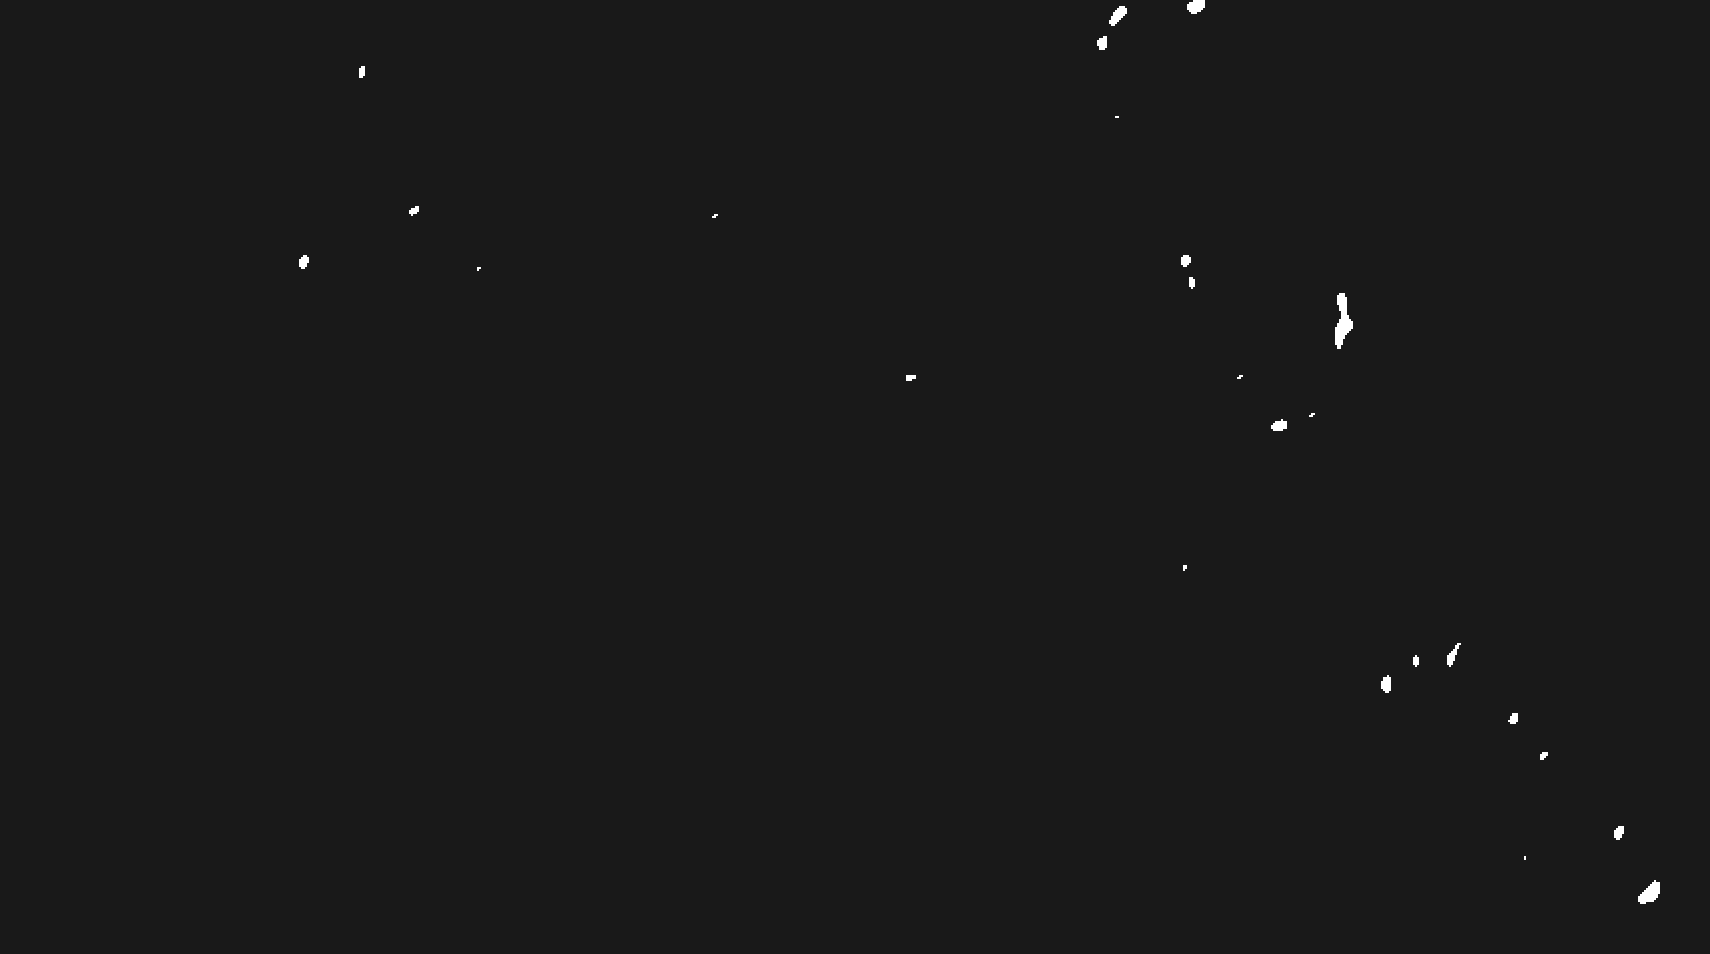
\includegraphics[width=.3\textwidth]{Imagenes/Homomorfico/Paranai1_bin.png}\hfill
    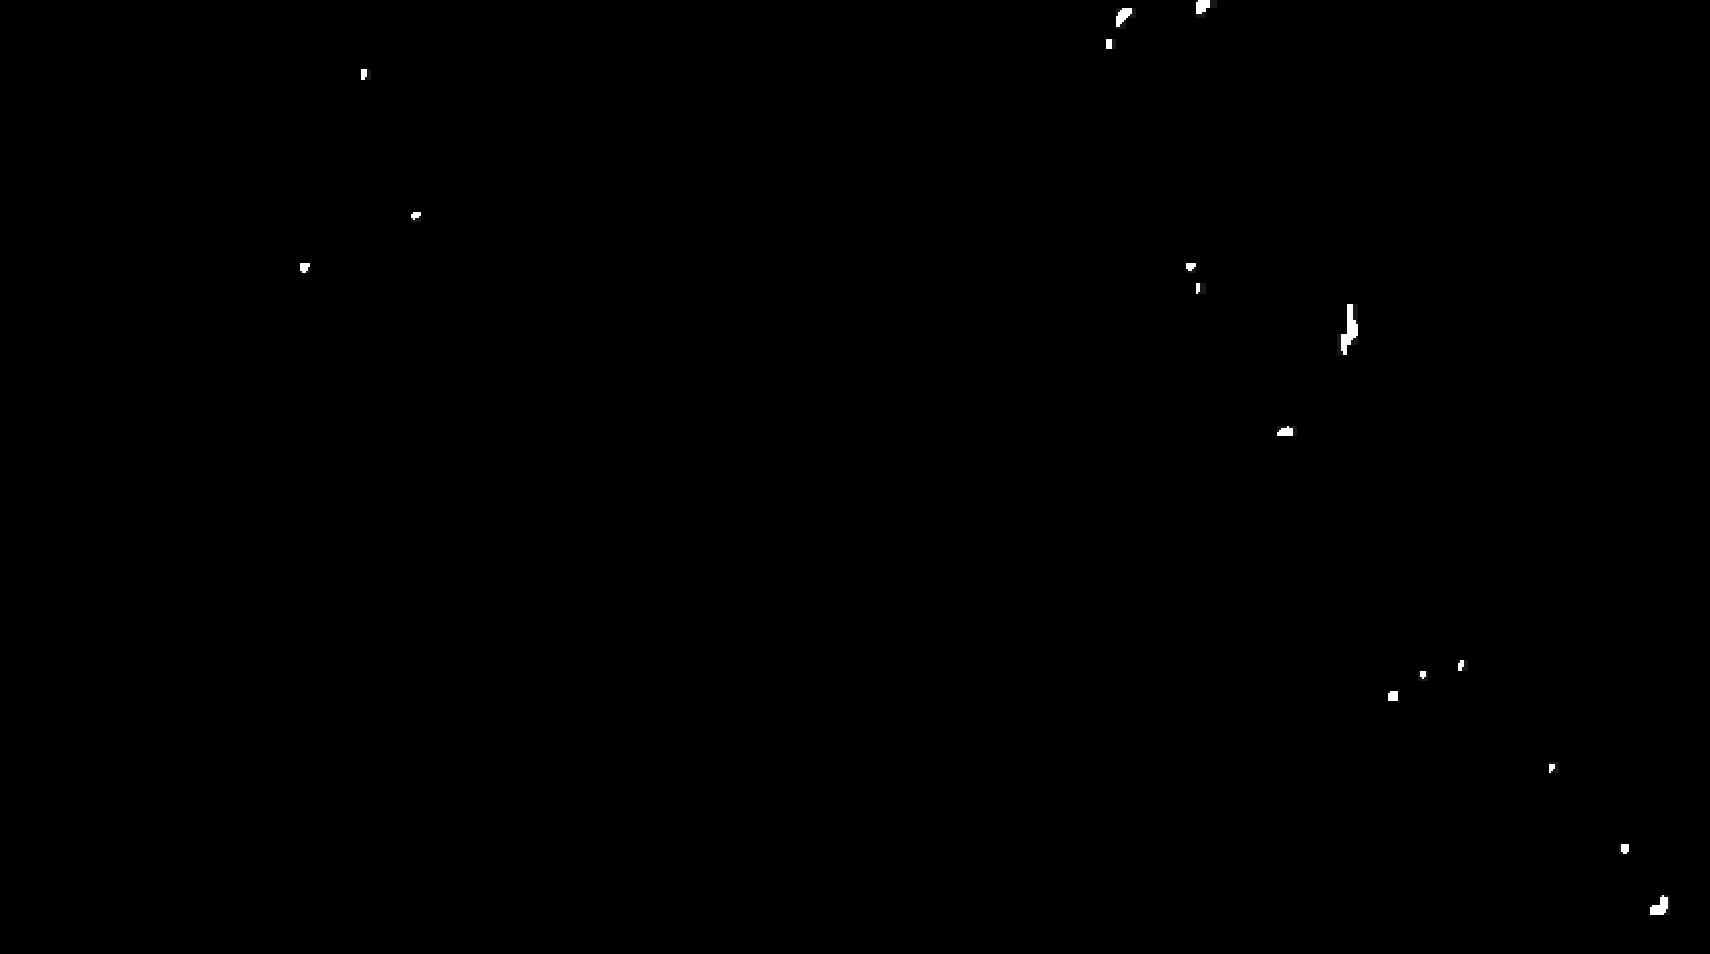
\includegraphics[width=.3\textwidth]{Imagenes/Homomorfico/Paranai1_masked_10.png}\hfill
    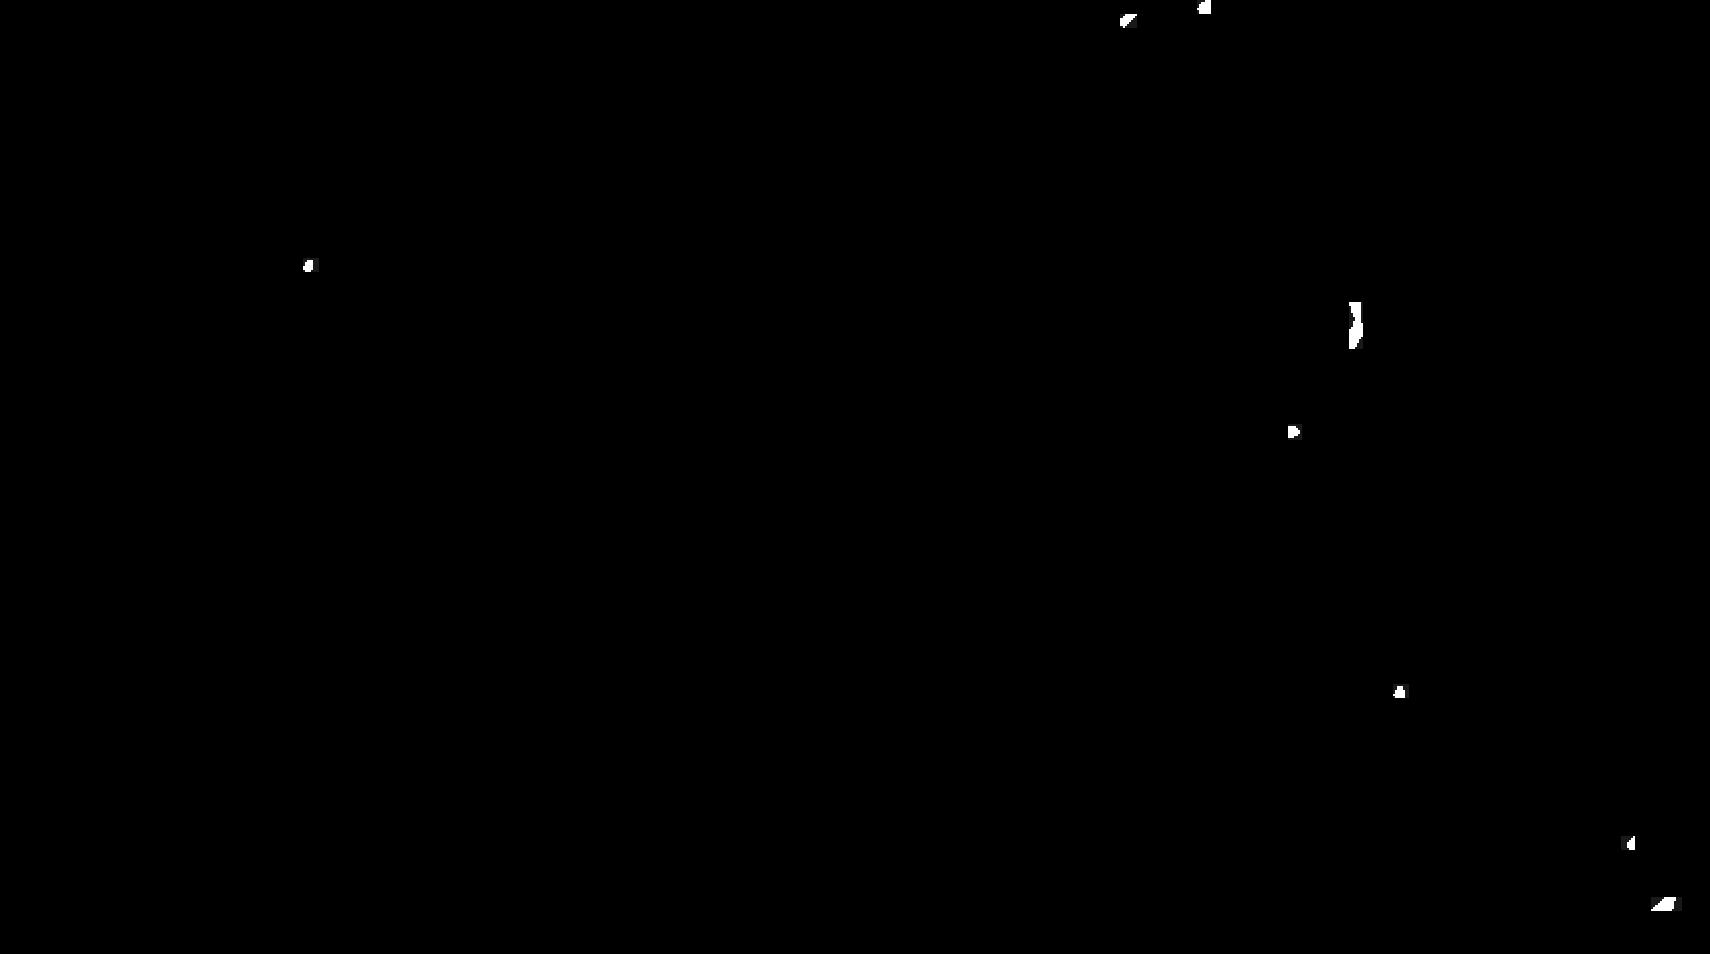
\includegraphics[width=.3\textwidth]{Imagenes/Homomorfico/Paranai1_masked_15.png}\hfill
    \\[\smallskipamount]
    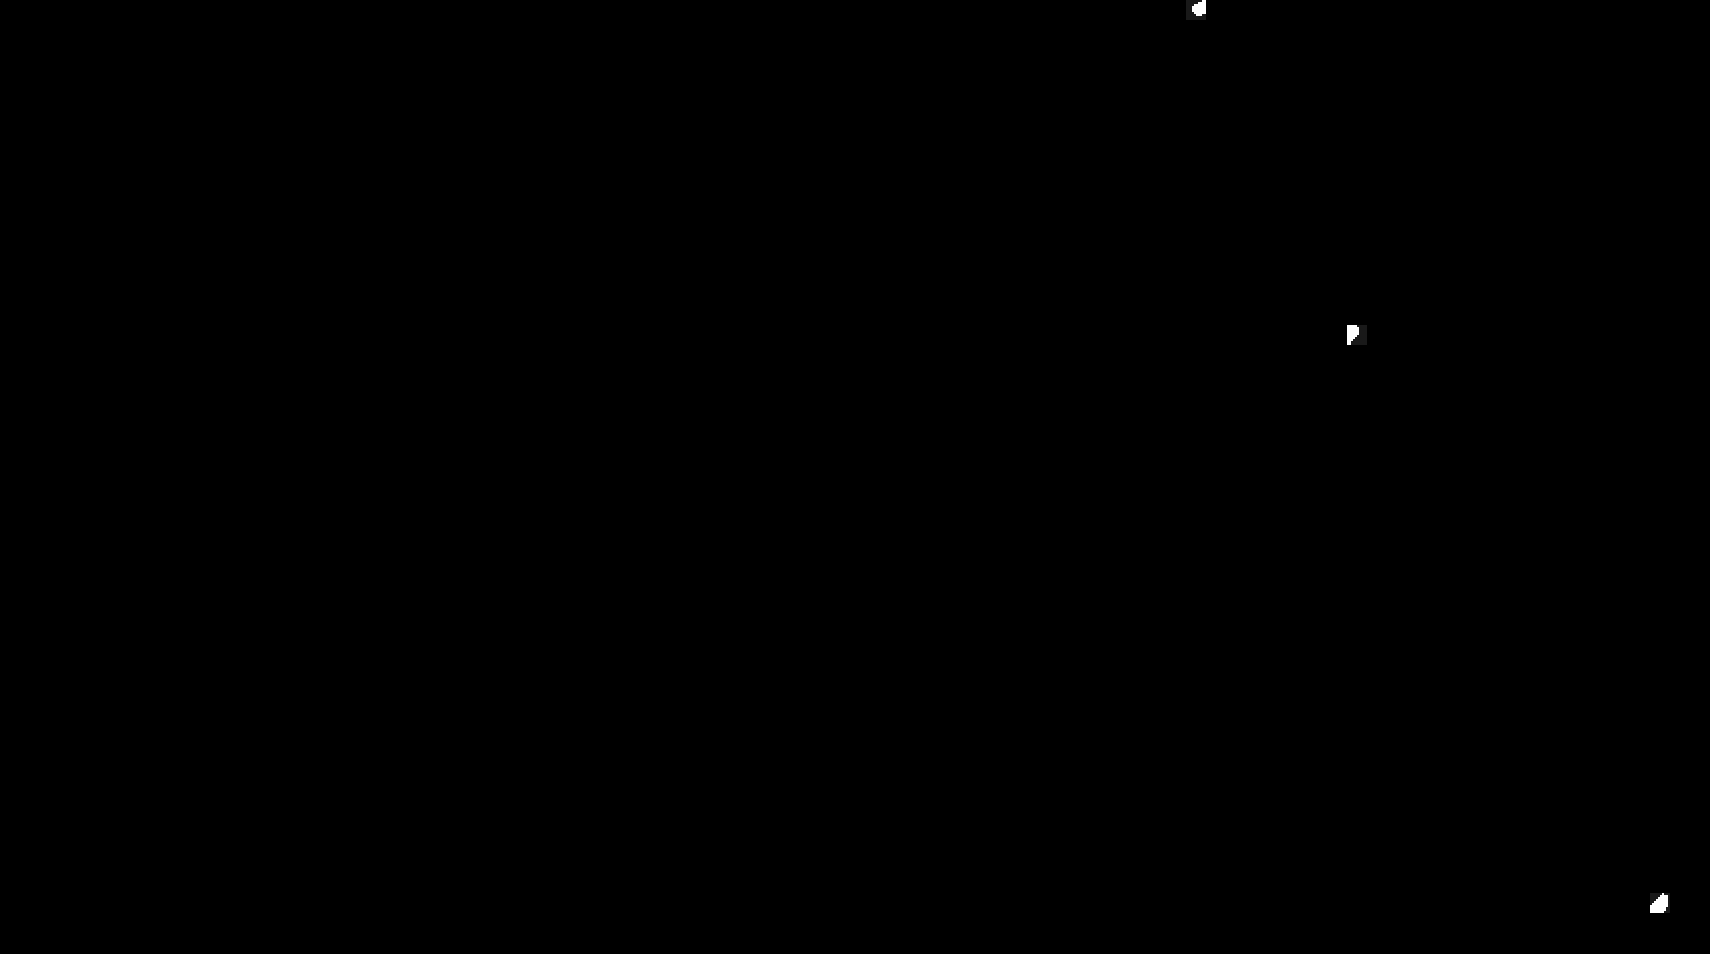
\includegraphics[width=.3\textwidth]{Imagenes/Homomorfico/Paranai1_masked_20.png}\hfill
    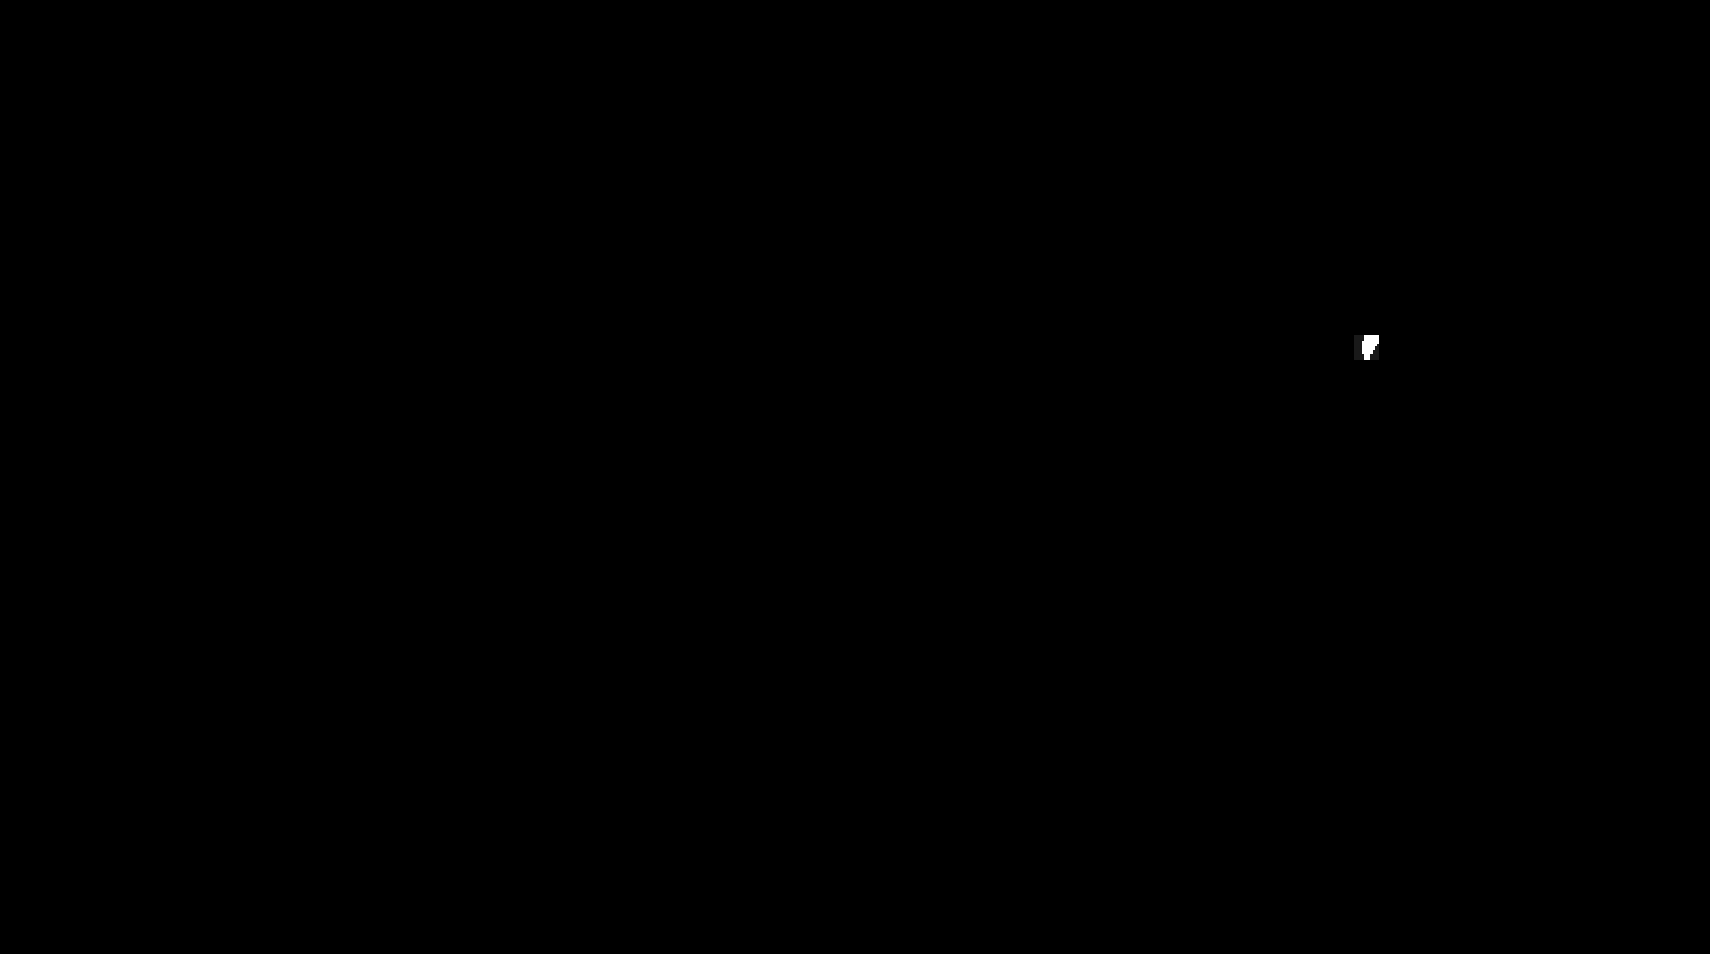
\includegraphics[width=.3\textwidth]{Imagenes/Homomorfico/Paranai1_masked_25.png}\hfill
    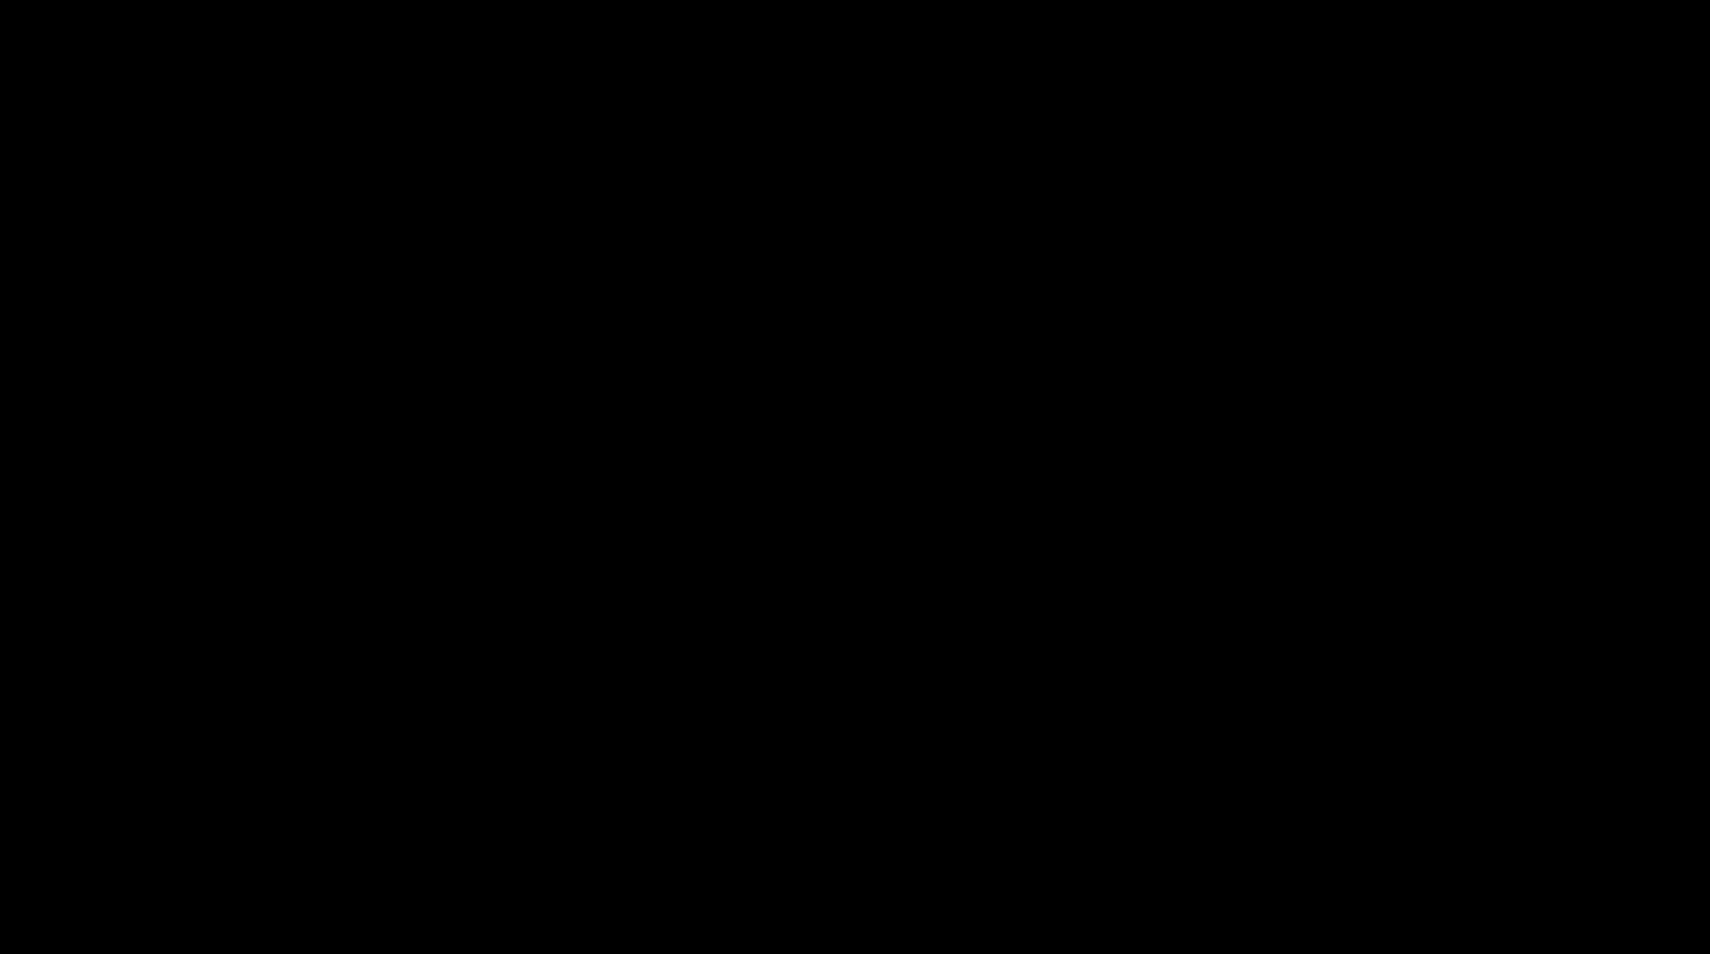
\includegraphics[width=.3\textwidth]{Imagenes/Homomorfico/Paranai1_masked_30.png}\hfill
    
    \caption{Máscara binaria, sombras seleccionadas con ventana de 10, 15, 20, 25 y 30 píxeles}\label{fig:paranai1}
\end{figure}

\begin{figure}[h!]
    \includegraphics[width=0.5\textwidth]{Imagenes/Homomorfico/Paranai2eq.png}
     \hfill
     \caption{Imagen aérea (satelital) de una porción de selva nativa y terrenos cultivados junto al arroyo Paranay}
    %\label{Paranay2}
\end{figure}

\begin{figure}
    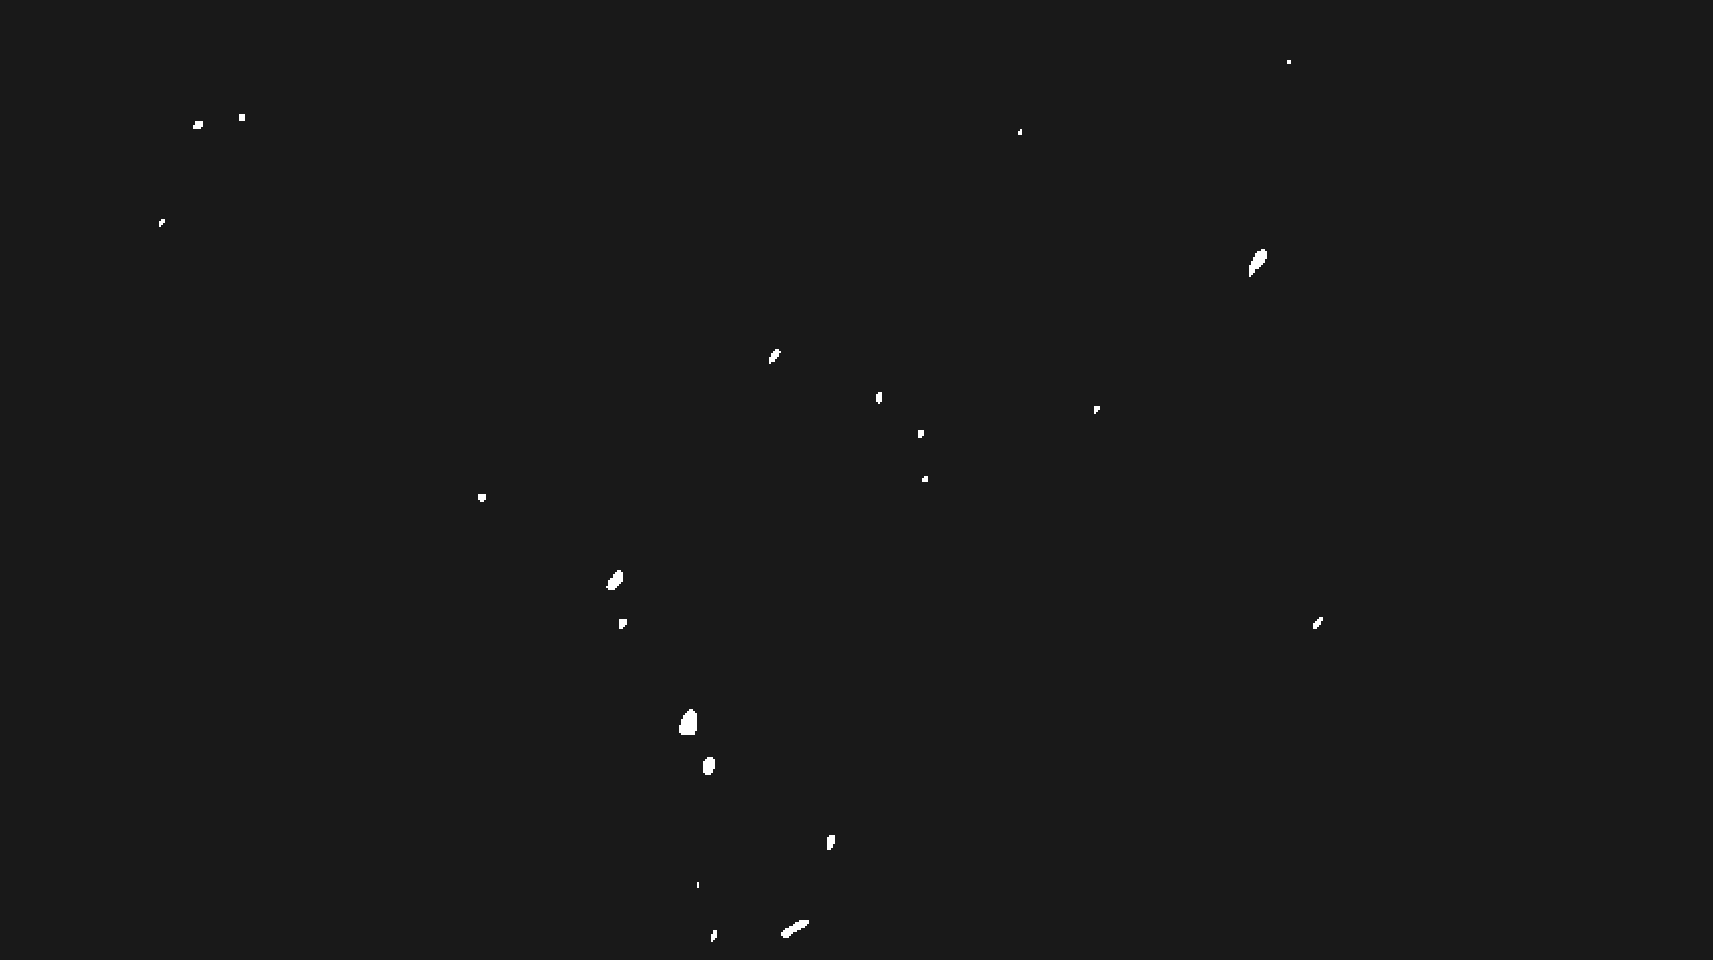
\includegraphics[width=.3\textwidth]{Imagenes/Homomorfico/Paranai2_bin.png}\hfill
    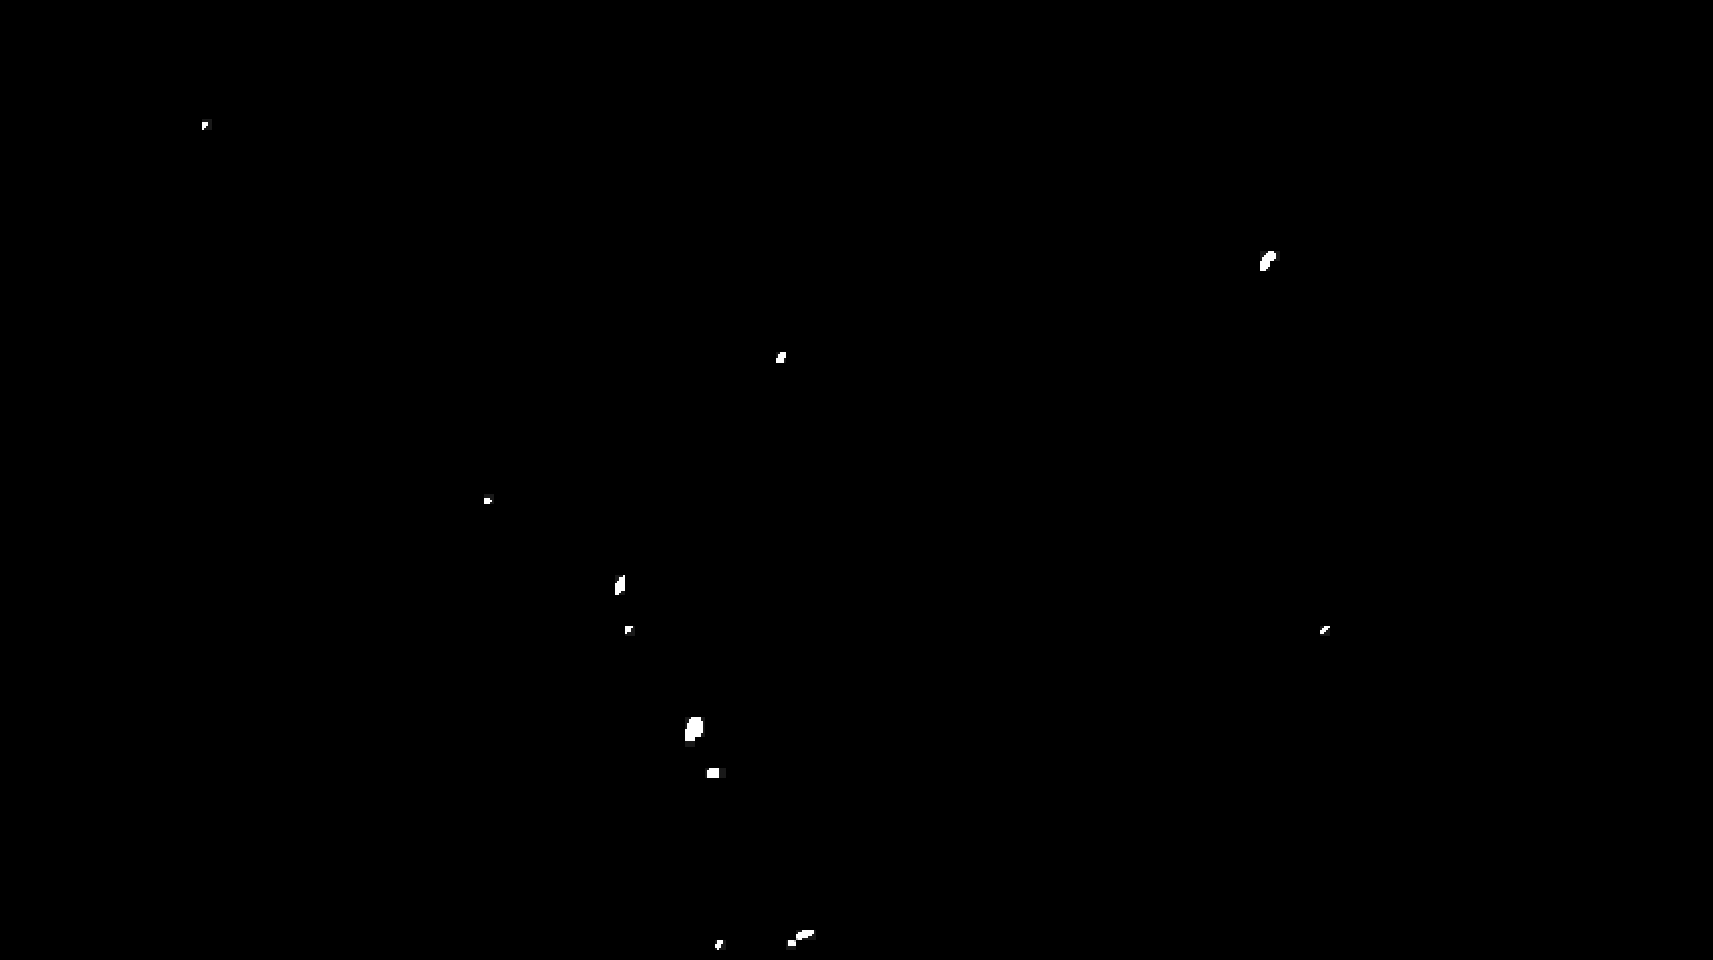
\includegraphics[width=.3\textwidth]{Imagenes/Homomorfico/Paranai2_masked_10.png}\hfill
    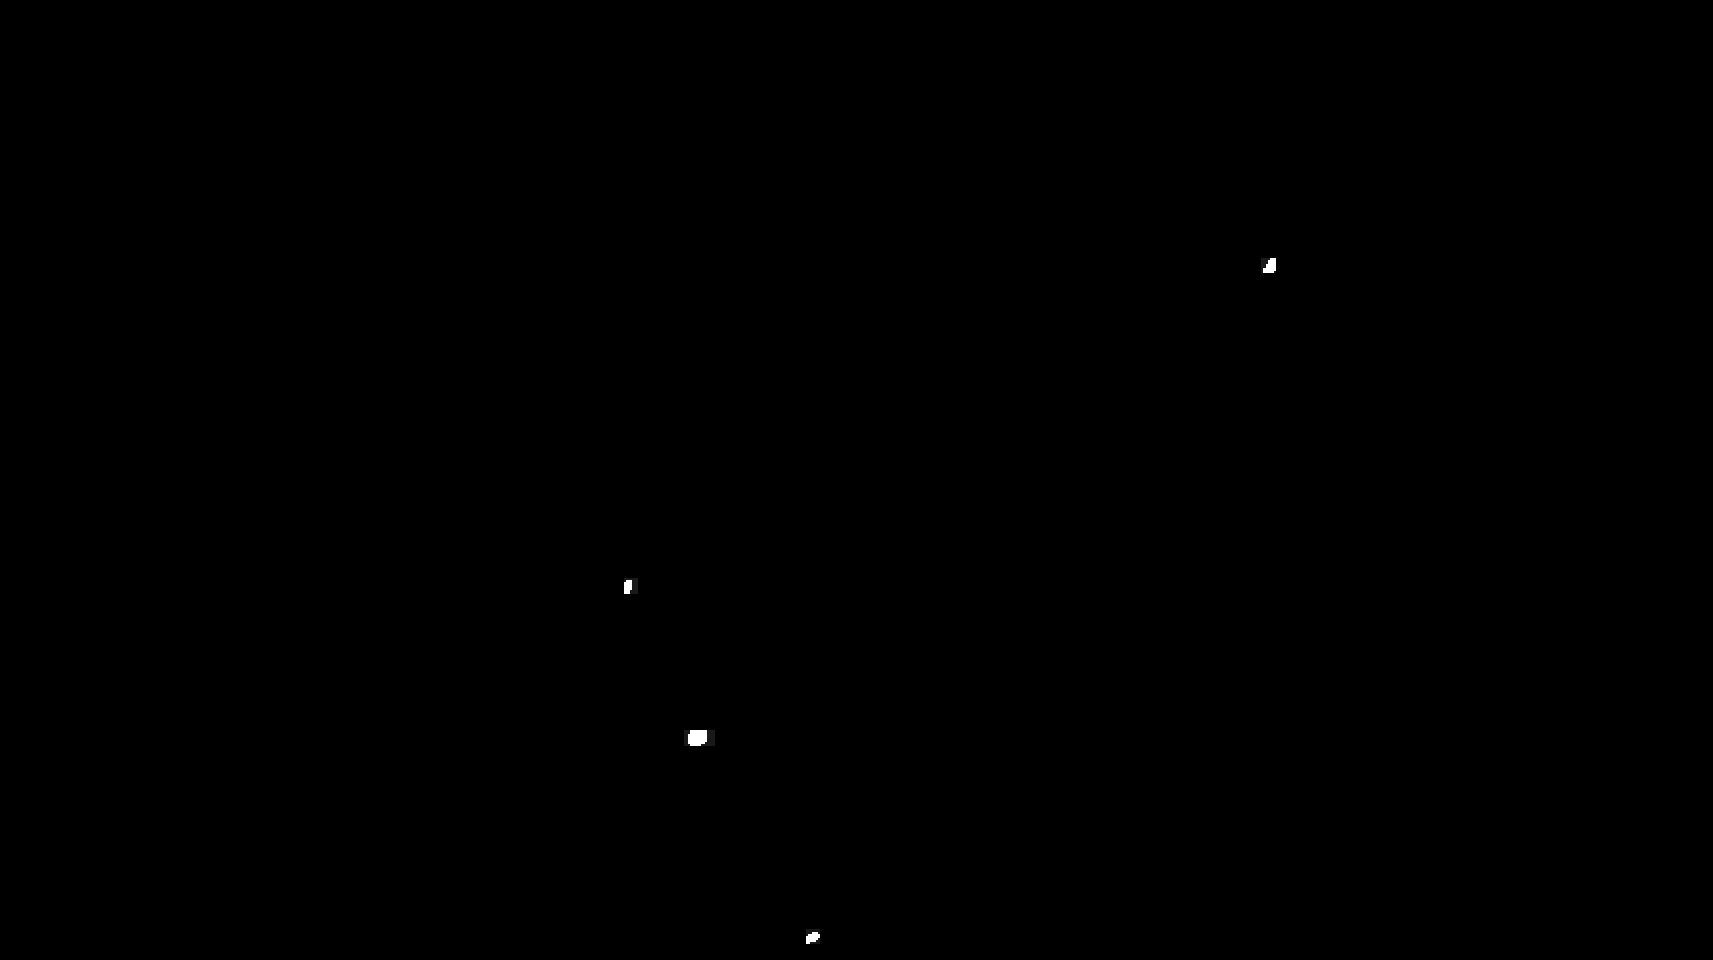
\includegraphics[width=.3\textwidth]{Imagenes/Homomorfico/Paranai2_masked_15.png}\hfill
    \\[\smallskipamount]
    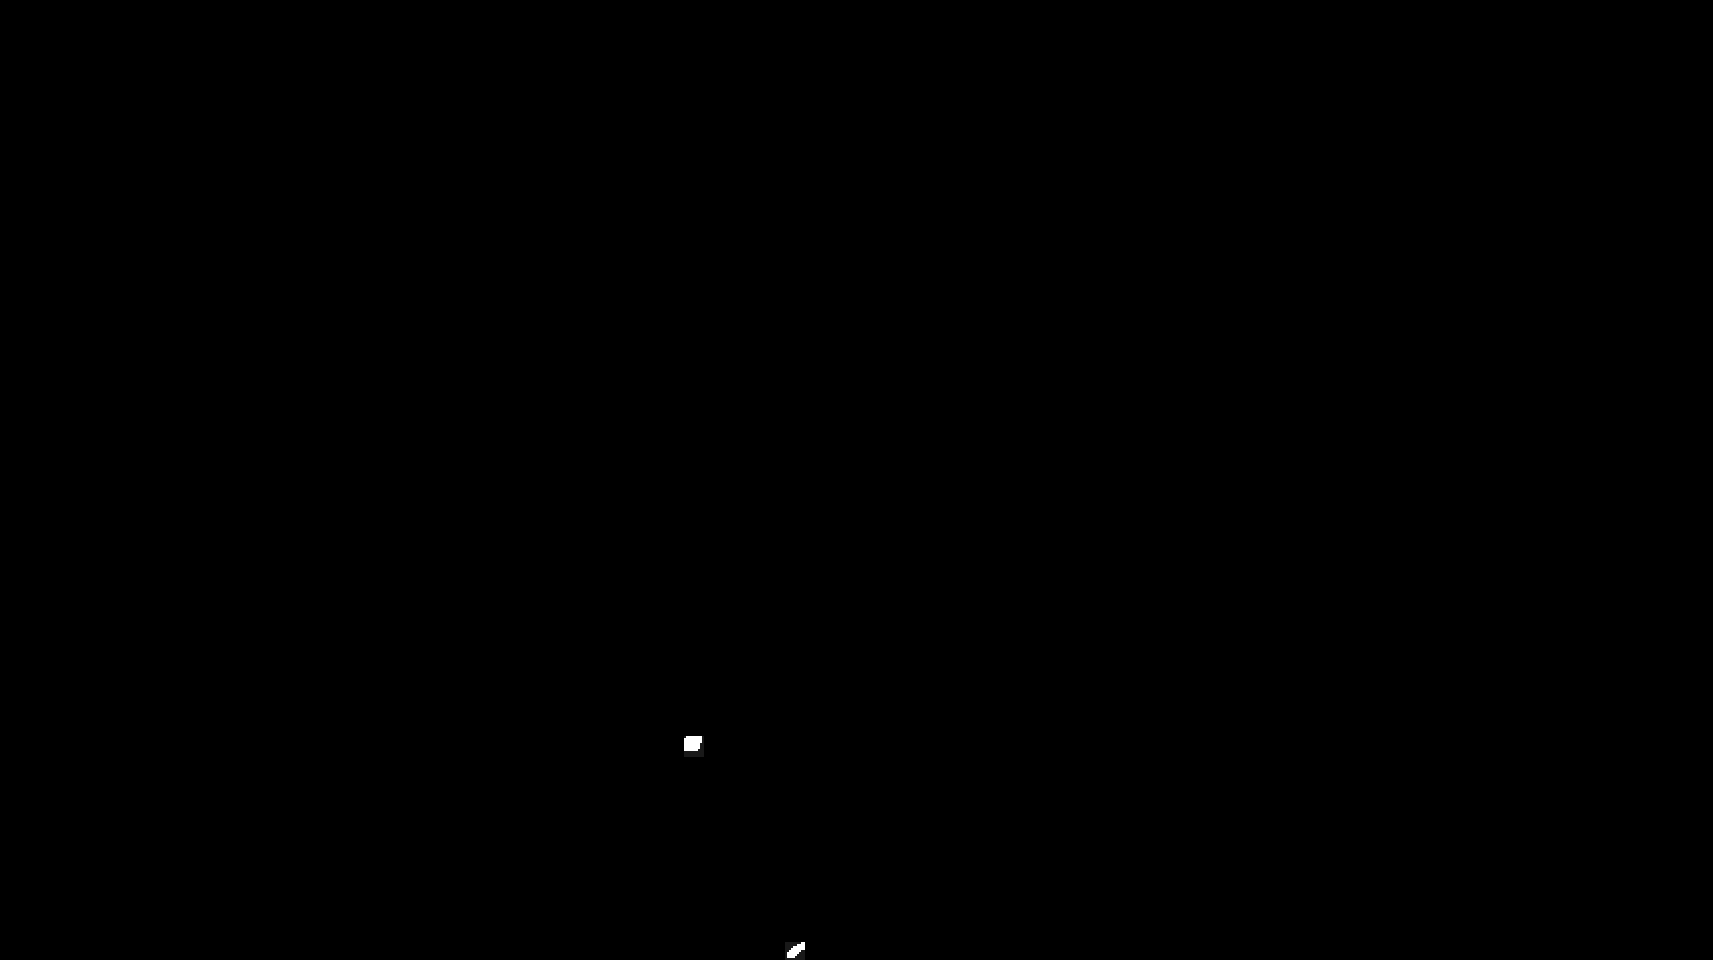
\includegraphics[width=.3\textwidth]{Imagenes/Homomorfico/Paranai2_masked_20.png}\hfill
    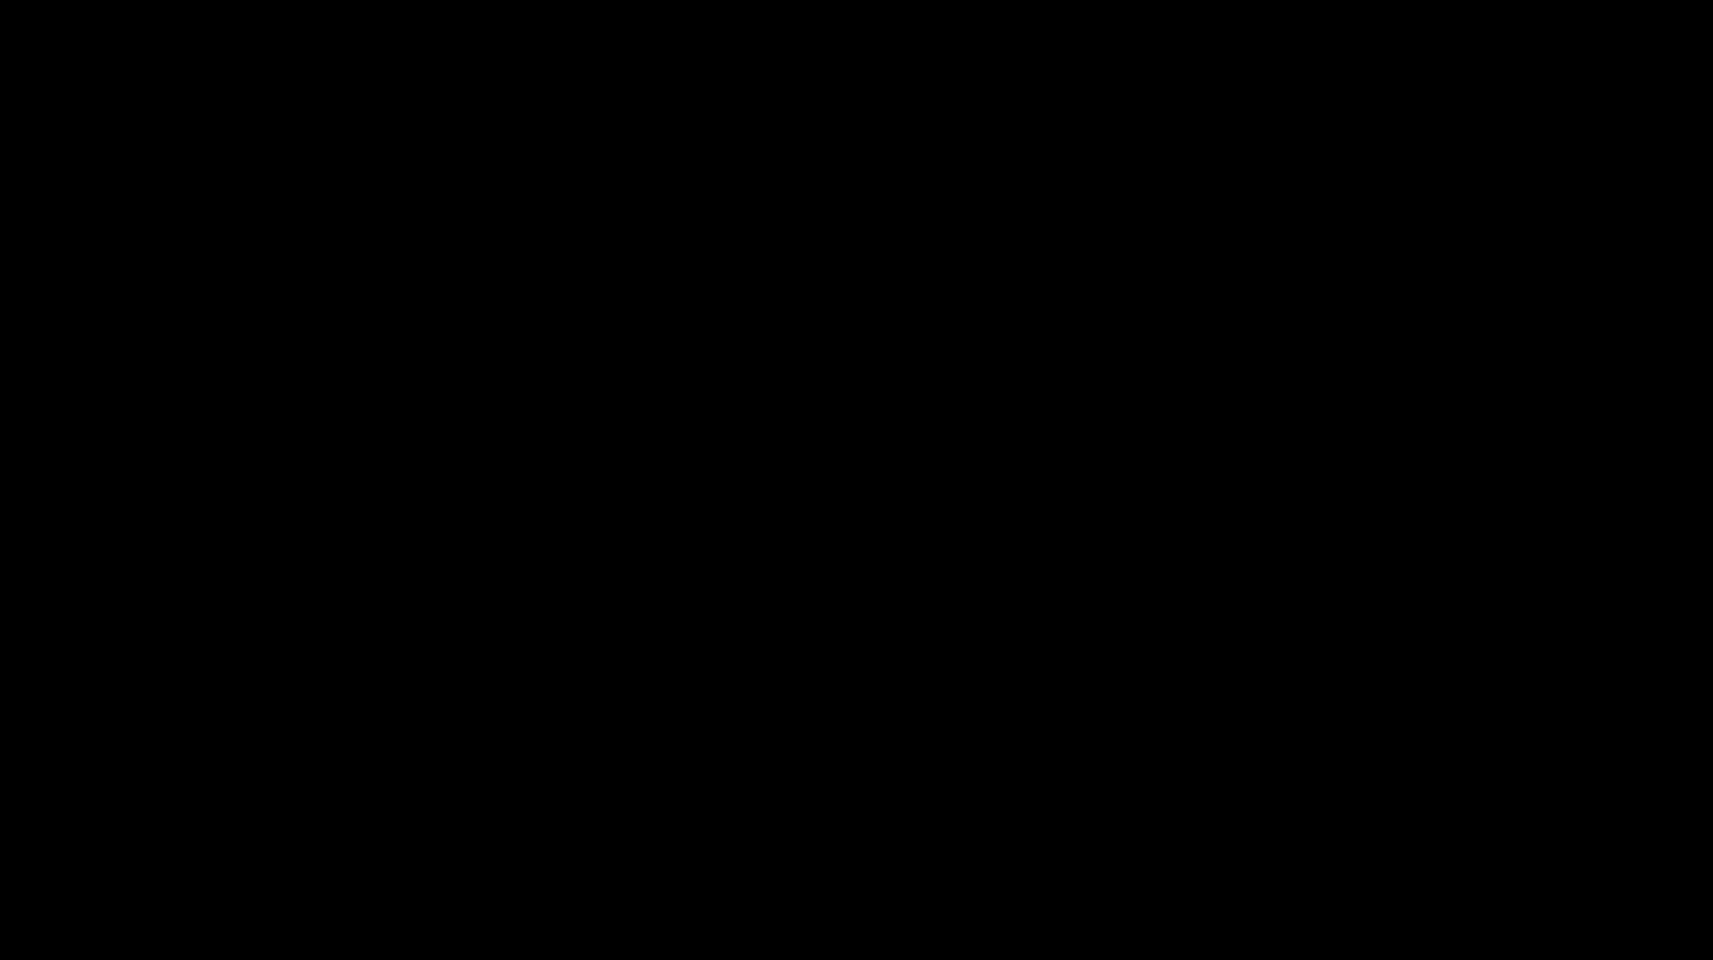
\includegraphics[width=.3\textwidth]{Imagenes/Homomorfico/Paranai2_masked_25.png}\hfill
    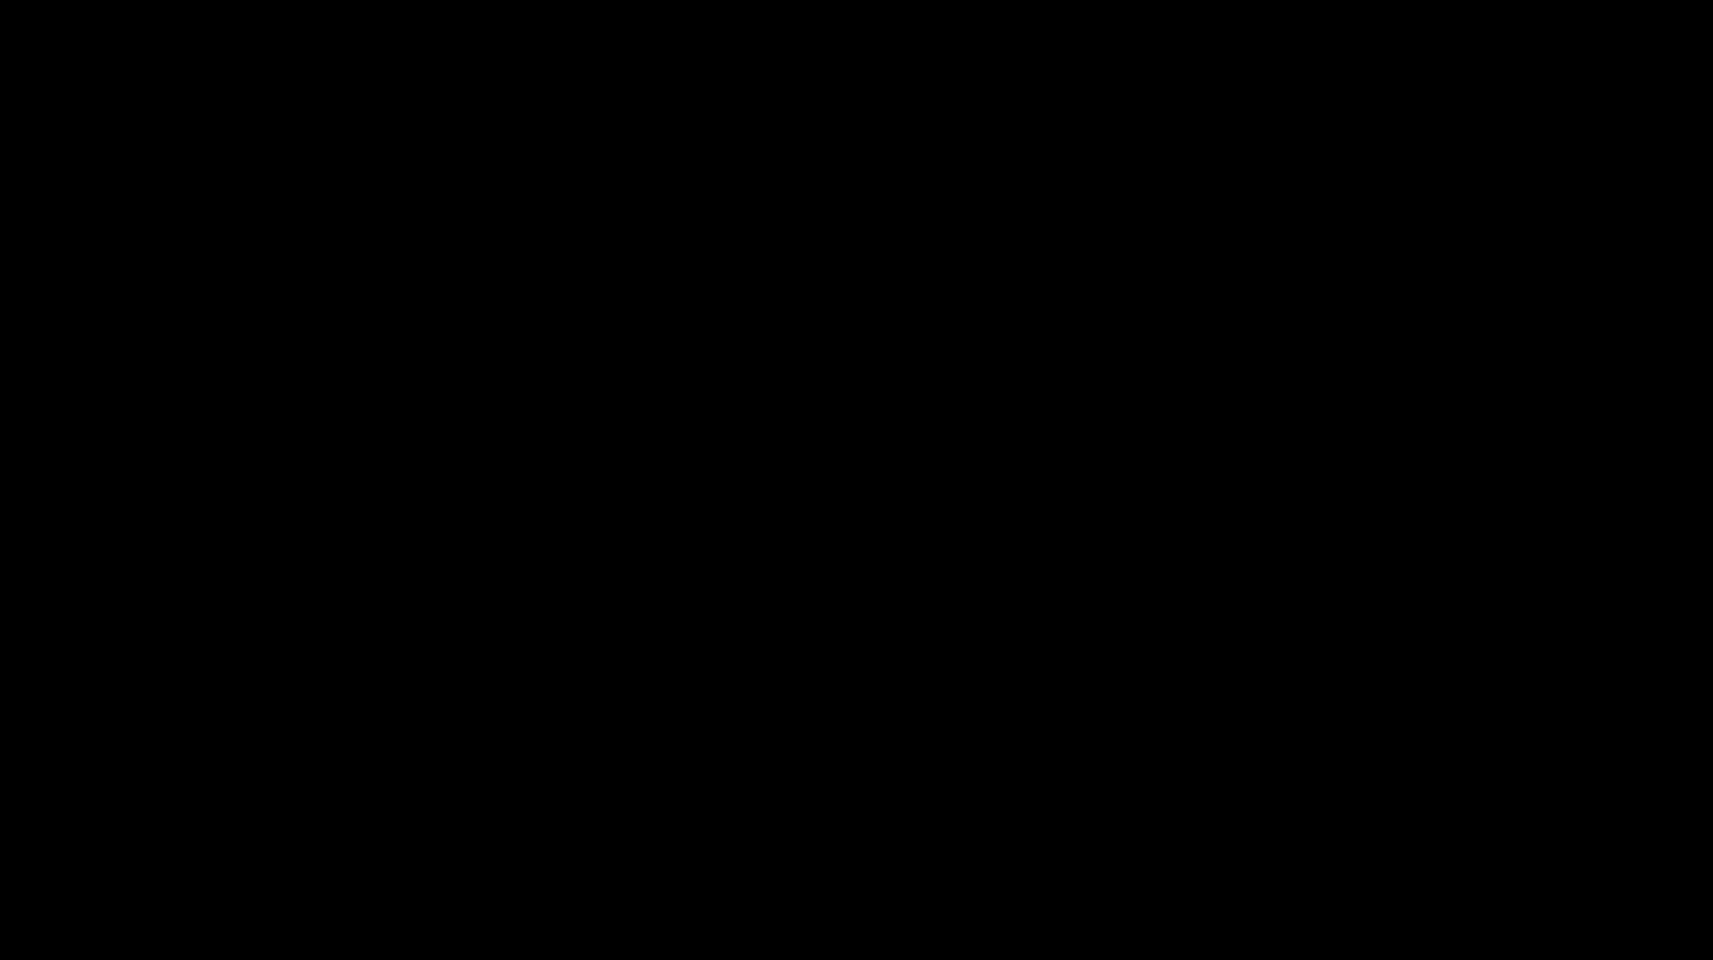
\includegraphics[width=.3\textwidth]{Imagenes/Homomorfico/Paranai2_masked_30.png}\hfill
    
    \caption{Máscara binaria, sombras seleccionadas con ventana de 10, 15, 20, 25 y 30 píxeles}\label{fig:Paranai2}
\end{figure}

\begin{figure}[h!]
    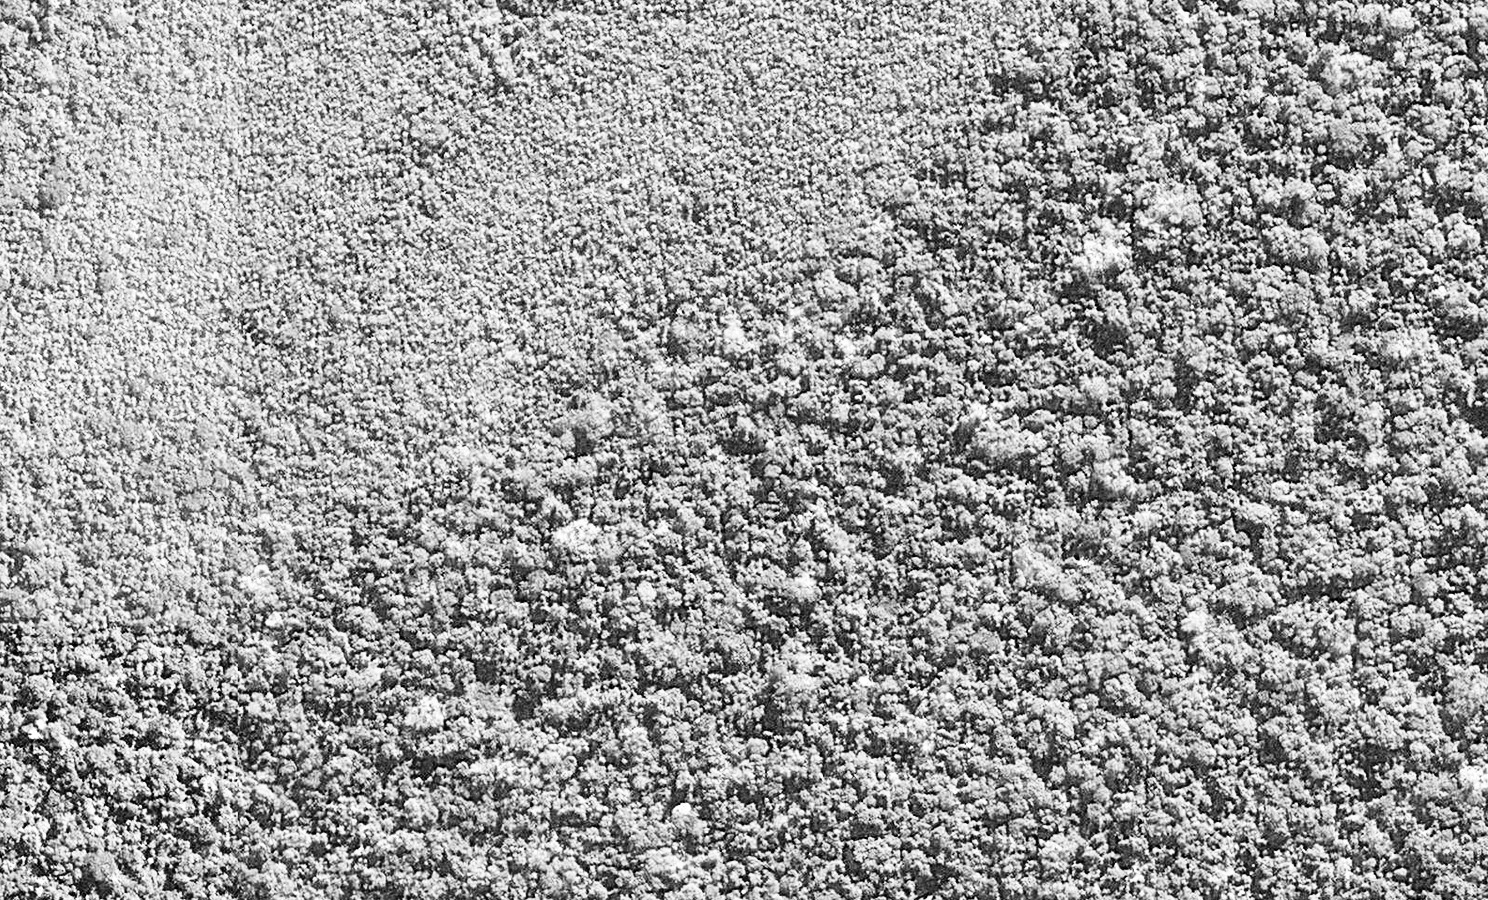
\includegraphics[width=0.5\textwidth]{Imagenes/Homomorfico/PNI1gris.jpg}
     \hfill
     \caption{Imagen aérea (satelital) Parque Nacional Iguazú, en escala de grises}
    %\label{PNI1}
\end{figure}



\begin{figure}[h!]
    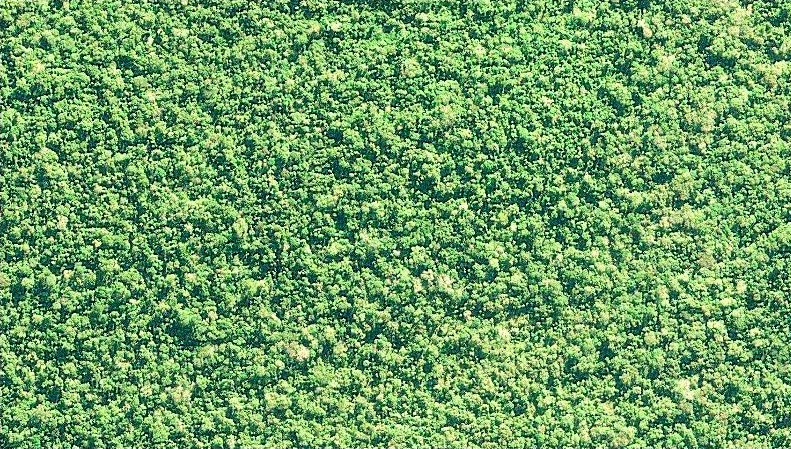
\includegraphics[width=0.5\textwidth]{Imagenes/Homomorfico/PNI2_original.jpg}
     \hfill
     \caption{Imagen aérea (satelital) Parque Nacional Iguazú, en RGB}
    %\label{PNI2}
\end{figure}

\begin{figure}
    
\includegraphics[width=.3\textwidth]{Imagenes/Homomorfico/PNI2_bin.png}\hfill
    
\includegraphics[width=.3\textwidth]{Imagenes/Homomorfico/PNI2_masked_10.png}\hfill
    
\includegraphics[width=.3\textwidth]{Imagenes/Homomorfico/PNI2_masked_15.png}\hfill
    \\[\smallskipamount]
    
\includegraphics[width=.3\textwidth]{Imagenes/Homomorfico/PNI2_masked_20.png}\hfill
    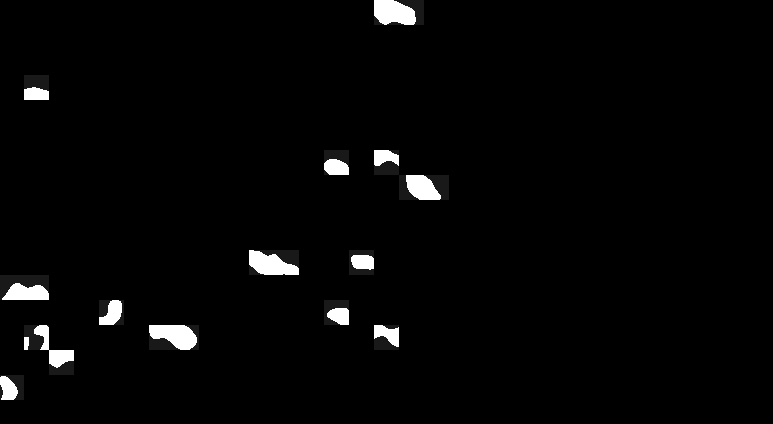
\includegraphics[width=.3\textwidth]{Imagenes/Homomorfico/PNI2_masked_25.png}\hfill
    
\includegraphics[width=.3\textwidth]{Imagenes/Homomorfico/PNI2_masked_30.png}\hfill
    
    \caption{Máscara binaria, sombras seleccionadas con ventana de 10, 15, 20, 25 y 30 píxeles}\label{fig:Iguazu2}
\end{figure}

\begin{figure}[h!]
    \includegraphics[width=0.5\textwidth]{Imagenes/Homomorfico/PNI_03.jpg}
     \hfill
     \caption{Imagen aérea (satelital) Parque Nacional Iguazú, en RGB}
    %  \label{PNI3}
\end{figure}


\begin{figure}[h!]
    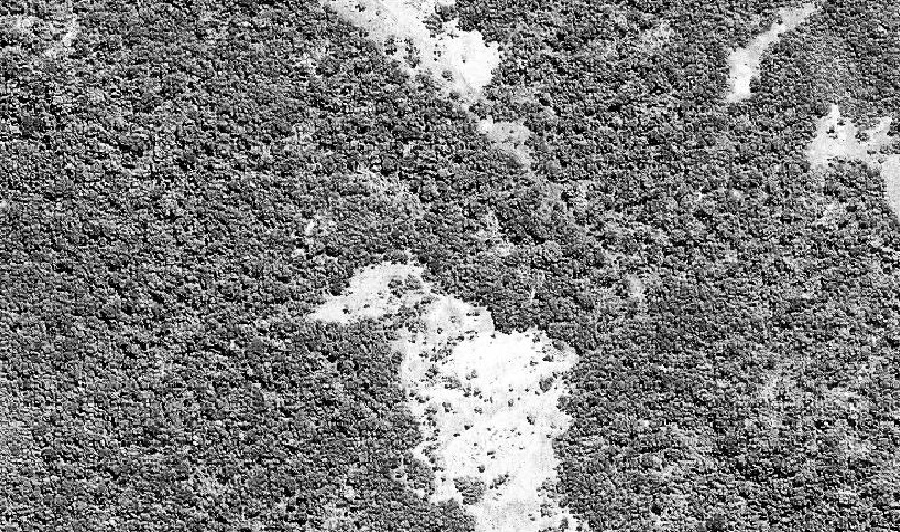
\includegraphics[width=0.5\textwidth]{Imagenes/Homomorfico/PS1_original.jpg}
     \hfill
     \caption{Imagen aérea (satelital) Parque de la Sierra, en RGB}
    %  \label{PS1}
\end{figure}

\begin{figure}
    
\includegraphics[width=.3\textwidth]{Imagenes/Homomorfico/PS1_bin.png}\hfill
    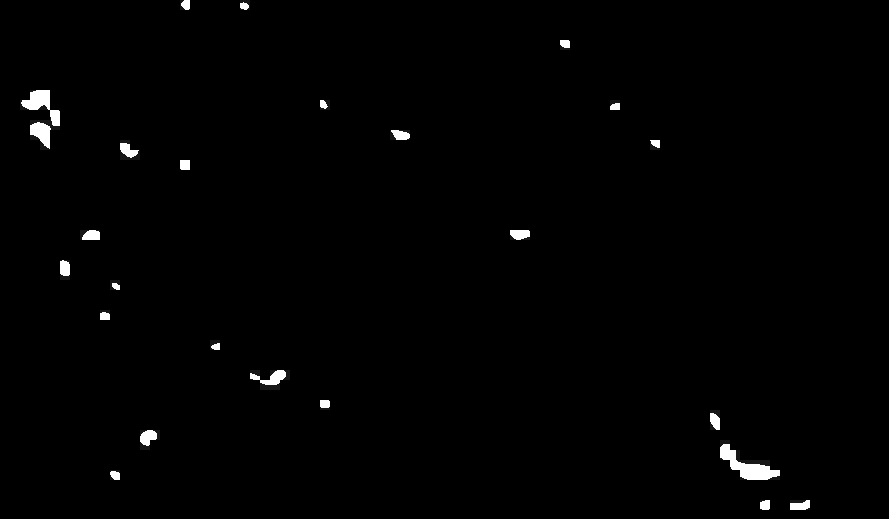
\includegraphics[width=.3\textwidth]{Imagenes/Homomorfico/PS1_masked_10.png}\hfill
    \includegraphics[width=.3\textwidth]{Imagenes/Homomorfico/PS1_masked_15.png}\hfill
    \\[\smallskipamount]
    \includegraphics[width=.3\textwidth]{Imagenes/Homomorfico/PS1_masked_20.png}\hfill
    \includegraphics[width=.3\textwidth]{Imagenes/Homomorfico/PS1_masked_25.png}\hfill
    \includegraphics[width=.3\textwidth]{Imagenes/Homomorfico/PS1_masked_30.png}\hfill
    
    \caption{Máscara binaria, sombras seleccionadas con ventana de 10, 15, 20, 25 y 30 píxeles}\label{fig:Parque de la Sierra 1}
\end{figure}

\begin{figure}[h!]
    \includegraphics[width=0.5\textwidth]{Imagenes/Homomorfico/YB1.jpg}
     \hfill
     \caption{Imagen aérea (satelital) Biósfera Yaboty, en RGB}
    %  \label{YB1}
\end{figure}

\begin{figure}
    \includegraphics[width=.3\textwidth]{Imagenes/Homomorfico/YB1_bin.png}\hfill
    \includegraphics[width=.3\textwidth]{Imagenes/Homomorfico/YB1_masked_10.png}\hfill
    \includegraphics[width=.3\textwidth]{Imagenes/Homomorfico/YB1_masked_15.png}\hfill
    \\[\smallskipamount]
    \includegraphics[width=.3\textwidth]{Imagenes/Homomorfico/YB1_masked_20.png}\hfill
    \includegraphics[width=.3\textwidth]{Imagenes/Homomorfico/YB1_masked_25.png}\hfill
    \includegraphics[width=.3\textwidth]{Imagenes/Homomorfico/YB1_masked_30.png}\hfill
    
    \caption{Máscara binaria, sombras seleccionadas con ventana de 10, 15, 20, 25 y 30 píxeles}\label{fig:Yaboty1}
\end{figure}

\begin{figure}[h!]
    \includegraphics[width=0.5\textwidth]{Imagenes/Homomorfico/YB2.jpg}
     \hfill
     \caption{Imagen aérea (satelital) Biósfera Yaboty, en RGB}
    %  \label{YB2}
\end{figure}

\begin{figure}
    \includegraphics[width=.3\textwidth]{Imagenes/Homomorfico/YB2_bin.png}\hfill
    \includegraphics[width=.3\textwidth]{Imagenes/Homomorfico/YB2_masked_10.png}\hfill
    \includegraphics[width=.3\textwidth]{Imagenes/Homomorfico/YB2_masked_15.png}\hfill
    \\[\smallskipamount]
    \includegraphics[width=.3\textwidth]{Imagenes/Homomorfico/YB2_masked_20.png}\hfill
    \includegraphics[width=.3\textwidth]{Imagenes/Homomorfico/YB2_masked_25.png}\hfill
    \includegraphics[width=.3\textwidth]{Imagenes/Homomorfico/YB2_masked_30.png}\hfill
    
    \caption{Máscara binaria, sombras seleccionadas con ventana de 10, 15, 20, 25 y 30 píxeles}\label{fig:Yaboty2}
\end{figure}

\begin{figure}[h!]
    \includegraphics[width=0.5\textwidth]{Imagenes/Homomorfico/ST1_gris.png}
     \hfill
     \caption{Imagen aérea (satelital) reserva privada Sombra de Toro, en escala de grises}
    %  \label{ST1}
\end{figure}

\begin{figure}
    \includegraphics[width=.3\textwidth]{Imagenes/Homomorfico/ST1_bin.png}\hfill
    \includegraphics[width=.3\textwidth]{Imagenes/Homomorfico/ST1_masked_10.png}\hfill
    \includegraphics[width=.3\textwidth]{Imagenes/Homomorfico/ST1_masked_15.png}\hfill
    \\[\smallskipamount]
    \includegraphics[width=.3\textwidth]{Imagenes/Homomorfico/ST1_masked_20.png}\hfill
    \includegraphics[width=.3\textwidth]{Imagenes/Homomorfico/ST1_masked_25.png}\hfill
    \includegraphics[width=.3\textwidth]{Imagenes/Homomorfico/ST1_masked_30.png}\hfill
    
    \caption{Máscara binaria, sombras seleccionadas con ventana de 10, 15, 20, 25 y 30 píxeles}\label{fig:Storo1}
\end{figure}

\begin{figure}[h!]
    \includegraphics[width=0.5\textwidth]{Imagenes/Homomorfico/ST2.png}
     \hfill
     \caption{Imagen aérea (satelital) reserva privada Sombra de Toro, en RGB}
    %  \label{ST2}
\end{figure}

\begin{figure}
    \includegraphics[width=.3\textwidth]{Imagenes/Homomorfico/ST2_bin.png}\hfill
    \includegraphics[width=.3\textwidth]{Imagenes/Homomorfico/ST2_masked_10.png}\hfill
    \includegraphics[width=.3\textwidth]{Imagenes/Homomorfico/ST2_masked_15.png}\hfill
    \\[\smallskipamount]
    \includegraphics[width=.3\textwidth]{Imagenes/Homomorfico/ST2_masked_20.png}\hfill
    \includegraphics[width=.3\textwidth]{Imagenes/Homomorfico/ST2_masked_25.png}\hfill
    \includegraphics[width=.3\textwidth]{Imagenes/Homomorfico/ST2_masked_30.png}\hfill
    
    \caption{Máscara binaria, sombras seleccionadas con ventana de 10, 15, 20, 25 y 30 píxeles}\label{fig:Storo2}
\end{figure}


\chapter{Imágenes procesadas por método morfológico} \label{anexo_morfo}
  %%Anexo con imágenes analizadas con algoritmo de procesamiento homomórfico

\begin{figure}[h!]
    \includegraphics[width=0.5\textwidth]{Imagenes/Homomorfico/Paranai1eq.png}
     \hfill
     \caption{Imagen aérea (satelital) de una porción de selva nativa y terrenos cultivados junto al arroyo Paranay }
    %\label{Paranay1}
\end{figure}

\begin{figure}
    \includegraphics[width=.3\textwidth]{Imagenes/Homomorfico/Paranai1_bin.png}\hfill
    \includegraphics[width=.3\textwidth]{Imagenes/Homomorfico/Paranai1_masked_10.png}\hfill
    \includegraphics[width=.3\textwidth]{Imagenes/Homomorfico/Paranai1_masked_15.png}\hfill
    \\[\smallskipamount]
    \includegraphics[width=.3\textwidth]{Imagenes/Homomorfico/Paranai1_masked_20.png}\hfill
    \includegraphics[width=.3\textwidth]{Imagenes/Homomorfico/Paranai1_masked_25.png}\hfill
    \includegraphics[width=.3\textwidth]{Imagenes/Homomorfico/Paranai1_masked_30.png}\hfill
    
    \caption{Máscara binaria, sombras seleccionadas con ventana de 10, 15, 20, 25 y 30 píxeles}\label{fig:paranai1}
\end{figure}

\begin{figure}[h!]
    \includegraphics[width=0.5\textwidth]{Imagenes/Homomorfico/Paranai2eq.png}
     \hfill
     \caption{Imagen aérea (satelital) de una porción de selva nativa y terrenos cultivados junto al arroyo Paranay}
    %\label{Paranay2}
\end{figure}

\begin{figure}
    \includegraphics[width=.3\textwidth]{Imagenes/Homomorfico/Paranai2_bin.png}\hfill
    \includegraphics[width=.3\textwidth]{Imagenes/Homomorfico/Paranai2_masked_10.png}\hfill
    \includegraphics[width=.3\textwidth]{Imagenes/Homomorfico/Paranai2_masked_15.png}\hfill
    \\[\smallskipamount]
    \includegraphics[width=.3\textwidth]{Imagenes/Homomorfico/Paranai2_masked_20.png}\hfill
    \includegraphics[width=.3\textwidth]{Imagenes/Homomorfico/Paranai2_masked_25.png}\hfill
    \includegraphics[width=.3\textwidth]{Imagenes/Homomorfico/Paranai2_masked_30.png}\hfill
    
    \caption{Máscara binaria, sombras seleccionadas con ventana de 10, 15, 20, 25 y 30 píxeles}\label{fig:Paranai2}
\end{figure}

\begin{figure}[h!]
    \includegraphics[width=0.5\textwidth]{Imagenes/Homomorfico/PNI1gris.jpg}
     \hfill
     \caption{Imagen aérea (satelital) Parque Nacional Iguazú, en escala de grises}
    %\label{PNI1}
\end{figure}



\begin{figure}[h!]
    \includegraphics[width=0.5\textwidth]{Imagenes/Homomorfico/PNI2_original.jpg}
     \hfill
     \caption{Imagen aérea (satelital) Parque Nacional Iguazú, en RGB}
    %\label{PNI2}
\end{figure}

\begin{figure}
    \includegraphics[width=.3\textwidth]{Imagenes/Homomorfico/PNI2_bin.png}\hfill
    \includegraphics[width=.3\textwidth]{Imagenes/Homomorfico/PNI2_masked_10.png}\hfill
    \includegraphics[width=.3\textwidth]{Imagenes/Homomorfico/PNI2_masked_15.png}\hfill
    \\[\smallskipamount]
    \includegraphics[width=.3\textwidth]{Imagenes/Homomorfico/PNI2_masked_20.png}\hfill
    \includegraphics[width=.3\textwidth]{Imagenes/Homomorfico/PNI2_masked_25.png}\hfill
    \includegraphics[width=.3\textwidth]{Imagenes/Homomorfico/PNI2_masked_30.png}\hfill
    
    \caption{Máscara binaria, sombras seleccionadas con ventana de 10, 15, 20, 25 y 30 píxeles}\label{fig:Iguazu2}
\end{figure}

\begin{figure}[h!]
    \includegraphics[width=0.5\textwidth]{Imagenes/Homomorfico/PNI_03.jpg}
     \hfill
     \caption{Imagen aérea (satelital) Parque Nacional Iguazú, en RGB}
    %  \label{PNI3}
\end{figure}


\begin{figure}[h!]
    \includegraphics[width=0.5\textwidth]{Imagenes/Homomorfico/PS1_original.jpg}
     \hfill
     \caption{Imagen aérea (satelital) Parque de la Sierra, en RGB}
    %  \label{PS1}
\end{figure}

\begin{figure}
    \includegraphics[width=.3\textwidth]{Imagenes/Homomorfico/PS1_bin.png}\hfill
    \includegraphics[width=.3\textwidth]{Imagenes/Homomorfico/PS1_masked_10.png}\hfill
    \includegraphics[width=.3\textwidth]{Imagenes/Homomorfico/PS1_masked_15.png}\hfill
    \\[\smallskipamount]
    \includegraphics[width=.3\textwidth]{Imagenes/Homomorfico/PS1_masked_20.png}\hfill
    \includegraphics[width=.3\textwidth]{Imagenes/Homomorfico/PS1_masked_25.png}\hfill
    \includegraphics[width=.3\textwidth]{Imagenes/Homomorfico/PS1_masked_30.png}\hfill
    
    \caption{Máscara binaria, sombras seleccionadas con ventana de 10, 15, 20, 25 y 30 píxeles}\label{fig:Parque de la Sierra 1}
\end{figure}

\begin{figure}[h!]
    \includegraphics[width=0.5\textwidth]{Imagenes/Homomorfico/YB1.jpg}
     \hfill
     \caption{Imagen aérea (satelital) Biósfera Yaboty, en RGB}
    %  \label{YB1}
\end{figure}

\begin{figure}
    \includegraphics[width=.3\textwidth]{Imagenes/Homomorfico/YB1_bin.png}\hfill
    \includegraphics[width=.3\textwidth]{Imagenes/Homomorfico/YB1_masked_10.png}\hfill
    \includegraphics[width=.3\textwidth]{Imagenes/Homomorfico/YB1_masked_15.png}\hfill
    \\[\smallskipamount]
    \includegraphics[width=.3\textwidth]{Imagenes/Homomorfico/YB1_masked_20.png}\hfill
    \includegraphics[width=.3\textwidth]{Imagenes/Homomorfico/YB1_masked_25.png}\hfill
    \includegraphics[width=.3\textwidth]{Imagenes/Homomorfico/YB1_masked_30.png}\hfill
    
    \caption{Máscara binaria, sombras seleccionadas con ventana de 10, 15, 20, 25 y 30 píxeles}\label{fig:Yaboty1}
\end{figure}

\begin{figure}[h!]
    \includegraphics[width=0.5\textwidth]{Imagenes/Homomorfico/YB2.jpg}
     \hfill
     \caption{Imagen aérea (satelital) Biósfera Yaboty, en RGB}
    %  \label{YB2}
\end{figure}

\begin{figure}
    \includegraphics[width=.3\textwidth]{Imagenes/Homomorfico/YB2_bin.png}\hfill
    \includegraphics[width=.3\textwidth]{Imagenes/Homomorfico/YB2_masked_10.png}\hfill
    \includegraphics[width=.3\textwidth]{Imagenes/Homomorfico/YB2_masked_15.png}\hfill
    \\[\smallskipamount]
    \includegraphics[width=.3\textwidth]{Imagenes/Homomorfico/YB2_masked_20.png}\hfill
    \includegraphics[width=.3\textwidth]{Imagenes/Homomorfico/YB2_masked_25.png}\hfill
    \includegraphics[width=.3\textwidth]{Imagenes/Homomorfico/YB2_masked_30.png}\hfill
    
    \caption{Máscara binaria, sombras seleccionadas con ventana de 10, 15, 20, 25 y 30 píxeles}\label{fig:Yaboty2}
\end{figure}

\begin{figure}[h!]
    \includegraphics[width=0.5\textwidth]{Imagenes/Homomorfico/ST1_gris.png}
     \hfill
     \caption{Imagen aérea (satelital) reserva privada Sombra de Toro, en escala de grises}
    %  \label{ST1}
\end{figure}

\begin{figure}
    \includegraphics[width=.3\textwidth]{Imagenes/Homomorfico/ST1_bin.png}\hfill
    \includegraphics[width=.3\textwidth]{Imagenes/Homomorfico/ST1_masked_10.png}\hfill
    \includegraphics[width=.3\textwidth]{Imagenes/Homomorfico/ST1_masked_15.png}\hfill
    \\[\smallskipamount]
    \includegraphics[width=.3\textwidth]{Imagenes/Homomorfico/ST1_masked_20.png}\hfill
    \includegraphics[width=.3\textwidth]{Imagenes/Homomorfico/ST1_masked_25.png}\hfill
    \includegraphics[width=.3\textwidth]{Imagenes/Homomorfico/ST1_masked_30.png}\hfill
    
    \caption{Máscara binaria, sombras seleccionadas con ventana de 10, 15, 20, 25 y 30 píxeles}\label{fig:Storo1}
\end{figure}

\begin{figure}[h!]
    \includegraphics[width=0.5\textwidth]{Imagenes/Homomorfico/ST2.png}
     \hfill
     \caption{Imagen aérea (satelital) reserva privada Sombra de Toro, en RGB}
    %  \label{ST2}
\end{figure}

\begin{figure}
    \includegraphics[width=.3\textwidth]{Imagenes/Homomorfico/ST2_bin.png}\hfill
    \includegraphics[width=.3\textwidth]{Imagenes/Homomorfico/ST2_masked_10.png}\hfill
    \includegraphics[width=.3\textwidth]{Imagenes/Homomorfico/ST2_masked_15.png}\hfill
    \\[\smallskipamount]
    \includegraphics[width=.3\textwidth]{Imagenes/Homomorfico/ST2_masked_20.png}\hfill
    \includegraphics[width=.3\textwidth]{Imagenes/Homomorfico/ST2_masked_25.png}\hfill
    \includegraphics[width=.3\textwidth]{Imagenes/Homomorfico/ST2_masked_30.png}\hfill
    
    \caption{Máscara binaria, sombras seleccionadas con ventana de 10, 15, 20, 25 y 30 píxeles}\label{fig:Storo2}
\end{figure}


 \chapter{Imágenes procesadas por índice invariante de color} \label{anexo_IIC}
 \begin{figure}
    \includegraphics[width=.3\textwidth]{Imagenes/IIC/p60/BR/180a.jpg}\hfill
    \includegraphics[width=.3\textwidth]{Imagenes/IIC/p60/BG/180a.jpg}\hfill
    \includegraphics[width=.3\textwidth]{Imagenes/IIC/p60/GR/180a.jpg}\hfill 
    \\[\smallskipamount]
    \includegraphics[width=.3\textwidth]{Imagenes/IIC/p70/BG/180a.jpg}\hfill
    \includegraphics[width=.3\textwidth]{Imagenes/IIC/p70/BG/180a.jpg}\hfill
    \includegraphics[width=.3\textwidth]{Imagenes/IIC/p70/GR/180a.jpg}\hfill
    \\[\smallskipamount]
    \includegraphics[width=.3\textwidth]{Imagenes/IIC/p80/BR/180a.jpg}\hfill
    \includegraphics[width=.3\textwidth]{Imagenes/IIC/p80/BG/180a.jpg}\hfill
    \includegraphics[width=.3\textwidth]{Imagenes/IIC/p80/GR/180a.jpg}\hfill
    \\[\smallskipamount]
    \includegraphics[width=.3\textwidth]{Imagenes/IIC/p85/BR/180a.jpg}\hfill
    \includegraphics[width=.3\textwidth]{Imagenes/IIC/p85/BG/180a.jpg}\hfill
    \includegraphics[width=.3\textwidth]{Imagenes/IIC/p85/GR/180a.jpg}\hfill
    \\[\smallskipamount]
    \includegraphics[width=.3\textwidth]{Imagenes/IIC/p90/BR/180a.jpg}\hfill
    \includegraphics[width=.3\textwidth]{Imagenes/IIC/p90/BG/180a.jpg}\hfill
    \includegraphics[width=.3\textwidth]{Imagenes/IIC/p90/GR/180a.jpg}\hfill
    
    \caption{Selección automática (en azul) vs manual (en rojo) de una imagen con diferentes combinaciones de canales y percentiles}
\end{figure}\label{dji180}

\begin{figure}
    \includegraphics[width=.3\textwidth]{Imagenes/IIC/p60/BR/190a.jpg}\hfill
    \includegraphics[width=.3\textwidth]{Imagenes/IIC/p60/BG/190a.jpg}\hfill
    \includegraphics[width=.3\textwidth]{Imagenes/IIC/p60/GR/190a.jpg}\hfill
    \\[\smallskipamount]
    \includegraphics[width=.3\textwidth]{Imagenes/IIC/p70/BG/190a.jpg}\hfill
    \includegraphics[width=.3\textwidth]{Imagenes/IIC/p70/BG/190a.jpg}\hfill
    \includegraphics[width=.3\textwidth]{Imagenes/IIC/p70/GR/190a.jpg}\hfill
    \\[\smallskipamount]
    \includegraphics[width=.3\textwidth]{Imagenes/IIC/p80/BR/190a.jpg}\hfill
    \includegraphics[width=.3\textwidth]{Imagenes/IIC/p80/BG/190a.jpg}\hfill
    \includegraphics[width=.3\textwidth]{Imagenes/IIC/p80/GR/190a.jpg}\hfill
    \\[\smallskipamount]
    \includegraphics[width=.3\textwidth]{Imagenes/IIC/p85/BR/190a.jpg}\hfill
    \includegraphics[width=.3\textwidth]{Imagenes/IIC/p85/BG/190a.jpg}\hfill
    \includegraphics[width=.3\textwidth]{Imagenes/IIC/p85/GR/190a.jpg}\hfill
    \\[\smallskipamount]
    \includegraphics[width=.3\textwidth]{Imagenes/IIC/p90/BR/190a.jpg}\hfill
    \includegraphics[width=.3\textwidth]{Imagenes/IIC/p90/BG/190a.jpg}\hfill
    \includegraphics[width=.3\textwidth]{Imagenes/IIC/p90/GR/190a.jpg}\hfill
    
    \caption{Selección automática (en azul) vs manual (en rojo) de una imagen con diferentes combinaciones de canales y percentiles}
\end{figure}\label{dji190}

\begin{figure}
    \includegraphics[width=.3\textwidth]{Imagenes/IIC/p60/BR/200a.jpg}\hfill
    \includegraphics[width=.3\textwidth]{Imagenes/IIC/p60/BG/200a.jpg}\hfill
    \includegraphics[width=.3\textwidth]{Imagenes/IIC/p60/GR/200a.jpg}\hfill
    \\[\smallskipamount]
    \includegraphics[width=.3\textwidth]{Imagenes/IIC/p70/BG/200a.jpg}\hfill
    \includegraphics[width=.3\textwidth]{Imagenes/IIC/p70/BG/200a.jpg}\hfill
    \includegraphics[width=.3\textwidth]{Imagenes/IIC/p70/GR/200a.jpg}\hfill
    \\[\smallskipamount]
    \includegraphics[width=.3\textwidth]{Imagenes/IIC/p80/BR/200a.jpg}\hfill
    \includegraphics[width=.3\textwidth]{Imagenes/IIC/p80/BG/200a.jpg}\hfill
    \includegraphics[width=.3\textwidth]{Imagenes/IIC/p80/GR/200a.jpg}\hfill
    \\[\smallskipamount]
    \includegraphics[width=.3\textwidth]{Imagenes/IIC/p85/BR/200a.jpg}\hfill
    \includegraphics[width=.3\textwidth]{Imagenes/IIC/p85/BG/200a.jpg}\hfill
    \includegraphics[width=.3\textwidth]{Imagenes/IIC/p85/GR/200a.jpg}\hfill
    \\[\smallskipamount]
    \includegraphics[width=.3\textwidth]{Imagenes/IIC/p90/BR/200a.jpg}\hfill
    \includegraphics[width=.3\textwidth]{Imagenes/IIC/p90/BG/200a.jpg}\hfill
    \includegraphics[width=.3\textwidth]{Imagenes/IIC/p90/GR/200a.jpg}\hfill
    
    \caption{Selección automática (en azul) vs manual (en rojo) de una imagen con diferentes combinaciones de canales y percentiles}
\end{figure}\label{dji200}

\begin{figure}
    \includegraphics[width=.3\textwidth]{Imagenes/IIC/p60/BR/210a.jpg}\hfill
    \includegraphics[width=.3\textwidth]{Imagenes/IIC/p60/BG/210a.jpg}\hfill
    \includegraphics[width=.3\textwidth]{Imagenes/IIC/p60/GR/210a.jpg}\hfill
    \\[\smallskipamount]
    \includegraphics[width=.3\textwidth]{Imagenes/IIC/p70/BG/210a.jpg}\hfill
    \includegraphics[width=.3\textwidth]{Imagenes/IIC/p70/BG/210a.jpg}\hfill
    \includegraphics[width=.3\textwidth]{Imagenes/IIC/p70/BG/210a.jpg}\hfill
    \\[\smallskipamount]
    \includegraphics[width=.3\textwidth]{Imagenes/IIC/p80/BR/210a.jpg}\hfill
    \includegraphics[width=.3\textwidth]{Imagenes/IIC/p80/BG/210a.jpg}\hfill
    \includegraphics[width=.3\textwidth]{Imagenes/IIC/p80/GR/210a.jpg}\hfill
    \\[\smallskipamount]
    \includegraphics[width=.3\textwidth]{Imagenes/IIC/p85/BR/210a.jpg}\hfill
    \includegraphics[width=.3\textwidth]{Imagenes/IIC/p85/BG/210a.jpg}\hfill
    \includegraphics[width=.3\textwidth]{Imagenes/IIC/p85/GR/210a.jpg}\hfill
    \\[\smallskipamount]
    \includegraphics[width=.3\textwidth]{Imagenes/IIC/p90/BR/210a.jpg}\hfill
    \includegraphics[width=.3\textwidth]{Imagenes/IIC/p90/BG/210a.jpg}\hfill
    \includegraphics[width=.3\textwidth]{Imagenes/IIC/p90/GR/210a.jpg}\hfill
    
    \caption{Selección automática (en azul) vs manual (en rojo) de una imagen con diferentes combinaciones de canales y percentiles}
\end{figure}\label{dji210}

\begin{figure}
    \includegraphics[width=.3\textwidth]{Imagenes/IIC/p60/BR/220a.jpg}\hfill
    \includegraphics[width=.3\textwidth]{Imagenes/IIC/p60/BG/220a.jpg}\hfill
    \includegraphics[width=.3\textwidth]{Imagenes/IIC/p60/GR/220a.jpg}\hfill
    \\[\smallskipamount]
    \includegraphics[width=.3\textwidth]{Imagenes/IIC/p70/BR/220a.jpg}\hfill
    \includegraphics[width=.3\textwidth]{Imagenes/IIC/p70/BG/220a.jpg}\hfill
    \includegraphics[width=.3\textwidth]{Imagenes/IIC/p70/BG/220a.jpg}\hfill
    \\[\smallskipamount]
    \includegraphics[width=.3\textwidth]{Imagenes/IIC/p80/BR/220a.jpg}\hfill
    \includegraphics[width=.3\textwidth]{Imagenes/IIC/p80/BG/220a.jpg}\hfill
    \includegraphics[width=.3\textwidth]{Imagenes/IIC/p80/GR/220a.jpg}\hfill
    \\[\smallskipamount]
    \includegraphics[width=.3\textwidth]{Imagenes/IIC/p85/BR/220a.jpg}\hfill
    \includegraphics[width=.3\textwidth]{Imagenes/IIC/p85/BG/220a.jpg}\hfill
    \includegraphics[width=.3\textwidth]{Imagenes/IIC/p85/GR/220a.jpg}\hfill
    \\[\smallskipamount]
    \includegraphics[width=.3\textwidth]{Imagenes/IIC/p90/BR/220a.jpg}\hfill
    \includegraphics[width=.3\textwidth]{Imagenes/IIC/p90/BG/220a.jpg}\hfill
    \includegraphics[width=.3\textwidth]{Imagenes/IIC/p90/GR/220a.jpg}\hfill
    
    \caption{Selección automática (en azul) vs manual (en rojo) de una imagen con diferentes combinaciones de canales y percentiles}
\end{figure}\label{dji220}

\begin{figure}
    \includegraphics[width=.3\textwidth]{Imagenes/IIC/p60/BR/230a.jpg}\hfill
    \includegraphics[width=.3\textwidth]{Imagenes/IIC/p60/BG/230a.jpg}\hfill
    \includegraphics[width=.3\textwidth]{Imagenes/IIC/p60/GR/230a.jpg}\hfill
    \\[\smallskipamount]
    \includegraphics[width=.3\textwidth]{Imagenes/IIC/p70/BR/230a.jpg}\hfill
    \includegraphics[width=.3\textwidth]{Imagenes/IIC/p70/BG/230a.jpg}\hfill
    \includegraphics[width=.3\textwidth]{Imagenes/IIC/p70/BG/230a.jpg}\hfill
    \\[\smallskipamount]
    \includegraphics[width=.3\textwidth]{Imagenes/IIC/p80/BR/230a.jpg}\hfill
    \includegraphics[width=.3\textwidth]{Imagenes/IIC/p80/BG/230a.jpg}\hfill
    \includegraphics[width=.3\textwidth]{Imagenes/IIC/p80/GR/230a.jpg}\hfill
    \\[\smallskipamount]
    \includegraphics[width=.3\textwidth]{Imagenes/IIC/p85/BR/230a.jpg}\hfill
    \includegraphics[width=.3\textwidth]{Imagenes/IIC/p85/BG/230a.jpg}\hfill
    \includegraphics[width=.3\textwidth]{Imagenes/IIC/p85/GR/230a.jpg}\hfill
    \\[\smallskipamount]
    \includegraphics[width=.3\textwidth]{Imagenes/IIC/p90/BR/230a.jpg}\hfill
    \includegraphics[width=.3\textwidth]{Imagenes/IIC/p90/BG/230a.jpg}\hfill
    \includegraphics[width=.3\textwidth]{Imagenes/IIC/p90/GR/230a.jpg}\hfill
    
    \caption{Selección automática (en azul) vs manual (en rojo) de una imagen con diferentes combinaciones de canales y percentiles}
\end{figure}\label{dji230}

\begin{figure}
    \includegraphics[width=.3\textwidth]{Imagenes/IIC/p60/BR/240a.jpg}\hfill
    \includegraphics[width=.3\textwidth]{Imagenes/IIC/p60/BG/240a.jpg}\hfill
    \includegraphics[width=.3\textwidth]{Imagenes/IIC/p60/GR/240a.jpg}\hfill
    \\[\smallskipamount]
    \includegraphics[width=.3\textwidth]{Imagenes/IIC/p70/BG/240a.jpg}\hfill
    \includegraphics[width=.3\textwidth]{Imagenes/IIC/p70/BG/240a.jpg}\hfill
    \includegraphics[width=.3\textwidth]{Imagenes/IIC/p70/BG/240a.jpg}\hfill
    \\[\smallskipamount]
    \includegraphics[width=.3\textwidth]{Imagenes/IIC/p80/BR/240a.jpg}\hfill
    \includegraphics[width=.3\textwidth]{Imagenes/IIC/p80/BG/240a.jpg}\hfill
    \includegraphics[width=.3\textwidth]{Imagenes/IIC/p80/GR/240a.jpg}\hfill
    \\[\smallskipamount]
    \includegraphics[width=.3\textwidth]{Imagenes/IIC/p85/BR/240a.jpg}\hfill
    \includegraphics[width=.3\textwidth]{Imagenes/IIC/p85/BG/240a.jpg}\hfill
    \includegraphics[width=.3\textwidth]{Imagenes/IIC/p85/GR/240a.jpg}\hfill
    \\[\smallskipamount]
    \includegraphics[width=.3\textwidth]{Imagenes/IIC/p90/BR/240a.jpg}\hfill
    \includegraphics[width=.3\textwidth]{Imagenes/IIC/p90/BG/240a.jpg}\hfill
    \includegraphics[width=.3\textwidth]{Imagenes/IIC/p90/GR/240a.jpg}\hfill
    
    \caption{Selección automática (en azul) vs manual (en rojo) de una imagen con diferentes combinaciones de canales y percentiles}
\end{figure}\label{dji240}

\begin{figure}
    \includegraphics[width=.3\textwidth]{Imagenes/IIC/p60/BR/250a.jpg}\hfill
    \includegraphics[width=.3\textwidth]{Imagenes/IIC/p60/BG/250a.jpg}\hfill
    \includegraphics[width=.3\textwidth]{Imagenes/IIC/p60/GR/250a.jpg}\hfill
    \\[\smallskipamount]
    \includegraphics[width=.3\textwidth]{Imagenes/IIC/p70/BR/250a.jpg}\hfill
    \includegraphics[width=.3\textwidth]{Imagenes/IIC/p70/BG/250a.jpg}\hfill
    \includegraphics[width=.3\textwidth]{Imagenes/IIC/p70/GR/250a.jpg}\hfill
    \\[\smallskipamount]
    \includegraphics[width=.3\textwidth]{Imagenes/IIC/p80/BG/250a.jpg}\hfill
    \includegraphics[width=.3\textwidth]{Imagenes/IIC/p80/BG/250a.jpg}\hfill
    \includegraphics[width=.3\textwidth]{Imagenes/IIC/p80/GR/250a.jpg}\hfill
    \\[\smallskipamount]
    \includegraphics[width=.3\textwidth]{Imagenes/IIC/p85/BR/250a.jpg}\hfill
    \includegraphics[width=.3\textwidth]{Imagenes/IIC/p85/BG/250a.jpg}\hfill
    \includegraphics[width=.3\textwidth]{Imagenes/IIC/p85/GR/250a.jpg}\hfill
    \\[\smallskipamount]
    \includegraphics[width=.3\textwidth]{Imagenes/IIC/p90/BR/250a.jpg}\hfill
    \includegraphics[width=.3\textwidth]{Imagenes/IIC/p90/BG/250a.jpg}\hfill
    \includegraphics[width=.3\textwidth]{Imagenes/IIC/p90/GR/250a.jpg}\hfill
    
    \caption{Selección automática (en azul) vs manual (en rojo) de una imagen con diferentes combinaciones de canales y percentiles}
\end{figure}\label{dji250}

\begin{figure}
    \includegraphics[width=.3\textwidth]{Imagenes/IIC/p60/BR/260a.jpg}\hfill
    \includegraphics[width=.3\textwidth]{Imagenes/IIC/p60/BG/260a.jpg}\hfill
    \includegraphics[width=.3\textwidth]{Imagenes/IIC/p60/GR/260a.jpg}\hfill
    \\[\smallskipamount]
    \includegraphics[width=.3\textwidth]{Imagenes/IIC/p80/BR/260a.jpg}\hfill
    \includegraphics[width=.3\textwidth]{Imagenes/IIC/p80/BG/260a.jpg}\hfill
    \includegraphics[width=.3\textwidth]{Imagenes/IIC/p80/GR/260a.jpg}\hfill
    \\[\smallskipamount]
    \includegraphics[width=.3\textwidth]{Imagenes/IIC/p85/BR/260a.jpg}\hfill
    \includegraphics[width=.3\textwidth]{Imagenes/IIC/p85/BG/260a.jpg}\hfill
    \includegraphics[width=.3\textwidth]{Imagenes/IIC/p85/GR/260a.jpg}\hfill
    \\[\smallskipamount]
    \includegraphics[width=.3\textwidth]{Imagenes/IIC/p90/BR/260a.jpg}\hfill
    \includegraphics[width=.3\textwidth]{Imagenes/IIC/p90/BG/260a.jpg}\hfill
    \includegraphics[width=.3\textwidth]{Imagenes/IIC/p90/GR/260a.jpg}\hfill
    
    \caption{Selección automática (en azul) vs manual (en rojo) de una imagen con diferentes combinaciones de canales y percentiles}
\end{figure}\label{dji260}

\begin{figure}
    \includegraphics[width=.3\textwidth]{Imagenes/IIC/p60/BR/270a.jpg}\hfill
    \includegraphics[width=.3\textwidth]{Imagenes/IIC/p60/BG/270a.jpg}\hfill
    \includegraphics[width=.3\textwidth]{Imagenes/IIC/p60/GR/270a.jpg}\hfill
    \\[\smallskipamount]
    \includegraphics[width=.3\textwidth]{Imagenes/IIC/p70/BR/270a.jpg}\hfill
    \includegraphics[width=.3\textwidth]{Imagenes/IIC/p70/BG/270a.jpg}\hfill
    \includegraphics[width=.3\textwidth]{Imagenes/IIC/p70/GR/270a.jpg}\hfill
    \\[\smallskipamount]
    \includegraphics[width=.3\textwidth]{Imagenes/IIC/p80/BR/270a.jpg}\hfill
    \includegraphics[width=.3\textwidth]{Imagenes/IIC/p80/BG/270a.jpg}\hfill
    \includegraphics[width=.3\textwidth]{Imagenes/IIC/p80/GR/270a.jpg}\hfill
    \\[\smallskipamount]
    \includegraphics[width=.3\textwidth]{Imagenes/IIC/p85/BR/270a.jpg}\hfill
    \includegraphics[width=.3\textwidth]{Imagenes/IIC/p85/BG/270a.jpg}\hfill
    \includegraphics[width=.3\textwidth]{Imagenes/IIC/p85/GR/270a.jpg}\hfill
    \\[\smallskipamount]
    \includegraphics[width=.3\textwidth]{Imagenes/IIC/p90/BR/270a.jpg}\hfill
    \includegraphics[width=.3\textwidth]{Imagenes/IIC/p90/BG/270a.jpg}\hfill
    \includegraphics[width=.3\textwidth]{Imagenes/IIC/p90/GR/270a.jpg}\hfill
    
    \caption{Selección automática (en azul) vs manual (en rojo) de una imagen con diferentes combinaciones de canales y percentiles}
\end{figure}\label{dji270}

\begin{figure}
    \includegraphics[width=.3\textwidth]{Imagenes/IIC/p60/BR/280a.jpg}\hfill
    \includegraphics[width=.3\textwidth]{Imagenes/IIC/p60/BG/280a.jpg}\hfill
    \includegraphics[width=.3\textwidth]{Imagenes/IIC/p60/GR/280a.jpg}\hfill
    \\[\smallskipamount]
    \includegraphics[width=.3\textwidth]{Imagenes/IIC/p80/BR/280a.jpg}\hfill
    \includegraphics[width=.3\textwidth]{Imagenes/IIC/p80/BG/280a.jpg}\hfill
    \includegraphics[width=.3\textwidth]{Imagenes/IIC/p80/GR/280a.jpg}\hfill
    \\[\smallskipamount]
    \includegraphics[width=.3\textwidth]{Imagenes/IIC/p85/BR/280a.jpg}\hfill
    \includegraphics[width=.3\textwidth]{Imagenes/IIC/p85/BG/280a.jpg}\hfill
    \includegraphics[width=.3\textwidth]{Imagenes/IIC/p85/GR/280a.jpg}\hfill
    \\[\smallskipamount]
    \includegraphics[width=.3\textwidth]{Imagenes/IIC/p90/BR/280a.jpg}\hfill
    \includegraphics[width=.3\textwidth]{Imagenes/IIC/p90/BG/280a.jpg}\hfill
    \includegraphics[width=.3\textwidth]{Imagenes/IIC/p90/GR/280a.jpg}\hfill
    
    \caption{Selección automática (en azul) vs manual (en rojo) de una imagen con diferentes combinaciones de canales y percentiles}
\end{figure}\label{dji280}

\begin{figure}
    \includegraphics[width=.3\textwidth]{Imagenes/IIC/p60/BR/290a.jpg}\hfill
    \includegraphics[width=.3\textwidth]{Imagenes/IIC/p60/BG/290a.jpg}\hfill
    \includegraphics[width=.3\textwidth]{Imagenes/IIC/p60/GR/290a.jpg}\hfill
    \\[\smallskipamount]
    \includegraphics[width=.3\textwidth]{Imagenes/IIC/p80/BR/290a.jpg}\hfill
    \includegraphics[width=.3\textwidth]{Imagenes/IIC/p80/BG/290a.jpg}\hfill
    \includegraphics[width=.3\textwidth]{Imagenes/IIC/p80/GR/290a.jpg}\hfill
    \\[\smallskipamount]
    \includegraphics[width=.3\textwidth]{Imagenes/IIC/p85/BR/290a.jpg}\hfill
    \includegraphics[width=.3\textwidth]{Imagenes/IIC/p85/BG/290a.jpg}\hfill
    \includegraphics[width=.3\textwidth]{Imagenes/IIC/p85/GR/290a.jpg}\hfill
    \\[\smallskipamount]
    \includegraphics[width=.3\textwidth]{Imagenes/IIC/p90/BR/290a.jpg}\hfill
    \includegraphics[width=.3\textwidth]{Imagenes/IIC/p90/BG/290a.jpg}\hfill
    \includegraphics[width=.3\textwidth]{Imagenes/IIC/p90/GR/290a.jpg}\hfill
    
    \caption{Selección automática (en azul) vs manual (en rojo) de una imagen con diferentes combinaciones de canales y percentiles}
\end{figure}\label{dji290}

\begin{figure}
    \includegraphics[width=.3\textwidth]{Imagenes/IIC/p60/BR/300a.jpg}\hfill
    \includegraphics[width=.3\textwidth]{Imagenes/IIC/p60/BG/300a.jpg}\hfill
    \includegraphics[width=.3\textwidth]{Imagenes/IIC/p60/GR/300a.jpg}\hfill
    \\[\smallskipamount]
    \includegraphics[width=.3\textwidth]{Imagenes/IIC/p80/BR/300a.jpg}\hfill
    \includegraphics[width=.3\textwidth]{Imagenes/IIC/p80/BG/300a.jpg}\hfill
    \includegraphics[width=.3\textwidth]{Imagenes/IIC/p80/GR/300a.jpg}\hfill
    \\[\smallskipamount]
    \includegraphics[width=.3\textwidth]{Imagenes/IIC/p85/BR/300a.jpg}\hfill
    \includegraphics[width=.3\textwidth]{Imagenes/IIC/p85/BG/300a.jpg}\hfill
    \includegraphics[width=.3\textwidth]{Imagenes/IIC/p85/GR/300a.jpg}\hfill
    \\[\smallskipamount]
    \includegraphics[width=.3\textwidth]{Imagenes/IIC/p90/BR/300a.jpg}\hfill
    \includegraphics[width=.3\textwidth]{Imagenes/IIC/p90/BG/300a.jpg}\hfill
    \includegraphics[width=.3\textwidth]{Imagenes/IIC/p90/GR/300a.jpg}\hfill
    
    \caption{Selección automática (en azul) vs manual (en rojo) de una imagen con diferentes combinaciones de canales y percentiles}
\end{figure}\label{dji300}

\begin{figure}
    \includegraphics[width=.3\textwidth]{Imagenes/IIC/p60/BR/310a.jpg}\hfill
    \includegraphics[width=.3\textwidth]{Imagenes/IIC/p60/BG/310a.jpg}\hfill
    \includegraphics[width=.3\textwidth]{Imagenes/IIC/p60/GR/310a.jpg}\hfill
    \\[\smallskipamount]
    \includegraphics[width=.3\textwidth]{Imagenes/IIC/p80/BR/310a.jpg}\hfill
    \includegraphics[width=.3\textwidth]{Imagenes/IIC/p80/BG/310a.jpg}\hfill
    \includegraphics[width=.3\textwidth]{Imagenes/IIC/p80/GR/310a.jpg}\hfill
    \\[\smallskipamount]
    \includegraphics[width=.3\textwidth]{Imagenes/IIC/p85/BR/310a.jpg}\hfill
    \includegraphics[width=.3\textwidth]{Imagenes/IIC/p85/BG/310a.jpg}\hfill
    \includegraphics[width=.3\textwidth]{Imagenes/IIC/p85/GR/310a.jpg}\hfill
    \\[\smallskipamount]
    \includegraphics[width=.3\textwidth]{Imagenes/IIC/p90/BR/310a.jpg}\hfill
    \includegraphics[width=.3\textwidth]{Imagenes/IIC/p90/BG/310a.jpg}\hfill
    \includegraphics[width=.3\textwidth]{Imagenes/IIC/p90/GR/310a.jpg}\hfill
    
    \caption{Selección automática (en azul) vs manual (en rojo) de una imagen con diferentes combinaciones de canales y percentiles}
\end{figure}\label{dji310}

\begin{figure}
    \includegraphics[width=.3\textwidth]{Imagenes/IIC/p60/BR/320a.jpg}\hfill
    \includegraphics[width=.3\textwidth]{Imagenes/IIC/p60/BG/320a.jpg}\hfill
    \includegraphics[width=.3\textwidth]{Imagenes/IIC/p60/GR/320a.jpg}\hfill
    \\[\smallskipamount]
    \includegraphics[width=.3\textwidth]{Imagenes/IIC/p80/BR/320a.jpg}\hfill
    \includegraphics[width=.3\textwidth]{Imagenes/IIC/p80/BG/320a.jpg}\hfill
    \includegraphics[width=.3\textwidth]{Imagenes/IIC/p80/GR/320a.jpg}\hfill
    \\[\smallskipamount]
    \includegraphics[width=.3\textwidth]{Imagenes/IIC/p85/BR/320a.jpg}\hfill
    \includegraphics[width=.3\textwidth]{Imagenes/IIC/p85/BG/320a.jpg}\hfill
    \includegraphics[width=.3\textwidth]{Imagenes/IIC/p85/GR/320a.jpg}\hfill
    \\[\smallskipamount]
    \includegraphics[width=.3\textwidth]{Imagenes/IIC/p90/BR/320a.jpg}\hfill
    \includegraphics[width=.3\textwidth]{Imagenes/IIC/p90/BG/320a.jpg}\hfill
    \includegraphics[width=.3\textwidth]{Imagenes/IIC/p90/GR/320a.jpg}\hfill
    
    \caption{Selección automática (en azul) vs manual (en rojo) de una imagen con diferentes combinaciones de canales y percentiles}
\end{figure}\label{dji320}

\begin{figure}
    \includegraphics[width=.3\textwidth]{Imagenes/IIC/p60/BR/330a.jpg}\hfill
    \includegraphics[width=.3\textwidth]{Imagenes/IIC/p60/BG/330a.jpg}\hfill
    \includegraphics[width=.3\textwidth]{Imagenes/IIC/p60/GR/330a.jpg}\hfill
    \\[\smallskipamount]
    \includegraphics[width=.3\textwidth]{Imagenes/IIC/p80/BR/330a.jpg}\hfill
    \includegraphics[width=.3\textwidth]{Imagenes/IIC/p80/BG/330a.jpg}\hfill
    \includegraphics[width=.3\textwidth]{Imagenes/IIC/p80/GR/330a.jpg}\hfill
    \\[\smallskipamount]
    \includegraphics[width=.3\textwidth]{Imagenes/IIC/p85/BR/330a.jpg}\hfill
    \includegraphics[width=.3\textwidth]{Imagenes/IIC/p85/BG/330a.jpg}\hfill
    \includegraphics[width=.3\textwidth]{Imagenes/IIC/p85/GR/330a.jpg}\hfill
    \\[\smallskipamount]
    \includegraphics[width=.3\textwidth]{Imagenes/IIC/p90/BR/330a.jpg}\hfill
    \includegraphics[width=.3\textwidth]{Imagenes/IIC/p90/BG/330a.jpg}\hfill
    \includegraphics[width=.3\textwidth]{Imagenes/IIC/p90/GR/330a.jpg}\hfill
    
    \caption{Selección automática (en azul) vs manual (en rojo) de una imagen con diferentes combinaciones de canales y percentiles}
\end{figure}\label{dji330}

\begin{figure}
    \includegraphics[width=.3\textwidth]{Imagenes/IIC/p60/BR/340a.jpg}\hfill
    \includegraphics[width=.3\textwidth]{Imagenes/IIC/p60/BG/340a.jpg}\hfill
    \includegraphics[width=.3\textwidth]{Imagenes/IIC/p60/GR/340a.jpg}\hfill
    \\[\smallskipamount]
    \includegraphics[width=.3\textwidth]{Imagenes/IIC/p80/BR/340a.jpg}\hfill
    \includegraphics[width=.3\textwidth]{Imagenes/IIC/p80/BG/340a.jpg}\hfill
    \includegraphics[width=.3\textwidth]{Imagenes/IIC/p80/GR/340a.jpg}\hfill
    \\[\smallskipamount]
    \includegraphics[width=.3\textwidth]{Imagenes/IIC/p85/BR/340a.jpg}\hfill
    \includegraphics[width=.3\textwidth]{Imagenes/IIC/p85/BG/340a.jpg}\hfill
    \includegraphics[width=.3\textwidth]{Imagenes/IIC/p85/GR/340a.jpg}\hfill
    \\[\smallskipamount]
    \includegraphics[width=.3\textwidth]{Imagenes/IIC/p90/BR/340a.jpg}\hfill
    \includegraphics[width=.3\textwidth]{Imagenes/IIC/p90/BG/340a.jpg}\hfill
    \includegraphics[width=.3\textwidth]{Imagenes/IIC/p90/GR/340a.jpg}\hfill
    
    \caption{Selección automática (en azul) vs manual (en rojo) de una imagen con diferentes combinaciones de canales y percentiles}
\end{figure}\label{dji340}

\begin{figure}
    \includegraphics[width=.3\textwidth]{Imagenes/IIC/p60/BR/350a.jpg}\hfill
    \includegraphics[width=.3\textwidth]{Imagenes/IIC/p60/BG/350a.jpg}\hfill
    \includegraphics[width=.3\textwidth]{Imagenes/IIC/p60/GR/350a.jpg}\hfill
    \\[\smallskipamount]
    \includegraphics[width=.3\textwidth]{Imagenes/IIC/p80/BR/350a.jpg}\hfill
    \includegraphics[width=.3\textwidth]{Imagenes/IIC/p80/BG/350a.jpg}\hfill
    \includegraphics[width=.3\textwidth]{Imagenes/IIC/p80/GR/350a.jpg}\hfill
    \\[\smallskipamount]
    \includegraphics[width=.3\textwidth]{Imagenes/IIC/p85/BR/350a.jpg}\hfill
    \includegraphics[width=.3\textwidth]{Imagenes/IIC/p85/BG/350a.jpg}\hfill
    \includegraphics[width=.3\textwidth]{Imagenes/IIC/p85/GR/350a.jpg}\hfill
    \\[\smallskipamount]
    \includegraphics[width=.3\textwidth]{Imagenes/IIC/p90/BR/350a.jpg}\hfill
    \includegraphics[width=.3\textwidth]{Imagenes/IIC/p90/BG/350a.jpg}\hfill
    \includegraphics[width=.3\textwidth]{Imagenes/IIC/p90/GR/350a.jpg}\hfill
    
    \caption{Selección automática (en azul) vs manual (en rojo) de una imagen con diferentes combinaciones de canales y percentiles}
\end{figure}\label{dji350}

\begin{figure}
    \includegraphics[width=.3\textwidth]{Imagenes/IIC/p60/BR/360a.jpg}\hfill
    \includegraphics[width=.3\textwidth]{Imagenes/IIC/p60/BG/360a.jpg}\hfill
    \includegraphics[width=.3\textwidth]{Imagenes/IIC/p60/GR/360a.jpg}\hfill
    \\[\smallskipamount]
    \includegraphics[width=.3\textwidth]{Imagenes/IIC/p80/BR/360a.jpg}\hfill
    \includegraphics[width=.3\textwidth]{Imagenes/IIC/p80/BG/360a.jpg}\hfill
    \includegraphics[width=.3\textwidth]{Imagenes/IIC/p80/GR/360a.jpg}\hfill
    \\[\smallskipamount]
    \includegraphics[width=.3\textwidth]{Imagenes/IIC/p85/BR/360a.jpg}\hfill
    \includegraphics[width=.3\textwidth]{Imagenes/IIC/p85/BG/360a.jpg}\hfill
    \includegraphics[width=.3\textwidth]{Imagenes/IIC/p85/GR/360a.jpg}\hfill
    \\[\smallskipamount]
    \includegraphics[width=.3\textwidth]{Imagenes/IIC/p90/BR/360a.jpg}\hfill
    \includegraphics[width=.3\textwidth]{Imagenes/IIC/p90/BG/360a.jpg}\hfill
    \includegraphics[width=.3\textwidth]{Imagenes/IIC/p90/GR/360a.jpg}\hfill
    
    \caption{Selección automática (en azul) vs manual (en rojo) de una imagen con diferentes combinaciones de canales y percentiles}
\end{figure}\label{dji360}
\chapter{Machine learning} 
\chapter{Fuzzy logic} 
    Nada más que probar qué pasa...
\subsection{Machine learning (¿?)}

%●	Carátula (con el formato solicitado por el DCA que se adjunta al presente Anexo)
%●	Agradecimientos
%●	Índice
%●	Listado de Abreviaturas (en caso de que lo considere conveniente)
	


%---------------------------------------------------------------------------------------------------------------------
\printbibliography[title={Referencias}, heading=bibintoc]
\end{document}
%%%%%%%%%%%%%%%%%%%%%%%%%%%%%%%%%%%%%%%%%%%%%%%%%%%%%%%%%%%%%%%%%%%%%%%%%%%%%%%%%%%%%%%%%%%%%%%%%%%%%%%%%%%%%%%%%%%%%%
